\documentclass[twoside]{book}

% Packages required by doxygen
\usepackage{calc}
\usepackage{doxygen}
\usepackage{graphicx}
\usepackage[utf8]{inputenc}
\usepackage{makeidx}
\usepackage{multicol}
\usepackage{multirow}
\usepackage{textcomp}
\usepackage[table]{xcolor}

% Font selection
\usepackage[T1]{fontenc}
\usepackage{mathptmx}
\usepackage[scaled=.90]{helvet}
\usepackage{courier}
\usepackage{amssymb}
\usepackage{sectsty}
\renewcommand{\familydefault}{\sfdefault}
\allsectionsfont{%
  \fontseries{bc}\selectfont%
  \color{darkgray}%
}
\renewcommand{\DoxyLabelFont}{%
  \fontseries{bc}\selectfont%
  \color{darkgray}%
}

% Page & text layout
\usepackage{geometry}
\geometry{%
  a4paper,%
  top=2.5cm,%
  bottom=2.5cm,%
  left=2.5cm,%
  right=2.5cm%
}
\tolerance=750
\hfuzz=15pt
\hbadness=750
\setlength{\emergencystretch}{15pt}
\setlength{\parindent}{0cm}
\setlength{\parskip}{0.2cm}
\makeatletter
\renewcommand{\paragraph}{%
  \@startsection{paragraph}{4}{0ex}{-1.0ex}{1.0ex}{%
    \normalfont\normalsize\bfseries\SS@parafont%
  }%
}
\renewcommand{\subparagraph}{%
  \@startsection{subparagraph}{5}{0ex}{-1.0ex}{1.0ex}{%
    \normalfont\normalsize\bfseries\SS@subparafont%
  }%
}
\makeatother

% Headers & footers
\usepackage{fancyhdr}
\pagestyle{fancyplain}
\fancyhead[LE]{\fancyplain{}{\bfseries\thepage}}
\fancyhead[CE]{\fancyplain{}{}}
\fancyhead[RE]{\fancyplain{}{\bfseries\leftmark}}
\fancyhead[LO]{\fancyplain{}{\bfseries\rightmark}}
\fancyhead[CO]{\fancyplain{}{}}
\fancyhead[RO]{\fancyplain{}{\bfseries\thepage}}
\fancyfoot[LE]{\fancyplain{}{}}
\fancyfoot[CE]{\fancyplain{}{}}
\fancyfoot[RE]{\fancyplain{}{\bfseries\scriptsize 2016年01月25日(月) 12時00分33秒作成 -\/ Path\-Tracking\-And\-Induction\-Of\-The\-Robot / 構成\-:  Doxygen }}
\fancyfoot[LO]{\fancyplain{}{\bfseries\scriptsize 2016年01月25日(月) 12時00分33秒作成 -\/ Path\-Tracking\-And\-Induction\-Of\-The\-Robot / 構成\-:  Doxygen }}
\fancyfoot[CO]{\fancyplain{}{}}
\fancyfoot[RO]{\fancyplain{}{}}
\renewcommand{\footrulewidth}{0.4pt}
\renewcommand{\chaptermark}[1]{%
  \markboth{#1}{}%
}
\renewcommand{\sectionmark}[1]{%
  \markright{\thesection\ #1}%
}

% Indices & bibliography
\usepackage{natbib}
\usepackage[titles]{tocloft}
\setcounter{tocdepth}{3}
\setcounter{secnumdepth}{5}
\makeindex

% Custom commands
\newcommand{\clearemptydoublepage}{%
  \newpage{\pagestyle{empty}\cleardoublepage}%
}


%===== C O N T E N T S =====

\begin{document}

% Titlepage & ToC
\pagenumbering{roman}
\begin{titlepage}
\vspace*{7cm}
\begin{center}%
{\Large Path\-Tracking\-And\-Induction\-Of\-The\-Robot }\\
\vspace*{1cm}
{\large 構築\-: Doxygen 1.8.6}\\
\vspace*{0.5cm}
{\small 2016年01月25日(月) 12時00分33秒}\\
\end{center}
\end{titlepage}
\clearemptydoublepage
\tableofcontents
\clearemptydoublepage
\pagenumbering{arabic}

%--- Begin generated contents ---
\chapter{クラス索引}
\section{クラス一覧}
クラス・構造体・共用体・インターフェースの一覧です。\begin{DoxyCompactList}
\item\contentsline{section}{{\bf Attitude\-Angle} \\*姿勢角 }{\pageref{struct_attitude_angle}}{}
\item\contentsline{section}{{\bf Control\-Paramd} \\*走行制御用構造体.double型 }{\pageref{struct_control_paramd}}{}
\item\contentsline{section}{{\bf Do\-F6d} \\*姿勢構造体の定義(c78).doule型 }{\pageref{struct_do_f6d}}{}
\item\contentsline{section}{{\bf Do\-F6i} \\*姿勢構造体の定義.int型 }{\pageref{struct_do_f6i}}{}
\item\contentsline{section}{{\bf Drawing} \\*経路描画用のクラス }{\pageref{class_drawing}}{}
\item\contentsline{section}{{\bf E\-V3\-Control} \\*E\-V3を制御するためのクラス }{\pageref{class_e_v3_control}}{}
\item\contentsline{section}{{\bf Image\-Processing} \\*画像処理用のクラス }{\pageref{class_image_processing}}{}
\item\contentsline{section}{{\bf Kinect} \\*Kinect操作用のクラス }{\pageref{class_kinect}}{}
\item\contentsline{section}{{\bf Least\-Square\-Method} \\*最小二乗法を行うクラス }{\pageref{class_least_square_method}}{}
\item\contentsline{section}{{\bf output\-Data} \\*ファイルに出力するデータ群(c41) }{\pageref{structoutput_data}}{}
\item\contentsline{section}{{\bf Point3} \\*抽出された座標を保存する構造体(c37) }{\pageref{struct_point3}}{}
\item\contentsline{section}{{\bf Point\-Cloud\-Library} \\*点群処理を行うクラス }{\pageref{class_point_cloud_library}}{}
\item\contentsline{section}{{\bf System} \\*システム関連の処理を行うクラス }{\pageref{class_system}}{}
\end{DoxyCompactList}

\chapter{ファイル索引}
\section{ファイル一覧}
ファイル一覧です。\begin{DoxyCompactList}
\item\contentsline{section}{{\bf Drawing.\-cpp} }{\pageref{_drawing_8cpp}}{}
\item\contentsline{section}{{\bf Drawing.\-hpp} }{\pageref{_drawing_8hpp}}{}
\item\contentsline{section}{{\bf E\-V3\-Control.\-cpp} }{\pageref{_e_v3_control_8cpp}}{}
\item\contentsline{section}{{\bf E\-V3\-Control.\-hpp} }{\pageref{_e_v3_control_8hpp}}{}
\item\contentsline{section}{{\bf Image\-Processing.\-cpp} }{\pageref{_image_processing_8cpp}}{}
\item\contentsline{section}{{\bf Image\-Processing.\-hpp} }{\pageref{_image_processing_8hpp}}{}
\item\contentsline{section}{{\bf Kinect.\-cpp} }{\pageref{_kinect_8cpp}}{}
\item\contentsline{section}{{\bf Kinect.\-hpp} }{\pageref{_kinect_8hpp}}{}
\item\contentsline{section}{{\bf Least\-Square\-Method.\-cpp} }{\pageref{_least_square_method_8cpp}}{}
\item\contentsline{section}{{\bf Least\-Square\-Method.\-hpp} }{\pageref{_least_square_method_8hpp}}{}
\item\contentsline{section}{{\bf main.\-cpp} }{\pageref{main_8cpp}}{}
\item\contentsline{section}{{\bf Mouse.\-cpp} }{\pageref{_mouse_8cpp}}{}
\item\contentsline{section}{{\bf Path\-Tracking\-And\-Induction\-Of\-The\-Robot.\-hpp} }{\pageref{_path_tracking_and_induction_of_the_robot_8hpp}}{}
\item\contentsline{section}{{\bf Point\-Cloud\-Library.\-cpp} }{\pageref{_point_cloud_library_8cpp}}{}
\item\contentsline{section}{{\bf Point\-Cloud\-Library.\-hpp} }{\pageref{_point_cloud_library_8hpp}}{}
\item\contentsline{section}{{\bf stdafx.\-cpp} }{\pageref{stdafx_8cpp}}{}
\item\contentsline{section}{{\bf stdafx.\-h} }{\pageref{stdafx_8h}}{}
\item\contentsline{section}{{\bf System.\-cpp} }{\pageref{_system_8cpp}}{}
\item\contentsline{section}{{\bf System.\-hpp} }{\pageref{_system_8hpp}}{}
\end{DoxyCompactList}

\chapter{クラス詳解}
\section{Attitude\-Angle 構造体}
\label{struct_attitude_angle}\index{Attitude\-Angle@{Attitude\-Angle}}


{\ttfamily \#include $<$Path\-Tracking\-And\-Induction\-Of\-The\-Robot.\-hpp$>$}

\subsection*{公開変数類}
\begin{DoxyCompactItemize}
\item 
double {\bf yaw}
\item 
double {\bf roll}
\item 
double {\bf pitch}
\end{DoxyCompactItemize}


\subsection{詳解}


 Path\-Tracking\-And\-Induction\-Of\-The\-Robot.\-hpp の 38 行目に定義があります。



\subsection{メンバ詳解}
\index{Attitude\-Angle@{Attitude\-Angle}!pitch@{pitch}}
\index{pitch@{pitch}!AttitudeAngle@{Attitude\-Angle}}
\subsubsection[{pitch}]{\setlength{\rightskip}{0pt plus 5cm}double Attitude\-Angle\-::pitch}\label{struct_attitude_angle_ad8f6b5c2dc91fff26166d9b8516abf2c}


 Path\-Tracking\-And\-Induction\-Of\-The\-Robot.\-hpp の 41 行目に定義があります。



参照元 Least\-Square\-Method\-::calc\-Yaw\-Roll\-Pitch(), E\-V3\-Control\-::set6\-Do\-F\-E\-V3().

\index{Attitude\-Angle@{Attitude\-Angle}!roll@{roll}}
\index{roll@{roll}!AttitudeAngle@{Attitude\-Angle}}
\subsubsection[{roll}]{\setlength{\rightskip}{0pt plus 5cm}double Attitude\-Angle\-::roll}\label{struct_attitude_angle_ae41ffc4738b93a5ce00141fb8b535c74}


 Path\-Tracking\-And\-Induction\-Of\-The\-Robot.\-hpp の 40 行目に定義があります。



参照元 Least\-Square\-Method\-::calc\-Yaw\-Roll\-Pitch(), E\-V3\-Control\-::set6\-Do\-F\-E\-V3().

\index{Attitude\-Angle@{Attitude\-Angle}!yaw@{yaw}}
\index{yaw@{yaw}!AttitudeAngle@{Attitude\-Angle}}
\subsubsection[{yaw}]{\setlength{\rightskip}{0pt plus 5cm}double Attitude\-Angle\-::yaw}\label{struct_attitude_angle_a9a2b52b89e0f763cef36b623962ff998}


 Path\-Tracking\-And\-Induction\-Of\-The\-Robot.\-hpp の 39 行目に定義があります。



参照元 Least\-Square\-Method\-::calc\-Yaw\-Roll\-Pitch(), E\-V3\-Control\-::set6\-Do\-F\-E\-V3().



この構造体詳解は次のファイルから抽出されました\-:\begin{DoxyCompactItemize}
\item 
{\bf Path\-Tracking\-And\-Induction\-Of\-The\-Robot.\-hpp}\end{DoxyCompactItemize}

<!DOCTYPE html PUBLIC "-//W3C//DTD XHTML 1.0 Transitional//EN" "http://www.w3.org/TR/xhtml1/DTD/xhtml1-transitional.dtd">
<html xmlns="http://www.w3.org/1999/xhtml">
<head>
<meta http-equiv="Content-Type" content="text/xhtml;charset=UTF-8"/>
<meta http-equiv="X-UA-Compatible" content="IE=9"/>
<meta name="generator" content="Doxygen 1.8.6"/>
<title>PathTrackingAndInductionOfTheRobot: main.cpp ソースファイル</title>
<link href="tabs.css" rel="stylesheet" type="text/css"/>
<script type="text/javascript" src="jquery.js"></script>
<script type="text/javascript" src="dynsections.js"></script>
<link href="navtree.css" rel="stylesheet" type="text/css"/>
<script type="text/javascript" src="resize.js"></script>
<script type="text/javascript" src="navtree.js"></script>
<script type="text/javascript">
  $(document).ready(initResizable);
  $(window).load(resizeHeight);
</script>
<link href="search/search.css" rel="stylesheet" type="text/css"/>
<script type="text/javascript" src="search/search.js"></script>
<script type="text/javascript">
  $(document).ready(function() { searchBox.OnSelectItem(0); });
</script>
<link href="doxygen.css" rel="stylesheet" type="text/css" />
</head>
<body>
<div id="top"><!-- do not remove this div, it is closed by doxygen! -->
<div id="titlearea">
<table cellspacing="0" cellpadding="0">
 <tbody>
 <tr style="height: 56px;">
  <td style="padding-left: 0.5em;">
   <div id="projectname">PathTrackingAndInductionOfTheRobot
   </div>
  </td>
 </tr>
 </tbody>
</table>
</div>
<!-- end header part -->
<!-- 構築: Doxygen 1.8.6 -->
<script type="text/javascript">
var searchBox = new SearchBox("searchBox", "search",false,'検索');
</script>
  <div id="navrow1" class="tabs">
    <ul class="tablist">
      <li><a href="index.html"><span>総合概要</span></a></li>
      <li><a href="annotated.html"><span>クラス</span></a></li>
      <li class="current"><a href="files.html"><span>ファイル</span></a></li>
      <li>
        <div id="MSearchBox" class="MSearchBoxInactive">
        <span class="left">
          <img id="MSearchSelect" src="search/mag_sel.png"
               onmouseover="return searchBox.OnSearchSelectShow()"
               onmouseout="return searchBox.OnSearchSelectHide()"
               alt=""/>
          <input type="text" id="MSearchField" value="検索" accesskey="S"
               onfocus="searchBox.OnSearchFieldFocus(true)" 
               onblur="searchBox.OnSearchFieldFocus(false)" 
               onkeyup="searchBox.OnSearchFieldChange(event)"/>
          </span><span class="right">
            <a id="MSearchClose" href="javascript:searchBox.CloseResultsWindow()"><img id="MSearchCloseImg" border="0" src="search/close.png" alt=""/></a>
          </span>
        </div>
      </li>
    </ul>
  </div>
  <div id="navrow2" class="tabs2">
    <ul class="tablist">
      <li><a href="files.html"><span>ファイル一覧</span></a></li>
      <li><a href="globals.html"><span>ファイルメンバ</span></a></li>
    </ul>
  </div>
</div><!-- top -->
<div id="side-nav" class="ui-resizable side-nav-resizable">
  <div id="nav-tree">
    <div id="nav-tree-contents">
      <div id="nav-sync" class="sync"></div>
    </div>
  </div>
  <div id="splitbar" style="-moz-user-select:none;" 
       class="ui-resizable-handle">
  </div>
</div>
<script type="text/javascript">
$(document).ready(function(){initNavTree('main_8cpp_source.html','');});
</script>
<div id="doc-content">
<!-- window showing the filter options -->
<div id="MSearchSelectWindow"
     onmouseover="return searchBox.OnSearchSelectShow()"
     onmouseout="return searchBox.OnSearchSelectHide()"
     onkeydown="return searchBox.OnSearchSelectKey(event)">
<a class="SelectItem" href="javascript:void(0)" onclick="searchBox.OnSelectItem(0)"><span class="SelectionMark">&#160;</span>全て</a><a class="SelectItem" href="javascript:void(0)" onclick="searchBox.OnSelectItem(1)"><span class="SelectionMark">&#160;</span>クラス</a><a class="SelectItem" href="javascript:void(0)" onclick="searchBox.OnSelectItem(2)"><span class="SelectionMark">&#160;</span>ファイル</a><a class="SelectItem" href="javascript:void(0)" onclick="searchBox.OnSelectItem(3)"><span class="SelectionMark">&#160;</span>関数</a><a class="SelectItem" href="javascript:void(0)" onclick="searchBox.OnSelectItem(4)"><span class="SelectionMark">&#160;</span>変数</a><a class="SelectItem" href="javascript:void(0)" onclick="searchBox.OnSelectItem(5)"><span class="SelectionMark">&#160;</span>型定義</a><a class="SelectItem" href="javascript:void(0)" onclick="searchBox.OnSelectItem(6)"><span class="SelectionMark">&#160;</span>マクロ定義</a></div>

<!-- iframe showing the search results (closed by default) -->
<div id="MSearchResultsWindow">
<iframe src="javascript:void(0)" frameborder="0" 
        name="MSearchResults" id="MSearchResults">
</iframe>
</div>

<div class="header">
  <div class="headertitle">
<div class="title">main.cpp</div>  </div>
</div><!--header-->
<div class="contents">
<a href="main_8cpp.html">[詳解]</a><div class="fragment"><div class="line"><a name="l00001"></a><span class="lineno">    1</span>&#160;<span class="comment">/*</span></div>
<div class="line"><a name="l00002"></a><span class="lineno">    2</span>&#160;<span class="comment"> * @file main.cpp</span></div>
<div class="line"><a name="l00003"></a><span class="lineno">    3</span>&#160;<span class="comment"> * @brief main関数</span></div>
<div class="line"><a name="l00004"></a><span class="lineno">    4</span>&#160;<span class="comment"> * @date 2014.10.15</span></div>
<div class="line"><a name="l00005"></a><span class="lineno">    5</span>&#160;<span class="comment"> * @author H.Shigehara</span></div>
<div class="line"><a name="l00006"></a><span class="lineno">    6</span>&#160;<span class="comment"> */</span></div>
<div class="line"><a name="l00007"></a><span class="lineno">    7</span>&#160;</div>
<div class="line"><a name="l00008"></a><span class="lineno">    8</span>&#160;<span class="comment">/* ヘッダファイルのインクルード */</span></div>
<div class="line"><a name="l00009"></a><span class="lineno">    9</span>&#160;<span class="preprocessor">#include &quot;<a class="code" href="_path_tracking_and_induction_of_the_robot_8hpp.html">PathTrackingAndInductionOfTheRobot.hpp</a>&quot;</span></div>
<div class="line"><a name="l00010"></a><span class="lineno">   10</span>&#160;<span class="preprocessor">#include &quot;<a class="code" href="_kinect_8hpp.html">Kinect.hpp</a>&quot;</span></div>
<div class="line"><a name="l00011"></a><span class="lineno">   11</span>&#160;<span class="preprocessor">#include &quot;<a class="code" href="_image_processing_8hpp.html">ImageProcessing.hpp</a>&quot;</span></div>
<div class="line"><a name="l00012"></a><span class="lineno">   12</span>&#160;<span class="preprocessor">#include &quot;<a class="code" href="_drawing_8hpp.html">Drawing.hpp</a>&quot;</span></div>
<div class="line"><a name="l00013"></a><span class="lineno">   13</span>&#160;<span class="preprocessor">#include &quot;<a class="code" href="_system_8hpp.html">System.hpp</a>&quot;</span></div>
<div class="line"><a name="l00014"></a><span class="lineno">   14</span>&#160;<span class="preprocessor">#include &quot;<a class="code" href="_least_square_method_8hpp.html">LeastSquareMethod.hpp</a>&quot;</span> <span class="comment">//(c49)</span></div>
<div class="line"><a name="l00015"></a><span class="lineno">   15</span>&#160;<span class="preprocessor">#include &quot;<a class="code" href="_point_cloud_library_8hpp.html">PointCloudLibrary.hpp</a>&quot;</span> <span class="comment">//ポイントクラウド処理のヘッダを追加(c57)</span></div>
<div class="line"><a name="l00016"></a><span class="lineno">   16</span>&#160;<span class="preprocessor">#include &quot;<a class="code" href="_e_v3_control_8hpp.html">EV3Control.hpp</a>&quot;</span> <span class="comment">//EV3を制御するようのクラスを作成(c80)</span></div>
<div class="line"><a name="l00017"></a><span class="lineno">   17</span>&#160;</div>
<div class="line"><a name="l00018"></a><span class="lineno">   18</span>&#160;<span class="comment">/* グローバル変数 */</span></div>
<div class="line"><a name="l00019"></a><span class="lineno">   19</span>&#160;<span class="comment">//画像データ</span></div>
<div class="line"><a name="l00020"></a><span class="lineno"><a class="line" href="_path_tracking_and_induction_of_the_robot_8hpp.html#aabb27b8973575043030df51be47cd24a">   20</a></span>&#160;Mat <a class="code" href="main_8cpp.html#aabb27b8973575043030df51be47cd24a">image</a>; </div>
<div class="line"><a name="l00021"></a><span class="lineno">   21</span>&#160;</div>
<div class="line"><a name="l00022"></a><span class="lineno"><a class="line" href="_path_tracking_and_induction_of_the_robot_8hpp.html#abefb498e9a643f68bb3d37c22953ddad">   22</a></span>&#160;<span class="keywordtype">char</span> <a class="code" href="main_8cpp.html#abefb498e9a643f68bb3d37c22953ddad">directoryName</a>[<a class="code" href="stdafx_8h.html#a5d8ba032e2fdf7b2561f508164124f3e">NOC</a>]; </div>
<div class="line"><a name="l00023"></a><span class="lineno">   23</span>&#160;</div>
<div class="line"><a name="l00024"></a><span class="lineno">   24</span>&#160;<span class="comment">//(c25)</span></div>
<div class="line"><a name="l00025"></a><span class="lineno"><a class="line" href="_path_tracking_and_induction_of_the_robot_8hpp.html#a71a276a0dc4ef6aa35740b58f10bcb39">   25</a></span>&#160;<span class="keywordtype">bool</span> <a class="code" href="main_8cpp.html#a71a276a0dc4ef6aa35740b58f10bcb39">selectObject</a> = <span class="keyword">false</span>; </div>
<div class="line"><a name="l00026"></a><span class="lineno"><a class="line" href="_path_tracking_and_induction_of_the_robot_8hpp.html#a88f176e4e65e22a17093a8cd24003a66">   26</a></span>&#160;<span class="keywordtype">int</span> <a class="code" href="main_8cpp.html#a88f176e4e65e22a17093a8cd24003a66">trackObject</a> = 0; </div>
<div class="line"><a name="l00027"></a><span class="lineno"><a class="line" href="_path_tracking_and_induction_of_the_robot_8hpp.html#a903d0d8820c696aaa1170c50deb3633f">   27</a></span>&#160;Point <a class="code" href="main_8cpp.html#a903d0d8820c696aaa1170c50deb3633f">origin</a>; </div>
<div class="line"><a name="l00028"></a><span class="lineno"><a class="line" href="_path_tracking_and_induction_of_the_robot_8hpp.html#a15633c47538e3790df1e008a7f6dbfea">   28</a></span>&#160;Rect <a class="code" href="main_8cpp.html#a15633c47538e3790df1e008a7f6dbfea">selection</a>; </div>
<div class="line"><a name="l00029"></a><span class="lineno">   29</span>&#160;<span class="keywordtype">void</span> <a class="code" href="main_8cpp.html#ab6ccc6c8d80970d4178c943533533860">onMouse</a>(<span class="keywordtype">int</span> event, <span class="keywordtype">int</span> x, <span class="keywordtype">int</span> y, <span class="keywordtype">int</span> flags, <span class="keywordtype">void</span>* param); </div>
<div class="line"><a name="l00030"></a><span class="lineno">   30</span>&#160;</div>
<div class="line"><a name="l00036"></a><span class="lineno"><a class="line" href="main_8cpp.html#ae66f6b31b5ad750f1fe042a706a4e3d4">   36</a></span>&#160;<span class="keywordtype">int</span> <a class="code" href="main_8cpp.html#ae66f6b31b5ad750f1fe042a706a4e3d4">main</a>()</div>
<div class="line"><a name="l00037"></a><span class="lineno">   37</span>&#160;{</div>
<div class="line"><a name="l00038"></a><span class="lineno">   38</span>&#160;    RETRY: <span class="comment">//goto文.再計測をやり直す場合</span></div>
<div class="line"><a name="l00039"></a><span class="lineno">   39</span>&#160;    <span class="comment">//インスタンスの生成</span></div>
<div class="line"><a name="l00040"></a><span class="lineno">   40</span>&#160;    <a class="code" href="class_kinect.html">Kinect</a> kinect; <span class="comment">//Kinectクラスのインスタンスを生成</span></div>
<div class="line"><a name="l00041"></a><span class="lineno">   41</span>&#160;    <a class="code" href="class_system.html">System</a> sys; <span class="comment">//システム的なメソッドをまとめているクラス</span></div>
<div class="line"><a name="l00042"></a><span class="lineno">   42</span>&#160;    <a class="code" href="class_image_processing.html">ImageProcessing</a> imgproc; <span class="comment">//Imageprocessingクラスのインスタンスを生成</span></div>
<div class="line"><a name="l00043"></a><span class="lineno">   43</span>&#160;    <a class="code" href="class_drawing.html">Drawing</a> draw; <span class="comment">//drawingクラスのインスタンスを生成</span></div>
<div class="line"><a name="l00044"></a><span class="lineno">   44</span>&#160;    <a class="code" href="class_least_square_method.html">LeastSquareMethod</a> lsm; <span class="comment">//最小二乗法を行うクラスのインスタンスを生成(c49)</span></div>
<div class="line"><a name="l00045"></a><span class="lineno">   45</span>&#160;    <a class="code" href="class_point_cloud_library.html">PointCloudLibrary</a> pointcloudlibrary(<span class="comment">/*false*/</span><span class="keyword">true</span>, <span class="comment">/*false*/</span><span class="keyword">true</span>, <span class="comment">/*false*/</span><span class="keyword">true</span>, <span class="keyword">false</span>, <span class="keyword">false</span><span class="comment">/*true*/</span>); <span class="comment">//PointCloudLibraryクラスのインスタンスを生成(c57)</span></div>
<div class="line"><a name="l00046"></a><span class="lineno">   46</span>&#160;    <a class="code" href="class_e_v3_control.html">EV3Control</a> ev3control; <span class="comment">//EV3を制御する用のクラスを作成(c80)</span></div>
<div class="line"><a name="l00047"></a><span class="lineno">   47</span>&#160;</div>
<div class="line"><a name="l00048"></a><span class="lineno">   48</span>&#160;    <span class="comment">//変数の宣言</span></div>
<div class="line"><a name="l00049"></a><span class="lineno">   49</span>&#160;    <span class="keywordtype">bool</span> saveev3route_flag = <span class="keyword">false</span>; <span class="comment">//EV3の軌道を保存するためのフラグ(c82)</span></div>
<div class="line"><a name="l00050"></a><span class="lineno">   50</span>&#160;    <span class="keywordtype">int</span> save_count = 0; <span class="comment">//pキーを入力するたびに何回保存したかを数える変数</span></div>
<div class="line"><a name="l00051"></a><span class="lineno">   51</span>&#160;</div>
<div class="line"><a name="l00052"></a><span class="lineno">   52</span>&#160;    <span class="comment">//画像関係の変数</span></div>
<div class="line"><a name="l00053"></a><span class="lineno">   53</span>&#160;    Mat flip_image; <span class="comment">//確認用の反転した画像</span></div>
<div class="line"><a name="l00054"></a><span class="lineno">   54</span>&#160;    Mat current_image; <span class="comment">//現在のフレームの画像(c75)</span></div>
<div class="line"><a name="l00055"></a><span class="lineno">   55</span>&#160;    Mat bin_image; <span class="comment">//背景差分によって得られた二値画像(c75)</span></div>
<div class="line"><a name="l00056"></a><span class="lineno">   56</span>&#160;    Mat background_image; <span class="comment">//背景画像(c75)</span></div>
<div class="line"><a name="l00057"></a><span class="lineno">   57</span>&#160;    Mat background_gray_image; <span class="comment">//背景画像を二値化した画像</span></div>
<div class="line"><a name="l00058"></a><span class="lineno">   58</span>&#160;</div>
<div class="line"><a name="l00059"></a><span class="lineno">   59</span>&#160;    <span class="comment">//ポイントクラウド関係の変数(c57)</span></div>
<div class="line"><a name="l00060"></a><span class="lineno">   60</span>&#160;    pcl::PointCloud&lt;pcl::PointXYZRGB&gt;::Ptr cloud; <span class="comment">//処理を受け取る点群</span></div>
<div class="line"><a name="l00061"></a><span class="lineno">   61</span>&#160;    <span class="comment">//pcl::PointCloud&lt;pcl::Normal&gt;::Ptr cloud_normals(new pcl::PointCloud&lt;pcl::Normal&gt;); //!&lt;法線を格納する変数(c84)</span></div>
<div class="line"><a name="l00062"></a><span class="lineno">   62</span>&#160;</div>
<div class="line"><a name="l00063"></a><span class="lineno">   63</span>&#160;    <span class="comment">//EV3ユニットの平面の係数(c78)</span></div>
<div class="line"><a name="l00064"></a><span class="lineno">   64</span>&#160;    </div>
<div class="line"><a name="l00065"></a><span class="lineno">   65</span>&#160;    <span class="comment">//メインの処理</span></div>
<div class="line"><a name="l00066"></a><span class="lineno">   66</span>&#160;    <span class="keywordflow">try</span>{</div>
<div class="line"><a name="l00067"></a><span class="lineno">   67</span>&#160;        sys.<a class="code" href="class_system.html#a15325f6b106b804af8432d102945535c">startMessage</a>(); <span class="comment">//プログラム開始時のメッセージを表示</span></div>
<div class="line"><a name="l00068"></a><span class="lineno">   68</span>&#160;        <span class="comment">//初期設定(利用する場合はコメントを外す)</span></div>
<div class="line"><a name="l00069"></a><span class="lineno">   69</span>&#160;        <span class="comment">//pointcloudlibrary.loadPLY(&quot;EV3COLOR.ply&quot;); //.plyファイルの読み込み.動作しない</span></div>
<div class="line"><a name="l00070"></a><span class="lineno">   70</span>&#160;        <span class="comment">//VideoWriter writer; //動画保存用 </span></div>
<div class="line"><a name="l00071"></a><span class="lineno">   71</span>&#160;</div>
<div class="line"><a name="l00072"></a><span class="lineno">   72</span>&#160;        <span class="comment">//ウインドウ名とファイル名の定義</span></div>
<div class="line"><a name="l00073"></a><span class="lineno">   73</span>&#160;        <span class="keyword">const</span> <span class="keywordtype">string</span> main_windowname = <span class="stringliteral">&quot;Current Image&quot;</span>; <span class="comment">//メインウインドウの名前をつけておく.(c31)</span></div>
<div class="line"><a name="l00074"></a><span class="lineno">   74</span>&#160;        <span class="keyword">const</span> <span class="keywordtype">string</span> backgroundimage_windowname = <span class="stringliteral">&quot;Background Image&quot;</span>; <span class="comment">//背景画像を表示するためのウインドウ名</span></div>
<div class="line"><a name="l00075"></a><span class="lineno">   75</span>&#160;        <span class="keyword">const</span> <span class="keywordtype">string</span> maskbinimage_windowname = <span class="stringliteral">&quot;Mask Image&quot;</span>; <span class="comment">//マスク画像を表示するためのウインドウ名</span></div>
<div class="line"><a name="l00076"></a><span class="lineno">   76</span>&#160;        <span class="comment">//const string outputVideoName = &quot;video.avi&quot;; //計測中の動画ファイル名(c39)</span></div>
<div class="line"><a name="l00077"></a><span class="lineno">   77</span>&#160;        <span class="keyword">const</span> <span class="keywordtype">string</span> cameraparameter_name = <span class="stringliteral">&quot;sourcedata/cameraParam.xml&quot;</span>; <span class="comment">//xmlファイル名の定義.カメラキャリブレーションによって得られたファイル名(c54)</span></div>
<div class="line"><a name="l00078"></a><span class="lineno">   78</span>&#160;        <span class="keyword">const</span> <span class="keywordtype">char</span>* datadirectory_name = <span class="stringliteral">&quot;data&quot;</span>; <span class="comment">//データ保存先のディレクトリ名</span></div>
<div class="line"><a name="l00079"></a><span class="lineno">   79</span>&#160;        <span class="keywordtype">char</span> base_dirname[<a class="code" href="stdafx_8h.html#a5d8ba032e2fdf7b2561f508164124f3e">NOC</a>]; <span class="comment">//出力先のdataと日付ディレクトリを合わせたもの(c86)</span></div>
<div class="line"><a name="l00080"></a><span class="lineno">   80</span>&#160;        <span class="keyword">const</span> <span class="keywordtype">string</span> cloudviewer_windowname = <span class="stringliteral">&quot;Cloud Viewer&quot;</span>; <span class="comment">//クラウドビューアーの名前の定義(c81)</span></div>
<div class="line"><a name="l00081"></a><span class="lineno">   81</span>&#160;        <span class="keyword">const</span> <span class="keywordtype">string</span> pclvisualizer_windowname = <span class="stringliteral">&quot;3D Viewer&quot;</span>;</div>
<div class="line"><a name="l00082"></a><span class="lineno">   82</span>&#160;        <span class="keyword">const</span> <span class="keywordtype">string</span> param_windowname = <span class="stringliteral">&quot;OpenCV Parameter Setting Window&quot;</span>; <span class="comment">//パラメータ調整用のウインドウ(c82)</span></div>
<div class="line"><a name="l00083"></a><span class="lineno">   83</span>&#160;</div>
<div class="line"><a name="l00084"></a><span class="lineno">   84</span>&#160;        kinect.<a class="code" href="class_kinect.html#a79f66d96dc810bf09a9d3cfe4f1f2671">initialize</a>(); <span class="comment">//Kinectの初期化</span></div>
<div class="line"><a name="l00085"></a><span class="lineno">   85</span>&#160;        sys.<a class="code" href="class_system.html#a2f2eb72dffbb596c530ca149fd8830cd">checkDirectory</a>(datadirectory_name); <span class="comment">//base_directoryが存在するか確認し,存在しなければ作成(c81)</span></div>
<div class="line"><a name="l00086"></a><span class="lineno">   86</span>&#160;        sys.<a class="code" href="class_system.html#a6353709a74c9a12a3b1c8e365db5f51e">makeDirectoryBasedDate</a>(); <span class="comment">//起動時刻をフォルダ名にしてフォルダを作成</span></div>
<div class="line"><a name="l00087"></a><span class="lineno">   87</span>&#160;        sprintf_s(base_dirname, <span class="stringliteral">&quot;%s/%s&quot;</span>, datadirectory_name, <a class="code" href="main_8cpp.html#abefb498e9a643f68bb3d37c22953ddad">directoryName</a>); <span class="comment">//保存先の基本となるディレクトリ名を定義(c86)</span></div>
<div class="line"><a name="l00088"></a><span class="lineno">   88</span>&#160;        </div>
<div class="line"><a name="l00089"></a><span class="lineno">   89</span>&#160;        <span class="comment">//動画を保存するために利用する(c40)</span></div>
<div class="line"><a name="l00090"></a><span class="lineno">   90</span>&#160;        <span class="comment">//writer = sys.outputVideo(&amp;outputVideoName); //動画を保存したいときはコメントをはずす.while文内のwriter &lt;&lt; imageのコメントも</span></div>
<div class="line"><a name="l00091"></a><span class="lineno">   91</span>&#160;</div>
<div class="line"><a name="l00092"></a><span class="lineno">   92</span>&#160;        imgproc.<a class="code" href="class_image_processing.html#a58862a0cb31373a4d1a9d6a89fdd8e6c">loadInternalCameraParameter</a>(cameraparameter_name); <span class="comment">//キャリブレーションを行うためのパラメータを取得(c79)</span></div>
<div class="line"><a name="l00093"></a><span class="lineno">   93</span>&#160;</div>
<div class="line"><a name="l00094"></a><span class="lineno">   94</span>&#160;        <span class="comment">//背景用に一度撮影(c75)</span></div>
<div class="line"><a name="l00095"></a><span class="lineno">   95</span>&#160;        cout &lt;&lt; <span class="stringliteral">&quot;Take a Background Image in &quot;</span> &lt;&lt; endl;</div>
<div class="line"><a name="l00096"></a><span class="lineno">   96</span>&#160;        sys.<a class="code" href="class_system.html#afce9f814824cbcb337abe755883f764c">countdownTimer</a>(3);</div>
<div class="line"><a name="l00097"></a><span class="lineno">   97</span>&#160;        system(<span class="stringliteral">&quot;cls&quot;</span>);</div>
<div class="line"><a name="l00098"></a><span class="lineno">   98</span>&#160;        DWORD ret = ::WaitForSingleObject(kinect.<a class="code" href="class_kinect.html#a975c1de77489cffc0728ae9817e127c2">streamEvent</a>, INFINITE); <span class="comment">//フレーム更新をイベントとして待つ</span></div>
<div class="line"><a name="l00099"></a><span class="lineno">   99</span>&#160;        ::ResetEvent(kinect.<a class="code" href="class_kinect.html#a975c1de77489cffc0728ae9817e127c2">streamEvent</a>); <span class="comment">//イベントが発生したら次のイベントに備えてリセット</span></div>
<div class="line"><a name="l00100"></a><span class="lineno">  100</span>&#160;        <span class="comment">//Kinectから画像を取得し,背景画像とする</span></div>
<div class="line"><a name="l00101"></a><span class="lineno">  101</span>&#160;        PlaySound(TEXT(<span class="stringliteral">&quot;sourcedata/shutter.wav&quot;</span>), NULL, (SND_ASYNC | SND_FILENAME)); <span class="comment">//音声ファイルを再生</span></div>
<div class="line"><a name="l00102"></a><span class="lineno">  102</span>&#160;        background_image = kinect.<a class="code" href="class_kinect.html#a00f185eb803cc53eb6273000913d9892">drawRGBImage</a>(<a class="code" href="main_8cpp.html#aabb27b8973575043030df51be47cd24a">image</a>); <span class="comment">//RGBカメラの処理</span></div>
<div class="line"><a name="l00103"></a><span class="lineno">  103</span>&#160;        background_image = imgproc.<a class="code" href="class_image_processing.html#a5fa5bf016a9d7f946919d0a34a47031c">getUndistortionImage</a>(background_image); <span class="comment">//キャリブレーション後の画像を今の背景画像とする</span></div>
<div class="line"><a name="l00104"></a><span class="lineno">  104</span>&#160;        imgproc.<a class="code" href="class_image_processing.html#a77b6912e1d1182d29a7c8a8c639bb685">showImage</a>(backgroundimage_windowname, background_image); <span class="comment">//背景画像を表示する</span></div>
<div class="line"><a name="l00105"></a><span class="lineno">  105</span>&#160;        cvtColor(background_image, background_gray_image, CV_BGR2GRAY); <span class="comment">//グレースケールに変換</span></div>
<div class="line"><a name="l00106"></a><span class="lineno">  106</span>&#160;        </div>
<div class="line"><a name="l00107"></a><span class="lineno">  107</span>&#160;        Sleep(1000);</div>
<div class="line"><a name="l00108"></a><span class="lineno">  108</span>&#160;</div>
<div class="line"><a name="l00109"></a><span class="lineno">  109</span>&#160;        <span class="comment">//プログラム開始の通知</span></div>
<div class="line"><a name="l00110"></a><span class="lineno">  110</span>&#160;        cout &lt;&lt; <span class="stringliteral">&quot;Process will Start in &quot;</span> &lt;&lt; endl;</div>
<div class="line"><a name="l00111"></a><span class="lineno">  111</span>&#160;        sys.<a class="code" href="class_system.html#afce9f814824cbcb337abe755883f764c">countdownTimer</a>(2); </div>
<div class="line"><a name="l00112"></a><span class="lineno">  112</span>&#160;        PlaySound(TEXT(<span class="stringliteral">&quot;sourcedata/shutter.wav&quot;</span>), NULL, (SND_ASYNC | SND_FILENAME)); <span class="comment">//音声ファイルを再生</span></div>
<div class="line"><a name="l00113"></a><span class="lineno">  113</span>&#160;        system(<span class="stringliteral">&quot;cls&quot;</span>); <span class="comment">//コンソール内の表示をリセット(c64)</span></div>
<div class="line"><a name="l00114"></a><span class="lineno">  114</span>&#160;</div>
<div class="line"><a name="l00115"></a><span class="lineno">  115</span>&#160;        pointcloudlibrary.<a class="code" href="class_point_cloud_library.html#a7c0232fc05e878dd58f64c1e6ed8e0b4">initializePCLVisualizer</a>(pclvisualizer_windowname); <span class="comment">//クラウドビジュアライザーの初期化</span></div>
<div class="line"><a name="l00116"></a><span class="lineno">  116</span>&#160;</div>
<div class="line"><a name="l00117"></a><span class="lineno">  117</span>&#160;        <span class="keywordflow">while</span> (!pointcloudlibrary.<a class="code" href="class_point_cloud_library.html#a00af6b104220e288f26c2d6f890ccd86">visualizer</a>-&gt;wasStopped() &amp;&amp; kinect.<a class="code" href="class_kinect.html#afe9df20df1f2538ac9ce8b61c409095a">key</a> != <span class="charliteral">&#39;q&#39;</span> &amp;&amp; !GetAsyncKeyState(<span class="charliteral">&#39;Q&#39;</span>)){ <span class="comment">//(c3).メインループ.1フレームごとの処理を繰り返し行う.(c63)CloudViewerが終了処理(&#39;q&#39;キーを入力)したらプログラムが終了する</span></div>
<div class="line"><a name="l00118"></a><span class="lineno">  118</span>&#160;            <span class="comment">//タイマー開始(c65)</span></div>
<div class="line"><a name="l00119"></a><span class="lineno">  119</span>&#160;            sys.<a class="code" href="class_system.html#ac62488af6f94b96aa37988c54e19074f">startTimer</a>();</div>
<div class="line"><a name="l00120"></a><span class="lineno">  120</span>&#160;</div>
<div class="line"><a name="l00121"></a><span class="lineno">  121</span>&#160;            <span class="comment">//setMouseCallback(mainwindow_name, onMouse, 0); //(c25).マウスコールバック関数をセット(c31)</span></div>
<div class="line"><a name="l00122"></a><span class="lineno">  122</span>&#160;</div>
<div class="line"><a name="l00123"></a><span class="lineno">  123</span>&#160;            DWORD ret = ::WaitForSingleObject(kinect.<a class="code" href="class_kinect.html#a975c1de77489cffc0728ae9817e127c2">streamEvent</a>, INFINITE); <span class="comment">//フレーム更新をイベントとして待つ</span></div>
<div class="line"><a name="l00124"></a><span class="lineno">  124</span>&#160;            ::ResetEvent(kinect.<a class="code" href="class_kinect.html#a975c1de77489cffc0728ae9817e127c2">streamEvent</a>); <span class="comment">//イベントが発生したら次のイベントに備えてリセット</span></div>
<div class="line"><a name="l00125"></a><span class="lineno">  125</span>&#160;</div>
<div class="line"><a name="l00126"></a><span class="lineno">  126</span>&#160;            <span class="comment">//===================================== 画像処理開始 =====================================</span></div>
<div class="line"><a name="l00127"></a><span class="lineno">  127</span>&#160;            <span class="comment">//Kinectから画像を取得し,画像処理を行う</span></div>
<div class="line"><a name="l00128"></a><span class="lineno">  128</span>&#160;            current_image = kinect.<a class="code" href="class_kinect.html#a00f185eb803cc53eb6273000913d9892">drawRGBImage</a>(<a class="code" href="main_8cpp.html#aabb27b8973575043030df51be47cd24a">image</a>); <span class="comment">//RGBカメラの処理</span></div>
<div class="line"><a name="l00129"></a><span class="lineno">  129</span>&#160;            current_image = imgproc.<a class="code" href="class_image_processing.html#a5fa5bf016a9d7f946919d0a34a47031c">getUndistortionImage</a>(current_image); <span class="comment">//Kinectのキャリブレーションを行い,キャリブレーション結果を適用する(c71)</span></div>
<div class="line"><a name="l00130"></a><span class="lineno">  130</span>&#160;            imgproc.<a class="code" href="class_image_processing.html#a77b6912e1d1182d29a7c8a8c639bb685">showImage</a>(main_windowname, current_image);</div>
<div class="line"><a name="l00131"></a><span class="lineno">  131</span>&#160;            <span class="comment">//flip(current_image, flip_image, 1);</span></div>
<div class="line"><a name="l00132"></a><span class="lineno">  132</span>&#160;            <span class="comment">//imgproc.showImage(&quot;Original - Flip&quot;, flip_image); //Kinectから取得した画像を表示</span></div>
<div class="line"><a name="l00133"></a><span class="lineno">  133</span>&#160;            </div>
<div class="line"><a name="l00134"></a><span class="lineno">  134</span>&#160;            <span class="comment">//タイヤも含めて前面の点群を取得する</span></div>
<div class="line"><a name="l00135"></a><span class="lineno">  135</span>&#160;            imgproc.<a class="code" href="class_image_processing.html#a36d146288e958736fd803fde49c064af">openCVSettingTrackbar</a>(maskbinimage_windowname);</div>
<div class="line"><a name="l00136"></a><span class="lineno">  136</span>&#160;            bin_image = imgproc.<a class="code" href="class_image_processing.html#ae7dc0c506adedb62687e15f0a1b1c7f0">getBackgroundSubstractionBinImage</a>(current_image, background_gray_image<span class="comment">/*, imgproc.th, imgproc.med, imgproc.cnt*/</span>);</div>
<div class="line"><a name="l00137"></a><span class="lineno">  137</span>&#160;            <span class="comment">//ユニット部だけ切り取る(c77)</span></div>
<div class="line"><a name="l00138"></a><span class="lineno">  138</span>&#160;            <span class="comment">//bin_image = imgproc.getUnitMask(bin_image);</span></div>
<div class="line"><a name="l00139"></a><span class="lineno">  139</span>&#160;            imgproc.<a class="code" href="class_image_processing.html#a77b6912e1d1182d29a7c8a8c639bb685">showImage</a>(maskbinimage_windowname, bin_image); <span class="comment">//確認用に切り取った画像を表示する</span></div>
<div class="line"><a name="l00140"></a><span class="lineno">  140</span>&#160;            <span class="comment">//===================================== 画像処理終了 =====================================</span></div>
<div class="line"><a name="l00141"></a><span class="lineno">  141</span>&#160;</div>
<div class="line"><a name="l00142"></a><span class="lineno">  142</span>&#160;            <span class="comment">//===================================== PCLで行う処理開始 =====================================</span></div>
<div class="line"><a name="l00143"></a><span class="lineno">  143</span>&#160;            <span class="comment">//ポイントクラウドの取得(c57)</span></div>
<div class="line"><a name="l00144"></a><span class="lineno">  144</span>&#160;            cloud = kinect.<a class="code" href="class_kinect.html#a26f88eae66c74699487869d10adb0945">getPointCloud</a>(bin_image); <span class="comment">//ポイントクラウドの取得(c57).切り取った画像をもとにする</span></div>
<div class="line"><a name="l00145"></a><span class="lineno">  145</span>&#160;            pointcloudlibrary.<a class="code" href="class_point_cloud_library.html#a1ee163b625dc199c44149db55c84bafd">flagChecker</a>(); <span class="comment">//各点群処理のフラグをチェックするメソッド(c64)</span></div>
<div class="line"><a name="l00146"></a><span class="lineno">  146</span>&#160;            cout &lt;&lt; <span class="stringliteral">&quot;==========================================================================================&quot;</span> &lt;&lt; endl;</div>
<div class="line"><a name="l00147"></a><span class="lineno">  147</span>&#160;            cout &lt;&lt; <span class="stringliteral">&quot;Original PointCloud Size\t=&gt;\t&quot;</span> &lt;&lt; cloud-&gt;size() &lt;&lt; endl;</div>
<div class="line"><a name="l00148"></a><span class="lineno">  148</span>&#160;</div>
<div class="line"><a name="l00149"></a><span class="lineno">  149</span>&#160;            <span class="comment">//namedWindow(&quot;PCL&quot;, CV_WINDOW_KEEPRATIO);</span></div>
<div class="line"><a name="l00150"></a><span class="lineno">  150</span>&#160;            <span class="comment">//createTrackbar(&quot;thresh&quot;, &quot;PCL&quot;, &amp;pointcloudlibrary.th,1000);</span></div>
<div class="line"><a name="l00151"></a><span class="lineno">  151</span>&#160;            <span class="comment">//createTrackbar(&quot;tol&quot;, &quot;PCL&quot;, &amp;pointcloudlibrary.tor, 1000);</span></div>
<div class="line"><a name="l00152"></a><span class="lineno">  152</span>&#160;</div>
<div class="line"><a name="l00153"></a><span class="lineno">  153</span>&#160;            <span class="comment">//PCLの処理</span></div>
<div class="line"><a name="l00154"></a><span class="lineno">  154</span>&#160;            <span class="keywordflow">if</span> (pointcloudlibrary.<a class="code" href="class_point_cloud_library.html#a29aa3ebced9106bfc070d557efdbdbcf">passthrough_flag</a> == <span class="keyword">true</span>){  <span class="comment">//外れ値除去(c59)</span></div>
<div class="line"><a name="l00155"></a><span class="lineno">  155</span>&#160;                cloud = pointcloudlibrary.<a class="code" href="class_point_cloud_library.html#a1381846354368f5925e3b4e7d649c902">passThroughFilter</a>(cloud, <span class="stringliteral">&quot;z&quot;</span>, 400, 30000); <span class="comment">//Kinectから取得した外れ値を除去(c60).与えた軸の中で自分が取得したい範囲の下限と上限を与えることでそれ以外を省く(c81)</span></div>
<div class="line"><a name="l00156"></a><span class="lineno">  156</span>&#160;                <span class="comment">//cloud = pointcloudlibrary.radiusOutlierRemoval(cloud); //半径を指定して外れ値を除去(c60)</span></div>
<div class="line"><a name="l00157"></a><span class="lineno">  157</span>&#160;            }</div>
<div class="line"><a name="l00158"></a><span class="lineno">  158</span>&#160;            <span class="keywordflow">if</span> (pointcloudlibrary.<a class="code" href="class_point_cloud_library.html#a6bb70f323f325576a505c45edd1f2ebe">downsampling_flag</a> == <span class="keyword">true</span>){   <span class="comment">//ダウンサンプリング処理(c59)</span></div>
<div class="line"><a name="l00159"></a><span class="lineno">  159</span>&#160;                <span class="comment">//cloud = pointcloudlibrary.downSamplingUsingVoxelGridFilter(pointcloudlibrary.cloud, 2.0f, 2.0f, 2.0f); //Default=all 0.003</span></div>
<div class="line"><a name="l00160"></a><span class="lineno">  160</span>&#160;                cloud = pointcloudlibrary.<a class="code" href="class_point_cloud_library.html#abf4a5840ba484d07a775c2c0c9e41a99">downSamplingUsingVoxelGridFilter</a>(cloud, 2.5f, 2.5f, 2.5f); <span class="comment">//Default=all 0.003</span></div>
<div class="line"><a name="l00161"></a><span class="lineno">  161</span>&#160;                <span class="comment">//pointcloudlibrary.cloud = pointcloudlibrary.downSamplingUsingVoxelGridFilter(pointcloudlibrary.cloud, 0.001, 0.001, 0.001); //Default=all 0.003</span></div>
<div class="line"><a name="l00162"></a><span class="lineno">  162</span>&#160;            }</div>
<div class="line"><a name="l00163"></a><span class="lineno">  163</span>&#160;            <span class="keywordflow">if</span> (pointcloudlibrary.<a class="code" href="class_point_cloud_library.html#a25f7509ec80771a394266cc98c117a9b">statisticaloutlierremoval_flag</a> == <span class="keyword">true</span>){</div>
<div class="line"><a name="l00164"></a><span class="lineno">  164</span>&#160;                cloud = pointcloudlibrary.<a class="code" href="class_point_cloud_library.html#a4f27c0dfaae2be0174d733e295d1bf36">removeOutlier</a>(cloud); <span class="comment">//統計的な外れ値除去(c60)</span></div>
<div class="line"><a name="l00165"></a><span class="lineno">  165</span>&#160;            }</div>
<div class="line"><a name="l00166"></a><span class="lineno">  166</span>&#160;            <span class="keywordflow">if</span> (pointcloudlibrary.<a class="code" href="class_point_cloud_library.html#a6bb70f323f325576a505c45edd1f2ebe">downsampling_flag</a> == <span class="keyword">true</span> &amp;&amp; pointcloudlibrary.<a class="code" href="class_point_cloud_library.html#a0745fdcbdae44048793a4dce33dfeb4f">mls_flag</a> == <span class="keyword">true</span>){  <span class="comment">//スムージング処理(c60)</span></div>
<div class="line"><a name="l00167"></a><span class="lineno">  167</span>&#160;                cloud = pointcloudlibrary.<a class="code" href="class_point_cloud_library.html#a2899ca3f4f6b2f8bce39524fba686e74">smoothingUsingMovingLeastSquare</a>(cloud, <span class="keyword">true</span>, <span class="keyword">true</span>, 2.5); <span class="comment">//0.002 &lt; radius &lt; ◯.小さいほど除去される</span></div>
<div class="line"><a name="l00168"></a><span class="lineno">  168</span>&#160;</div>
<div class="line"><a name="l00169"></a><span class="lineno">  169</span>&#160;            }</div>
<div class="line"><a name="l00170"></a><span class="lineno">  170</span>&#160;            <span class="keywordflow">else</span> <span class="keywordflow">if</span> (pointcloudlibrary.<a class="code" href="class_point_cloud_library.html#a6bb70f323f325576a505c45edd1f2ebe">downsampling_flag</a> == <span class="keyword">false</span> &amp;&amp; pointcloudlibrary.<a class="code" href="class_point_cloud_library.html#a0745fdcbdae44048793a4dce33dfeb4f">mls_flag</a> == <span class="keyword">true</span>){</div>
<div class="line"><a name="l00171"></a><span class="lineno">  171</span>&#160;                cout &lt;&lt; <span class="stringliteral">&quot;MLSを有効にするためには,ダウンサンプリングを有効にしてください&quot;</span> &lt;&lt; endl;</div>
<div class="line"><a name="l00172"></a><span class="lineno">  172</span>&#160;            }</div>
<div class="line"><a name="l00173"></a><span class="lineno">  173</span>&#160;            <span class="keywordflow">if</span> (pointcloudlibrary.<a class="code" href="class_point_cloud_library.html#a76c829d2feea3efcb84449a0c360ec43">extractplane_flag</a> == <span class="keyword">true</span>){   <span class="comment">//平面検出とクラスタリング(c61)</span></div>
<div class="line"><a name="l00174"></a><span class="lineno">  174</span>&#160;                cloud = pointcloudlibrary.<a class="code" href="class_point_cloud_library.html#a222d6644e01b9925d923d58eb7ea1522">getExtractPlaneAndClustering</a>(cloud, <span class="keyword">true</span>, 100,<span class="comment">/* 30, */</span><span class="keyword">false</span>, <span class="keyword">true</span>,<span class="comment">/* 50, */</span><span class="comment">/*350*/</span>150, <span class="comment">/*25000*/</span><span class="comment">/*20000*/</span>200000); <span class="comment">//Default=0.03(前処理なしの場合)</span></div>
<div class="line"><a name="l00175"></a><span class="lineno">  175</span>&#160;            }</div>
<div class="line"><a name="l00176"></a><span class="lineno">  176</span>&#160;</div>
<div class="line"><a name="l00177"></a><span class="lineno">  177</span>&#160;            <span class="comment">//平均座標を取得</span></div>
<div class="line"><a name="l00178"></a><span class="lineno">  178</span>&#160;            pointcloudlibrary.<a class="code" href="class_point_cloud_library.html#aa8b11edec4c6910b0a9ad5c5340dcfa2">centroid</a> = pointcloudlibrary.<a class="code" href="class_point_cloud_library.html#ad6ce847f97bd8bc4621a4c6a2c380b78">getCentroidCoordinate3d</a>(cloud); <span class="comment">//重心座標の計算</span></div>
<div class="line"><a name="l00179"></a><span class="lineno">  179</span>&#160;            </div>
<div class="line"><a name="l00180"></a><span class="lineno">  180</span>&#160;            <span class="comment">//平均座標のポイントクラウドを作成(c83)</span></div>
<div class="line"><a name="l00181"></a><span class="lineno">  181</span>&#160;            pcl::PointXYZ sphere; </div>
<div class="line"><a name="l00182"></a><span class="lineno">  182</span>&#160;            sphere.x = pointcloudlibrary.<a class="code" href="class_point_cloud_library.html#aa8b11edec4c6910b0a9ad5c5340dcfa2">centroid</a>.x; <span class="comment">//平均座標のx座標</span></div>
<div class="line"><a name="l00183"></a><span class="lineno">  183</span>&#160;            sphere.y = pointcloudlibrary.<a class="code" href="class_point_cloud_library.html#aa8b11edec4c6910b0a9ad5c5340dcfa2">centroid</a>.y; <span class="comment">//平均座標のy座標</span></div>
<div class="line"><a name="l00184"></a><span class="lineno">  184</span>&#160;            sphere.z = pointcloudlibrary.<a class="code" href="class_point_cloud_library.html#aa8b11edec4c6910b0a9ad5c5340dcfa2">centroid</a>.z; <span class="comment">//平均座標のz座標</span></div>
<div class="line"><a name="l00185"></a><span class="lineno">  185</span>&#160;</div>
<div class="line"><a name="l00186"></a><span class="lineno">  186</span>&#160;            lsm.<a class="code" href="class_least_square_method.html#a3b3f2a5f264c576367c3fb3e5d70dcf2">coefficient_plane</a> = lsm.<a class="code" href="class_least_square_method.html#a19559c76884063927045732a38fe043b">getCoefficient</a>(cloud); <span class="comment">//最小二乗法を行い平面の係数[a b c]&#39;を取得する(c78)</span></div>
<div class="line"><a name="l00187"></a><span class="lineno">  187</span>&#160;            lsm.<a class="code" href="class_least_square_method.html#a1ceee2394280e7d14411644de171782c">attitude_angle</a> = lsm.<a class="code" href="class_least_square_method.html#adf062bbbd7b380abc5f24d3a09d39e47">calcYawRollPitch</a>(lsm.<a class="code" href="class_least_square_method.html#a3b3f2a5f264c576367c3fb3e5d70dcf2">coefficient_plane</a>); <span class="comment">//姿勢角を取得(c78)</span></div>
<div class="line"><a name="l00188"></a><span class="lineno">  188</span>&#160;            ev3control.<a class="code" href="class_e_v3_control.html#a8ef402279dc736292ae0cf780dd3aed8">set6DoFEV3</a>(cloud, pointcloudlibrary.<a class="code" href="class_point_cloud_library.html#aa8b11edec4c6910b0a9ad5c5340dcfa2">centroid</a>, lsm.<a class="code" href="class_least_square_method.html#a1ceee2394280e7d14411644de171782c">attitude_angle</a>); <span class="comment">//6DoFをまとめる</span></div>
<div class="line"><a name="l00189"></a><span class="lineno">  189</span>&#160;            </div>
<div class="line"><a name="l00190"></a><span class="lineno">  190</span>&#160;            <span class="comment">//EV3の速度を計算(c85)</span></div>
<div class="line"><a name="l00191"></a><span class="lineno">  191</span>&#160;            <span class="comment">//ev3control.getVelocity(); //速度を計算</span></div>
<div class="line"><a name="l00192"></a><span class="lineno">  192</span>&#160;</div>
<div class="line"><a name="l00193"></a><span class="lineno">  193</span>&#160;            <span class="comment">//法線を計算(c84)</span></div>
<div class="line"><a name="l00194"></a><span class="lineno">  194</span>&#160;            <span class="comment">//cloud_normals = pointcloudlibrary.getSurfaceNormals(cloud); //法線を計算(c84)</span></div>
<div class="line"><a name="l00195"></a><span class="lineno">  195</span>&#160;            cout &lt;&lt; <span class="stringliteral">&quot;==========================================================================================&quot;</span> &lt;&lt; endl;</div>
<div class="line"><a name="l00196"></a><span class="lineno">  196</span>&#160;            <span class="comment">//===================================== PCLで行う処理終了 =====================================</span></div>
<div class="line"><a name="l00197"></a><span class="lineno">  197</span>&#160;</div>
<div class="line"><a name="l00198"></a><span class="lineno">  198</span>&#160;            <span class="comment">//===================================== 点群表示開始 =====================================</span></div>
<div class="line"><a name="l00199"></a><span class="lineno">  199</span>&#160;            <span class="comment">//Kinectから取得した点群を描画</span></div>
<div class="line"><a name="l00200"></a><span class="lineno">  200</span>&#160;            <span class="comment">//pointcloudlibrary.visualizer-&gt;addPointCloudNormals&lt;pcl::PointXYZRGB, pcl::Normal&gt;(cloud, cloud_normals, 30, 10, &quot;normals&quot;);</span></div>
<div class="line"><a name="l00201"></a><span class="lineno">  201</span>&#160;            pointcloudlibrary.<a class="code" href="class_point_cloud_library.html#a00af6b104220e288f26c2d6f890ccd86">visualizer</a>-&gt;addSphere(sphere, 10, 0.5, 0.0, 0.0, <span class="stringliteral">&quot;sphere&quot;</span>); <span class="comment">//平均座標に球を描画</span></div>
<div class="line"><a name="l00202"></a><span class="lineno">  202</span>&#160;            pointcloudlibrary.<a class="code" href="class_point_cloud_library.html#a00af6b104220e288f26c2d6f890ccd86">visualizer</a>-&gt;addPointCloud(cloud, <span class="stringliteral">&quot;show cloud&quot;</span>); <span class="comment">//点群を描画</span></div>
<div class="line"><a name="l00203"></a><span class="lineno">  203</span>&#160;            <span class="comment">//点群の表示</span></div>
<div class="line"><a name="l00204"></a><span class="lineno">  204</span>&#160;            pointcloudlibrary.<a class="code" href="class_point_cloud_library.html#a00af6b104220e288f26c2d6f890ccd86">visualizer</a>-&gt;spinOnce(); <span class="comment">//PCLVisualizerを描画</span></div>
<div class="line"><a name="l00205"></a><span class="lineno">  205</span>&#160;            <span class="comment">//PCLVisualizerに描画した点群を削除する</span></div>
<div class="line"><a name="l00206"></a><span class="lineno">  206</span>&#160;            pointcloudlibrary.<a class="code" href="class_point_cloud_library.html#a00af6b104220e288f26c2d6f890ccd86">visualizer</a>-&gt;removePointCloud(<span class="stringliteral">&quot;show cloud&quot;</span>);</div>
<div class="line"><a name="l00207"></a><span class="lineno">  207</span>&#160;            pointcloudlibrary.<a class="code" href="class_point_cloud_library.html#a00af6b104220e288f26c2d6f890ccd86">visualizer</a>-&gt;removeShape(<span class="stringliteral">&quot;sphere&quot;</span>);</div>
<div class="line"><a name="l00208"></a><span class="lineno">  208</span>&#160;            <span class="comment">//===================================== 点群表示終了 =====================================</span></div>
<div class="line"><a name="l00209"></a><span class="lineno">  209</span>&#160;            </div>
<div class="line"><a name="l00210"></a><span class="lineno">  210</span>&#160;            <span class="comment">//===================================== キー入力関連開始 =====================================</span></div>
<div class="line"><a name="l00211"></a><span class="lineno">  211</span>&#160;            <span class="comment">//終了のためのキー入力チェック兼表示のためのウェイトタイム</span></div>
<div class="line"><a name="l00212"></a><span class="lineno">  212</span>&#160;            kinect.<a class="code" href="class_kinect.html#afe9df20df1f2538ac9ce8b61c409095a">key</a> = waitKey(1); <span class="comment">//OpenCVのウインドウを表示し続ける</span></div>
<div class="line"><a name="l00213"></a><span class="lineno">  213</span>&#160;            <span class="comment">//キーが入力されていれば以下を実行する.GetAsyncKeyStateを利用することで</span></div>
<div class="line"><a name="l00214"></a><span class="lineno">  214</span>&#160;            <span class="keywordflow">if</span> (GetAsyncKeyState(<span class="charliteral">&#39;R&#39;</span>)){ <span class="comment">//Rキーの入力処理</span></div>
<div class="line"><a name="l00215"></a><span class="lineno">  215</span>&#160;                destroyAllWindows(); <span class="comment">//PCLまたは,OpenCV画面上で&#39;q&#39;キーが入力されたらOpenCVのウインドウを閉じて処理を終了(c66)</span></div>
<div class="line"><a name="l00216"></a><span class="lineno">  216</span>&#160;                sys.<a class="code" href="class_system.html#a3523df6c59162a85350b41a065efa3dd">removeDirectory</a>(); <span class="comment">//再計測を行う場合は,現在のデータは必要ないため削除</span></div>
<div class="line"><a name="l00217"></a><span class="lineno">  217</span>&#160;                save_count = 0;</div>
<div class="line"><a name="l00218"></a><span class="lineno">  218</span>&#160;                cout &lt;&lt; <span class="stringliteral">&quot;Data Removed.&quot;</span> &lt;&lt; endl;</div>
<div class="line"><a name="l00219"></a><span class="lineno">  219</span>&#160;                system(<span class="stringliteral">&quot;cls&quot;</span>); <span class="comment">//cmdをクリア</span></div>
<div class="line"><a name="l00220"></a><span class="lineno">  220</span>&#160;                cout &lt;&lt; <span class="stringliteral">&quot;RETRY&quot;</span> &lt;&lt; endl;</div>
<div class="line"><a name="l00221"></a><span class="lineno">  221</span>&#160;                <span class="keywordflow">goto</span> RETRY;</div>
<div class="line"><a name="l00222"></a><span class="lineno">  222</span>&#160;            }</div>
<div class="line"><a name="l00223"></a><span class="lineno">  223</span>&#160;            <span class="keywordflow">else</span> <span class="keywordflow">if</span> (GetAsyncKeyState(<span class="charliteral">&#39;P&#39;</span>)){ <span class="comment">//その時点のデータを保存する.複数回データを計測する際はプログラムを起動しなおす手間が省ける</span></div>
<div class="line"><a name="l00224"></a><span class="lineno">  224</span>&#160;                <span class="keywordtype">char</span> output_basedirpath[<a class="code" href="stdafx_8h.html#a5d8ba032e2fdf7b2561f508164124f3e">NOC</a>]; <span class="comment">//その時ごとの保存先のパスを作成する</span></div>
<div class="line"><a name="l00225"></a><span class="lineno">  225</span>&#160;                sprintf_s(output_basedirpath, <span class="stringliteral">&quot;%s/%02d&quot;</span>, base_dirname, save_count);</div>
<div class="line"><a name="l00226"></a><span class="lineno">  226</span>&#160;                sys.<a class="code" href="class_system.html#a4e8e357a7875f40a86cee5cfdad6b6ed">makeDirectory</a>(base_dirname, save_count); <span class="comment">//その時点でのディレクトリを作成</span></div>
<div class="line"><a name="l00227"></a><span class="lineno">  227</span>&#160;                imgproc.<a class="code" href="class_image_processing.html#ac2a3a10ecc09a2be23b2cc673cee1e0c">outputImageSelectDirectory</a>(save_count, output_basedirpath, <span class="stringliteral">&quot;current-image&quot;</span>, current_image); <span class="comment">//現在の画像を出力</span></div>
<div class="line"><a name="l00228"></a><span class="lineno">  228</span>&#160;                imgproc.<a class="code" href="class_image_processing.html#ac2a3a10ecc09a2be23b2cc673cee1e0c">outputImageSelectDirectory</a>(save_count, output_basedirpath, <span class="stringliteral">&quot;mask-image&quot;</span>, bin_image); <span class="comment">//作成したマスク画像を保存</span></div>
<div class="line"><a name="l00229"></a><span class="lineno">  229</span>&#160;                pointcloudlibrary.<a class="code" href="class_point_cloud_library.html#ac46bf4f8f9f819b8418e989fcb88f2e8">outputPointCloud</a>(save_count, output_basedirpath, <span class="stringliteral">&quot;pointcloud&quot;</span>, cloud); <span class="comment">//現在の点群を出力</span></div>
<div class="line"><a name="l00230"></a><span class="lineno">  230</span>&#160;                ev3control.<a class="code" href="class_e_v3_control.html#afce936155dcdef2787d31741b2bb1868">output6DoF</a>(save_count, output_basedirpath, <span class="stringliteral">&quot;6dof&quot;</span>, cloud); <span class="comment">//6DoF情報を保存</span></div>
<div class="line"><a name="l00231"></a><span class="lineno">  231</span>&#160;                ev3control.<a class="code" href="class_e_v3_control.html#a8308b078e6fce216a0b5e8e6a502e7ab">output6DoFContinuous</a>(base_dirname, <span class="stringliteral">&quot;6dof_continuous&quot;</span>, cloud); <span class="comment">//6DoF情報を続けて保存</span></div>
<div class="line"><a name="l00232"></a><span class="lineno">  232</span>&#160;                pointcloudlibrary.<a class="code" href="class_point_cloud_library.html#a450a5b18fa99c06b091fc68fe57bbea7">outputPointCloudPLY</a>(save_count, output_basedirpath, <span class="stringliteral">&quot;pointcloud&quot;</span>, cloud); <span class="comment">//現在の点群をply形式で保存</span></div>
<div class="line"><a name="l00233"></a><span class="lineno">  233</span>&#160;                draw.<a class="code" href="class_drawing.html#a98e39cb40a24d5909954c17fc1eaaa4f">gnuplotScriptEV3</a>(save_count, output_basedirpath, <span class="stringliteral">&quot;splot_ev3&quot;</span>, lsm.<a class="code" href="class_least_square_method.html#a3b3f2a5f264c576367c3fb3e5d70dcf2">coefficient_plane</a>); <span class="comment">//gnuplot用のスクリプト</span></div>
<div class="line"><a name="l00234"></a><span class="lineno">  234</span>&#160;                cout &lt;&lt; <span class="stringliteral">&quot;Save Current Data.&quot;</span> &lt;&lt; endl;</div>
<div class="line"><a name="l00235"></a><span class="lineno">  235</span>&#160;                ev3control.<a class="code" href="class_e_v3_control.html#abdd8dd38a39186e10013869fa4236605">save_flag</a> = <span class="keyword">true</span>; <span class="comment">//6DoF情報を出力するフラグをオンにする(c82)</span></div>
<div class="line"><a name="l00236"></a><span class="lineno">  236</span>&#160;                save_count++; <span class="comment">//保存した数をカウントする変数をインクリメントする</span></div>
<div class="line"><a name="l00237"></a><span class="lineno">  237</span>&#160;            }</div>
<div class="line"><a name="l00238"></a><span class="lineno">  238</span>&#160;            <span class="keywordflow">else</span> <span class="keywordflow">if</span> (GetAsyncKeyState(<span class="charliteral">&#39;L&#39;</span>)){ <span class="comment">//&#39;l&#39;が入力されたら.EV3の平均速度・ヨー角,軌道が欲しい時に入力する</span></div>
<div class="line"><a name="l00239"></a><span class="lineno">  239</span>&#160;                saveev3route_flag = <span class="keyword">true</span>; <span class="comment">//処理を実行するフラグをtrueにする</span></div>
<div class="line"><a name="l00240"></a><span class="lineno">  240</span>&#160;            }</div>
<div class="line"><a name="l00241"></a><span class="lineno">  241</span>&#160;            <span class="keywordflow">else</span> <span class="keywordflow">if</span> (GetAsyncKeyState(<span class="charliteral">&#39;H&#39;</span>)){ <span class="comment">//&#39;h&#39;が入力されたらヘルプを表示</span></div>
<div class="line"><a name="l00242"></a><span class="lineno">  242</span>&#160;                sys.<a class="code" href="class_system.html#af0fc7b12dc7342e2109a9aa3894b9bbe">showHelpMessage</a>(); <span class="comment">//ヘルプメッセージの表示</span></div>
<div class="line"><a name="l00243"></a><span class="lineno">  243</span>&#160;            }</div>
<div class="line"><a name="l00244"></a><span class="lineno">  244</span>&#160;            <span class="comment">//===================================== キー入力関連終了 =====================================</span></div>
<div class="line"><a name="l00245"></a><span class="lineno">  245</span>&#160;            </div>
<div class="line"><a name="l00246"></a><span class="lineno">  246</span>&#160;            <span class="comment">//===================================== 処理時間計測 =====================================</span></div>
<div class="line"><a name="l00247"></a><span class="lineno">  247</span>&#160;            sys.<a class="code" href="class_system.html#a178a7a315866961f208b6cab6c2d7e88">endTimer</a>(); <span class="comment">//タイマーを終了(c65)</span></div>
<div class="line"><a name="l00248"></a><span class="lineno">  248</span>&#160;            cout &lt;&lt; sys.<a class="code" href="class_system.html#a5f235cfc9736103d150e9dbeee82e543">getProcessTimeinMiliseconds</a>() &lt;&lt; <span class="stringliteral">&quot;[ms], &quot;</span> &lt;&lt; sys.<a class="code" href="class_system.html#a584a2b655a935ea404937cf8f11ab43c">getFrameRate</a>() &lt;&lt; <span class="stringliteral">&quot; fps&quot;</span> &lt;&lt; <span class="stringliteral">&quot;\n&quot;</span> &lt;&lt; endl;</div>
<div class="line"><a name="l00249"></a><span class="lineno">  249</span>&#160;            sys.<a class="code" href="class_system.html#aab7a0fe9f9f094ab4462a6f0e5765d92">sum_time</a> = sys.<a class="code" href="class_system.html#aab7a0fe9f9f094ab4462a6f0e5765d92">sum_time</a> + sys.<a class="code" href="class_system.html#a5f235cfc9736103d150e9dbeee82e543">getProcessTimeinMiliseconds</a>(); <span class="comment">//合計時間を計算</span></div>
<div class="line"><a name="l00250"></a><span class="lineno">  250</span>&#160;            <span class="comment">//===================================== 処理時間計測 =====================================</span></div>
<div class="line"><a name="l00251"></a><span class="lineno">  251</span>&#160;</div>
<div class="line"><a name="l00252"></a><span class="lineno">  252</span>&#160;            <span class="comment">//===================================== フラグがtrueのとき実行する処理の開始 =====================================</span></div>
<div class="line"><a name="l00253"></a><span class="lineno">  253</span>&#160;            <span class="comment">//&#39;l&#39;キーが入力されていれば,平均座標の軌道を追跡し続ける(c82)</span></div>
<div class="line"><a name="l00254"></a><span class="lineno">  254</span>&#160;            <span class="keywordflow">if</span> (saveev3route_flag == <span class="keyword">true</span>){ <span class="comment">//フラグがtrueであれば,平均座標の軌道を保存する(c82)</span></div>
<div class="line"><a name="l00255"></a><span class="lineno">  255</span>&#160;                <span class="comment">//outputdatafile.saveDataContinuously(sys.sum_time, ev3control.ev3_6dof, current);</span></div>
<div class="line"><a name="l00256"></a><span class="lineno">  256</span>&#160;                <span class="comment">//EV3の速度を計算(c85)</span></div>
<div class="line"><a name="l00257"></a><span class="lineno">  257</span>&#160;                ev3control.<a class="code" href="class_e_v3_control.html#a206f5da82bb48c5ddae1906b9206d773">getVelocityinSec</a>(sys.<a class="code" href="class_system.html#a5f235cfc9736103d150e9dbeee82e543">getProcessTimeinMiliseconds</a>()); <span class="comment">//速度を計算</span></div>
<div class="line"><a name="l00258"></a><span class="lineno">  258</span>&#160;                ev3control.<a class="code" href="class_e_v3_control.html#a2231f75bbba634cbb018ec9bf2de75a0">getAverageVelocityAndYaw</a>(); <span class="comment">//平均速度とヨー角を計算する</span></div>
<div class="line"><a name="l00259"></a><span class="lineno">  259</span>&#160;                ev3control.<a class="code" href="class_e_v3_control.html#a03d5b0e6707c302de24db329116f2142">outputEV3RouteContinuous</a>(base_dirname, <span class="stringliteral">&quot;ev3route&quot;</span>); <span class="comment">//EV3の軌道をファイルに出力</span></div>
<div class="line"><a name="l00260"></a><span class="lineno">  260</span>&#160;                ev3control.<a class="code" href="class_e_v3_control.html#a6bec8596128f406b0a90a6b206e1fd67">outputControlInformation</a>(sys.<a class="code" href="class_system.html#aab7a0fe9f9f094ab4462a6f0e5765d92">sum_time</a>, base_dirname, <span class="stringliteral">&quot;time-averagevandyaw&quot;</span>); <span class="comment">//時間と平均速度・平均ヨー角を出力</span></div>
<div class="line"><a name="l00261"></a><span class="lineno">  261</span>&#160;                ev3control.<a class="code" href="class_e_v3_control.html#a6bec8596128f406b0a90a6b206e1fd67">outputControlInformation</a>(); <span class="comment">//EV3の速度とヨー角をファイルに出力</span></div>
<div class="line"><a name="l00262"></a><span class="lineno">  262</span>&#160;            }</div>
<div class="line"><a name="l00263"></a><span class="lineno">  263</span>&#160;            <span class="comment">//===================================== フラグがtrueのとき実行する処理の終了 =====================================</span></div>
<div class="line"><a name="l00264"></a><span class="lineno">  264</span>&#160;</div>
<div class="line"><a name="l00265"></a><span class="lineno">  265</span>&#160;            <span class="comment">//system(&quot;cls&quot;); //コンソール内の表示をリセット(c64)</span></div>
<div class="line"><a name="l00266"></a><span class="lineno">  266</span>&#160;        }</div>
<div class="line"><a name="l00267"></a><span class="lineno">  267</span>&#160;</div>
<div class="line"><a name="l00268"></a><span class="lineno">  268</span>&#160;        <span class="comment">//===================================== 計測終了後処理開始 =====================================</span></div>
<div class="line"><a name="l00269"></a><span class="lineno">  269</span>&#160;        <span class="comment">//計測が終了したところ(PCL上, OpenCVウインドウ上, コンソール上で&#39;q&#39;が押されてたとき)</span></div>
<div class="line"><a name="l00270"></a><span class="lineno">  270</span>&#160;        destroyAllWindows(); <span class="comment">//PCLまたは,OpenCV画面上で&#39;q&#39;キーが入力されたらOpenCVのウインドウを閉じて処理を終了(c66)</span></div>
<div class="line"><a name="l00271"></a><span class="lineno">  271</span>&#160;        pointcloudlibrary.<a class="code" href="class_point_cloud_library.html#a00af6b104220e288f26c2d6f890ccd86">visualizer</a>-&gt;~PCLVisualizer(); <span class="comment">//PCLVisualizerの削除</span></div>
<div class="line"><a name="l00272"></a><span class="lineno">  272</span>&#160;        <span class="keywordflow">if</span> (saveev3route_flag == <span class="keyword">true</span>){ <span class="comment">//処理の間にlが押されていれば</span></div>
<div class="line"><a name="l00273"></a><span class="lineno">  273</span>&#160;            draw.<a class="code" href="class_drawing.html#ac6357919dea1fea41ae447837abcd16b">gnuplotScriptEV3Route</a>(base_dirname,<span class="stringliteral">&quot;splot_ev3route&quot;</span>); <span class="comment">//軌道をプロットするスクリプトを保存する</span></div>
<div class="line"><a name="l00274"></a><span class="lineno">  274</span>&#160;            draw.<a class="code" href="class_drawing.html#aa1da1f33436ebf7bfc05cf7453a6395e">gnuplotScriptTime2V</a>(); <span class="comment">//時間と速度をプロットするスクリプトを生成</span></div>
<div class="line"><a name="l00275"></a><span class="lineno">  275</span>&#160;            draw.<a class="code" href="class_drawing.html#a4f7e39ba7325c4311761db832d680407">gnuplotScriptTime2Yaw</a>(); <span class="comment">//時間とヨー角をプロットするスクリプトを生成</span></div>
<div class="line"><a name="l00276"></a><span class="lineno">  276</span>&#160;        }</div>
<div class="line"><a name="l00277"></a><span class="lineno">  277</span>&#160;</div>
<div class="line"><a name="l00278"></a><span class="lineno">  278</span>&#160;        <span class="comment">//データを保存するかの確認</span></div>
<div class="line"><a name="l00279"></a><span class="lineno">  279</span>&#160;        <span class="keywordflow">if</span> (saveev3route_flag == <span class="keyword">true</span> || ev3control.<a class="code" href="class_e_v3_control.html#abdd8dd38a39186e10013869fa4236605">save_flag</a> == <span class="keyword">true</span>){ <span class="comment">//データを保存するフラグがtrue(=データが保存されている)なら保存するかどうか確認する</span></div>
<div class="line"><a name="l00280"></a><span class="lineno">  280</span>&#160;            cout &lt;&lt; <span class="stringliteral">&quot;Save Data?&quot;</span> &lt;&lt; endl;</div>
<div class="line"><a name="l00281"></a><span class="lineno">  281</span>&#160;            <span class="keywordtype">int</span> checkNum = sys.<a class="code" href="class_system.html#ae6d222fb43f36cb2db3fb7d0bbed1c20">alternatives</a>(); <span class="comment">//&#39;1&#39;なら保存,&#39;0&#39;なら削除</span></div>
<div class="line"><a name="l00282"></a><span class="lineno">  282</span>&#160;            <span class="keywordflow">if</span> (checkNum == 1){ <span class="comment">//データを保存するなら</span></div>
<div class="line"><a name="l00283"></a><span class="lineno">  283</span>&#160;                sys.<a class="code" href="class_system.html#aba9d00b32578f2ea574bf67078db4aa7">endMessage</a>(checkNum);</div>
<div class="line"><a name="l00284"></a><span class="lineno">  284</span>&#160;            }</div>
<div class="line"><a name="l00285"></a><span class="lineno">  285</span>&#160;            <span class="keywordflow">else</span>{ <span class="comment">//データを削除するなら</span></div>
<div class="line"><a name="l00286"></a><span class="lineno">  286</span>&#160;                sys.<a class="code" href="class_system.html#a3523df6c59162a85350b41a065efa3dd">removeDirectory</a>(); <span class="comment">//ディレクトリの削除</span></div>
<div class="line"><a name="l00287"></a><span class="lineno">  287</span>&#160;                sys.<a class="code" href="class_system.html#aba9d00b32578f2ea574bf67078db4aa7">endMessage</a>(checkNum);</div>
<div class="line"><a name="l00288"></a><span class="lineno">  288</span>&#160;            }</div>
<div class="line"><a name="l00289"></a><span class="lineno">  289</span>&#160;        }</div>
<div class="line"><a name="l00290"></a><span class="lineno">  290</span>&#160;        <span class="keywordflow">else</span>{ <span class="comment">//データが一度も保存されていなければ確認せずにディレクトリを削除</span></div>
<div class="line"><a name="l00291"></a><span class="lineno">  291</span>&#160;            sys.<a class="code" href="class_system.html#a3523df6c59162a85350b41a065efa3dd">removeDirectory</a>(); <span class="comment">//ディレクトリの削除</span></div>
<div class="line"><a name="l00292"></a><span class="lineno">  292</span>&#160;            sys.<a class="code" href="class_system.html#aba9d00b32578f2ea574bf67078db4aa7">endMessage</a>();</div>
<div class="line"><a name="l00293"></a><span class="lineno">  293</span>&#160;        }</div>
<div class="line"><a name="l00294"></a><span class="lineno">  294</span>&#160;        <span class="comment">//===================================== 計測終了後処理終了 =====================================</span></div>
<div class="line"><a name="l00295"></a><span class="lineno">  295</span>&#160;</div>
<div class="line"><a name="l00296"></a><span class="lineno">  296</span>&#160;    }</div>
<div class="line"><a name="l00297"></a><span class="lineno">  297</span>&#160;    <span class="keywordflow">catch</span> (exception&amp; ex){ <span class="comment">//例外処理</span></div>
<div class="line"><a name="l00298"></a><span class="lineno">  298</span>&#160;        cout &lt;&lt; ex.what() &lt;&lt; endl;</div>
<div class="line"><a name="l00299"></a><span class="lineno">  299</span>&#160;        destroyAllWindows(); <span class="comment">//OpenCVで作成したウインドウを全て削除する(c35)</span></div>
<div class="line"><a name="l00300"></a><span class="lineno">  300</span>&#160;        <span class="comment">//pointcloudlibrary.viewer-&gt;~CloudViewer(); //クラウドビューアーの削除</span></div>
<div class="line"><a name="l00301"></a><span class="lineno">  301</span>&#160;        pointcloudlibrary.<a class="code" href="class_point_cloud_library.html#a00af6b104220e288f26c2d6f890ccd86">visualizer</a>-&gt;~PCLVisualizer(); <span class="comment">//PCLVisualizerの削除</span></div>
<div class="line"><a name="l00302"></a><span class="lineno">  302</span>&#160;        <span class="comment">//異常終了した時はデータを保存する必要がないので削除</span></div>
<div class="line"><a name="l00303"></a><span class="lineno">  303</span>&#160;        sys.<a class="code" href="class_system.html#a3523df6c59162a85350b41a065efa3dd">removeDirectory</a>();</div>
<div class="line"><a name="l00304"></a><span class="lineno">  304</span>&#160;        cout &lt;&lt; <span class="stringliteral">&quot;Data Removed.&quot;</span> &lt;&lt; endl;</div>
<div class="line"><a name="l00305"></a><span class="lineno">  305</span>&#160;        <span class="keywordflow">return</span> -1;</div>
<div class="line"><a name="l00306"></a><span class="lineno">  306</span>&#160;    }</div>
<div class="line"><a name="l00307"></a><span class="lineno">  307</span>&#160;    <span class="keywordflow">return</span> 0;</div>
<div class="line"><a name="l00308"></a><span class="lineno">  308</span>&#160;}</div>
<div class="ttc" id="class_system_html_ac62488af6f94b96aa37988c54e19074f"><div class="ttname"><a href="class_system.html#ac62488af6f94b96aa37988c54e19074f">System::startTimer</a></div><div class="ttdeci">void startTimer()</div><div class="ttdoc">タイマーを開始(c65) </div><div class="ttdef"><b>Definition:</b> <a href="_system_8cpp_source.html#l00157">System.cpp:157</a></div></div>
<div class="ttc" id="class_image_processing_html_a77b6912e1d1182d29a7c8a8c639bb685"><div class="ttname"><a href="class_image_processing.html#a77b6912e1d1182d29a7c8a8c639bb685">ImageProcessing::showImage</a></div><div class="ttdeci">void showImage(string windowName, Mat &amp;input_image)</div><div class="ttdoc">ウインドウの名前を引数に追加(c31).Matの表示(c17) </div><div class="ttdef"><b>Definition:</b> <a href="_image_processing_8cpp_source.html#l00036">ImageProcessing.cpp:36</a></div></div>
<div class="ttc" id="class_kinect_html_a26f88eae66c74699487869d10adb0945"><div class="ttname"><a href="class_kinect.html#a26f88eae66c74699487869d10adb0945">Kinect::getPointCloud</a></div><div class="ttdeci">pcl::PointCloud&lt; pcl::PointXYZRGB &gt;::Ptr getPointCloud(Mat &amp;Mat_image)</div><div class="ttdoc">Depthカメラの処理(c57) </div><div class="ttdef"><b>Definition:</b> <a href="_kinect_8cpp_source.html#l00109">Kinect.cpp:109</a></div></div>
<div class="ttc" id="class_point_cloud_library_html_ad6ce847f97bd8bc4621a4c6a2c380b78"><div class="ttname"><a href="class_point_cloud_library.html#ad6ce847f97bd8bc4621a4c6a2c380b78">PointCloudLibrary::getCentroidCoordinate3d</a></div><div class="ttdeci">Point3d getCentroidCoordinate3d(pcl::PointCloud&lt; pcl::PointXYZRGB &gt;::Ptr &amp;inputPointCloud)</div><div class="ttdoc">取得した点群の平均座標を取得するメソッド </div><div class="ttdef"><b>Definition:</b> <a href="_point_cloud_library_8cpp_source.html#l00331">PointCloudLibrary.cpp:331</a></div></div>
<div class="ttc" id="class_system_html_a6353709a74c9a12a3b1c8e365db5f51e"><div class="ttname"><a href="class_system.html#a6353709a74c9a12a3b1c8e365db5f51e">System::makeDirectoryBasedDate</a></div><div class="ttdeci">void makeDirectoryBasedDate()</div><div class="ttdoc">日付に基づいたディレクトリの作成 </div><div class="ttdef"><b>Definition:</b> <a href="_system_8cpp_source.html#l00247">System.cpp:247</a></div></div>
<div class="ttc" id="class_drawing_html_a4f7e39ba7325c4311761db832d680407"><div class="ttname"><a href="class_drawing.html#a4f7e39ba7325c4311761db832d680407">Drawing::gnuplotScriptTime2Yaw</a></div><div class="ttdeci">void gnuplotScriptTime2Yaw()</div><div class="ttdoc">時間とヨー角のプロット </div><div class="ttdef"><b>Definition:</b> <a href="_drawing_8cpp_source.html#l00110">Drawing.cpp:110</a></div></div>
<div class="ttc" id="class_e_v3_control_html_afce936155dcdef2787d31741b2bb1868"><div class="ttname"><a href="class_e_v3_control.html#afce936155dcdef2787d31741b2bb1868">EV3Control::output6DoF</a></div><div class="ttdeci">void output6DoF(int save_count, char *original_dirpath, char *output_filename, pcl::PointCloud&lt; pcl::PointXYZRGB &gt;::Ptr &amp;outputPointCloud)</div><div class="ttdoc">現フレームの6DoF情報をファイルに出力する </div><div class="ttdef"><b>Definition:</b> <a href="_e_v3_control_8cpp_source.html#l00150">EV3Control.cpp:150</a></div></div>
<div class="ttc" id="class_kinect_html_a00f185eb803cc53eb6273000913d9892"><div class="ttname"><a href="class_kinect.html#a00f185eb803cc53eb6273000913d9892">Kinect::drawRGBImage</a></div><div class="ttdeci">Mat drawRGBImage(Mat &amp;image)</div><div class="ttdoc">RGBカメラの処理 </div><div class="ttdef"><b>Definition:</b> <a href="_kinect_8cpp_source.html#l00081">Kinect.cpp:81</a></div></div>
<div class="ttc" id="class_system_html_a4e8e357a7875f40a86cee5cfdad6b6ed"><div class="ttname"><a href="class_system.html#a4e8e357a7875f40a86cee5cfdad6b6ed">System::makeDirectory</a></div><div class="ttdeci">void makeDirectory(char *original_path, int create_dirnum)</div><div class="ttdoc">指定したディレクトリ以下に新しいディレクトリを作成する( </div><div class="ttdef"><b>Definition:</b> <a href="_system_8cpp_source.html#l00266">System.cpp:266</a></div></div>
<div class="ttc" id="class_drawing_html_ac6357919dea1fea41ae447837abcd16b"><div class="ttname"><a href="class_drawing.html#ac6357919dea1fea41ae447837abcd16b">Drawing::gnuplotScriptEV3Route</a></div><div class="ttdeci">void gnuplotScriptEV3Route(char *original_dirpath, char *output_filename)</div><div class="ttdoc">EV3の軌道をプロットするためのスクリプト </div><div class="ttdef"><b>Definition:</b> <a href="_drawing_8cpp_source.html#l00072">Drawing.cpp:72</a></div></div>
<div class="ttc" id="_system_8hpp_html"><div class="ttname"><a href="_system_8hpp.html">System.hpp</a></div></div>
<div class="ttc" id="class_e_v3_control_html_a03d5b0e6707c302de24db329116f2142"><div class="ttname"><a href="class_e_v3_control.html#a03d5b0e6707c302de24db329116f2142">EV3Control::outputEV3RouteContinuous</a></div><div class="ttdeci">void outputEV3RouteContinuous(char *original_dirpath, char *output_filename)</div><div class="ttdoc">EV3の走行軌道を保存する </div><div class="ttdef"><b>Definition:</b> <a href="_e_v3_control_8cpp_source.html#l00189">EV3Control.cpp:189</a></div></div>
<div class="ttc" id="_least_square_method_8hpp_html"><div class="ttname"><a href="_least_square_method_8hpp.html">LeastSquareMethod.hpp</a></div></div>
<div class="ttc" id="class_point_cloud_library_html_a29aa3ebced9106bfc070d557efdbdbcf"><div class="ttname"><a href="class_point_cloud_library.html#a29aa3ebced9106bfc070d557efdbdbcf">PointCloudLibrary::passthrough_flag</a></div><div class="ttdeci">bool passthrough_flag</div><div class="ttdoc">パススルーフィルターを用いるかどうかのフラグ </div><div class="ttdef"><b>Definition:</b> <a href="_point_cloud_library_8hpp_source.html#l00054">PointCloudLibrary.hpp:54</a></div></div>
<div class="ttc" id="class_system_html_ae6d222fb43f36cb2db3fb7d0bbed1c20"><div class="ttname"><a href="class_system.html#ae6d222fb43f36cb2db3fb7d0bbed1c20">System::alternatives</a></div><div class="ttdeci">int alternatives()</div><div class="ttdoc">数字の入力をチェックする </div><div class="ttdef"><b>Definition:</b> <a href="_system_8cpp_source.html#l00295">System.cpp:295</a></div></div>
<div class="ttc" id="class_point_cloud_library_html_a00af6b104220e288f26c2d6f890ccd86"><div class="ttname"><a href="class_point_cloud_library.html#a00af6b104220e288f26c2d6f890ccd86">PointCloudLibrary::visualizer</a></div><div class="ttdeci">pcl::visualization::PCLVisualizer * visualizer</div><div class="ttdoc">PCL Visualizer. </div><div class="ttdef"><b>Definition:</b> <a href="_point_cloud_library_8hpp_source.html#l00048">PointCloudLibrary.hpp:48</a></div></div>
<div class="ttc" id="class_kinect_html_a79f66d96dc810bf09a9d3cfe4f1f2671"><div class="ttname"><a href="class_kinect.html#a79f66d96dc810bf09a9d3cfe4f1f2671">Kinect::initialize</a></div><div class="ttdeci">void initialize()</div><div class="ttdoc">Kinectの初期化 </div><div class="ttdef"><b>Definition:</b> <a href="_kinect_8cpp_source.html#l00058">Kinect.cpp:58</a></div></div>
<div class="ttc" id="class_image_processing_html_ac2a3a10ecc09a2be23b2cc673cee1e0c"><div class="ttname"><a href="class_image_processing.html#ac2a3a10ecc09a2be23b2cc673cee1e0c">ImageProcessing::outputImageSelectDirectory</a></div><div class="ttdeci">void outputImageSelectDirectory(int save_count, char *original_dirpath, char *save_filename, Mat &amp;output_image)</div><div class="ttdoc">メソッドImageProcessing::outputImageSelectDirectory().出力したディレクトリにファイルを出力するメソッド </div><div class="ttdef"><b>Definition:</b> <a href="_image_processing_8cpp_source.html#l00266">ImageProcessing.cpp:266</a></div></div>
<div class="ttc" id="class_image_processing_html"><div class="ttname"><a href="class_image_processing.html">ImageProcessing</a></div><div class="ttdoc">画像処理用のクラス </div><div class="ttdef"><b>Definition:</b> <a href="_image_processing_8hpp_source.html#l00019">ImageProcessing.hpp:19</a></div></div>
<div class="ttc" id="class_point_cloud_library_html"><div class="ttname"><a href="class_point_cloud_library.html">PointCloudLibrary</a></div><div class="ttdoc">点群処理を行うクラス </div><div class="ttdef"><b>Definition:</b> <a href="_point_cloud_library_8hpp_source.html#l00019">PointCloudLibrary.hpp:19</a></div></div>
<div class="ttc" id="class_system_html_a15325f6b106b804af8432d102945535c"><div class="ttname"><a href="class_system.html#a15325f6b106b804af8432d102945535c">System::startMessage</a></div><div class="ttdeci">void startMessage()</div><div class="ttdoc">プログラム開始時のメッセージを表示(c26) </div><div class="ttdef"><b>Definition:</b> <a href="_system_8cpp_source.html#l00036">System.cpp:36</a></div></div>
<div class="ttc" id="main_8cpp_html_aabb27b8973575043030df51be47cd24a"><div class="ttname"><a href="main_8cpp.html#aabb27b8973575043030df51be47cd24a">image</a></div><div class="ttdeci">Mat image</div><div class="ttdoc">RGB画像格納用の変数 </div><div class="ttdef"><b>Definition:</b> <a href="main_8cpp_source.html#l00020">main.cpp:20</a></div></div>
<div class="ttc" id="class_system_html_a178a7a315866961f208b6cab6c2d7e88"><div class="ttname"><a href="class_system.html#a178a7a315866961f208b6cab6c2d7e88">System::endTimer</a></div><div class="ttdeci">void endTimer()</div><div class="ttdoc">タイマーを終了(c65) </div><div class="ttdef"><b>Definition:</b> <a href="_system_8cpp_source.html#l00168">System.cpp:168</a></div></div>
<div class="ttc" id="class_point_cloud_library_html_ac46bf4f8f9f819b8418e989fcb88f2e8"><div class="ttname"><a href="class_point_cloud_library.html#ac46bf4f8f9f819b8418e989fcb88f2e8">PointCloudLibrary::outputPointCloud</a></div><div class="ttdeci">void outputPointCloud(int save_count, char *original_dirpath, char *output_filename, pcl::PointCloud&lt; pcl::PointXYZRGB &gt;::Ptr &amp;outputPointCloud)</div><div class="ttdoc">点群を出力するメソッド </div><div class="ttdef"><b>Definition:</b> <a href="_point_cloud_library_8cpp_source.html#l00404">PointCloudLibrary.cpp:404</a></div></div>
<div class="ttc" id="class_e_v3_control_html_a8308b078e6fce216a0b5e8e6a502e7ab"><div class="ttname"><a href="class_e_v3_control.html#a8308b078e6fce216a0b5e8e6a502e7ab">EV3Control::output6DoFContinuous</a></div><div class="ttdeci">void output6DoFContinuous(char *original_dirpath, char *output_filename, pcl::PointCloud&lt; pcl::PointXYZRGB &gt;::Ptr &amp;outputPointCloud)</div><div class="ttdoc">キーを入力したときの6DoF情報を連続してcsv形式で保存する </div><div class="ttdef"><b>Definition:</b> <a href="_e_v3_control_8cpp_source.html#l00169">EV3Control.cpp:169</a></div></div>
<div class="ttc" id="class_image_processing_html_ae7dc0c506adedb62687e15f0a1b1c7f0"><div class="ttname"><a href="class_image_processing.html#ae7dc0c506adedb62687e15f0a1b1c7f0">ImageProcessing::getBackgroundSubstractionBinImage</a></div><div class="ttdeci">Mat getBackgroundSubstractionBinImage(Mat &amp;current_image, Mat &amp;backgound_gray_image)</div><div class="ttdoc">背景差分によって得られた二値画像(c75) </div><div class="ttdef"><b>Definition:</b> <a href="_image_processing_8cpp_source.html#l00130">ImageProcessing.cpp:130</a></div></div>
<div class="ttc" id="class_point_cloud_library_html_a4f27c0dfaae2be0174d733e295d1bf36"><div class="ttname"><a href="class_point_cloud_library.html#a4f27c0dfaae2be0174d733e295d1bf36">PointCloudLibrary::removeOutlier</a></div><div class="ttdeci">pcl::PointCloud&lt; pcl::PointXYZRGB &gt;::Ptr removeOutlier(pcl::PointCloud&lt; pcl::PointXYZRGB &gt;::Ptr &amp;inputPointCloud)</div><div class="ttdoc">外れ値を除去するメソッド </div><div class="ttdef"><b>Definition:</b> <a href="_point_cloud_library_8cpp_source.html#l00127">PointCloudLibrary.cpp:127</a></div></div>
<div class="ttc" id="main_8cpp_html_ae66f6b31b5ad750f1fe042a706a4e3d4"><div class="ttname"><a href="main_8cpp.html#ae66f6b31b5ad750f1fe042a706a4e3d4">main</a></div><div class="ttdeci">int main()</div><div class="ttdoc">関数main() </div><div class="ttdef"><b>Definition:</b> <a href="main_8cpp_source.html#l00036">main.cpp:36</a></div></div>
<div class="ttc" id="class_system_html_a584a2b655a935ea404937cf8f11ab43c"><div class="ttname"><a href="class_system.html#a584a2b655a935ea404937cf8f11ab43c">System::getFrameRate</a></div><div class="ttdeci">double getFrameRate()</div><div class="ttdoc">フレームレートを取得.startTimer()とendTimer()が実行されていることが前提(c65) </div><div class="ttdef"><b>Definition:</b> <a href="_system_8cpp_source.html#l00209">System.cpp:209</a></div></div>
<div class="ttc" id="class_point_cloud_library_html_a6bb70f323f325576a505c45edd1f2ebe"><div class="ttname"><a href="class_point_cloud_library.html#a6bb70f323f325576a505c45edd1f2ebe">PointCloudLibrary::downsampling_flag</a></div><div class="ttdeci">bool downsampling_flag</div><div class="ttdoc">ダウンサンプリングを行うかどうかのフラグ </div><div class="ttdef"><b>Definition:</b> <a href="_point_cloud_library_8hpp_source.html#l00055">PointCloudLibrary.hpp:55</a></div></div>
<div class="ttc" id="class_point_cloud_library_html_a0745fdcbdae44048793a4dce33dfeb4f"><div class="ttname"><a href="class_point_cloud_library.html#a0745fdcbdae44048793a4dce33dfeb4f">PointCloudLibrary::mls_flag</a></div><div class="ttdeci">bool mls_flag</div><div class="ttdoc">スムージングを行うかどうかのフラグ </div><div class="ttdef"><b>Definition:</b> <a href="_point_cloud_library_8hpp_source.html#l00057">PointCloudLibrary.hpp:57</a></div></div>
<div class="ttc" id="main_8cpp_html_a71a276a0dc4ef6aa35740b58f10bcb39"><div class="ttname"><a href="main_8cpp.html#a71a276a0dc4ef6aa35740b58f10bcb39">selectObject</a></div><div class="ttdeci">bool selectObject</div><div class="ttdoc">オブジェクト選択 </div><div class="ttdef"><b>Definition:</b> <a href="main_8cpp_source.html#l00025">main.cpp:25</a></div></div>
<div class="ttc" id="class_kinect_html_afe9df20df1f2538ac9ce8b61c409095a"><div class="ttname"><a href="class_kinect.html#afe9df20df1f2538ac9ce8b61c409095a">Kinect::key</a></div><div class="ttdeci">int key</div><div class="ttdoc">ウィンドウ表示のウェイトタイム格納変数 </div><div class="ttdef"><b>Definition:</b> <a href="_kinect_8hpp_source.html#l00053">Kinect.hpp:53</a></div></div>
<div class="ttc" id="class_least_square_method_html"><div class="ttname"><a href="class_least_square_method.html">LeastSquareMethod</a></div><div class="ttdoc">最小二乗法を行うクラス </div><div class="ttdef"><b>Definition:</b> <a href="_least_square_method_8hpp_source.html#l00019">LeastSquareMethod.hpp:19</a></div></div>
<div class="ttc" id="class_point_cloud_library_html_a450a5b18fa99c06b091fc68fe57bbea7"><div class="ttname"><a href="class_point_cloud_library.html#a450a5b18fa99c06b091fc68fe57bbea7">PointCloudLibrary::outputPointCloudPLY</a></div><div class="ttdeci">void outputPointCloudPLY(int save_count, char *original_dirpath, char *output_filename, pcl::PointCloud&lt; pcl::PointXYZRGB &gt;::Ptr &amp;outputPointCloud)</div><div class="ttdoc">点群をply形式で保存するメソッド </div><div class="ttdef"><b>Definition:</b> <a href="_point_cloud_library_8cpp_source.html#l00425">PointCloudLibrary.cpp:425</a></div></div>
<div class="ttc" id="class_point_cloud_library_html_a1381846354368f5925e3b4e7d649c902"><div class="ttname"><a href="class_point_cloud_library.html#a1381846354368f5925e3b4e7d649c902">PointCloudLibrary::passThroughFilter</a></div><div class="ttdeci">pcl::PointCloud&lt; pcl::PointXYZRGB &gt;::Ptr passThroughFilter(pcl::PointCloud&lt; pcl::PointXYZRGB &gt;::Ptr &amp;inputPointCloud, char *axis, float min, float max)</div><div class="ttdoc">パススルーフィルタ.zの値の距離に応じてカット可能 </div><div class="ttdef"><b>Definition:</b> <a href="_point_cloud_library_8cpp_source.html#l00106">PointCloudLibrary.cpp:106</a></div></div>
<div class="ttc" id="class_e_v3_control_html_a2231f75bbba634cbb018ec9bf2de75a0"><div class="ttname"><a href="class_e_v3_control.html#a2231f75bbba634cbb018ec9bf2de75a0">EV3Control::getAverageVelocityAndYaw</a></div><div class="ttdeci">void getAverageVelocityAndYaw()</div><div class="ttdoc">平均の速度とヨー角を計算する </div><div class="ttdef"><b>Definition:</b> <a href="_e_v3_control_8cpp_source.html#l00089">EV3Control.cpp:89</a></div></div>
<div class="ttc" id="class_e_v3_control_html_a6bec8596128f406b0a90a6b206e1fd67"><div class="ttname"><a href="class_e_v3_control.html#a6bec8596128f406b0a90a6b206e1fd67">EV3Control::outputControlInformation</a></div><div class="ttdeci">void outputControlInformation(double sumtime_ms, char *original_dirpath, char *output_filename)</div><div class="ttdoc">EV3の制御情報を出力する </div><div class="ttdef"><b>Definition:</b> <a href="_e_v3_control_8cpp_source.html#l00208">EV3Control.cpp:208</a></div></div>
<div class="ttc" id="_e_v3_control_8hpp_html"><div class="ttname"><a href="_e_v3_control_8hpp.html">EV3Control.hpp</a></div></div>
<div class="ttc" id="class_system_html_aab7a0fe9f9f094ab4462a6f0e5765d92"><div class="ttname"><a href="class_system.html#aab7a0fe9f9f094ab4462a6f0e5765d92">System::sum_time</a></div><div class="ttdeci">double sum_time</div><div class="ttdoc">処理の合計時間 </div><div class="ttdef"><b>Definition:</b> <a href="_system_8hpp_source.html#l00046">System.hpp:46</a></div></div>
<div class="ttc" id="class_drawing_html"><div class="ttname"><a href="class_drawing.html">Drawing</a></div><div class="ttdoc">経路描画用のクラス </div><div class="ttdef"><b>Definition:</b> <a href="_drawing_8hpp_source.html#l00019">Drawing.hpp:19</a></div></div>
<div class="ttc" id="_drawing_8hpp_html"><div class="ttname"><a href="_drawing_8hpp.html">Drawing.hpp</a></div></div>
<div class="ttc" id="class_e_v3_control_html_abdd8dd38a39186e10013869fa4236605"><div class="ttname"><a href="class_e_v3_control.html#abdd8dd38a39186e10013869fa4236605">EV3Control::save_flag</a></div><div class="ttdeci">bool save_flag</div><div class="ttdoc">6DoF情報を出力するかチェックするためのフラグ </div><div class="ttdef"><b>Definition:</b> <a href="_e_v3_control_8hpp_source.html#l00048">EV3Control.hpp:48</a></div></div>
<div class="ttc" id="main_8cpp_html_abefb498e9a643f68bb3d37c22953ddad"><div class="ttname"><a href="main_8cpp.html#abefb498e9a643f68bb3d37c22953ddad">directoryName</a></div><div class="ttdeci">char directoryName[NOC]</div><div class="ttdoc">フォルダ名 </div><div class="ttdef"><b>Definition:</b> <a href="main_8cpp_source.html#l00022">main.cpp:22</a></div></div>
<div class="ttc" id="class_system_html_a3523df6c59162a85350b41a065efa3dd"><div class="ttname"><a href="class_system.html#a3523df6c59162a85350b41a065efa3dd">System::removeDirectory</a></div><div class="ttdeci">void removeDirectory()</div><div class="ttdoc">取得したデータが不要だった場合ディレクトリを削除する </div><div class="ttdef"><b>Definition:</b> <a href="_system_8cpp_source.html#l00278">System.cpp:278</a></div></div>
<div class="ttc" id="class_system_html_aba9d00b32578f2ea574bf67078db4aa7"><div class="ttname"><a href="class_system.html#aba9d00b32578f2ea574bf67078db4aa7">System::endMessage</a></div><div class="ttdeci">void endMessage(int cNum)</div><div class="ttdoc">プログラム終了時のメッセージを表示(c38) </div><div class="ttdef"><b>Definition:</b> <a href="_system_8cpp_source.html#l00060">System.cpp:60</a></div></div>
<div class="ttc" id="class_system_html_a5f235cfc9736103d150e9dbeee82e543"><div class="ttname"><a href="class_system.html#a5f235cfc9736103d150e9dbeee82e543">System::getProcessTimeinMiliseconds</a></div><div class="ttdeci">double getProcessTimeinMiliseconds()</div><div class="ttdoc">計測した時間をミリ秒単位で取得.startTimer()とendTimer()が実行されていることが前提(c65) </div><div class="ttdef"><b>Definition:</b> <a href="_system_8cpp_source.html#l00186">System.cpp:186</a></div></div>
<div class="ttc" id="_kinect_8hpp_html"><div class="ttname"><a href="_kinect_8hpp.html">Kinect.hpp</a></div></div>
<div class="ttc" id="_image_processing_8hpp_html"><div class="ttname"><a href="_image_processing_8hpp.html">ImageProcessing.hpp</a></div></div>
<div class="ttc" id="class_e_v3_control_html_a8ef402279dc736292ae0cf780dd3aed8"><div class="ttname"><a href="class_e_v3_control.html#a8ef402279dc736292ae0cf780dd3aed8">EV3Control::set6DoFEV3</a></div><div class="ttdeci">void set6DoFEV3(pcl::PointCloud&lt; pcl::PointXYZRGB &gt;::Ptr &amp;inputPointCloud, Point3d centroid, AttitudeAngle attitude_angle)</div><div class="ttdoc">最小二乗法によって求めた平均座標と位置をEV3の制御のために構造体に格納する(c80) </div><div class="ttdef"><b>Definition:</b> <a href="_e_v3_control_8cpp_source.html#l00049">EV3Control.cpp:49</a></div></div>
<div class="ttc" id="main_8cpp_html_a903d0d8820c696aaa1170c50deb3633f"><div class="ttname"><a href="main_8cpp.html#a903d0d8820c696aaa1170c50deb3633f">origin</a></div><div class="ttdeci">Point origin</div><div class="ttdoc">オリジナルの座標 </div><div class="ttdef"><b>Definition:</b> <a href="main_8cpp_source.html#l00027">main.cpp:27</a></div></div>
<div class="ttc" id="class_least_square_method_html_a19559c76884063927045732a38fe043b"><div class="ttname"><a href="class_least_square_method.html#a19559c76884063927045732a38fe043b">LeastSquareMethod::getCoefficient</a></div><div class="ttdeci">Eigen::Vector3f getCoefficient(pcl::PointCloud&lt; pcl::PointXYZRGB &gt;::Ptr &amp;inputPointCloud)</div><div class="ttdoc">最小二乗法によって平面ax+by+c=0の係数[a b c]&#39;を求めるメソッド </div><div class="ttdef"><b>Definition:</b> <a href="_least_square_method_8cpp_source.html#l00033">LeastSquareMethod.cpp:33</a></div></div>
<div class="ttc" id="class_system_html_a2f2eb72dffbb596c530ca149fd8830cd"><div class="ttname"><a href="class_system.html#a2f2eb72dffbb596c530ca149fd8830cd">System::checkDirectory</a></div><div class="ttdeci">void checkDirectory(const char *check_dirname)</div><div class="ttdoc">引数に与えたファイルやディレクトリが存在するかチェックし,無ければ作成する(c81) </div><div class="ttdef"><b>Definition:</b> <a href="_system_8cpp_source.html#l00233">System.cpp:233</a></div></div>
<div class="ttc" id="main_8cpp_html_a88f176e4e65e22a17093a8cd24003a66"><div class="ttname"><a href="main_8cpp.html#a88f176e4e65e22a17093a8cd24003a66">trackObject</a></div><div class="ttdeci">int trackObject</div><div class="ttdoc">追跡するオブジェクト </div><div class="ttdef"><b>Definition:</b> <a href="main_8cpp_source.html#l00026">main.cpp:26</a></div></div>
<div class="ttc" id="class_point_cloud_library_html_a2899ca3f4f6b2f8bce39524fba686e74"><div class="ttname"><a href="class_point_cloud_library.html#a2899ca3f4f6b2f8bce39524fba686e74">PointCloudLibrary::smoothingUsingMovingLeastSquare</a></div><div class="ttdeci">pcl::PointCloud&lt; pcl::PointXYZRGB &gt;::Ptr smoothingUsingMovingLeastSquare(pcl::PointCloud&lt; pcl::PointXYZRGB &gt;::Ptr &amp;inputPointCloud, bool compute_normals, bool polynomial_fit, double radius)</div><div class="ttdoc">スムージングを行うメソッド </div><div class="ttdef"><b>Definition:</b> <a href="_point_cloud_library_8cpp_source.html#l00198">PointCloudLibrary.cpp:198</a></div></div>
<div class="ttc" id="main_8cpp_html_a15633c47538e3790df1e008a7f6dbfea"><div class="ttname"><a href="main_8cpp.html#a15633c47538e3790df1e008a7f6dbfea">selection</a></div><div class="ttdeci">Rect selection</div><div class="ttdoc">選択 </div><div class="ttdef"><b>Definition:</b> <a href="main_8cpp_source.html#l00028">main.cpp:28</a></div></div>
<div class="ttc" id="_path_tracking_and_induction_of_the_robot_8hpp_html"><div class="ttname"><a href="_path_tracking_and_induction_of_the_robot_8hpp.html">PathTrackingAndInductionOfTheRobot.hpp</a></div></div>
<div class="ttc" id="class_system_html"><div class="ttname"><a href="class_system.html">System</a></div><div class="ttdoc">システム関連の処理を行うクラス </div><div class="ttdef"><b>Definition:</b> <a href="_system_8hpp_source.html#l00019">System.hpp:19</a></div></div>
<div class="ttc" id="class_least_square_method_html_adf062bbbd7b380abc5f24d3a09d39e47"><div class="ttname"><a href="class_least_square_method.html#adf062bbbd7b380abc5f24d3a09d39e47">LeastSquareMethod::calcYawRollPitch</a></div><div class="ttdeci">AttitudeAngle3d calcYawRollPitch(Eigen::Vector3f coefficient_plane)</div><div class="ttdoc">最小二乗法によって求めた[a b c]&#39;を用いて平面の姿勢を計算する </div><div class="ttdef"><b>Definition:</b> <a href="_least_square_method_8cpp_source.html#l00077">LeastSquareMethod.cpp:77</a></div></div>
<div class="ttc" id="class_point_cloud_library_html_a76c829d2feea3efcb84449a0c360ec43"><div class="ttname"><a href="class_point_cloud_library.html#a76c829d2feea3efcb84449a0c360ec43">PointCloudLibrary::extractplane_flag</a></div><div class="ttdeci">bool extractplane_flag</div><div class="ttdoc">平面検出とクラスタリングを行うかどうかのフラグ </div><div class="ttdef"><b>Definition:</b> <a href="_point_cloud_library_8hpp_source.html#l00058">PointCloudLibrary.hpp:58</a></div></div>
<div class="ttc" id="class_drawing_html_aa1da1f33436ebf7bfc05cf7453a6395e"><div class="ttname"><a href="class_drawing.html#aa1da1f33436ebf7bfc05cf7453a6395e">Drawing::gnuplotScriptTime2V</a></div><div class="ttdeci">void gnuplotScriptTime2V()</div><div class="ttdoc">時間と速度のプロット </div><div class="ttdef"><b>Definition:</b> <a href="_drawing_8cpp_source.html#l00093">Drawing.cpp:93</a></div></div>
<div class="ttc" id="class_point_cloud_library_html_a1ee163b625dc199c44149db55c84bafd"><div class="ttname"><a href="class_point_cloud_library.html#a1ee163b625dc199c44149db55c84bafd">PointCloudLibrary::flagChecker</a></div><div class="ttdeci">void flagChecker()</div><div class="ttdoc">フラグを判定するメソッド(c64) </div><div class="ttdef"><b>Definition:</b> <a href="_point_cloud_library_8cpp_source.html#l00077">PointCloudLibrary.cpp:77</a></div></div>
<div class="ttc" id="class_system_html_afce9f814824cbcb337abe755883f764c"><div class="ttname"><a href="class_system.html#afce9f814824cbcb337abe755883f764c">System::countdownTimer</a></div><div class="ttdeci">void countdownTimer(int time_sec)</div><div class="ttdoc">引数の時間[sec]に応じてカウントダウンを開始する(c75) </div><div class="ttdef"><b>Definition:</b> <a href="_system_8cpp_source.html#l00108">System.cpp:108</a></div></div>
<div class="ttc" id="class_point_cloud_library_html_a25f7509ec80771a394266cc98c117a9b"><div class="ttname"><a href="class_point_cloud_library.html#a25f7509ec80771a394266cc98c117a9b">PointCloudLibrary::statisticaloutlierremoval_flag</a></div><div class="ttdeci">bool statisticaloutlierremoval_flag</div><div class="ttdoc">外れ値を除去するかどうかのフラグ </div><div class="ttdef"><b>Definition:</b> <a href="_point_cloud_library_8hpp_source.html#l00056">PointCloudLibrary.hpp:56</a></div></div>
<div class="ttc" id="class_least_square_method_html_a3b3f2a5f264c576367c3fb3e5d70dcf2"><div class="ttname"><a href="class_least_square_method.html#a3b3f2a5f264c576367c3fb3e5d70dcf2">LeastSquareMethod::coefficient_plane</a></div><div class="ttdeci">Eigen::Vector3f coefficient_plane</div><div class="ttdoc">平面の係数 </div><div class="ttdef"><b>Definition:</b> <a href="_least_square_method_8hpp_source.html#l00029">LeastSquareMethod.hpp:29</a></div></div>
<div class="ttc" id="class_drawing_html_a98e39cb40a24d5909954c17fc1eaaa4f"><div class="ttname"><a href="class_drawing.html#a98e39cb40a24d5909954c17fc1eaaa4f">Drawing::gnuplotScriptEV3</a></div><div class="ttdeci">void gnuplotScriptEV3(int save_count, char *original_dirpath, char *output_filename, Eigen::Vector3f coefficient_plane)</div><div class="ttdoc">EV3の点群をプロットするためのスクリプト(c78) </div><div class="ttdef"><b>Definition:</b> <a href="_drawing_8cpp_source.html#l00049">Drawing.cpp:49</a></div></div>
<div class="ttc" id="class_system_html_af0fc7b12dc7342e2109a9aa3894b9bbe"><div class="ttname"><a href="class_system.html#af0fc7b12dc7342e2109a9aa3894b9bbe">System::showHelpMessage</a></div><div class="ttdeci">void showHelpMessage()</div><div class="ttdoc">キー入力に関するヘルプを表示(c86) </div><div class="ttdef"><b>Definition:</b> <a href="_system_8cpp_source.html#l00087">System.cpp:87</a></div></div>
<div class="ttc" id="class_point_cloud_library_html_aa8b11edec4c6910b0a9ad5c5340dcfa2"><div class="ttname"><a href="class_point_cloud_library.html#aa8b11edec4c6910b0a9ad5c5340dcfa2">PointCloudLibrary::centroid</a></div><div class="ttdeci">Point3d centroid</div><div class="ttdoc">平均座標 </div><div class="ttdef"><b>Definition:</b> <a href="_point_cloud_library_8hpp_source.html#l00042">PointCloudLibrary.hpp:42</a></div></div>
<div class="ttc" id="_point_cloud_library_8hpp_html"><div class="ttname"><a href="_point_cloud_library_8hpp.html">PointCloudLibrary.hpp</a></div></div>
<div class="ttc" id="class_e_v3_control_html"><div class="ttname"><a href="class_e_v3_control.html">EV3Control</a></div><div class="ttdoc">EV3を制御するためのクラス </div><div class="ttdef"><b>Definition:</b> <a href="_e_v3_control_8hpp_source.html#l00018">EV3Control.hpp:18</a></div></div>
<div class="ttc" id="class_kinect_html"><div class="ttname"><a href="class_kinect.html">Kinect</a></div><div class="ttdoc">Kinect操作用のクラス </div><div class="ttdef"><b>Definition:</b> <a href="_kinect_8hpp_source.html#l00030">Kinect.hpp:30</a></div></div>
<div class="ttc" id="class_least_square_method_html_a1ceee2394280e7d14411644de171782c"><div class="ttname"><a href="class_least_square_method.html#a1ceee2394280e7d14411644de171782c">LeastSquareMethod::attitude_angle</a></div><div class="ttdeci">AttitudeAngle3d attitude_angle</div><div class="ttdoc">姿勢角(c78) </div><div class="ttdef"><b>Definition:</b> <a href="_least_square_method_8hpp_source.html#l00031">LeastSquareMethod.hpp:31</a></div></div>
<div class="ttc" id="class_image_processing_html_a5fa5bf016a9d7f946919d0a34a47031c"><div class="ttname"><a href="class_image_processing.html#a5fa5bf016a9d7f946919d0a34a47031c">ImageProcessing::getUndistortionImage</a></div><div class="ttdeci">Mat getUndistortionImage(Mat &amp;inputOriginalImage)</div><div class="ttdoc">キャリブレーションデータを用いてKinectから取得した画像を補正する(c71) </div><div class="ttdef"><b>Definition:</b> <a href="_image_processing_8cpp_source.html#l00115">ImageProcessing.cpp:115</a></div></div>
<div class="ttc" id="class_point_cloud_library_html_a7c0232fc05e878dd58f64c1e6ed8e0b4"><div class="ttname"><a href="class_point_cloud_library.html#a7c0232fc05e878dd58f64c1e6ed8e0b4">PointCloudLibrary::initializePCLVisualizer</a></div><div class="ttdeci">void initializePCLVisualizer(string pclvisualizer_name)</div><div class="ttdoc">PCL Visualizerの初期化 </div><div class="ttdef"><b>Definition:</b> <a href="_point_cloud_library_8cpp_source.html#l00052">PointCloudLibrary.cpp:52</a></div></div>
<div class="ttc" id="main_8cpp_html_ab6ccc6c8d80970d4178c943533533860"><div class="ttname"><a href="main_8cpp.html#ab6ccc6c8d80970d4178c943533533860">onMouse</a></div><div class="ttdeci">void onMouse(int event, int x, int y, int flags, void *param)</div><div class="ttdoc">マウス操作 </div><div class="ttdef"><b>Definition:</b> <a href="_mouse_8cpp_source.html#l00019">Mouse.cpp:19</a></div></div>
<div class="ttc" id="stdafx_8h_html_a5d8ba032e2fdf7b2561f508164124f3e"><div class="ttname"><a href="stdafx_8h.html#a5d8ba032e2fdf7b2561f508164124f3e">NOC</a></div><div class="ttdeci">#define NOC</div><div class="ttdoc">Number of Characters.(ファイルの名前を付けるときの文字数制限) </div><div class="ttdef"><b>Definition:</b> <a href="stdafx_8h_source.html#l00081">stdafx.h:81</a></div></div>
<div class="ttc" id="class_image_processing_html_a58862a0cb31373a4d1a9d6a89fdd8e6c"><div class="ttname"><a href="class_image_processing.html#a58862a0cb31373a4d1a9d6a89fdd8e6c">ImageProcessing::loadInternalCameraParameter</a></div><div class="ttdeci">void loadInternalCameraParameter(const string cameraParamFile)</div><div class="ttdoc">カメラキャリブレーションによって得られたパラメータを適用する(c54) </div><div class="ttdef"><b>Definition:</b> <a href="_image_processing_8cpp_source.html#l00098">ImageProcessing.cpp:98</a></div></div>
<div class="ttc" id="class_e_v3_control_html_a206f5da82bb48c5ddae1906b9206d773"><div class="ttname"><a href="class_e_v3_control.html#a206f5da82bb48c5ddae1906b9206d773">EV3Control::getVelocityinSec</a></div><div class="ttdeci">void getVelocityinSec(double time_ms)</div><div class="ttdoc">EV3の速度を計算する(c85) </div><div class="ttdef"><b>Definition:</b> <a href="_e_v3_control_8cpp_source.html#l00067">EV3Control.cpp:67</a></div></div>
<div class="ttc" id="class_kinect_html_a975c1de77489cffc0728ae9817e127c2"><div class="ttname"><a href="class_kinect.html#a975c1de77489cffc0728ae9817e127c2">Kinect::streamEvent</a></div><div class="ttdeci">HANDLE streamEvent</div><div class="ttdoc">RGB,Depthカメラのフレーム更新イベントを待つためのイベントハンドル </div><div class="ttdef"><b>Definition:</b> <a href="_kinect_8hpp_source.html#l00052">Kinect.hpp:52</a></div></div>
<div class="ttc" id="class_point_cloud_library_html_abf4a5840ba484d07a775c2c0c9e41a99"><div class="ttname"><a href="class_point_cloud_library.html#abf4a5840ba484d07a775c2c0c9e41a99">PointCloudLibrary::downSamplingUsingVoxelGridFilter</a></div><div class="ttdeci">pcl::PointCloud&lt; pcl::PointXYZRGB &gt;::Ptr downSamplingUsingVoxelGridFilter(pcl::PointCloud&lt; pcl::PointXYZRGB &gt;::Ptr &amp;inputPointCloud, float leafSizeX, float leafSizeY, float leafSizeZ)</div><div class="ttdoc">ダウンサンプリングを行うメソッド </div><div class="ttdef"><b>Definition:</b> <a href="_point_cloud_library_8cpp_source.html#l00173">PointCloudLibrary.cpp:173</a></div></div>
<div class="ttc" id="class_image_processing_html_a36d146288e958736fd803fde49c064af"><div class="ttname"><a href="class_image_processing.html#a36d146288e958736fd803fde49c064af">ImageProcessing::openCVSettingTrackbar</a></div><div class="ttdeci">void openCVSettingTrackbar(const string trackbar_name)</div><div class="ttdoc">画像処理関連のトラックバーを表示するメソッド </div><div class="ttdef"><b>Definition:</b> <a href="_image_processing_8cpp_source.html#l00156">ImageProcessing.cpp:156</a></div></div>
<div class="ttc" id="class_point_cloud_library_html_a222d6644e01b9925d923d58eb7ea1522"><div class="ttname"><a href="class_point_cloud_library.html#a222d6644e01b9925d923d58eb7ea1522">PointCloudLibrary::getExtractPlaneAndClustering</a></div><div class="ttdeci">pcl::PointCloud&lt; pcl::PointXYZRGB &gt;::Ptr getExtractPlaneAndClustering(pcl::PointCloud&lt; pcl::PointXYZRGB &gt;::Ptr &amp;inputPointCloud, bool optimize, int maxIterations, bool negative1, bool negative2, int minClusterSize, int maxClusterSize)</div><div class="ttdoc">平面検出とクラスタリング </div><div class="ttdef"><b>Definition:</b> <a href="_point_cloud_library_8cpp_source.html#l00229">PointCloudLibrary.cpp:229</a></div></div>
</div><!-- fragment --></div><!-- contents -->
</div><!-- doc-content -->
<!-- start footer part -->
<div id="nav-path" class="navpath"><!-- id is needed for treeview function! -->
  <ul>
    <li class="navelem"><a class="el" href="dir_45aeffd6702719c5f3cbf0d005461816.html">SkyDrive</a></li><li class="navelem"><a class="el" href="dir_a0d9d77de56eed61b71feb2adefbb47d.html">ShigeLab</a></li><li class="navelem"><a class="el" href="dir_89d32e4e26b9b93c85c915e3b07e88b7.html">Programming</a></li><li class="navelem"><a class="el" href="dir_f222f4b39d8b1349931d836df5dbea5a.html">Master</a></li><li class="navelem"><a class="el" href="dir_3890cccb326c0ee1b484a4cf99bcc311.html">PathTrackingAndInductionOfTheRobot</a></li><li class="navelem"><a class="el" href="dir_d2cbe6861c52eb610edd18736eb43ce0.html">PathTrackingAndInductionOfTheRobot</a></li><li class="navelem"><a class="el" href="main_8cpp.html">main.cpp</a></li>
    <li class="footer">2016年01月25日(月) 12時00分32秒作成 - PathTrackingAndInductionOfTheRobot / 構成: 
    <a href="http://www.doxygen.org/index.html">
    <img class="footer" src="doxygen.png" alt="doxygen"/></a> 1.8.6 </li>
  </ul>
</div>
</body>
</html>

\section{Do\-F6d 構造体}
\label{struct_do_f6d}\index{Do\-F6d@{Do\-F6d}}


姿勢構造体の定義(c78).doule型  




{\ttfamily \#include $<$Path\-Tracking\-And\-Induction\-Of\-The\-Robot.\-hpp$>$}

\subsection*{公開変数類}
\begin{DoxyCompactItemize}
\item 
double {\bf x}
\begin{DoxyCompactList}\small\item\em x座標 \end{DoxyCompactList}\item 
double {\bf y}
\begin{DoxyCompactList}\small\item\em y座標 \end{DoxyCompactList}\item 
double {\bf z}
\begin{DoxyCompactList}\small\item\em z座標 \end{DoxyCompactList}\item 
double {\bf yaw}
\begin{DoxyCompactList}\small\item\em ヨー角 \end{DoxyCompactList}\item 
double {\bf roll}
\begin{DoxyCompactList}\small\item\em ロール角 \end{DoxyCompactList}\item 
double {\bf pitch}
\begin{DoxyCompactList}\small\item\em ピッチ角 \end{DoxyCompactList}\end{DoxyCompactItemize}


\subsection{詳解}
姿勢構造体の定義(c78).doule型 

 Path\-Tracking\-And\-Induction\-Of\-The\-Robot.\-hpp の 39 行目に定義があります。



\subsection{メンバ詳解}
\index{Do\-F6d@{Do\-F6d}!pitch@{pitch}}
\index{pitch@{pitch}!DoF6d@{Do\-F6d}}
\subsubsection[{pitch}]{\setlength{\rightskip}{0pt plus 5cm}double Do\-F6d\-::pitch}\label{struct_do_f6d_a704ba95616e9709286fd32af023cf67f}


ピッチ角 



 Path\-Tracking\-And\-Induction\-Of\-The\-Robot.\-hpp の 45 行目に定義があります。

\index{Do\-F6d@{Do\-F6d}!roll@{roll}}
\index{roll@{roll}!DoF6d@{Do\-F6d}}
\subsubsection[{roll}]{\setlength{\rightskip}{0pt plus 5cm}double Do\-F6d\-::roll}\label{struct_do_f6d_af56535f5438f04febd58fe933238a081}


ロール角 



 Path\-Tracking\-And\-Induction\-Of\-The\-Robot.\-hpp の 44 行目に定義があります。

\index{Do\-F6d@{Do\-F6d}!x@{x}}
\index{x@{x}!DoF6d@{Do\-F6d}}
\subsubsection[{x}]{\setlength{\rightskip}{0pt plus 5cm}double Do\-F6d\-::x}\label{struct_do_f6d_a3c8c5d79d754552dee32563723755365}


x座標 



 Path\-Tracking\-And\-Induction\-Of\-The\-Robot.\-hpp の 40 行目に定義があります。

\index{Do\-F6d@{Do\-F6d}!y@{y}}
\index{y@{y}!DoF6d@{Do\-F6d}}
\subsubsection[{y}]{\setlength{\rightskip}{0pt plus 5cm}double Do\-F6d\-::y}\label{struct_do_f6d_ab5f2aa29a96c8b029ebdd14c202d8528}


y座標 



 Path\-Tracking\-And\-Induction\-Of\-The\-Robot.\-hpp の 41 行目に定義があります。

\index{Do\-F6d@{Do\-F6d}!yaw@{yaw}}
\index{yaw@{yaw}!DoF6d@{Do\-F6d}}
\subsubsection[{yaw}]{\setlength{\rightskip}{0pt plus 5cm}double Do\-F6d\-::yaw}\label{struct_do_f6d_ad35964121e90c1023f4b838158fb7922}


ヨー角 



 Path\-Tracking\-And\-Induction\-Of\-The\-Robot.\-hpp の 43 行目に定義があります。

\index{Do\-F6d@{Do\-F6d}!z@{z}}
\index{z@{z}!DoF6d@{Do\-F6d}}
\subsubsection[{z}]{\setlength{\rightskip}{0pt plus 5cm}double Do\-F6d\-::z}\label{struct_do_f6d_a9ac1f5cd6343928516c34c05241ec9fb}


z座標 



 Path\-Tracking\-And\-Induction\-Of\-The\-Robot.\-hpp の 42 行目に定義があります。



この構造体詳解は次のファイルから抽出されました\-:\begin{DoxyCompactItemize}
\item 
{\bf Path\-Tracking\-And\-Induction\-Of\-The\-Robot.\-hpp}\end{DoxyCompactItemize}

\section{Do\-F6i 構造体}
\label{struct_do_f6i}\index{Do\-F6i@{Do\-F6i}}


姿勢構造体の定義.int型  




{\ttfamily \#include $<$Path\-Tracking\-And\-Induction\-Of\-The\-Robot.\-hpp$>$}

\subsection*{公開変数類}
\begin{DoxyCompactItemize}
\item 
int {\bf x}
\begin{DoxyCompactList}\small\item\em x座標 \end{DoxyCompactList}\item 
int {\bf y}
\begin{DoxyCompactList}\small\item\em y座標 \end{DoxyCompactList}\item 
int {\bf z}
\begin{DoxyCompactList}\small\item\em z座標 \end{DoxyCompactList}\item 
int {\bf yaw}
\begin{DoxyCompactList}\small\item\em ヨー角 \end{DoxyCompactList}\item 
int {\bf roll}
\begin{DoxyCompactList}\small\item\em ロール角 \end{DoxyCompactList}\item 
int {\bf pitch}
\begin{DoxyCompactList}\small\item\em ピッチ角 \end{DoxyCompactList}\end{DoxyCompactItemize}


\subsection{詳解}
姿勢構造体の定義.int型 

 Path\-Tracking\-And\-Induction\-Of\-The\-Robot.\-hpp の 52 行目に定義があります。



\subsection{メンバ詳解}
\index{Do\-F6i@{Do\-F6i}!pitch@{pitch}}
\index{pitch@{pitch}!DoF6i@{Do\-F6i}}
\subsubsection[{pitch}]{\setlength{\rightskip}{0pt plus 5cm}int Do\-F6i\-::pitch}\label{struct_do_f6i_a94d24304247e6b983487738ad8028ca6}


ピッチ角 



 Path\-Tracking\-And\-Induction\-Of\-The\-Robot.\-hpp の 58 行目に定義があります。



参照元 E\-V3\-Control\-::output6\-Do\-F(), E\-V3\-Control\-::output6\-Do\-F\-Continuous(), E\-V3\-Control\-::set6\-Do\-F\-E\-V3().

\index{Do\-F6i@{Do\-F6i}!roll@{roll}}
\index{roll@{roll}!DoF6i@{Do\-F6i}}
\subsubsection[{roll}]{\setlength{\rightskip}{0pt plus 5cm}int Do\-F6i\-::roll}\label{struct_do_f6i_a70be3e2561fe3bfbdda65ccd74495493}


ロール角 



 Path\-Tracking\-And\-Induction\-Of\-The\-Robot.\-hpp の 57 行目に定義があります。



参照元 E\-V3\-Control\-::output6\-Do\-F(), E\-V3\-Control\-::output6\-Do\-F\-Continuous(), E\-V3\-Control\-::set6\-Do\-F\-E\-V3().

\index{Do\-F6i@{Do\-F6i}!x@{x}}
\index{x@{x}!DoF6i@{Do\-F6i}}
\subsubsection[{x}]{\setlength{\rightskip}{0pt plus 5cm}int Do\-F6i\-::x}\label{struct_do_f6i_a5ff002261a386ad8927d1072ce4295ca}


x座標 



 Path\-Tracking\-And\-Induction\-Of\-The\-Robot.\-hpp の 53 行目に定義があります。



参照元 E\-V3\-Control\-::get\-Velocityin\-Sec(), E\-V3\-Control\-::output6\-Do\-F(), E\-V3\-Control\-::output6\-Do\-F\-Continuous(), E\-V3\-Control\-::output\-E\-V3\-Route\-Continuous(), E\-V3\-Control\-::set6\-Do\-F\-E\-V3().

\index{Do\-F6i@{Do\-F6i}!y@{y}}
\index{y@{y}!DoF6i@{Do\-F6i}}
\subsubsection[{y}]{\setlength{\rightskip}{0pt plus 5cm}int Do\-F6i\-::y}\label{struct_do_f6i_abef9e9a9ee355286d762d0341ad1dc73}


y座標 



 Path\-Tracking\-And\-Induction\-Of\-The\-Robot.\-hpp の 54 行目に定義があります。



参照元 E\-V3\-Control\-::get\-Velocityin\-Sec(), E\-V3\-Control\-::output6\-Do\-F(), E\-V3\-Control\-::output6\-Do\-F\-Continuous(), E\-V3\-Control\-::output\-E\-V3\-Route\-Continuous(), E\-V3\-Control\-::set6\-Do\-F\-E\-V3().

\index{Do\-F6i@{Do\-F6i}!yaw@{yaw}}
\index{yaw@{yaw}!DoF6i@{Do\-F6i}}
\subsubsection[{yaw}]{\setlength{\rightskip}{0pt plus 5cm}int Do\-F6i\-::yaw}\label{struct_do_f6i_abd423e805d0a6dafe1a5da33b82ec6c8}


ヨー角 



 Path\-Tracking\-And\-Induction\-Of\-The\-Robot.\-hpp の 56 行目に定義があります。



参照元 E\-V3\-Control\-::get\-Average\-Velocity\-And\-Yaw(), E\-V3\-Control\-::output6\-Do\-F(), E\-V3\-Control\-::output6\-Do\-F\-Continuous(), E\-V3\-Control\-::set6\-Do\-F\-E\-V3().

\index{Do\-F6i@{Do\-F6i}!z@{z}}
\index{z@{z}!DoF6i@{Do\-F6i}}
\subsubsection[{z}]{\setlength{\rightskip}{0pt plus 5cm}int Do\-F6i\-::z}\label{struct_do_f6i_a1f4b70d1d46fe9e2f105e2646c644286}


z座標 



 Path\-Tracking\-And\-Induction\-Of\-The\-Robot.\-hpp の 55 行目に定義があります。



参照元 E\-V3\-Control\-::get\-Velocityin\-Sec(), E\-V3\-Control\-::output6\-Do\-F(), E\-V3\-Control\-::output6\-Do\-F\-Continuous(), E\-V3\-Control\-::output\-E\-V3\-Route\-Continuous(), E\-V3\-Control\-::set6\-Do\-F\-E\-V3().



この構造体詳解は次のファイルから抽出されました\-:\begin{DoxyCompactItemize}
\item 
{\bf Path\-Tracking\-And\-Induction\-Of\-The\-Robot.\-hpp}\end{DoxyCompactItemize}

\section{Drawing クラス}
\label{class_drawing}\index{Drawing@{Drawing}}


経路描画用のクラス  




{\ttfamily \#include $<$Drawing.\-hpp$>$}

\subsection*{公開メンバ関数}
\begin{DoxyCompactItemize}
\item 
{\bf Drawing} ()
\begin{DoxyCompactList}\small\item\em コンストラクタ \end{DoxyCompactList}\item 
{\bf $\sim$\-Drawing} ()
\begin{DoxyCompactList}\small\item\em デストラクタ \end{DoxyCompactList}\item 
void {\bf gnuplot\-Script\-E\-V3} (int save\-\_\-count, char $\ast$original\-\_\-dirpath, char $\ast$output\-\_\-filename, Eigen\-::\-Vector3f coefficient\-\_\-plane)
\begin{DoxyCompactList}\small\item\em E\-V3の点群をプロットするためのスクリプト(c78) \end{DoxyCompactList}\item 
void {\bf gnuplot\-Script\-E\-V3\-Route} (char $\ast$original\-\_\-dirpath, char $\ast$output\-\_\-filename)
\begin{DoxyCompactList}\small\item\em E\-V3の軌道をプロットするためのスクリプト \end{DoxyCompactList}\item 
void {\bf gnuplot\-Script\-Time2\-V} ()
\begin{DoxyCompactList}\small\item\em 時間と速度のプロット \end{DoxyCompactList}\item 
void {\bf gnuplot\-Script\-Time2\-Yaw} ()
\begin{DoxyCompactList}\small\item\em 時間とヨー角のプロット \end{DoxyCompactList}\end{DoxyCompactItemize}


\subsection{詳解}
経路描画用のクラス 

 Drawing.\-hpp の 19 行目に定義があります。



\subsection{構築子と解体子}
\index{Drawing@{Drawing}!Drawing@{Drawing}}
\index{Drawing@{Drawing}!Drawing@{Drawing}}
\subsubsection[{Drawing}]{\setlength{\rightskip}{0pt plus 5cm}Drawing\-::\-Drawing (
\begin{DoxyParamCaption}
{}
\end{DoxyParamCaption}
)}\label{class_drawing_a9fb3a5b171cda26bb4dfccce875642c3}


コンストラクタ 

メソッド\-Drawing\-::\-Drawing().コンストラクタ 

 Drawing.\-cpp の 15 行目に定義があります。

\index{Drawing@{Drawing}!$\sim$\-Drawing@{$\sim$\-Drawing}}
\index{$\sim$\-Drawing@{$\sim$\-Drawing}!Drawing@{Drawing}}
\subsubsection[{$\sim$\-Drawing}]{\setlength{\rightskip}{0pt plus 5cm}Drawing\-::$\sim$\-Drawing (
\begin{DoxyParamCaption}
{}
\end{DoxyParamCaption}
)}\label{class_drawing_a704a4be87976fca2f8b175a4aa257e9d}


デストラクタ 

メソッド\-Drawing\-::\-Drawing().デストラクタ 

 Drawing.\-cpp の 32 行目に定義があります。



\subsection{関数詳解}
\index{Drawing@{Drawing}!gnuplot\-Script\-E\-V3@{gnuplot\-Script\-E\-V3}}
\index{gnuplot\-Script\-E\-V3@{gnuplot\-Script\-E\-V3}!Drawing@{Drawing}}
\subsubsection[{gnuplot\-Script\-E\-V3}]{\setlength{\rightskip}{0pt plus 5cm}void Drawing\-::gnuplot\-Script\-E\-V3 (
\begin{DoxyParamCaption}
\item[{int}]{save\-\_\-count, }
\item[{char $\ast$}]{original\-\_\-dirpath, }
\item[{char $\ast$}]{output\-\_\-filename, }
\item[{Eigen\-::\-Vector3f}]{coefficient\-\_\-plane}
\end{DoxyParamCaption}
)}\label{class_drawing_a98e39cb40a24d5909954c17fc1eaaa4f}


E\-V3の点群をプロットするためのスクリプト(c78) 

メソッド\-Drawing\-::gnuplot\-Script\-E\-V3().\-E\-V3の点群をプロットするスクリプトを生成するメソッド(c78)


\begin{DoxyParams}{引数}
{\em save\-\_\-count} & int型.データの保存数のカウント \\
\hline
{\em original\-\_\-dirpath} & char$\ast$型.基となるディレクトリ名 \\
\hline
{\em output\-\_\-filename} & char$\ast$型.出力するファイル名 \\
\hline
{\em coefficient\-\_\-plane} & Eigen\-::\-Vector3f型.平面の係数 \\
\hline
\end{DoxyParams}


 Drawing.\-cpp の 49 行目に定義があります。



参照先 N\-O\-C.



参照元 main().



被呼び出し関係図\-:\nopagebreak
\begin{figure}[H]
\begin{center}
\leavevmode
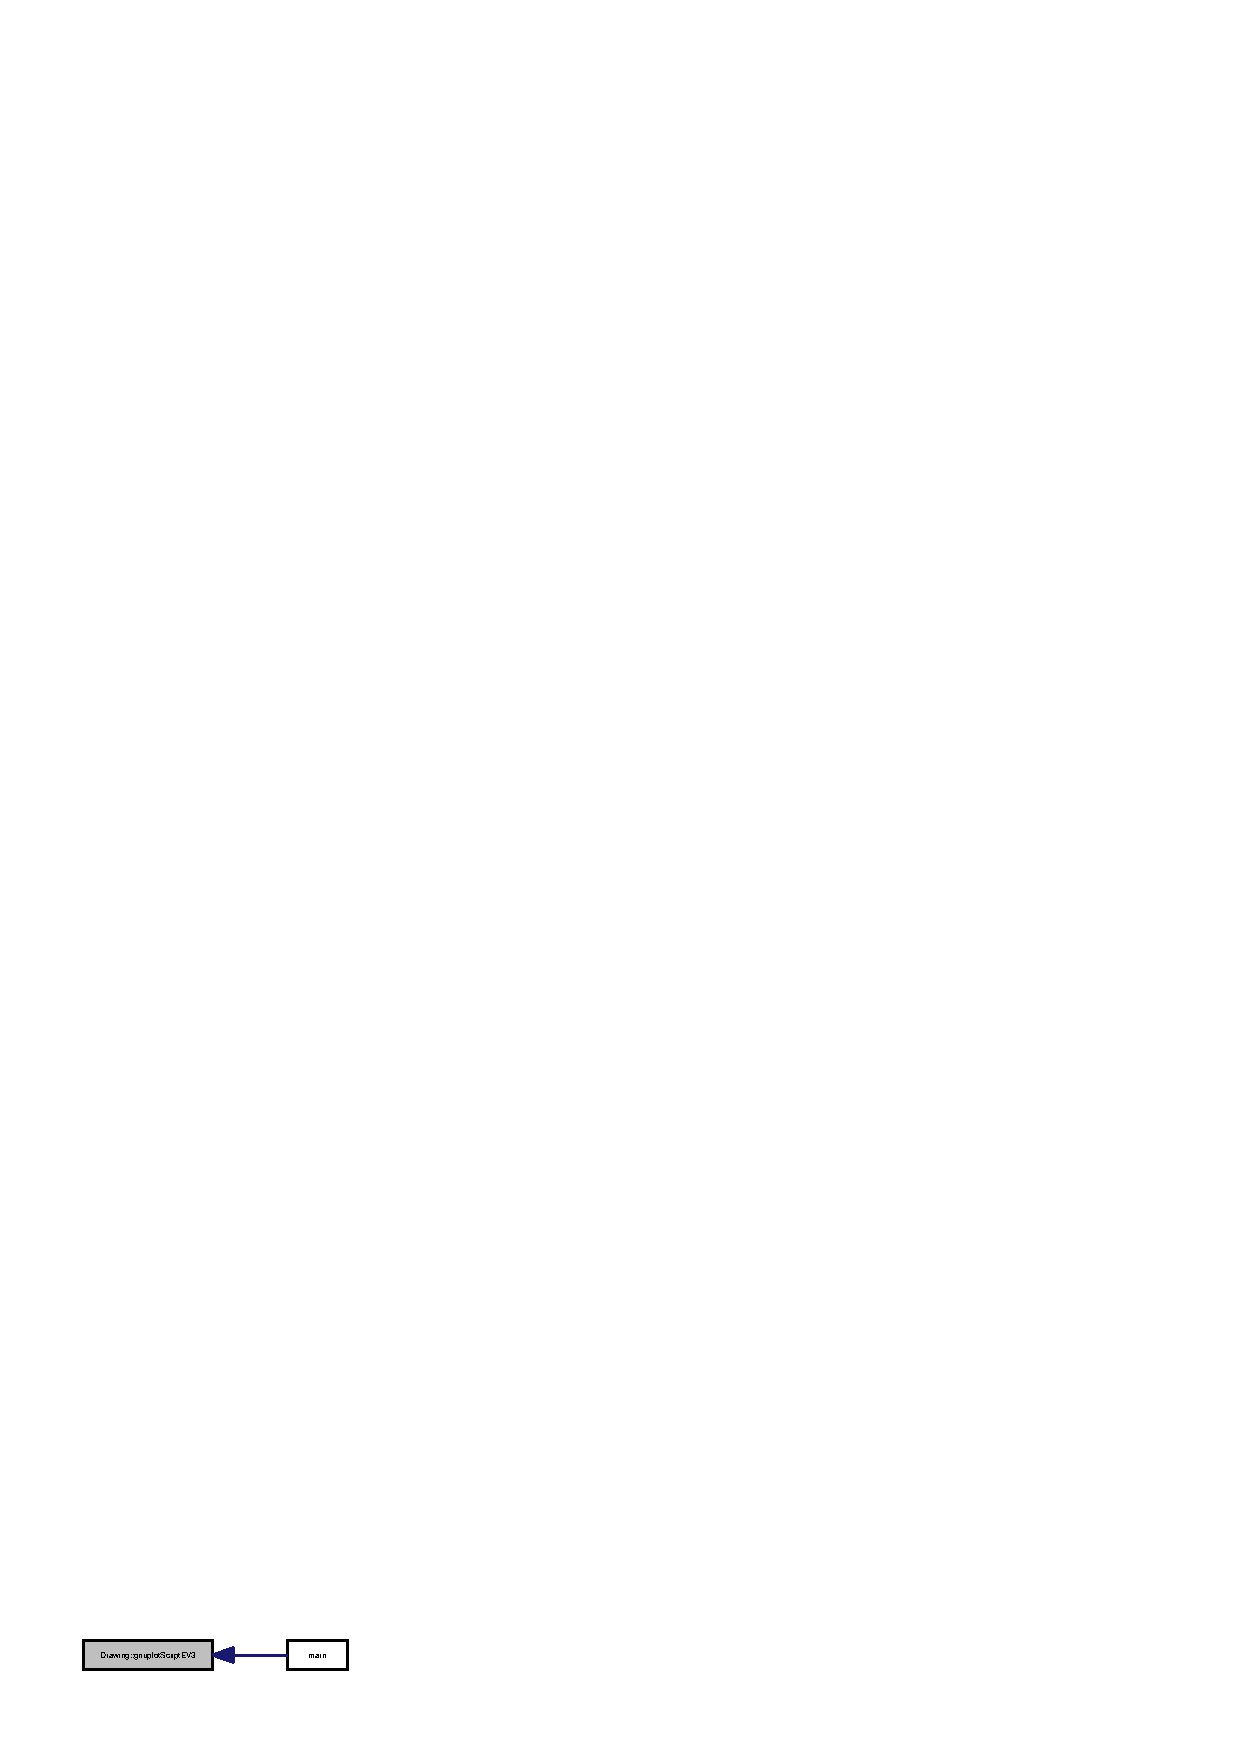
\includegraphics[width=171pt]{class_drawing_a98e39cb40a24d5909954c17fc1eaaa4f_icgraph}
\end{center}
\end{figure}


\index{Drawing@{Drawing}!gnuplot\-Script\-E\-V3\-Route@{gnuplot\-Script\-E\-V3\-Route}}
\index{gnuplot\-Script\-E\-V3\-Route@{gnuplot\-Script\-E\-V3\-Route}!Drawing@{Drawing}}
\subsubsection[{gnuplot\-Script\-E\-V3\-Route}]{\setlength{\rightskip}{0pt plus 5cm}void Drawing\-::gnuplot\-Script\-E\-V3\-Route (
\begin{DoxyParamCaption}
\item[{char $\ast$}]{original\-\_\-dirpath, }
\item[{char $\ast$}]{output\-\_\-filename}
\end{DoxyParamCaption}
)}\label{class_drawing_ac6357919dea1fea41ae447837abcd16b}


E\-V3の軌道をプロットするためのスクリプト 

メソッド\-Drawing\-::gnuplot\-Script\-E\-V3\-Route().\-E\-V3の軌道をプロットするためのスクリプト


\begin{DoxyParams}{引数}
{\em original\-\_\-dirpath} & char$\ast$型.基となるディレクトリ名 \\
\hline
{\em output\-\_\-filename} & char$\ast$型.出力するファイル名 \\
\hline
\end{DoxyParams}


 Drawing.\-cpp の 72 行目に定義があります。



参照先 N\-O\-C.



参照元 main().



被呼び出し関係図\-:\nopagebreak
\begin{figure}[H]
\begin{center}
\leavevmode
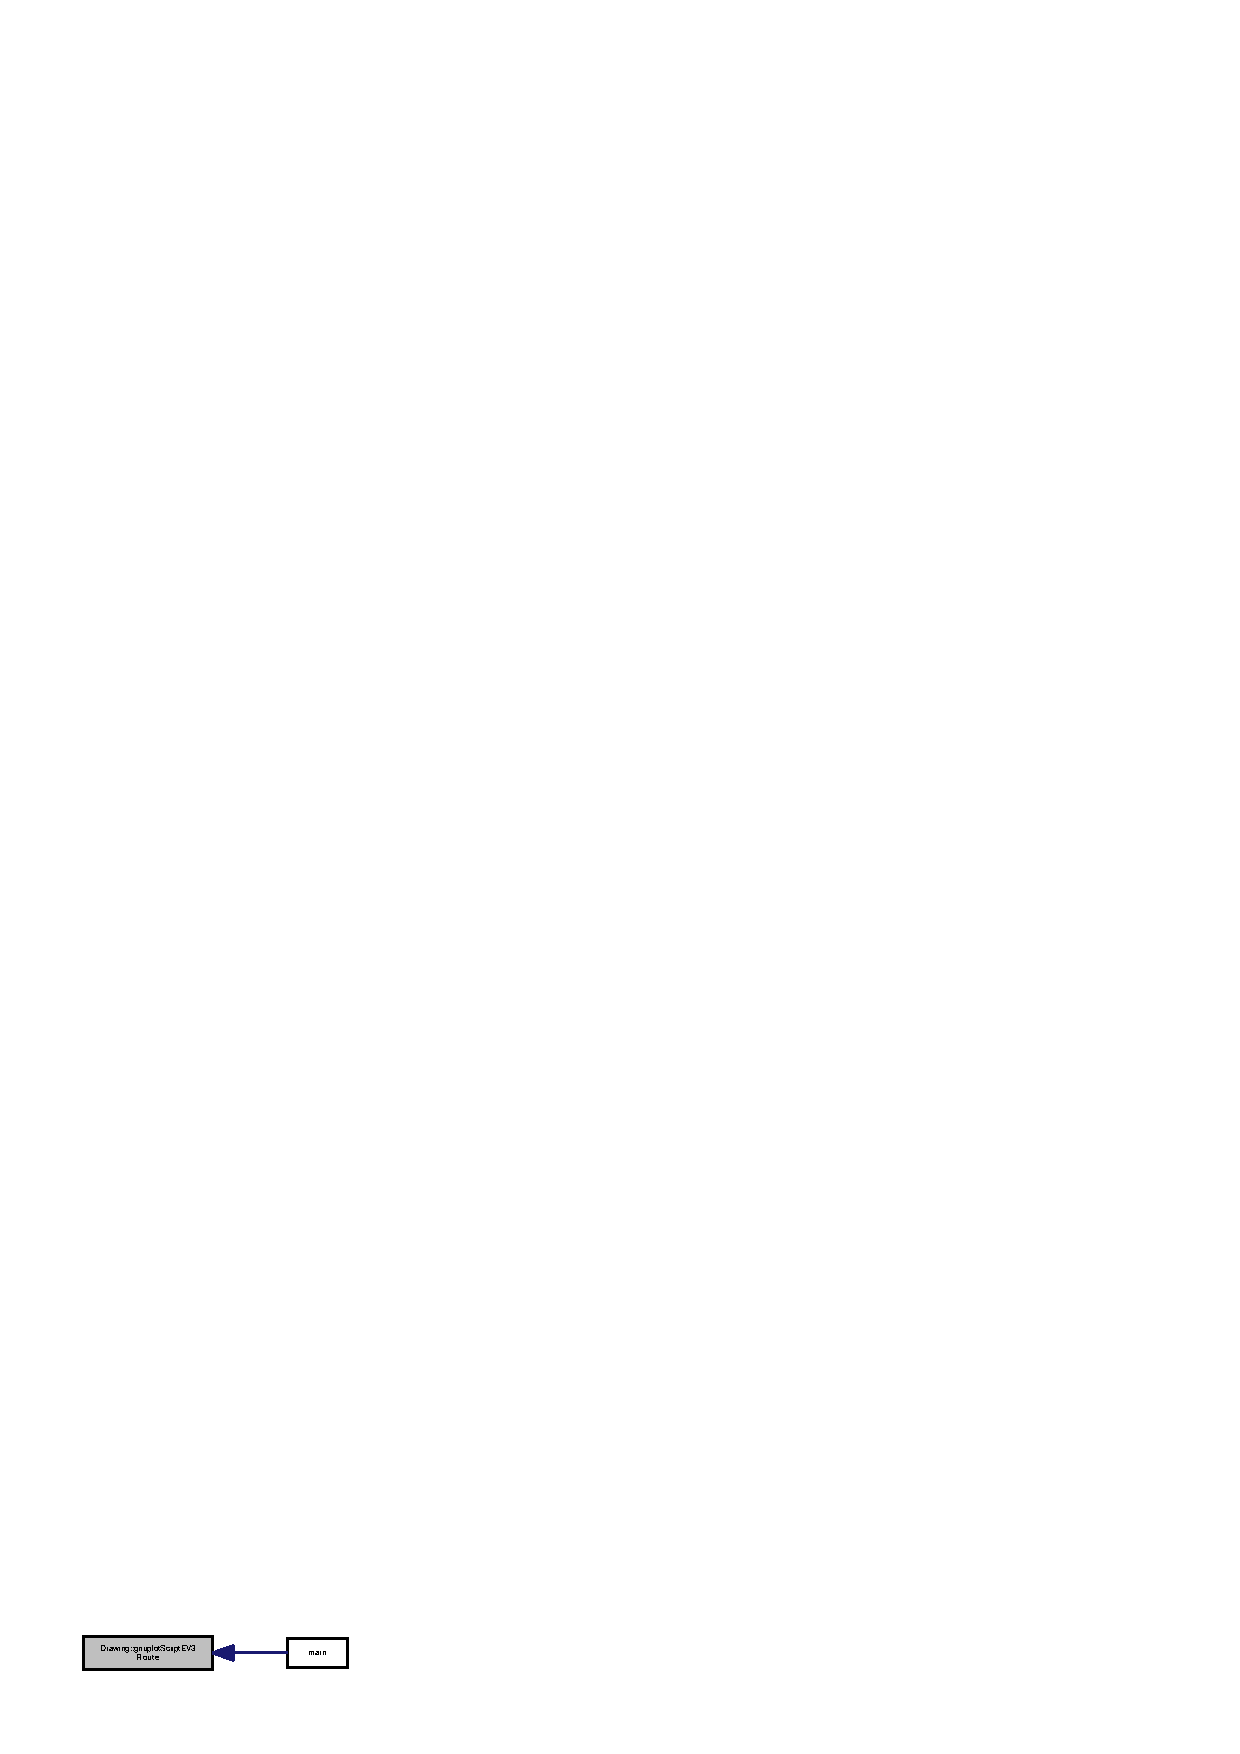
\includegraphics[width=171pt]{class_drawing_ac6357919dea1fea41ae447837abcd16b_icgraph}
\end{center}
\end{figure}


\index{Drawing@{Drawing}!gnuplot\-Script\-Time2\-V@{gnuplot\-Script\-Time2\-V}}
\index{gnuplot\-Script\-Time2\-V@{gnuplot\-Script\-Time2\-V}!Drawing@{Drawing}}
\subsubsection[{gnuplot\-Script\-Time2\-V}]{\setlength{\rightskip}{0pt plus 5cm}void Drawing\-::gnuplot\-Script\-Time2\-V (
\begin{DoxyParamCaption}
{}
\end{DoxyParamCaption}
)}\label{class_drawing_aa1da1f33436ebf7bfc05cf7453a6395e}


時間と速度のプロット 

メソッド\-Drawing\-::gnuplot\-Script\-Time2\-V().時間と速度の関係をプロットするためのスクリプト 

 Drawing.\-cpp の 93 行目に定義があります。



参照先 directory\-Name, N\-O\-C.



参照元 main().



被呼び出し関係図\-:\nopagebreak
\begin{figure}[H]
\begin{center}
\leavevmode
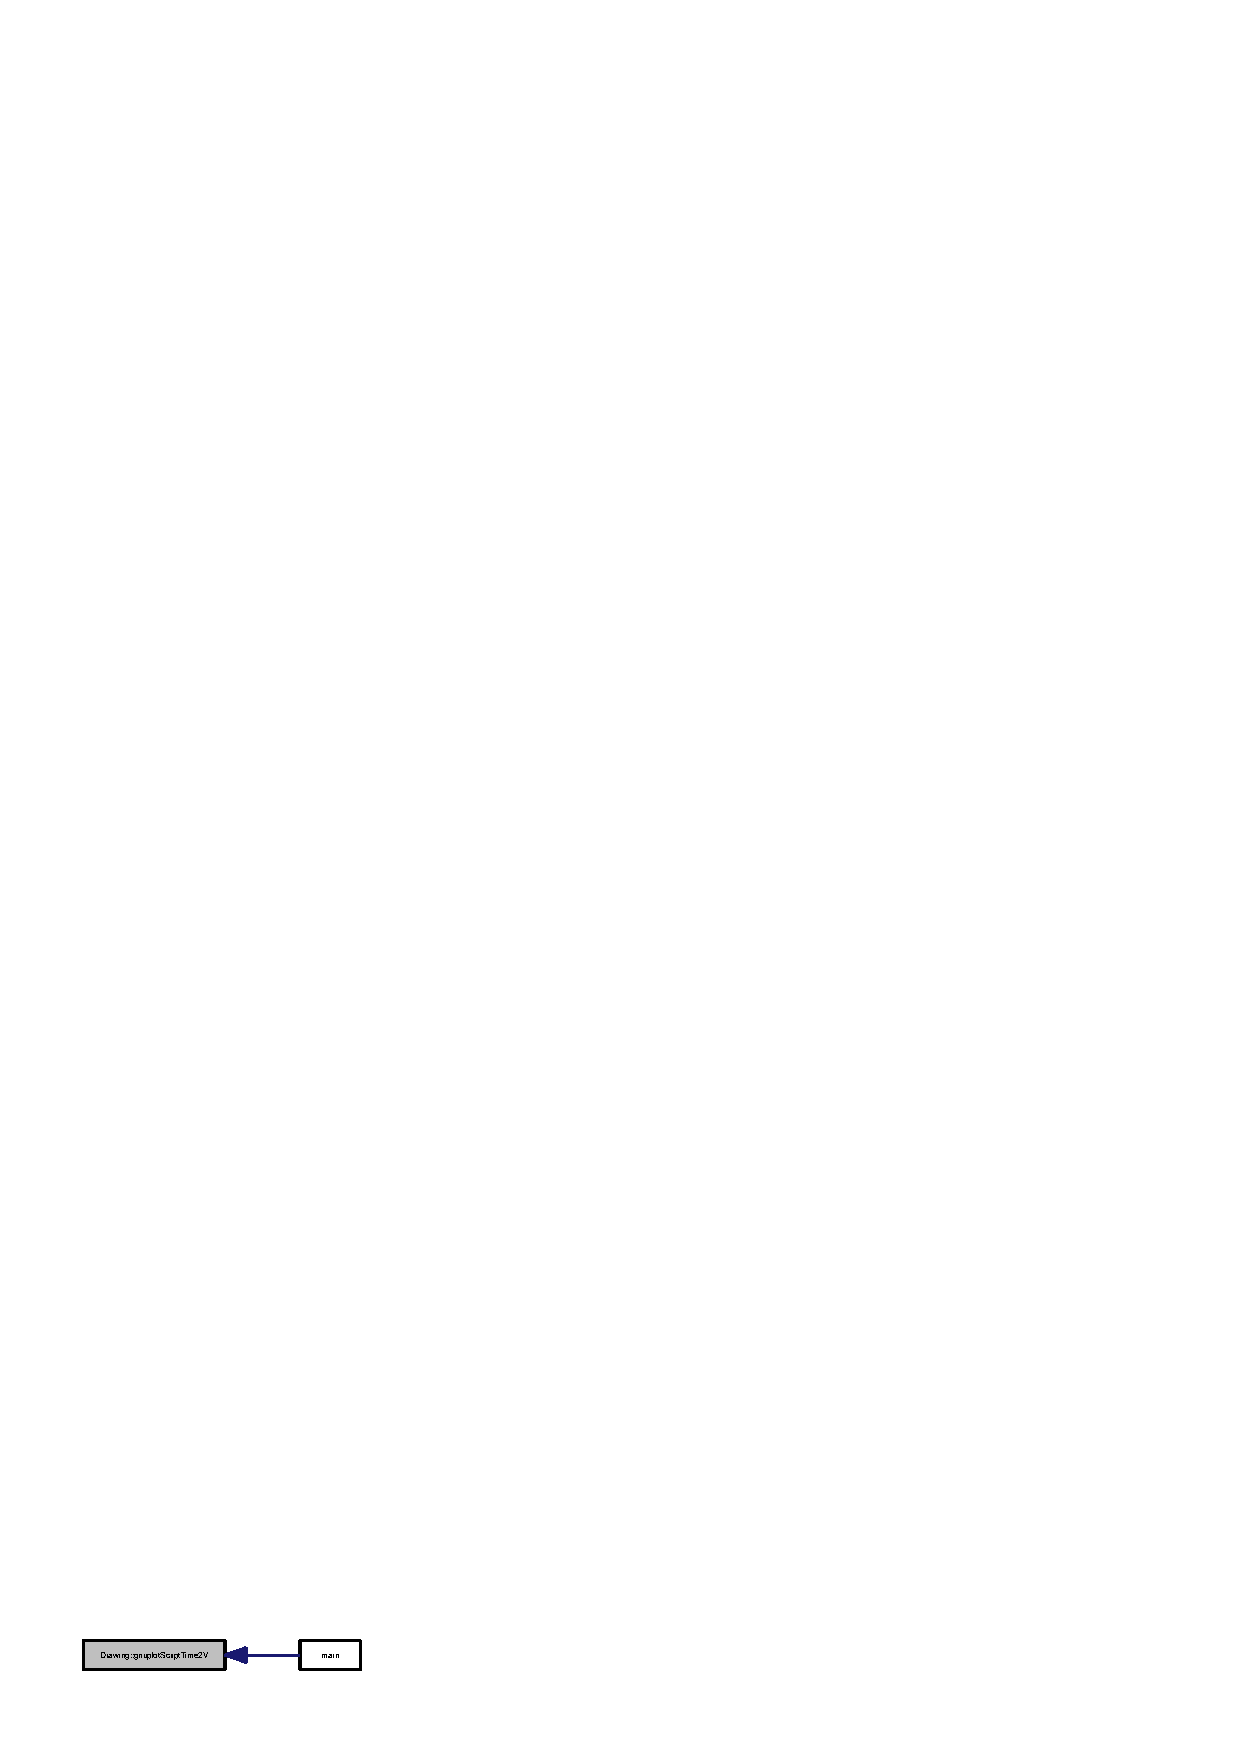
\includegraphics[width=177pt]{class_drawing_aa1da1f33436ebf7bfc05cf7453a6395e_icgraph}
\end{center}
\end{figure}


\index{Drawing@{Drawing}!gnuplot\-Script\-Time2\-Yaw@{gnuplot\-Script\-Time2\-Yaw}}
\index{gnuplot\-Script\-Time2\-Yaw@{gnuplot\-Script\-Time2\-Yaw}!Drawing@{Drawing}}
\subsubsection[{gnuplot\-Script\-Time2\-Yaw}]{\setlength{\rightskip}{0pt plus 5cm}void Drawing\-::gnuplot\-Script\-Time2\-Yaw (
\begin{DoxyParamCaption}
{}
\end{DoxyParamCaption}
)}\label{class_drawing_a4f7e39ba7325c4311761db832d680407}


時間とヨー角のプロット 

メソッド\-Drawing\-::gnuplot\-Script\-Time2\-Yaw().時間とヨー角の関係をプロットするためのスクリプト 

 Drawing.\-cpp の 110 行目に定義があります。



参照先 directory\-Name, N\-O\-C.



参照元 main().



被呼び出し関係図\-:\nopagebreak
\begin{figure}[H]
\begin{center}
\leavevmode
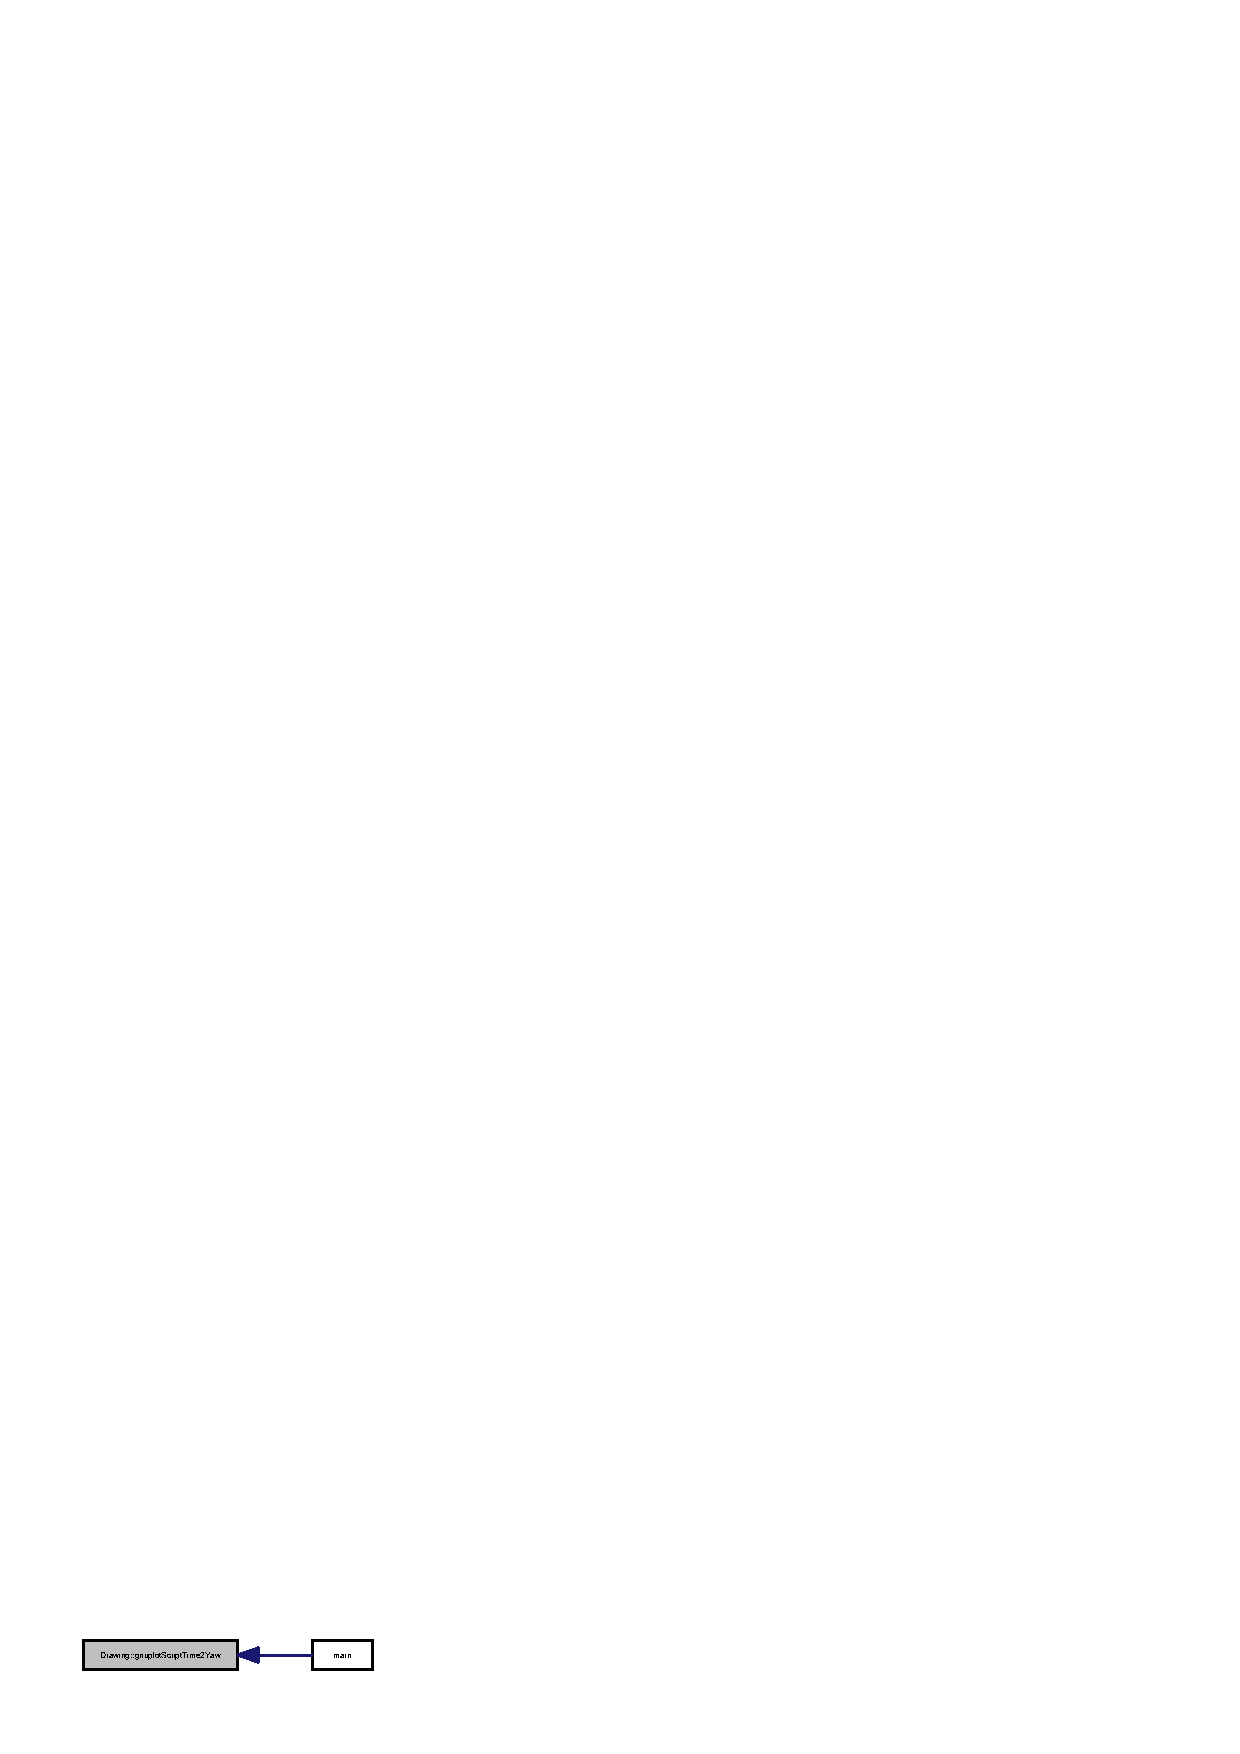
\includegraphics[width=183pt]{class_drawing_a4f7e39ba7325c4311761db832d680407_icgraph}
\end{center}
\end{figure}




このクラス詳解は次のファイルから抽出されました\-:\begin{DoxyCompactItemize}
\item 
{\bf Drawing.\-hpp}\item 
{\bf Drawing.\-cpp}\end{DoxyCompactItemize}

\section{E\-V3\-Control クラス}
\label{class_e_v3_control}\index{E\-V3\-Control@{E\-V3\-Control}}


E\-V3を制御するためのクラス  




{\ttfamily \#include $<$E\-V3\-Control.\-hpp$>$}



E\-V3\-Control 連携図\nopagebreak
\begin{figure}[H]
\begin{center}
\leavevmode
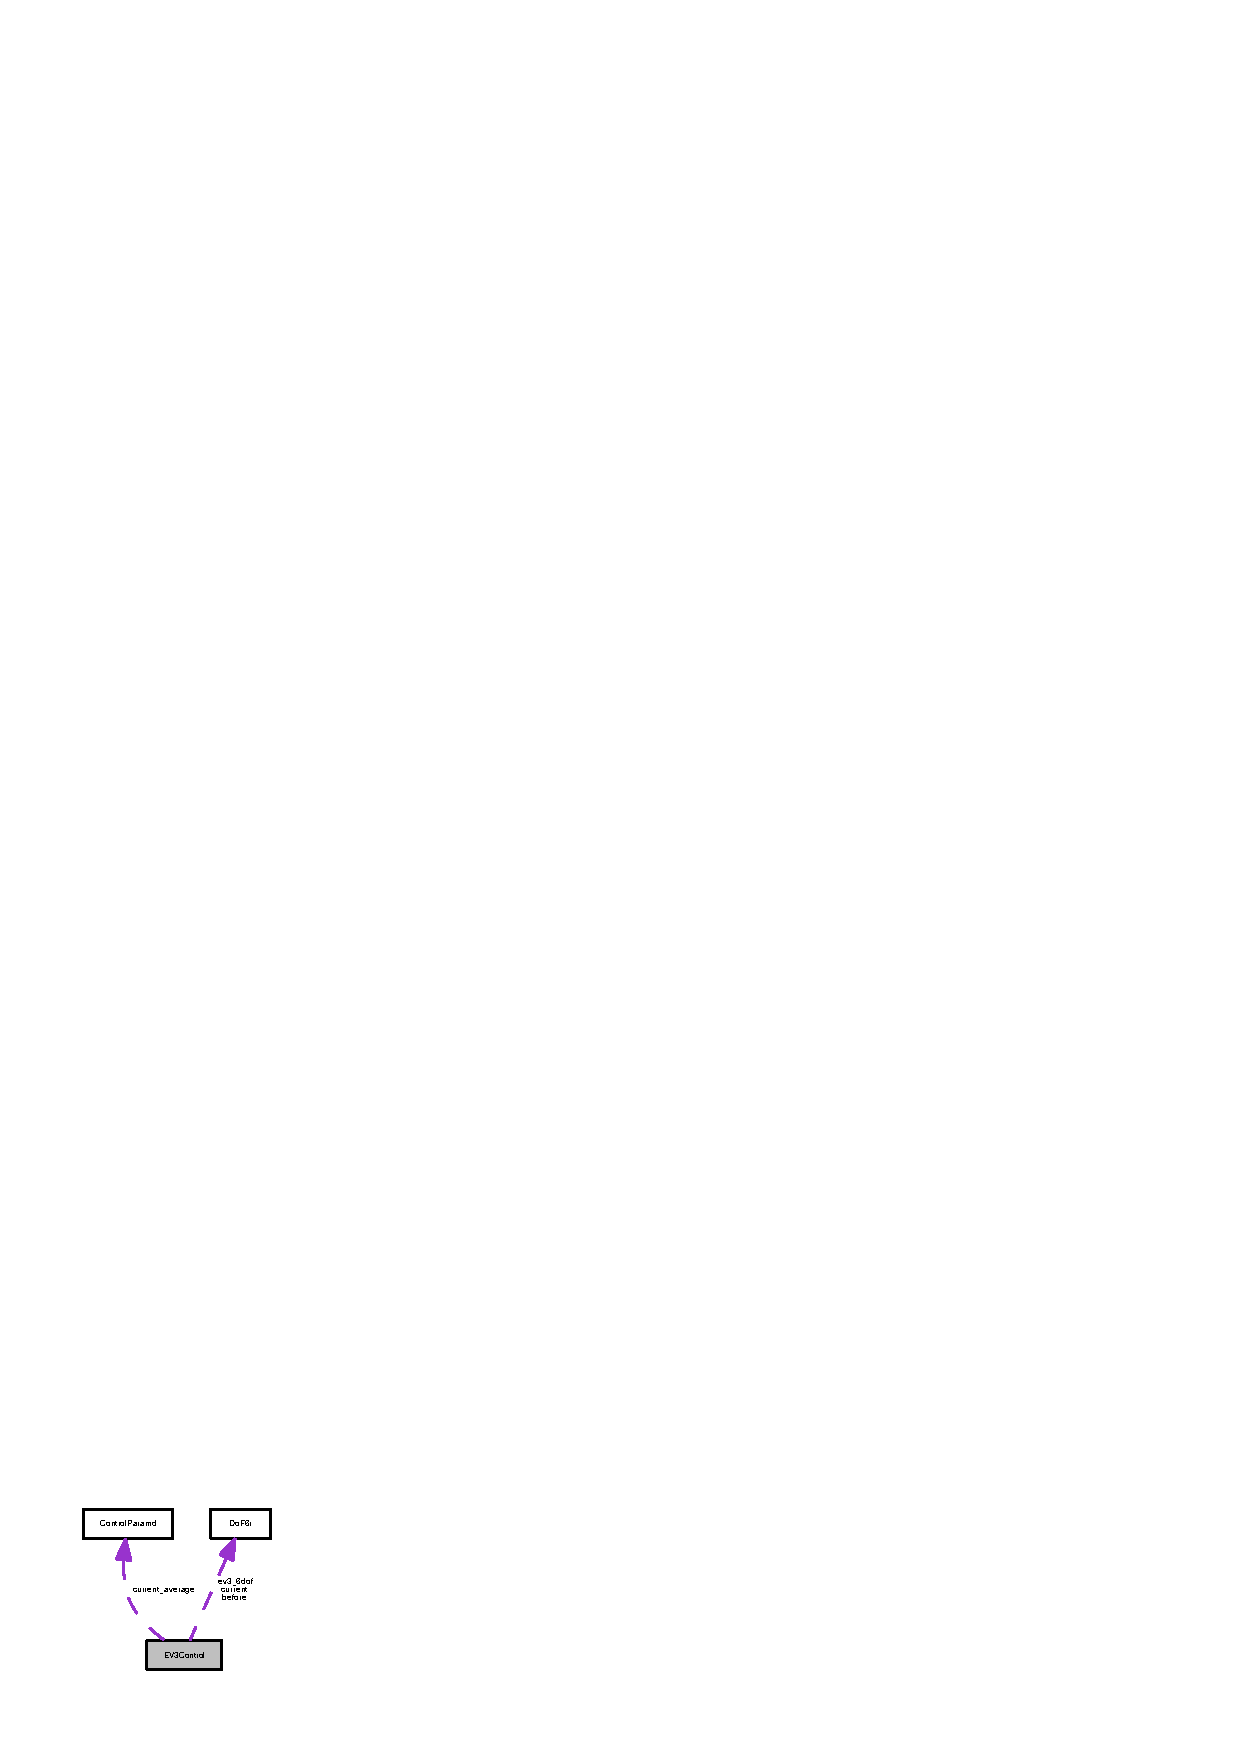
\includegraphics[width=134pt]{class_e_v3_control__coll__graph}
\end{center}
\end{figure}
\subsection*{公開メンバ関数}
\begin{DoxyCompactItemize}
\item 
{\bf E\-V3\-Control} ()
\begin{DoxyCompactList}\small\item\em コンストラクタ \end{DoxyCompactList}\item 
{\bf $\sim$\-E\-V3\-Control} ()
\begin{DoxyCompactList}\small\item\em デストラクタ \end{DoxyCompactList}\item 
void {\bf set6\-Do\-F\-E\-V3} (pcl\-::\-Point\-Cloud$<$ pcl\-::\-Point\-X\-Y\-Z\-R\-G\-B $>$\-::Ptr \&input\-Point\-Cloud, Point3d centroid, {\bf Attitude\-Angle} attitude\-\_\-angle)
\begin{DoxyCompactList}\small\item\em 最小二乗法によって求めた平均座標と位置を\-E\-V3の制御のために構造体に格納する(c80) \end{DoxyCompactList}\item 
void {\bf get\-Velocityin\-Sec} (double time\-\_\-ms)
\begin{DoxyCompactList}\small\item\em E\-V3の速度を計算する(c85) \end{DoxyCompactList}\item 
void {\bf get\-Average\-Velocity\-And\-Yaw} ()
\begin{DoxyCompactList}\small\item\em 平均の速度とヨー角を計算する \end{DoxyCompactList}\item 
void {\bf output6\-Do\-F} (int save\-\_\-count, char $\ast$original\-\_\-dirpath, char $\ast$output\-\_\-filename, pcl\-::\-Point\-Cloud$<$ pcl\-::\-Point\-X\-Y\-Z\-R\-G\-B $>$\-::Ptr \&output\-Point\-Cloud)
\begin{DoxyCompactList}\small\item\em 現フレームの6\-Do\-F情報をファイルに出力する \end{DoxyCompactList}\item 
void {\bf output6\-Do\-F\-Continuous} (char $\ast$original\-\_\-dirpath, char $\ast$output\-\_\-filename, pcl\-::\-Point\-Cloud$<$ pcl\-::\-Point\-X\-Y\-Z\-R\-G\-B $>$\-::Ptr \&output\-Point\-Cloud)
\begin{DoxyCompactList}\small\item\em キーを入力したときの6\-Do\-F情報を連続してcsv形式で保存する \end{DoxyCompactList}\item 
void {\bf output\-E\-V3\-Route\-Continuous} (char $\ast$original\-\_\-dirpath, char $\ast$output\-\_\-filename)
\begin{DoxyCompactList}\small\item\em E\-V3の走行軌道を保存する \end{DoxyCompactList}\item 
void {\bf output\-Control\-Information} (double sumtime\-\_\-ms, char $\ast$original\-\_\-dirpath, char $\ast$output\-\_\-filename)
\begin{DoxyCompactList}\small\item\em E\-V3の制御情報を出力する \end{DoxyCompactList}\item 
void {\bf output\-Control\-Information} ()
\begin{DoxyCompactList}\small\item\em E\-V3に必要な速度とヨー角をファイルに出力 \end{DoxyCompactList}\end{DoxyCompactItemize}
\subsection*{公開変数類}
\begin{DoxyCompactItemize}
\item 
{\bf Do\-F6i} {\bf ev3\-\_\-6dof}
\begin{DoxyCompactList}\small\item\em E\-V3の6自由度(c80) \end{DoxyCompactList}\item 
{\bf Do\-F6i} {\bf before}
\begin{DoxyCompactList}\small\item\em 前フレームの6\-Do\-F情報 \end{DoxyCompactList}\item 
{\bf Do\-F6i} {\bf current}
\begin{DoxyCompactList}\small\item\em 現フレームの6\-Do\-F情報 \end{DoxyCompactList}\item 
double {\bf velocity}
\begin{DoxyCompactList}\small\item\em 速度v(c85) \end{DoxyCompactList}\item 
bool {\bf flag\-\_\-velocity}
\begin{DoxyCompactList}\small\item\em 最初の1フレームのためのフラグ \end{DoxyCompactList}\item 
{\bf Control\-Paramd} {\bf current\-\_\-average}
\begin{DoxyCompactList}\small\item\em 現在の平均の速度とヨー角 \end{DoxyCompactList}\item 
int {\bf count\-\_\-average}
\begin{DoxyCompactList}\small\item\em 速度とヨー角の過去5フレーム分の平均を取るために最初の5フレームをカウントするための変数 \end{DoxyCompactList}\item 
bool {\bf flag\-\_\-average}
\begin{DoxyCompactList}\small\item\em 始めの5フレーム分用 \end{DoxyCompactList}\item 
bool {\bf save\-\_\-flag}
\begin{DoxyCompactList}\small\item\em 6\-Do\-F情報を出力するかチェックするためのフラグ \end{DoxyCompactList}\end{DoxyCompactItemize}


\subsection{詳解}
E\-V3を制御するためのクラス 

 E\-V3\-Control.\-hpp の 18 行目に定義があります。



\subsection{構築子と解体子}
\index{E\-V3\-Control@{E\-V3\-Control}!E\-V3\-Control@{E\-V3\-Control}}
\index{E\-V3\-Control@{E\-V3\-Control}!EV3Control@{E\-V3\-Control}}
\subsubsection[{E\-V3\-Control}]{\setlength{\rightskip}{0pt plus 5cm}E\-V3\-Control\-::\-E\-V3\-Control (
\begin{DoxyParamCaption}
{}
\end{DoxyParamCaption}
)}\label{class_e_v3_control_a030f467b372dee725bb176d0b7cea259}


コンストラクタ 

メソッド\-E\-V3\-Control\-::\-E\-V3\-Control().コンストラクタ 

 E\-V3\-Control.\-cpp の 15 行目に定義があります。



参照先 before, count\-\_\-average, current, current\-\_\-average, flag\-\_\-average, flag\-\_\-velocity, save\-\_\-flag.

\index{E\-V3\-Control@{E\-V3\-Control}!$\sim$\-E\-V3\-Control@{$\sim$\-E\-V3\-Control}}
\index{$\sim$\-E\-V3\-Control@{$\sim$\-E\-V3\-Control}!EV3Control@{E\-V3\-Control}}
\subsubsection[{$\sim$\-E\-V3\-Control}]{\setlength{\rightskip}{0pt plus 5cm}E\-V3\-Control\-::$\sim$\-E\-V3\-Control (
\begin{DoxyParamCaption}
{}
\end{DoxyParamCaption}
)}\label{class_e_v3_control_a68c7fd119aa2f422f9eebbe9318e8ab9}


デストラクタ 

メソッド\-E\-V3\-Control\-::\-E\-V3\-Control().コンストラクタ 

 E\-V3\-Control.\-cpp の 38 行目に定義があります。



\subsection{関数詳解}
\index{E\-V3\-Control@{E\-V3\-Control}!get\-Average\-Velocity\-And\-Yaw@{get\-Average\-Velocity\-And\-Yaw}}
\index{get\-Average\-Velocity\-And\-Yaw@{get\-Average\-Velocity\-And\-Yaw}!EV3Control@{E\-V3\-Control}}
\subsubsection[{get\-Average\-Velocity\-And\-Yaw}]{\setlength{\rightskip}{0pt plus 5cm}void E\-V3\-Control\-::get\-Average\-Velocity\-And\-Yaw (
\begin{DoxyParamCaption}
{}
\end{DoxyParamCaption}
)}\label{class_e_v3_control_a2231f75bbba634cbb018ec9bf2de75a0}


平均の速度とヨー角を計算する 

メソッド\-E\-V3\-Control\-::get\-Average\-Velocity\-And\-Yaw().速度とヨー角を取得するメソッド 

 E\-V3\-Control.\-cpp の 89 行目に定義があります。



参照先 count\-\_\-average, current\-\_\-average, ev3\-\_\-6dof, flag\-\_\-average, velocity, Control\-Paramd\-::velocity, Do\-F6i\-::yaw, Control\-Paramd\-::yaw.



参照元 main().



被呼び出し関係図\-:\nopagebreak
\begin{figure}[H]
\begin{center}
\leavevmode
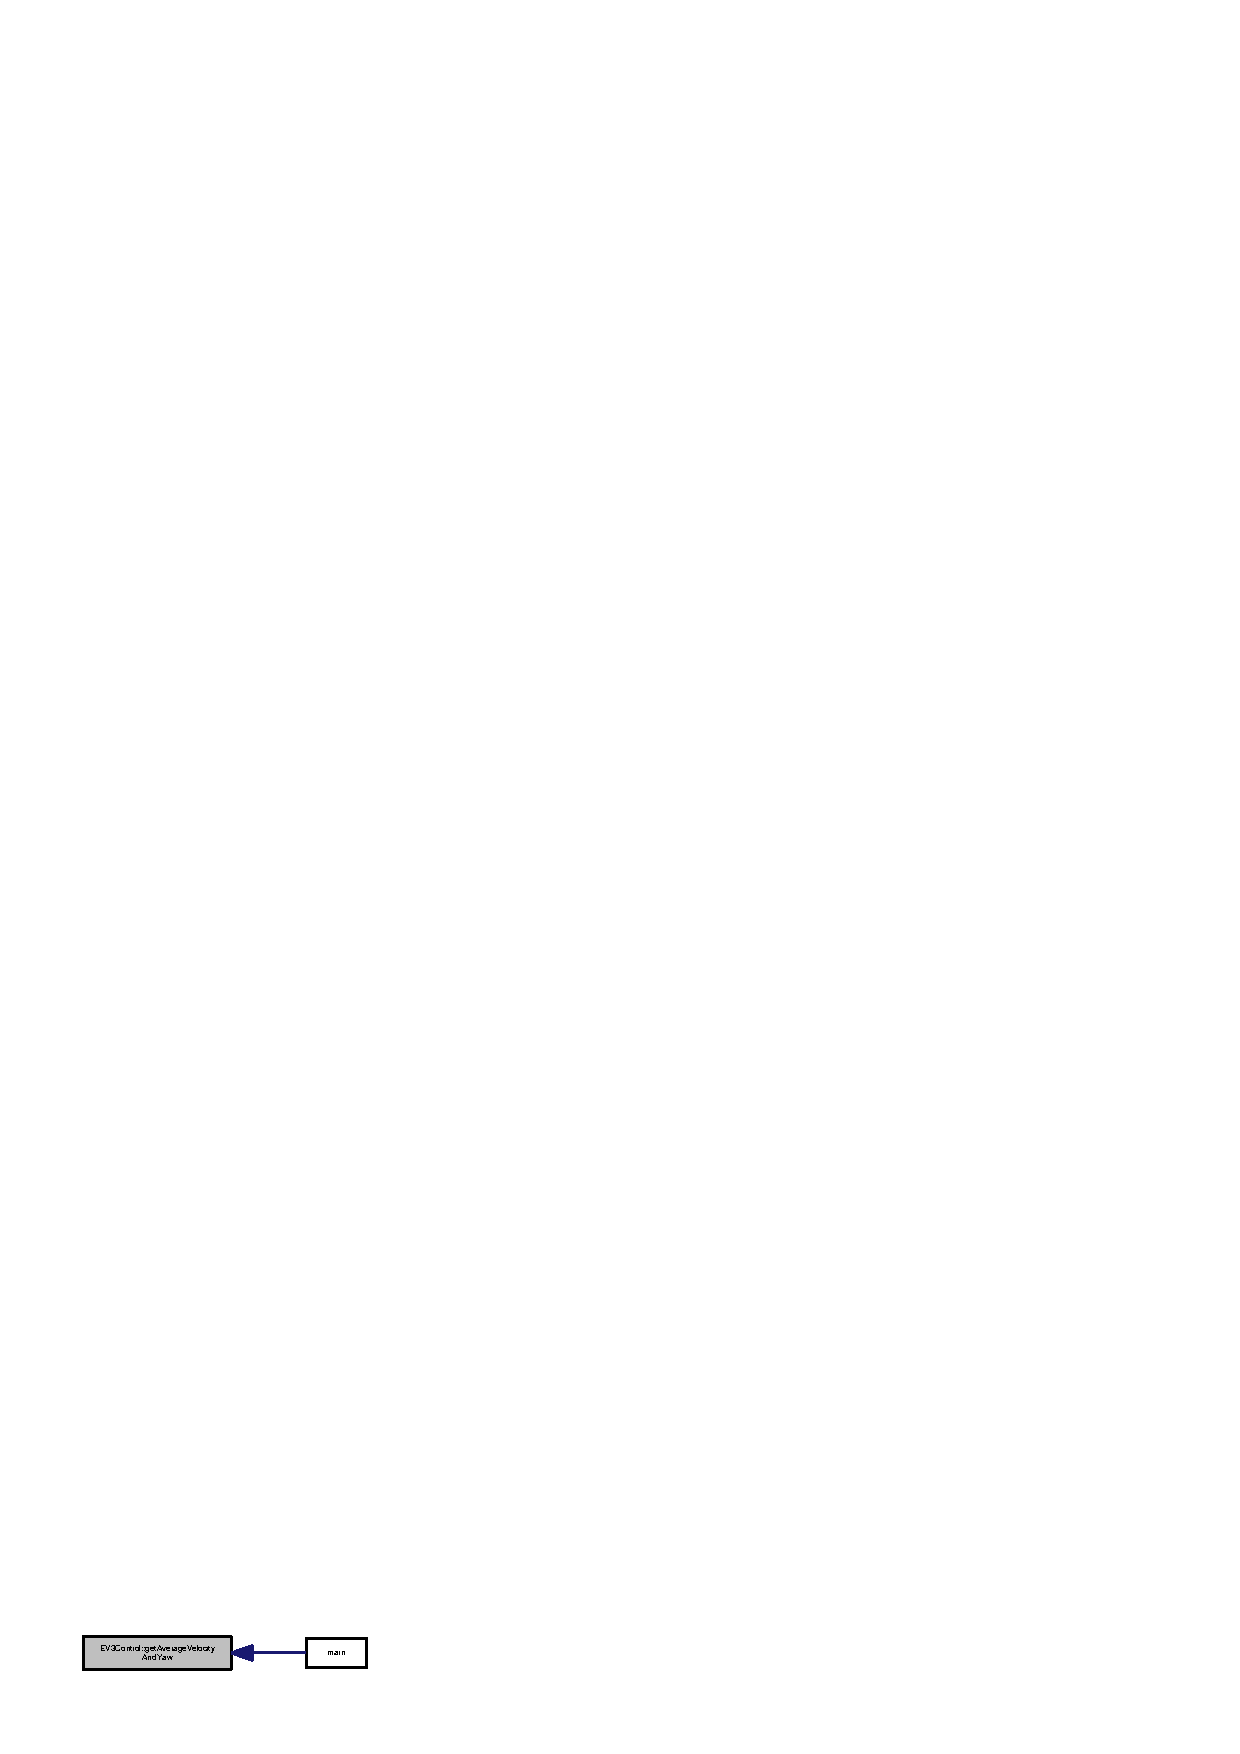
\includegraphics[width=180pt]{class_e_v3_control_a2231f75bbba634cbb018ec9bf2de75a0_icgraph}
\end{center}
\end{figure}


\index{E\-V3\-Control@{E\-V3\-Control}!get\-Velocityin\-Sec@{get\-Velocityin\-Sec}}
\index{get\-Velocityin\-Sec@{get\-Velocityin\-Sec}!EV3Control@{E\-V3\-Control}}
\subsubsection[{get\-Velocityin\-Sec}]{\setlength{\rightskip}{0pt plus 5cm}void E\-V3\-Control\-::get\-Velocityin\-Sec (
\begin{DoxyParamCaption}
\item[{double}]{time\-\_\-ms}
\end{DoxyParamCaption}
)}\label{class_e_v3_control_a206f5da82bb48c5ddae1906b9206d773}


E\-V3の速度を計算する(c85) 

メソッド\-E\-V3\-Control\-::get\-Velocity().\-E\-V3の速度を計算するメソッド


\begin{DoxyParams}{引数}
{\em time\-\_\-ms} & double型.1フレームの処理時間 \\
\hline
\end{DoxyParams}


 E\-V3\-Control.\-cpp の 67 行目に定義があります。



参照先 before, current, ev3\-\_\-6dof, flag\-\_\-velocity, velocity, Do\-F6i\-::x, Do\-F6i\-::y, Do\-F6i\-::z.



参照元 main().



被呼び出し関係図\-:\nopagebreak
\begin{figure}[H]
\begin{center}
\leavevmode
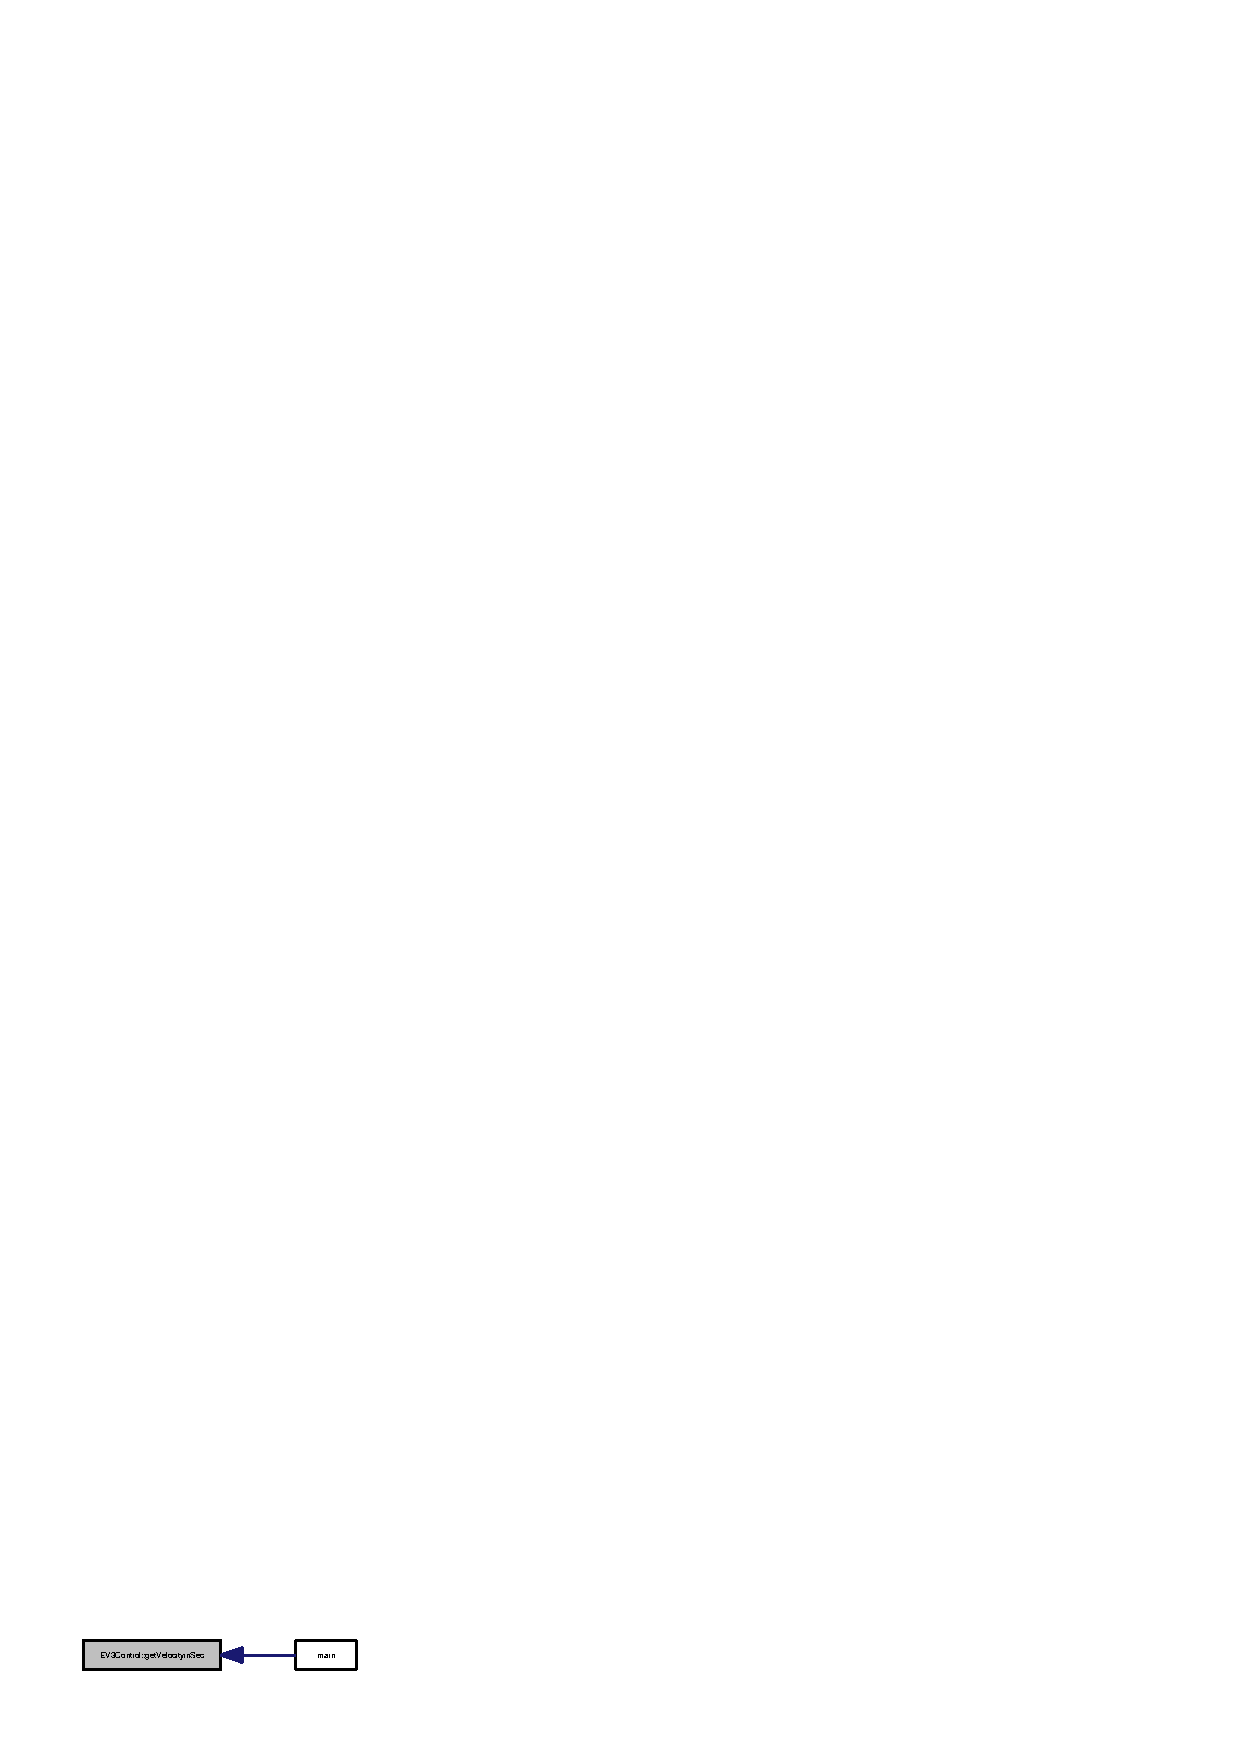
\includegraphics[width=175pt]{class_e_v3_control_a206f5da82bb48c5ddae1906b9206d773_icgraph}
\end{center}
\end{figure}


\index{E\-V3\-Control@{E\-V3\-Control}!output6\-Do\-F@{output6\-Do\-F}}
\index{output6\-Do\-F@{output6\-Do\-F}!EV3Control@{E\-V3\-Control}}
\subsubsection[{output6\-Do\-F}]{\setlength{\rightskip}{0pt plus 5cm}void E\-V3\-Control\-::output6\-Do\-F (
\begin{DoxyParamCaption}
\item[{int}]{save\-\_\-count, }
\item[{char $\ast$}]{original\-\_\-dirpath, }
\item[{char $\ast$}]{output\-\_\-filename, }
\item[{pcl\-::\-Point\-Cloud$<$ pcl\-::\-Point\-X\-Y\-Z\-R\-G\-B $>$\-::Ptr \&}]{output\-Point\-Cloud}
\end{DoxyParamCaption}
)}\label{class_e_v3_control_afce936155dcdef2787d31741b2bb1868}


現フレームの6\-Do\-F情報をファイルに出力する 

メソッド\-E\-V3\-Control\-::output6\-Dof().現フレームの6\-Do\-F情報をファイルに出力する


\begin{DoxyParams}{引数}
{\em save\-\_\-count} & int型.保存したカウント \\
\hline
{\em original\-\_\-dirpath} & char$\ast$型.基となるディレクトリ名 \\
\hline
{\em output\-\_\-filename} & char$\ast$型.出力するファイル名 \\
\hline
\end{DoxyParams}


 E\-V3\-Control.\-cpp の 150 行目に定義があります。



参照先 ev3\-\_\-6dof, N\-O\-C, Do\-F6i\-::pitch, Do\-F6i\-::roll, Do\-F6i\-::x, Do\-F6i\-::y, Do\-F6i\-::yaw, Do\-F6i\-::z.



参照元 main().



被呼び出し関係図\-:\nopagebreak
\begin{figure}[H]
\begin{center}
\leavevmode
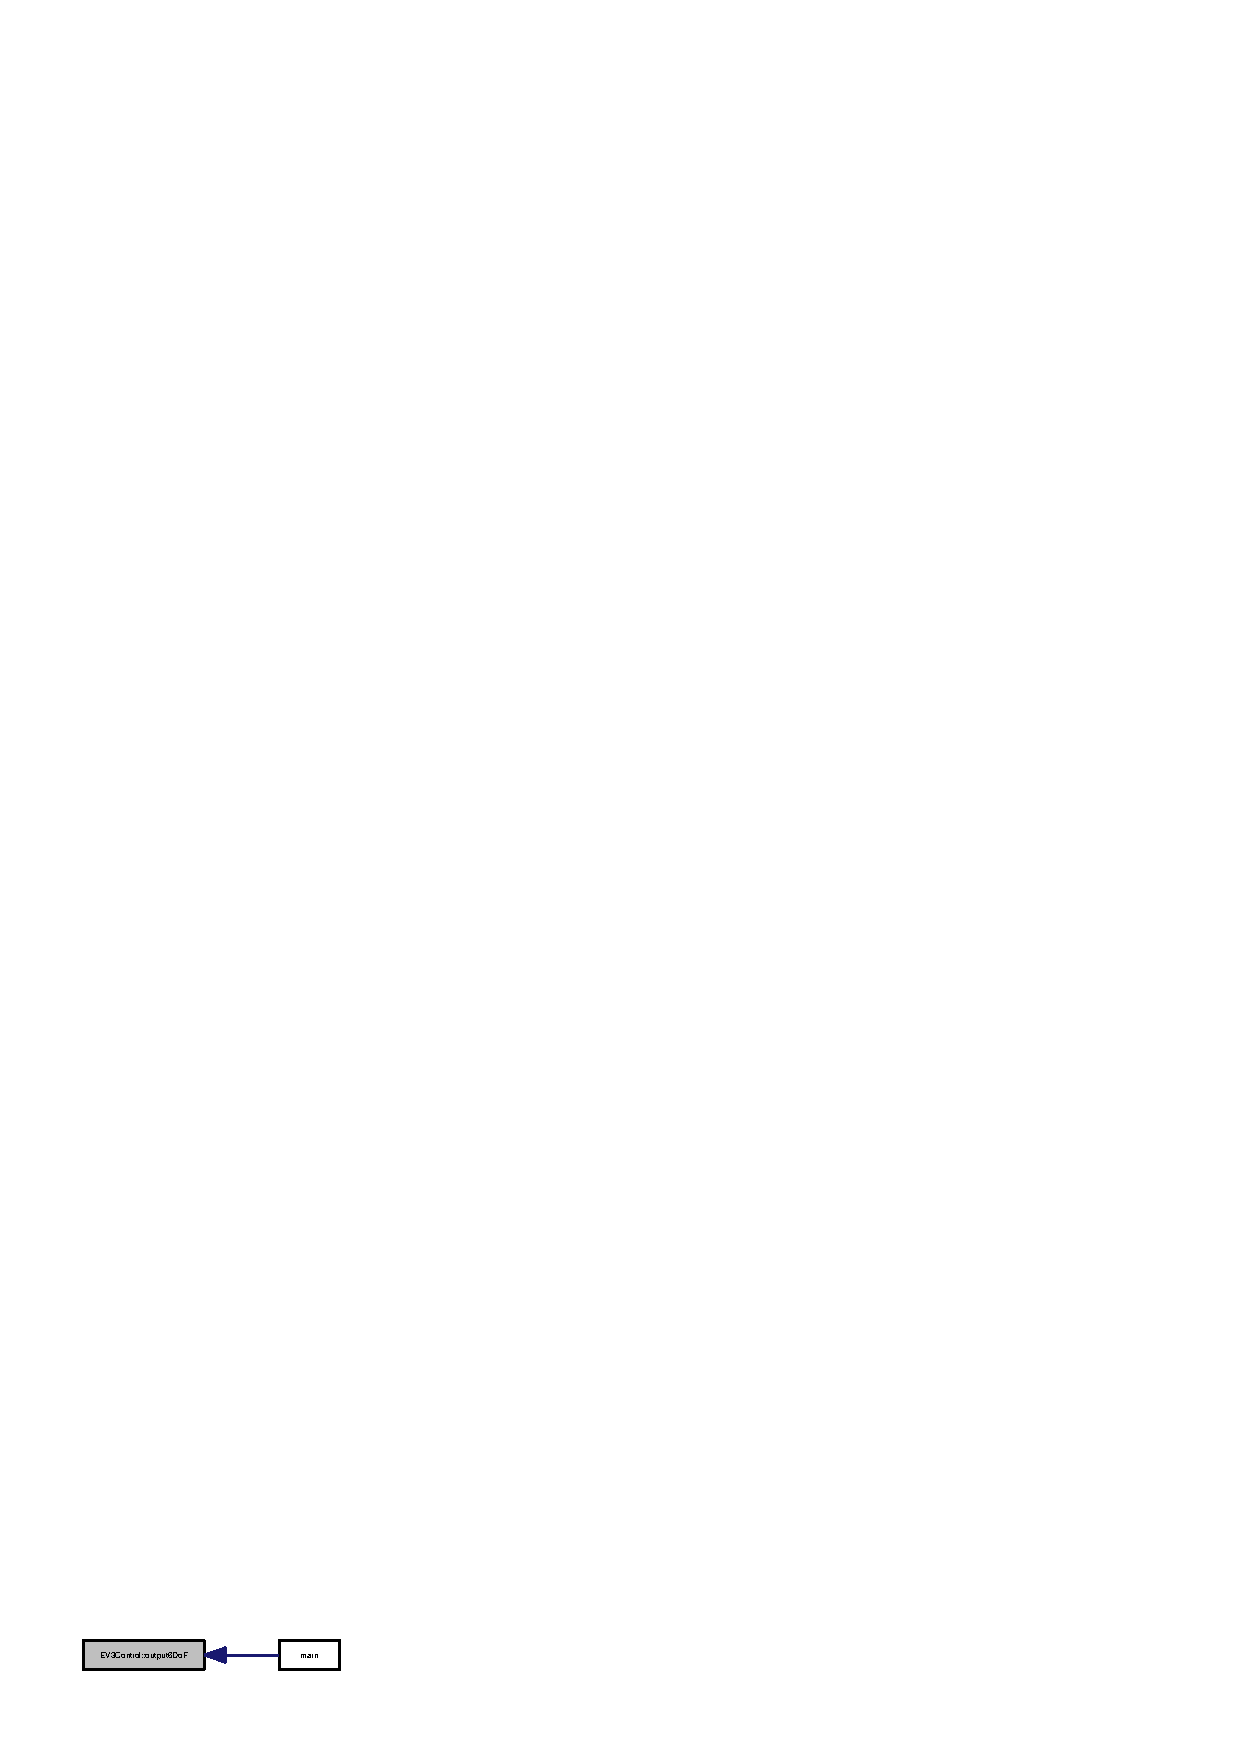
\includegraphics[width=167pt]{class_e_v3_control_afce936155dcdef2787d31741b2bb1868_icgraph}
\end{center}
\end{figure}


\index{E\-V3\-Control@{E\-V3\-Control}!output6\-Do\-F\-Continuous@{output6\-Do\-F\-Continuous}}
\index{output6\-Do\-F\-Continuous@{output6\-Do\-F\-Continuous}!EV3Control@{E\-V3\-Control}}
\subsubsection[{output6\-Do\-F\-Continuous}]{\setlength{\rightskip}{0pt plus 5cm}void E\-V3\-Control\-::output6\-Do\-F\-Continuous (
\begin{DoxyParamCaption}
\item[{char $\ast$}]{original\-\_\-dirpath, }
\item[{char $\ast$}]{output\-\_\-filename, }
\item[{pcl\-::\-Point\-Cloud$<$ pcl\-::\-Point\-X\-Y\-Z\-R\-G\-B $>$\-::Ptr \&}]{output\-Point\-Cloud}
\end{DoxyParamCaption}
)}\label{class_e_v3_control_a8308b078e6fce216a0b5e8e6a502e7ab}


キーを入力したときの6\-Do\-F情報を連続してcsv形式で保存する 

メソッド\-E\-V3\-Control\-::output6\-Do\-F\-Continuous().キーを入力したときの6\-Do\-F情報を連続してcsv形式で保存する


\begin{DoxyParams}{引数}
{\em original\-\_\-dirpath} & char$\ast$型.基となるディレクトリ名 \\
\hline
{\em output\-\_\-filename} & char$\ast$型.出力するファイル名 \\
\hline
{\em \&input\-Point\-Cloud} & pcl\-::\-Point\-Cloud$<$pcl\-::\-Point\-X\-Y\-Z\-R\-G\-B$>$\-::\-Ptr \\
\hline
\end{DoxyParams}


 E\-V3\-Control.\-cpp の 169 行目に定義があります。



参照先 ev3\-\_\-6dof, N\-O\-C, Do\-F6i\-::pitch, Do\-F6i\-::roll, save\-\_\-flag, Do\-F6i\-::x, Do\-F6i\-::y, Do\-F6i\-::yaw, Do\-F6i\-::z.



参照元 main().



被呼び出し関係図\-:\nopagebreak
\begin{figure}[H]
\begin{center}
\leavevmode
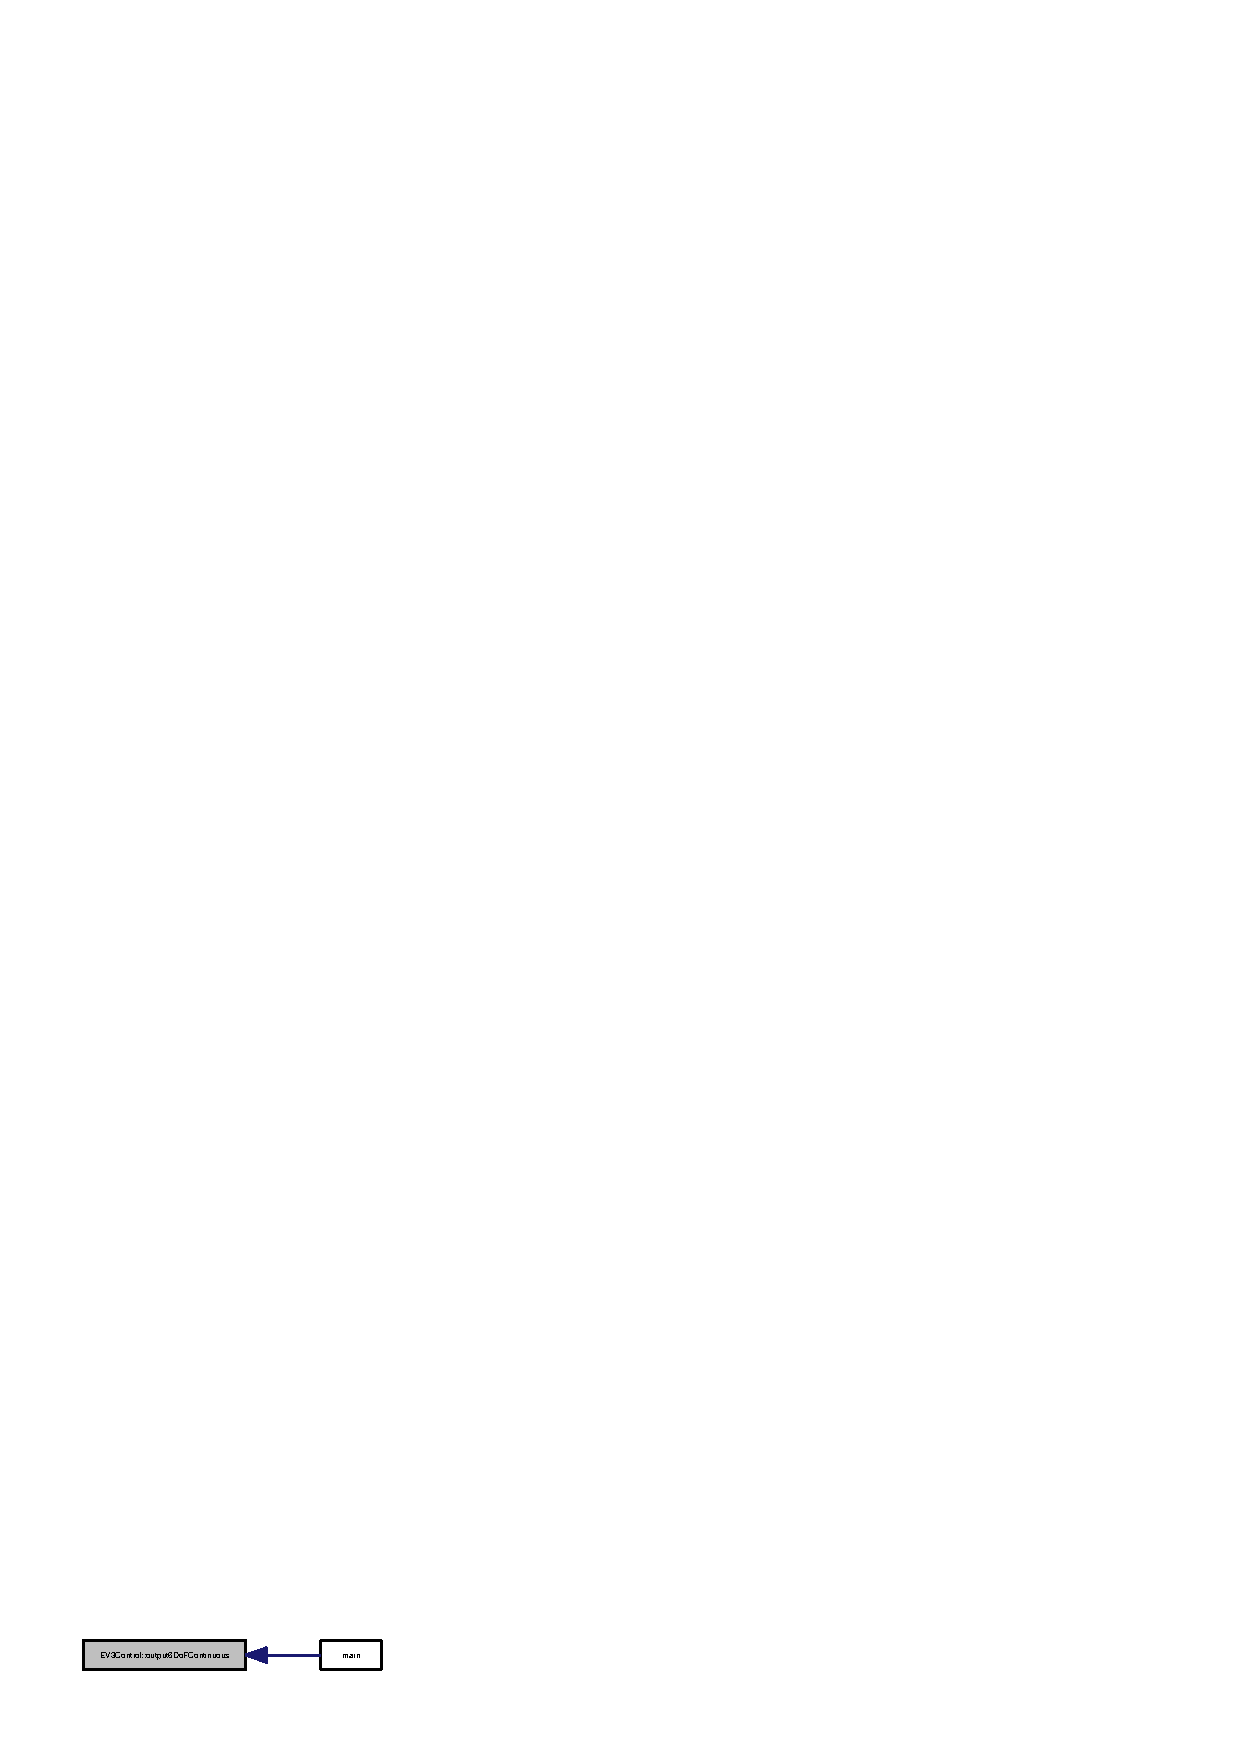
\includegraphics[width=187pt]{class_e_v3_control_a8308b078e6fce216a0b5e8e6a502e7ab_icgraph}
\end{center}
\end{figure}


\index{E\-V3\-Control@{E\-V3\-Control}!output\-Control\-Information@{output\-Control\-Information}}
\index{output\-Control\-Information@{output\-Control\-Information}!EV3Control@{E\-V3\-Control}}
\subsubsection[{output\-Control\-Information}]{\setlength{\rightskip}{0pt plus 5cm}void E\-V3\-Control\-::output\-Control\-Information (
\begin{DoxyParamCaption}
\item[{double}]{sumtime\-\_\-ms, }
\item[{char $\ast$}]{original\-\_\-dirpath, }
\item[{char $\ast$}]{output\-\_\-filename}
\end{DoxyParamCaption}
)}\label{class_e_v3_control_a6bec8596128f406b0a90a6b206e1fd67}


E\-V3の制御情報を出力する 

メソッド\-E\-V3\-Control\-::output\-Control\-Information().\-E\-V3の制御情報を出力する


\begin{DoxyParams}{引数}
{\em sumtime\-\_\-ms} & double型.合計時間 \\
\hline
{\em original\-\_\-dirpath} & char$\ast$型.基となるディレクトリ名 \\
\hline
{\em output\-\_\-filename} & char$\ast$型.出力するファイル名 \\
\hline
\end{DoxyParams}


 E\-V3\-Control.\-cpp の 208 行目に定義があります。



参照先 current\-\_\-average, N\-O\-C, Control\-Paramd\-::velocity, Control\-Paramd\-::yaw.



参照元 main().



被呼び出し関係図\-:\nopagebreak
\begin{figure}[H]
\begin{center}
\leavevmode
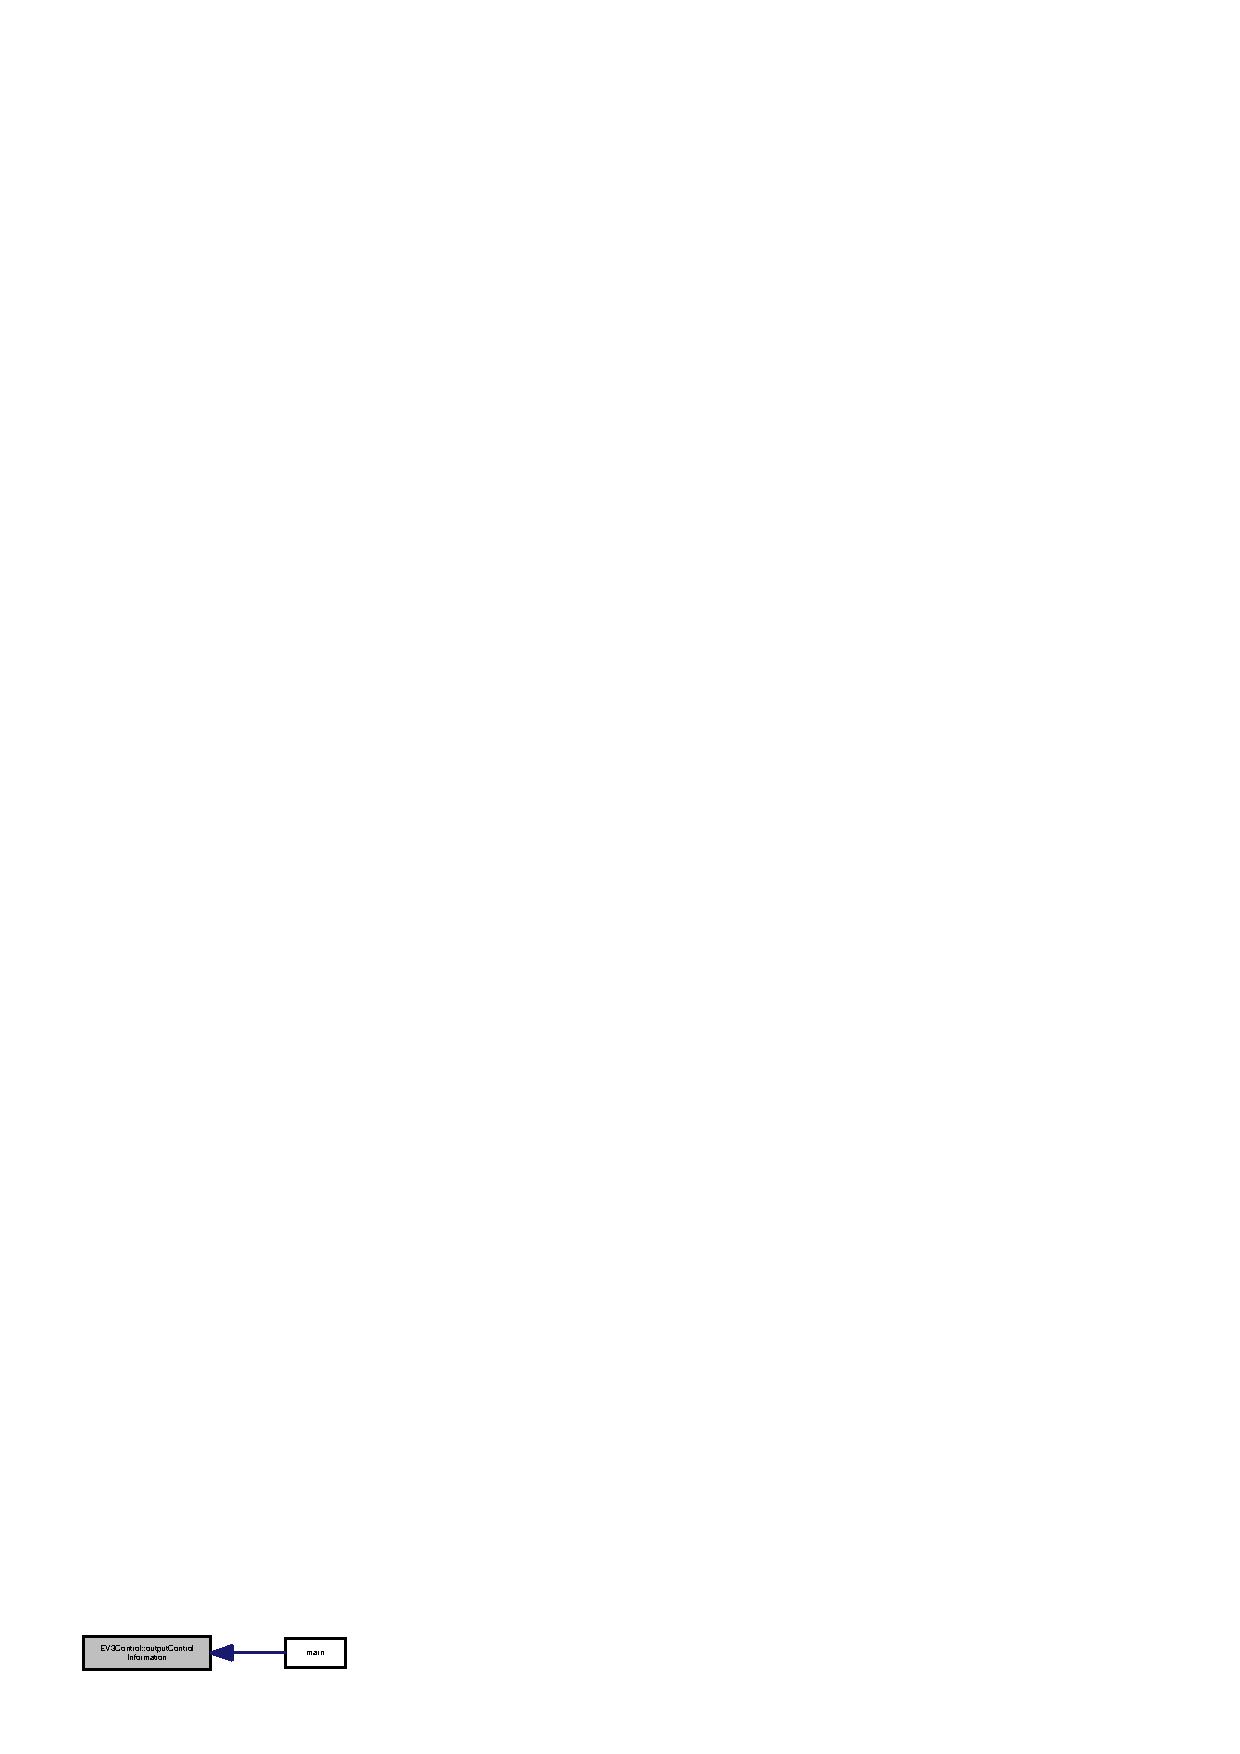
\includegraphics[width=170pt]{class_e_v3_control_a6bec8596128f406b0a90a6b206e1fd67_icgraph}
\end{center}
\end{figure}


\index{E\-V3\-Control@{E\-V3\-Control}!output\-Control\-Information@{output\-Control\-Information}}
\index{output\-Control\-Information@{output\-Control\-Information}!EV3Control@{E\-V3\-Control}}
\subsubsection[{output\-Control\-Information}]{\setlength{\rightskip}{0pt plus 5cm}void E\-V3\-Control\-::output\-Control\-Information (
\begin{DoxyParamCaption}
{}
\end{DoxyParamCaption}
)}\label{class_e_v3_control_ab0d9cabcbc3e9af6398b89d7de9bce91}


E\-V3に必要な速度とヨー角をファイルに出力 

メソッド\-E\-V3\-Control\-::output\-Control\-Information().\-E\-V3に必要な速度とヨー角をファイルに出力 

 E\-V3\-Control.\-cpp の 223 行目に定義があります。



参照先 current\-\_\-average, Control\-Paramd\-::velocity, Control\-Paramd\-::yaw.

\index{E\-V3\-Control@{E\-V3\-Control}!output\-E\-V3\-Route\-Continuous@{output\-E\-V3\-Route\-Continuous}}
\index{output\-E\-V3\-Route\-Continuous@{output\-E\-V3\-Route\-Continuous}!EV3Control@{E\-V3\-Control}}
\subsubsection[{output\-E\-V3\-Route\-Continuous}]{\setlength{\rightskip}{0pt plus 5cm}void E\-V3\-Control\-::output\-E\-V3\-Route\-Continuous (
\begin{DoxyParamCaption}
\item[{char $\ast$}]{original\-\_\-dirpath, }
\item[{char $\ast$}]{output\-\_\-filename}
\end{DoxyParamCaption}
)}\label{class_e_v3_control_a03d5b0e6707c302de24db329116f2142}


E\-V3の走行軌道を保存する 

メソッド\-E\-V3\-Control\-::output\-E\-V3\-Route\-Continuous().\-E\-V3の走行軌道を保存する


\begin{DoxyParams}{引数}
{\em original\-\_\-dirpath} & char$\ast$型.基となるディレクトリ名 \\
\hline
{\em output\-\_\-filename} & char$\ast$型.出力するファイル名 \\
\hline
\end{DoxyParams}


 E\-V3\-Control.\-cpp の 189 行目に定義があります。



参照先 ev3\-\_\-6dof, N\-O\-C, Do\-F6i\-::x, Do\-F6i\-::y, Do\-F6i\-::z.



参照元 main().



被呼び出し関係図\-:\nopagebreak
\begin{figure}[H]
\begin{center}
\leavevmode
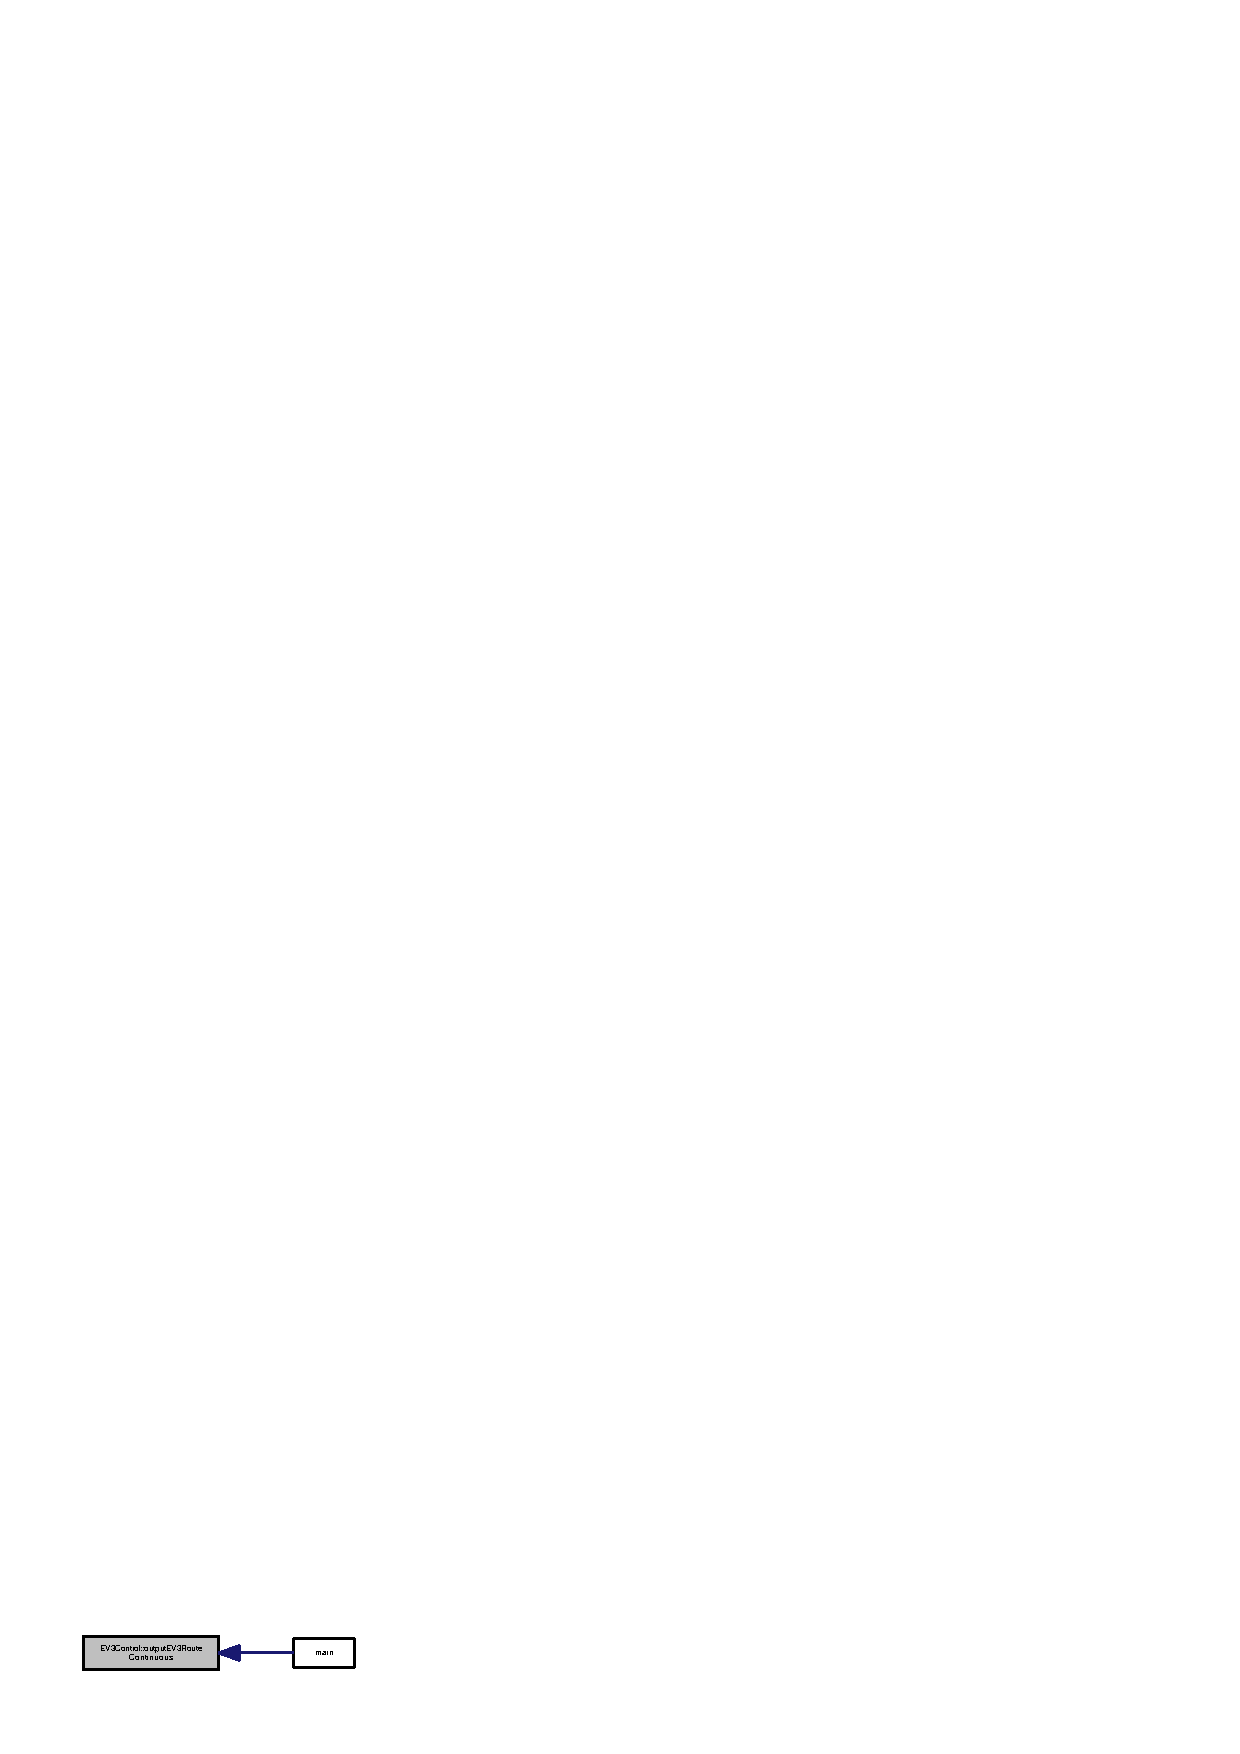
\includegraphics[width=174pt]{class_e_v3_control_a03d5b0e6707c302de24db329116f2142_icgraph}
\end{center}
\end{figure}


\index{E\-V3\-Control@{E\-V3\-Control}!set6\-Do\-F\-E\-V3@{set6\-Do\-F\-E\-V3}}
\index{set6\-Do\-F\-E\-V3@{set6\-Do\-F\-E\-V3}!EV3Control@{E\-V3\-Control}}
\subsubsection[{set6\-Do\-F\-E\-V3}]{\setlength{\rightskip}{0pt plus 5cm}void E\-V3\-Control\-::set6\-Do\-F\-E\-V3 (
\begin{DoxyParamCaption}
\item[{pcl\-::\-Point\-Cloud$<$ pcl\-::\-Point\-X\-Y\-Z\-R\-G\-B $>$\-::Ptr \&}]{input\-Point\-Cloud, }
\item[{Point3d}]{centroid, }
\item[{{\bf Attitude\-Angle}}]{attitude\-\_\-angle}
\end{DoxyParamCaption}
)}\label{class_e_v3_control_a8ef402279dc736292ae0cf780dd3aed8}


最小二乗法によって求めた平均座標と位置を\-E\-V3の制御のために構造体に格納する(c80) 

メソッド\-E\-V3\-Control\-::set6\-Do\-F\-E\-V3().最小二乗法によって求めた平均座標と位置を\-E\-V3の制御のために構造体に格納する


\begin{DoxyParams}{引数}
{\em \&input\-Point\-Cloud} & pcl\-::\-Point\-Cloud$<$pcl\-::\-Point\-X\-Y\-Z\-R\-G\-B$>$\-::\-Ptr型.入力するポイントクラウド \\
\hline
{\em centroid} & Point3d型.重心座標 \\
\hline
{\em attitude\-\_\-angle} & Attitude\-Angle型.姿勢角 \\
\hline
\end{DoxyParams}


 E\-V3\-Control.\-cpp の 49 行目に定義があります。



参照先 ev3\-\_\-6dof, Do\-F6i\-::pitch, Attitude\-Angle\-::pitch, Do\-F6i\-::roll, Attitude\-Angle\-::roll, Do\-F6i\-::x, Do\-F6i\-::y, Do\-F6i\-::yaw, Attitude\-Angle\-::yaw, Do\-F6i\-::z.



参照元 main().



被呼び出し関係図\-:\nopagebreak
\begin{figure}[H]
\begin{center}
\leavevmode
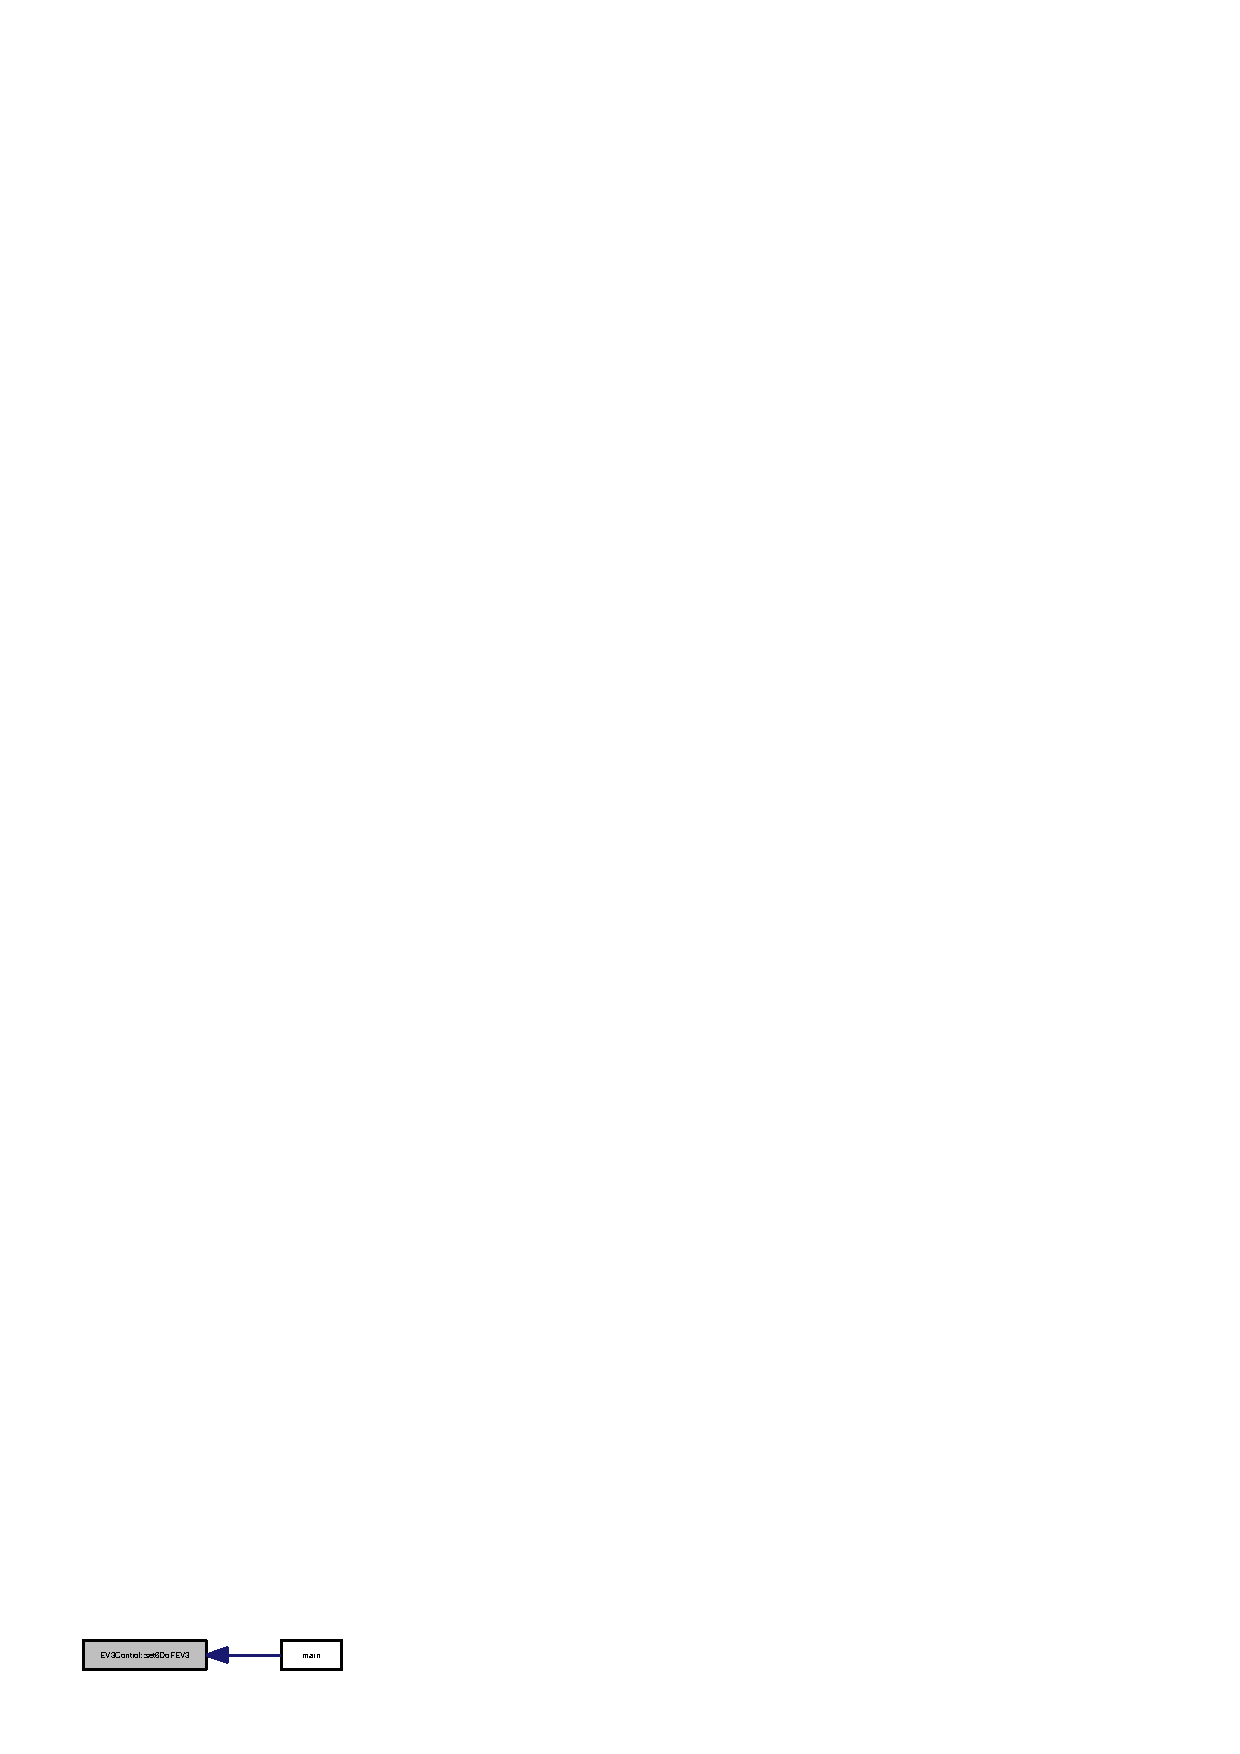
\includegraphics[width=168pt]{class_e_v3_control_a8ef402279dc736292ae0cf780dd3aed8_icgraph}
\end{center}
\end{figure}




\subsection{メンバ詳解}
\index{E\-V3\-Control@{E\-V3\-Control}!before@{before}}
\index{before@{before}!EV3Control@{E\-V3\-Control}}
\subsubsection[{before}]{\setlength{\rightskip}{0pt plus 5cm}{\bf Do\-F6i} E\-V3\-Control\-::before}\label{class_e_v3_control_aadcbe063497900efa4d94b3a46edb688}


前フレームの6\-Do\-F情報 



 E\-V3\-Control.\-hpp の 35 行目に定義があります。



参照元 E\-V3\-Control(), get\-Velocityin\-Sec().

\index{E\-V3\-Control@{E\-V3\-Control}!count\-\_\-average@{count\-\_\-average}}
\index{count\-\_\-average@{count\-\_\-average}!EV3Control@{E\-V3\-Control}}
\subsubsection[{count\-\_\-average}]{\setlength{\rightskip}{0pt plus 5cm}int E\-V3\-Control\-::count\-\_\-average}\label{class_e_v3_control_a094ccebd1c4d6b6432743fd7284ebea8}


速度とヨー角の過去5フレーム分の平均を取るために最初の5フレームをカウントするための変数 



 E\-V3\-Control.\-hpp の 42 行目に定義があります。



参照元 E\-V3\-Control(), get\-Average\-Velocity\-And\-Yaw().

\index{E\-V3\-Control@{E\-V3\-Control}!current@{current}}
\index{current@{current}!EV3Control@{E\-V3\-Control}}
\subsubsection[{current}]{\setlength{\rightskip}{0pt plus 5cm}{\bf Do\-F6i} E\-V3\-Control\-::current}\label{class_e_v3_control_a0407cbbddf22869f450b954d56c79c16}


現フレームの6\-Do\-F情報 



 E\-V3\-Control.\-hpp の 36 行目に定義があります。



参照元 E\-V3\-Control(), get\-Velocityin\-Sec().

\index{E\-V3\-Control@{E\-V3\-Control}!current\-\_\-average@{current\-\_\-average}}
\index{current\-\_\-average@{current\-\_\-average}!EV3Control@{E\-V3\-Control}}
\subsubsection[{current\-\_\-average}]{\setlength{\rightskip}{0pt plus 5cm}{\bf Control\-Paramd} E\-V3\-Control\-::current\-\_\-average}\label{class_e_v3_control_a506596061888dfd4afc965d20fed26a8}


現在の平均の速度とヨー角 



 E\-V3\-Control.\-hpp の 41 行目に定義があります。



参照元 E\-V3\-Control(), get\-Average\-Velocity\-And\-Yaw(), output\-Control\-Information().

\index{E\-V3\-Control@{E\-V3\-Control}!ev3\-\_\-6dof@{ev3\-\_\-6dof}}
\index{ev3\-\_\-6dof@{ev3\-\_\-6dof}!EV3Control@{E\-V3\-Control}}
\subsubsection[{ev3\-\_\-6dof}]{\setlength{\rightskip}{0pt plus 5cm}{\bf Do\-F6i} E\-V3\-Control\-::ev3\-\_\-6dof}\label{class_e_v3_control_adeff38f95194c020c3c1c5c3ef6bd994}


E\-V3の6自由度(c80) 



 E\-V3\-Control.\-hpp の 32 行目に定義があります。



参照元 get\-Average\-Velocity\-And\-Yaw(), get\-Velocityin\-Sec(), output6\-Do\-F(), output6\-Do\-F\-Continuous(), output\-E\-V3\-Route\-Continuous(), set6\-Do\-F\-E\-V3().

\index{E\-V3\-Control@{E\-V3\-Control}!flag\-\_\-average@{flag\-\_\-average}}
\index{flag\-\_\-average@{flag\-\_\-average}!EV3Control@{E\-V3\-Control}}
\subsubsection[{flag\-\_\-average}]{\setlength{\rightskip}{0pt plus 5cm}bool E\-V3\-Control\-::flag\-\_\-average}\label{class_e_v3_control_a07e70076fc9fb9085b55be1a3a7be187}


始めの5フレーム分用 



 E\-V3\-Control.\-hpp の 43 行目に定義があります。



参照元 E\-V3\-Control(), get\-Average\-Velocity\-And\-Yaw().

\index{E\-V3\-Control@{E\-V3\-Control}!flag\-\_\-velocity@{flag\-\_\-velocity}}
\index{flag\-\_\-velocity@{flag\-\_\-velocity}!EV3Control@{E\-V3\-Control}}
\subsubsection[{flag\-\_\-velocity}]{\setlength{\rightskip}{0pt plus 5cm}bool E\-V3\-Control\-::flag\-\_\-velocity}\label{class_e_v3_control_a353439722104f9c309920d0c0a1491de}


最初の1フレームのためのフラグ 



 E\-V3\-Control.\-hpp の 38 行目に定義があります。



参照元 E\-V3\-Control(), get\-Velocityin\-Sec().

\index{E\-V3\-Control@{E\-V3\-Control}!save\-\_\-flag@{save\-\_\-flag}}
\index{save\-\_\-flag@{save\-\_\-flag}!EV3Control@{E\-V3\-Control}}
\subsubsection[{save\-\_\-flag}]{\setlength{\rightskip}{0pt plus 5cm}bool E\-V3\-Control\-::save\-\_\-flag}\label{class_e_v3_control_abdd8dd38a39186e10013869fa4236605}


6\-Do\-F情報を出力するかチェックするためのフラグ 



 E\-V3\-Control.\-hpp の 48 行目に定義があります。



参照元 E\-V3\-Control(), main(), output6\-Do\-F\-Continuous().

\index{E\-V3\-Control@{E\-V3\-Control}!velocity@{velocity}}
\index{velocity@{velocity}!EV3Control@{E\-V3\-Control}}
\subsubsection[{velocity}]{\setlength{\rightskip}{0pt plus 5cm}double E\-V3\-Control\-::velocity}\label{class_e_v3_control_a3dbcb2b713381b2c050523b3a946af0a}


速度v(c85) 



 E\-V3\-Control.\-hpp の 37 行目に定義があります。



参照元 get\-Average\-Velocity\-And\-Yaw(), get\-Velocityin\-Sec().



このクラス詳解は次のファイルから抽出されました\-:\begin{DoxyCompactItemize}
\item 
{\bf E\-V3\-Control.\-hpp}\item 
{\bf E\-V3\-Control.\-cpp}\end{DoxyCompactItemize}

\section{Image\-Processing クラス}
\label{class_image_processing}\index{Image\-Processing@{Image\-Processing}}


画像処理用のクラス  




{\ttfamily \#include $<$Image\-Processing.\-hpp$>$}

\subsection*{公開メンバ関数}
\begin{DoxyCompactItemize}
\item 
{\bf Image\-Processing} ()
\begin{DoxyCompactList}\small\item\em コンストラクタ \end{DoxyCompactList}\item 
{\bf $\sim$\-Image\-Processing} ()
\begin{DoxyCompactList}\small\item\em デストラクタ \end{DoxyCompactList}\item 
void {\bf show\-Image} (string window\-Name, Mat \&input\-\_\-image)
\begin{DoxyCompactList}\small\item\em ウインドウの名前を引数に追加(c31).\-Matの表示(c17) \end{DoxyCompactList}\item 
void {\bf show\-Image\-Together} (Mat \&image1, Mat \&image2)
\begin{DoxyCompactList}\small\item\em 2つの画像を一緒に表示(c36) \end{DoxyCompactList}\item 
void {\bf show\-Image\-Together} (Mat \&image1, Mat \&image2, Mat \&image3)
\begin{DoxyCompactList}\small\item\em 3つの画像を一緒に表示(c36) \end{DoxyCompactList}\item 
void {\bf load\-Internal\-Camera\-Parameter} (const string camera\-Param\-File)
\begin{DoxyCompactList}\small\item\em カメラキャリブレーションによって得られたパラメータを適用する(c54) \end{DoxyCompactList}\item 
Mat {\bf get\-Undistortion\-Image} (Mat \&input\-Original\-Image)
\begin{DoxyCompactList}\small\item\em キャリブレーションデータを用いて\-Kinectから取得した画像を補正する(c71) \end{DoxyCompactList}\item 
Mat {\bf get\-Background\-Substraction\-Bin\-Image} (Mat \&current\-\_\-image, Mat \&backgound\-\_\-gray\-\_\-image)
\begin{DoxyCompactList}\small\item\em 背景差分によって得られた二値画像(c75) \end{DoxyCompactList}\item 
void {\bf open\-C\-V\-Setting\-Trackbar} (const string trackbar\-\_\-name)
\begin{DoxyCompactList}\small\item\em 画像処理関連のトラックバーを表示するメソッド \end{DoxyCompactList}\item 
Mat {\bf get\-Unit\-Mask} (Mat \&input\-\_\-binimage)
\begin{DoxyCompactList}\small\item\em E\-V3のユニット部のみのマスク画像を取得するメソッド \end{DoxyCompactList}\item 
void {\bf output\-Image\-Select\-Directory} (int save\-\_\-count, char $\ast$original\-\_\-dirpath, char $\ast$save\-\_\-filename, Mat \&output\-\_\-image)
\begin{DoxyCompactList}\small\item\em メソッド\-Image\-Processing\-::output\-Image\-Select\-Directory().出力したディレクトリにファイルを出力するメソッド \end{DoxyCompactList}\end{DoxyCompactItemize}
\subsection*{公開変数類}
\begin{DoxyCompactItemize}
\item 
int {\bf th}
\begin{DoxyCompactList}\small\item\em 二値化するときの閾値(c82) \end{DoxyCompactList}\item 
int {\bf neighborhood}
\begin{DoxyCompactList}\small\item\em 平滑化を行うときの近傍 \end{DoxyCompactList}\item 
int {\bf closing\-\_\-times}
\begin{DoxyCompactList}\small\item\em クロージングを行う回数 \end{DoxyCompactList}\end{DoxyCompactItemize}


\subsection{詳解}
画像処理用のクラス 

 Image\-Processing.\-hpp の 19 行目に定義があります。



\subsection{構築子と解体子}
\index{Image\-Processing@{Image\-Processing}!Image\-Processing@{Image\-Processing}}
\index{Image\-Processing@{Image\-Processing}!ImageProcessing@{Image\-Processing}}
\subsubsection[{Image\-Processing}]{\setlength{\rightskip}{0pt plus 5cm}Image\-Processing\-::\-Image\-Processing (
\begin{DoxyParamCaption}
{}
\end{DoxyParamCaption}
)}\label{class_image_processing_a0090ffe36a912d6df5d7a1f507f6252e}


コンストラクタ 

メソッド\-Image\-Processing\-::\-Image\-Processing().コンストラクタ 

 Image\-Processing.\-cpp の 15 行目に定義があります。



参照先 closing\-\_\-times, neighborhood, th.

\index{Image\-Processing@{Image\-Processing}!$\sim$\-Image\-Processing@{$\sim$\-Image\-Processing}}
\index{$\sim$\-Image\-Processing@{$\sim$\-Image\-Processing}!ImageProcessing@{Image\-Processing}}
\subsubsection[{$\sim$\-Image\-Processing}]{\setlength{\rightskip}{0pt plus 5cm}Image\-Processing\-::$\sim$\-Image\-Processing (
\begin{DoxyParamCaption}
{}
\end{DoxyParamCaption}
)}\label{class_image_processing_a1d4bd00ec1862112552c663034cebabc}


デストラクタ 

メソッド\-Image\-Processing\-::$\sim$\-Image\-Processing().デストラクタ 

 Image\-Processing.\-cpp の 26 行目に定義があります。



\subsection{関数詳解}
\index{Image\-Processing@{Image\-Processing}!get\-Background\-Substraction\-Bin\-Image@{get\-Background\-Substraction\-Bin\-Image}}
\index{get\-Background\-Substraction\-Bin\-Image@{get\-Background\-Substraction\-Bin\-Image}!ImageProcessing@{Image\-Processing}}
\subsubsection[{get\-Background\-Substraction\-Bin\-Image}]{\setlength{\rightskip}{0pt plus 5cm}Mat Image\-Processing\-::get\-Background\-Substraction\-Bin\-Image (
\begin{DoxyParamCaption}
\item[{Mat \&}]{current\-\_\-image, }
\item[{Mat \&}]{background\-\_\-gray\-\_\-image}
\end{DoxyParamCaption}
)}\label{class_image_processing_ae7dc0c506adedb62687e15f0a1b1c7f0}


背景差分によって得られた二値画像(c75) 

メソッド\-Image\-Processing\-::get\-Background\-Substraction\-Bin\-Image().背景差分によって得られた二値画像(c75)


\begin{DoxyParams}{引数}
{\em \&current\-\_\-image} & cv\-::\-Mat型.現フレームの入力画像 \\
\hline
{\em \&background\-\_\-image} & cv\-::\-Mat型.背景画像の入力 \\
\hline
\end{DoxyParams}
\begin{DoxyReturn}{戻り値}
closing\-\_\-image cv\-::\-Mat型.出力画像 
\end{DoxyReturn}
$<$現在のグレースケール画像(c75)

$<$背景差分画像(c74)

$<$背景差分画像の二値画像(c75)

$<$背景差分画像の二値画像を平滑化したもの(c75)

$<$クロージング処理御用変数 

 Image\-Processing.\-cpp の 130 行目に定義があります。



参照先 closing\-\_\-times, neighborhood, th.



参照元 main().



被呼び出し関係図\-:\nopagebreak
\begin{figure}[H]
\begin{center}
\leavevmode
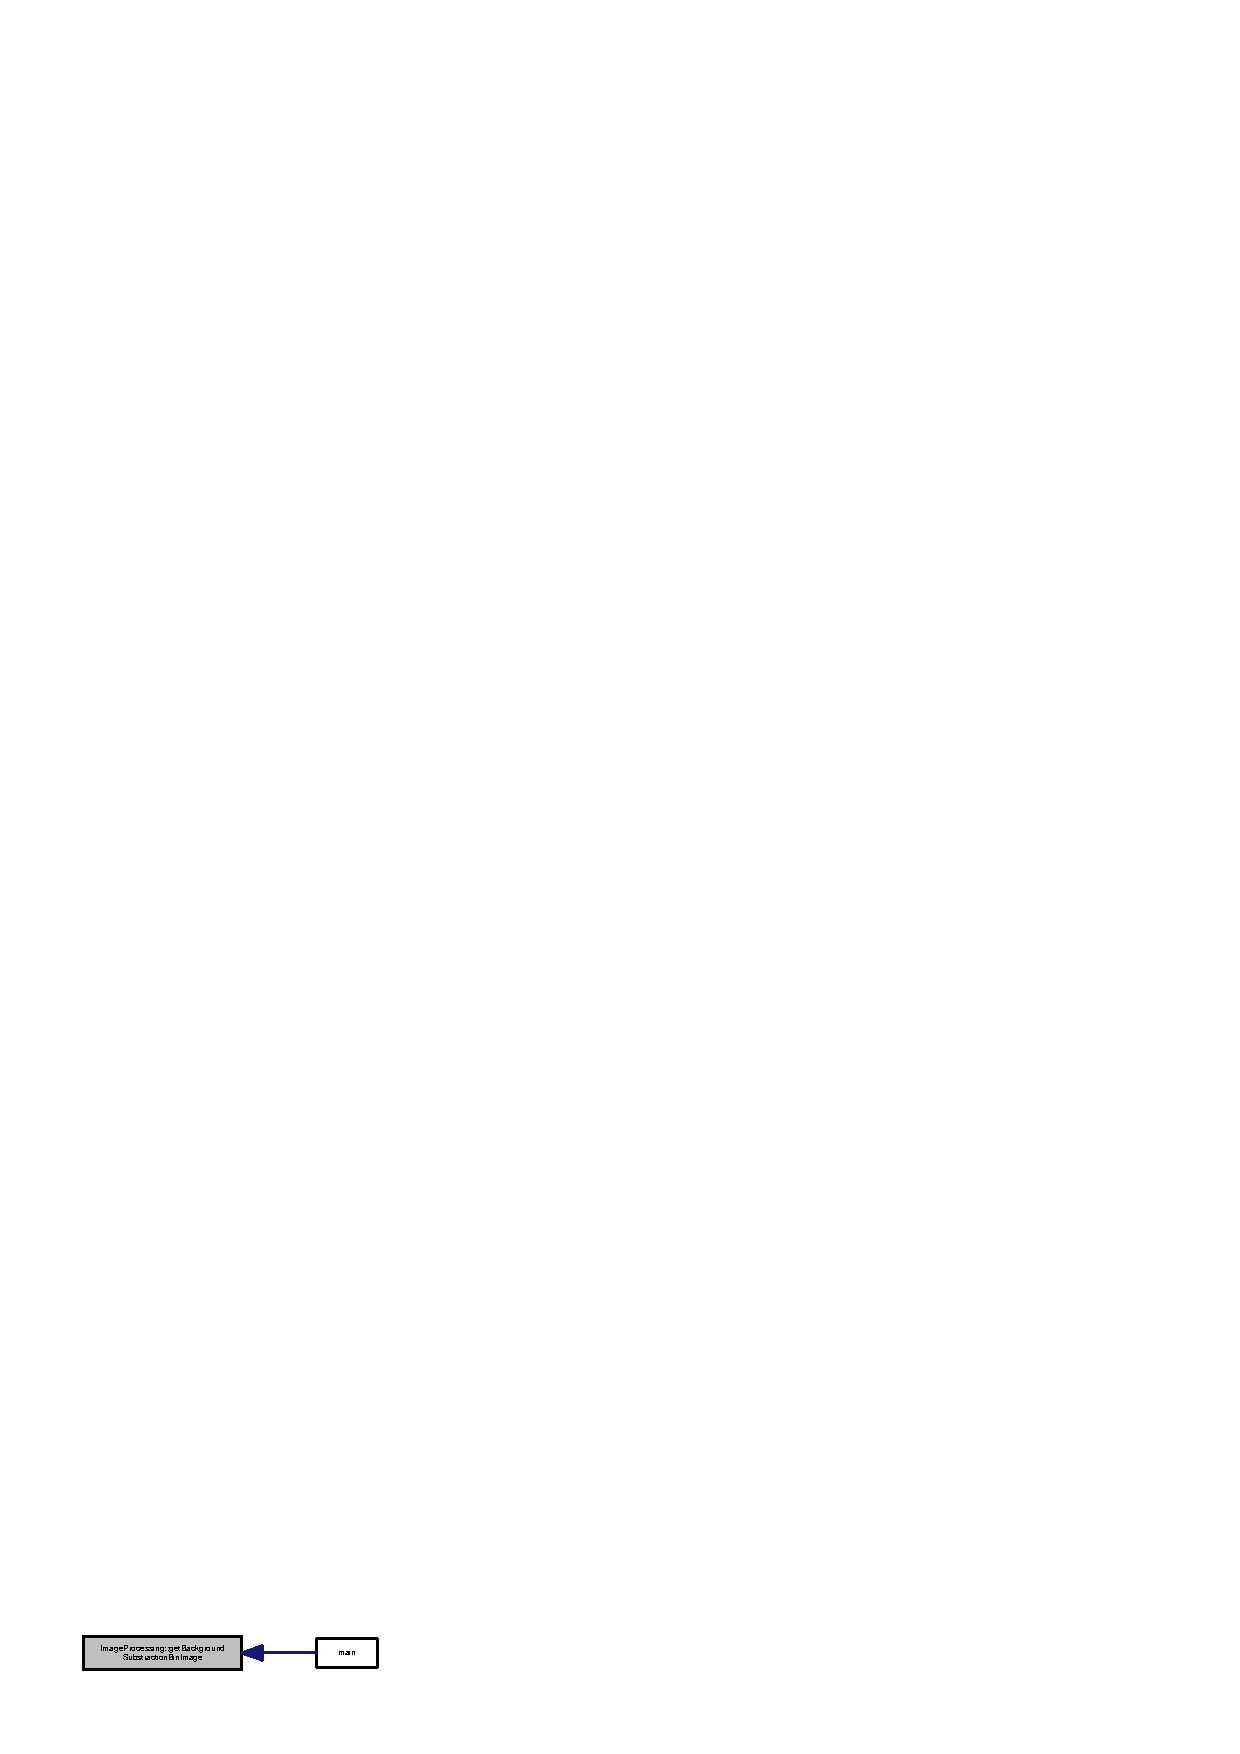
\includegraphics[width=185pt]{class_image_processing_ae7dc0c506adedb62687e15f0a1b1c7f0_icgraph}
\end{center}
\end{figure}


\index{Image\-Processing@{Image\-Processing}!get\-Undistortion\-Image@{get\-Undistortion\-Image}}
\index{get\-Undistortion\-Image@{get\-Undistortion\-Image}!ImageProcessing@{Image\-Processing}}
\subsubsection[{get\-Undistortion\-Image}]{\setlength{\rightskip}{0pt plus 5cm}Mat Image\-Processing\-::get\-Undistortion\-Image (
\begin{DoxyParamCaption}
\item[{Mat \&}]{input\-Original\-Image}
\end{DoxyParamCaption}
)}\label{class_image_processing_a5fa5bf016a9d7f946919d0a34a47031c}


キャリブレーションデータを用いて\-Kinectから取得した画像を補正する(c71) 

メソッド\-Image\-Processing\-::get\-Undistortion\-Image().キャリブレーションデータを用いて\-Kinectから取得した画像を補正する


\begin{DoxyParams}{引数}
{\em \&input\-Original\-Image} & cv\-::\-Mat型.キャリブレーションを行いたい入力画像 \\
\hline
\end{DoxyParams}
\begin{DoxyReturn}{戻り値}
undistortion\-Image cv\-::\-Mat型.キャリブレーション後の画像 
\end{DoxyReturn}


 Image\-Processing.\-cpp の 115 行目に定義があります。



参照元 main().



被呼び出し関係図\-:\nopagebreak
\begin{figure}[H]
\begin{center}
\leavevmode
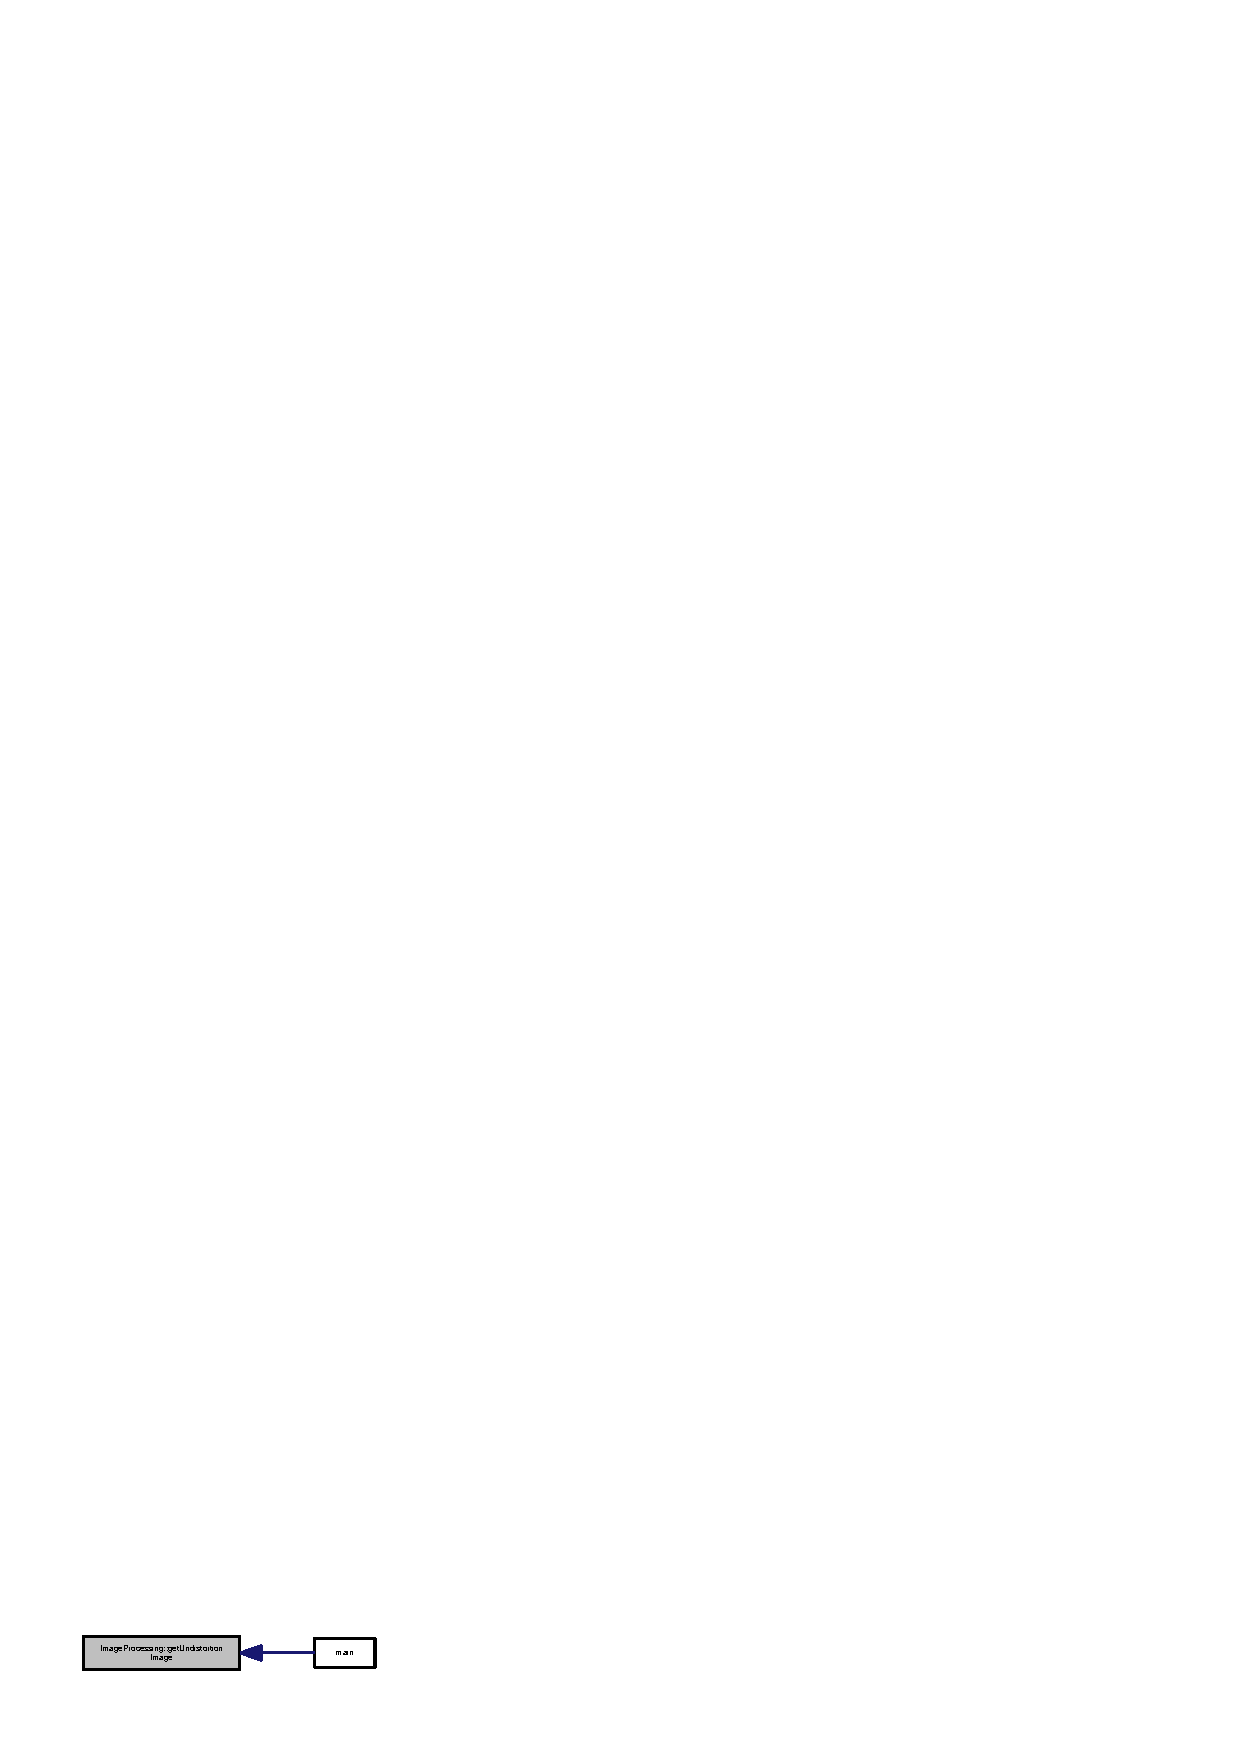
\includegraphics[width=184pt]{class_image_processing_a5fa5bf016a9d7f946919d0a34a47031c_icgraph}
\end{center}
\end{figure}


\index{Image\-Processing@{Image\-Processing}!get\-Unit\-Mask@{get\-Unit\-Mask}}
\index{get\-Unit\-Mask@{get\-Unit\-Mask}!ImageProcessing@{Image\-Processing}}
\subsubsection[{get\-Unit\-Mask}]{\setlength{\rightskip}{0pt plus 5cm}Mat Image\-Processing\-::get\-Unit\-Mask (
\begin{DoxyParamCaption}
\item[{Mat \&}]{input\-\_\-binimage}
\end{DoxyParamCaption}
)}\label{class_image_processing_a691c472c29caaab27924bd469a2ea1f1}


E\-V3のユニット部のみのマスク画像を取得するメソッド 

メソッド\-Image\-Processing\-::get\-Unit\-Mask().\-E\-V3のユニット部のみのマスク画像を取得するメソッド


\begin{DoxyParams}{引数}
{\em \&input\-\_\-binimage} & cv\-::\-Mat型.入力画像(二値画像) \\
\hline
\end{DoxyParams}
\begin{DoxyReturn}{戻り値}
input\-\_\-binimage cv\-::\-Mat型.出力画像(マスク処理された二値画像) 
\end{DoxyReturn}


 Image\-Processing.\-cpp の 171 行目に定義があります。

\index{Image\-Processing@{Image\-Processing}!load\-Internal\-Camera\-Parameter@{load\-Internal\-Camera\-Parameter}}
\index{load\-Internal\-Camera\-Parameter@{load\-Internal\-Camera\-Parameter}!ImageProcessing@{Image\-Processing}}
\subsubsection[{load\-Internal\-Camera\-Parameter}]{\setlength{\rightskip}{0pt plus 5cm}void Image\-Processing\-::load\-Internal\-Camera\-Parameter (
\begin{DoxyParamCaption}
\item[{const string}]{camera\-Param\-File}
\end{DoxyParamCaption}
)}\label{class_image_processing_a58862a0cb31373a4d1a9d6a89fdd8e6c}


カメラキャリブレーションによって得られたパラメータを適用する(c54) 

Image\-Processing\-::load\-Internal\-Camera\-Param().カメラキャリブレーションによって得られたカメラパラメータを適用するメソッド(c54)


\begin{DoxyParams}{引数}
{\em camera\-Param\-File} & const string型.入力したいカメラパラメータのファイル名 \\
\hline
\end{DoxyParams}


 Image\-Processing.\-cpp の 98 行目に定義があります。



参照元 main().



被呼び出し関係図\-:\nopagebreak
\begin{figure}[H]
\begin{center}
\leavevmode
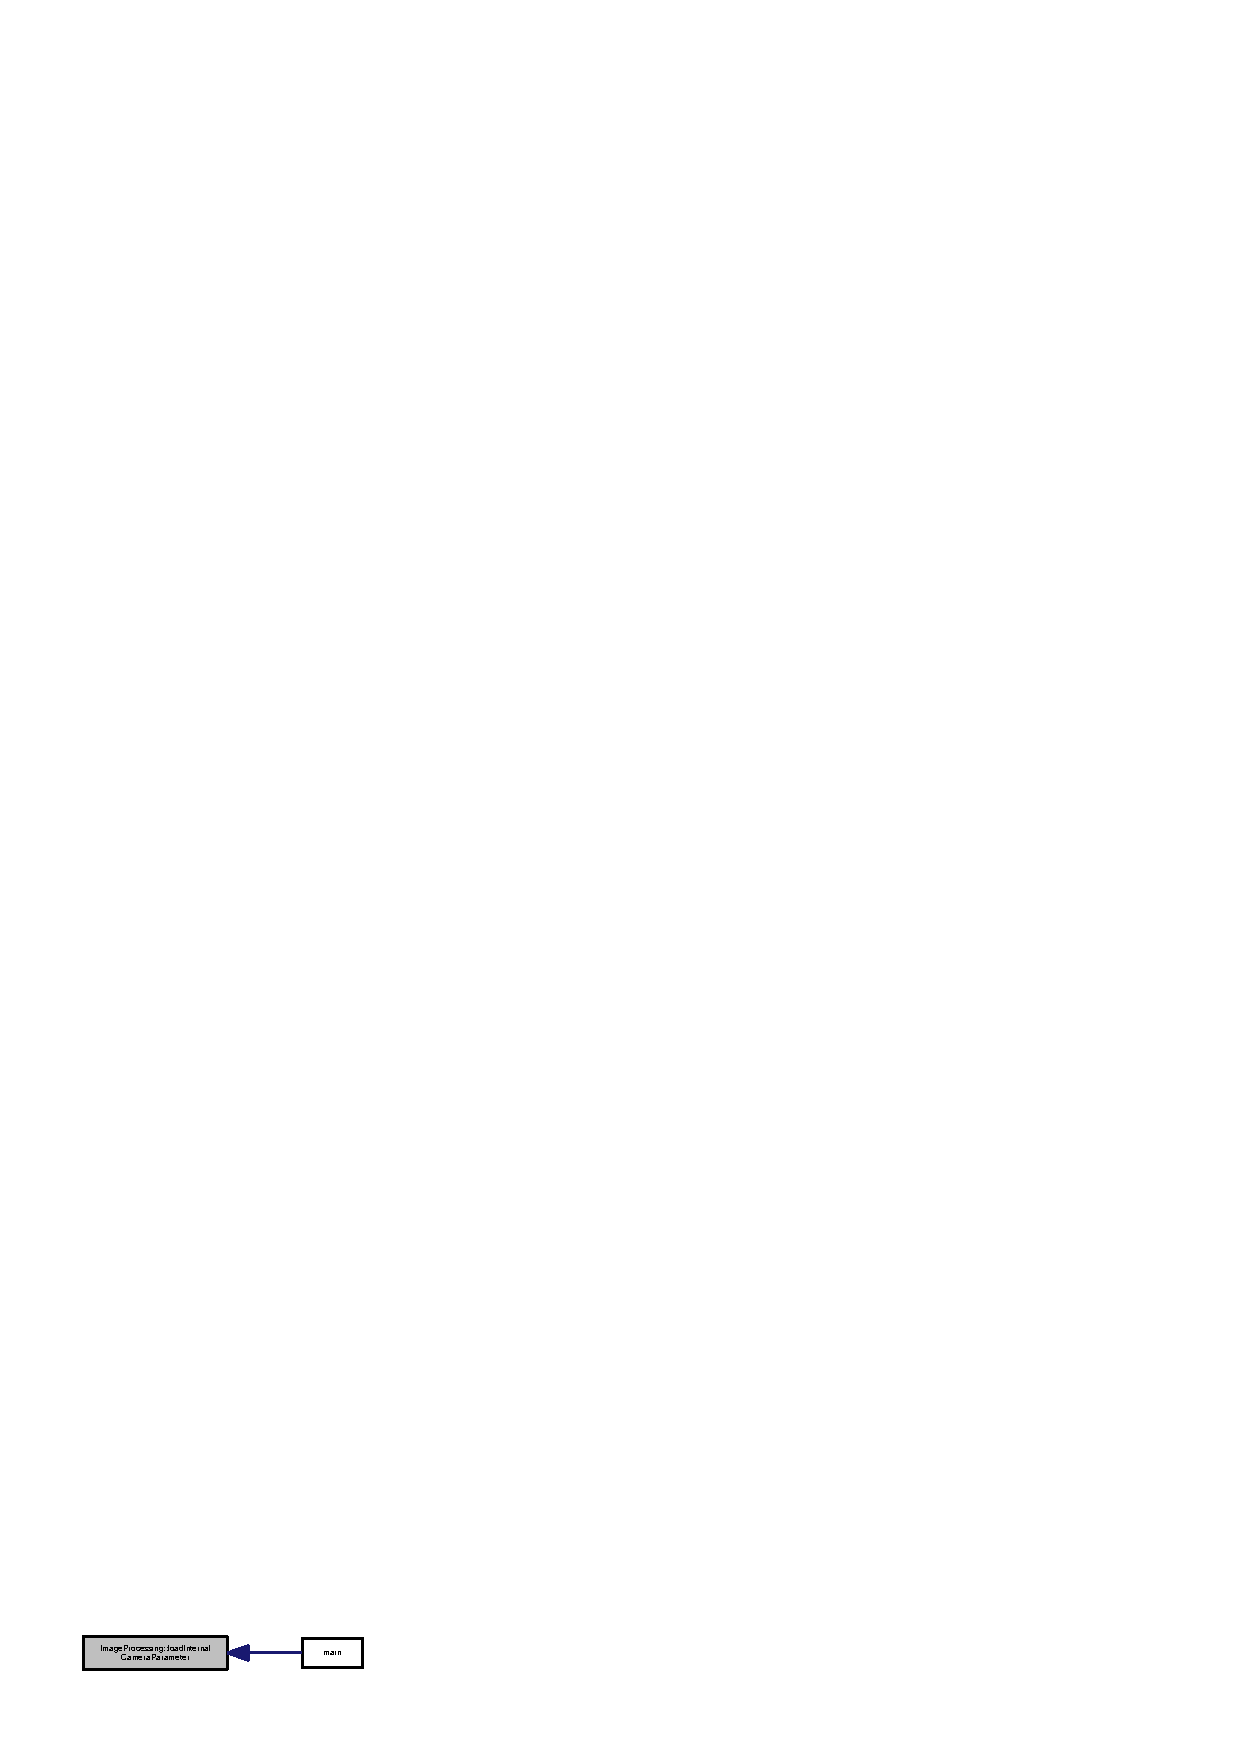
\includegraphics[width=178pt]{class_image_processing_a58862a0cb31373a4d1a9d6a89fdd8e6c_icgraph}
\end{center}
\end{figure}


\index{Image\-Processing@{Image\-Processing}!open\-C\-V\-Setting\-Trackbar@{open\-C\-V\-Setting\-Trackbar}}
\index{open\-C\-V\-Setting\-Trackbar@{open\-C\-V\-Setting\-Trackbar}!ImageProcessing@{Image\-Processing}}
\subsubsection[{open\-C\-V\-Setting\-Trackbar}]{\setlength{\rightskip}{0pt plus 5cm}void Image\-Processing\-::open\-C\-V\-Setting\-Trackbar (
\begin{DoxyParamCaption}
\item[{const string}]{trackbar\-\_\-name}
\end{DoxyParamCaption}
)}\label{class_image_processing_a36d146288e958736fd803fde49c064af}


画像処理関連のトラックバーを表示するメソッド 

メソッド\-Image\-Processing\-::open\-C\-V\-Setting\-Trackbar().\-Open\-C\-Vのトラックバーを表示するメソッド


\begin{DoxyParams}{引数}
{\em trackbar\-\_\-name} & const string型.\-Open\-C\-Vでマスク画像を設定するためのトラックバー名 \\
\hline
\end{DoxyParams}


 Image\-Processing.\-cpp の 156 行目に定義があります。



参照先 closing\-\_\-times, neighborhood, th.



参照元 main().



被呼び出し関係図\-:\nopagebreak
\begin{figure}[H]
\begin{center}
\leavevmode
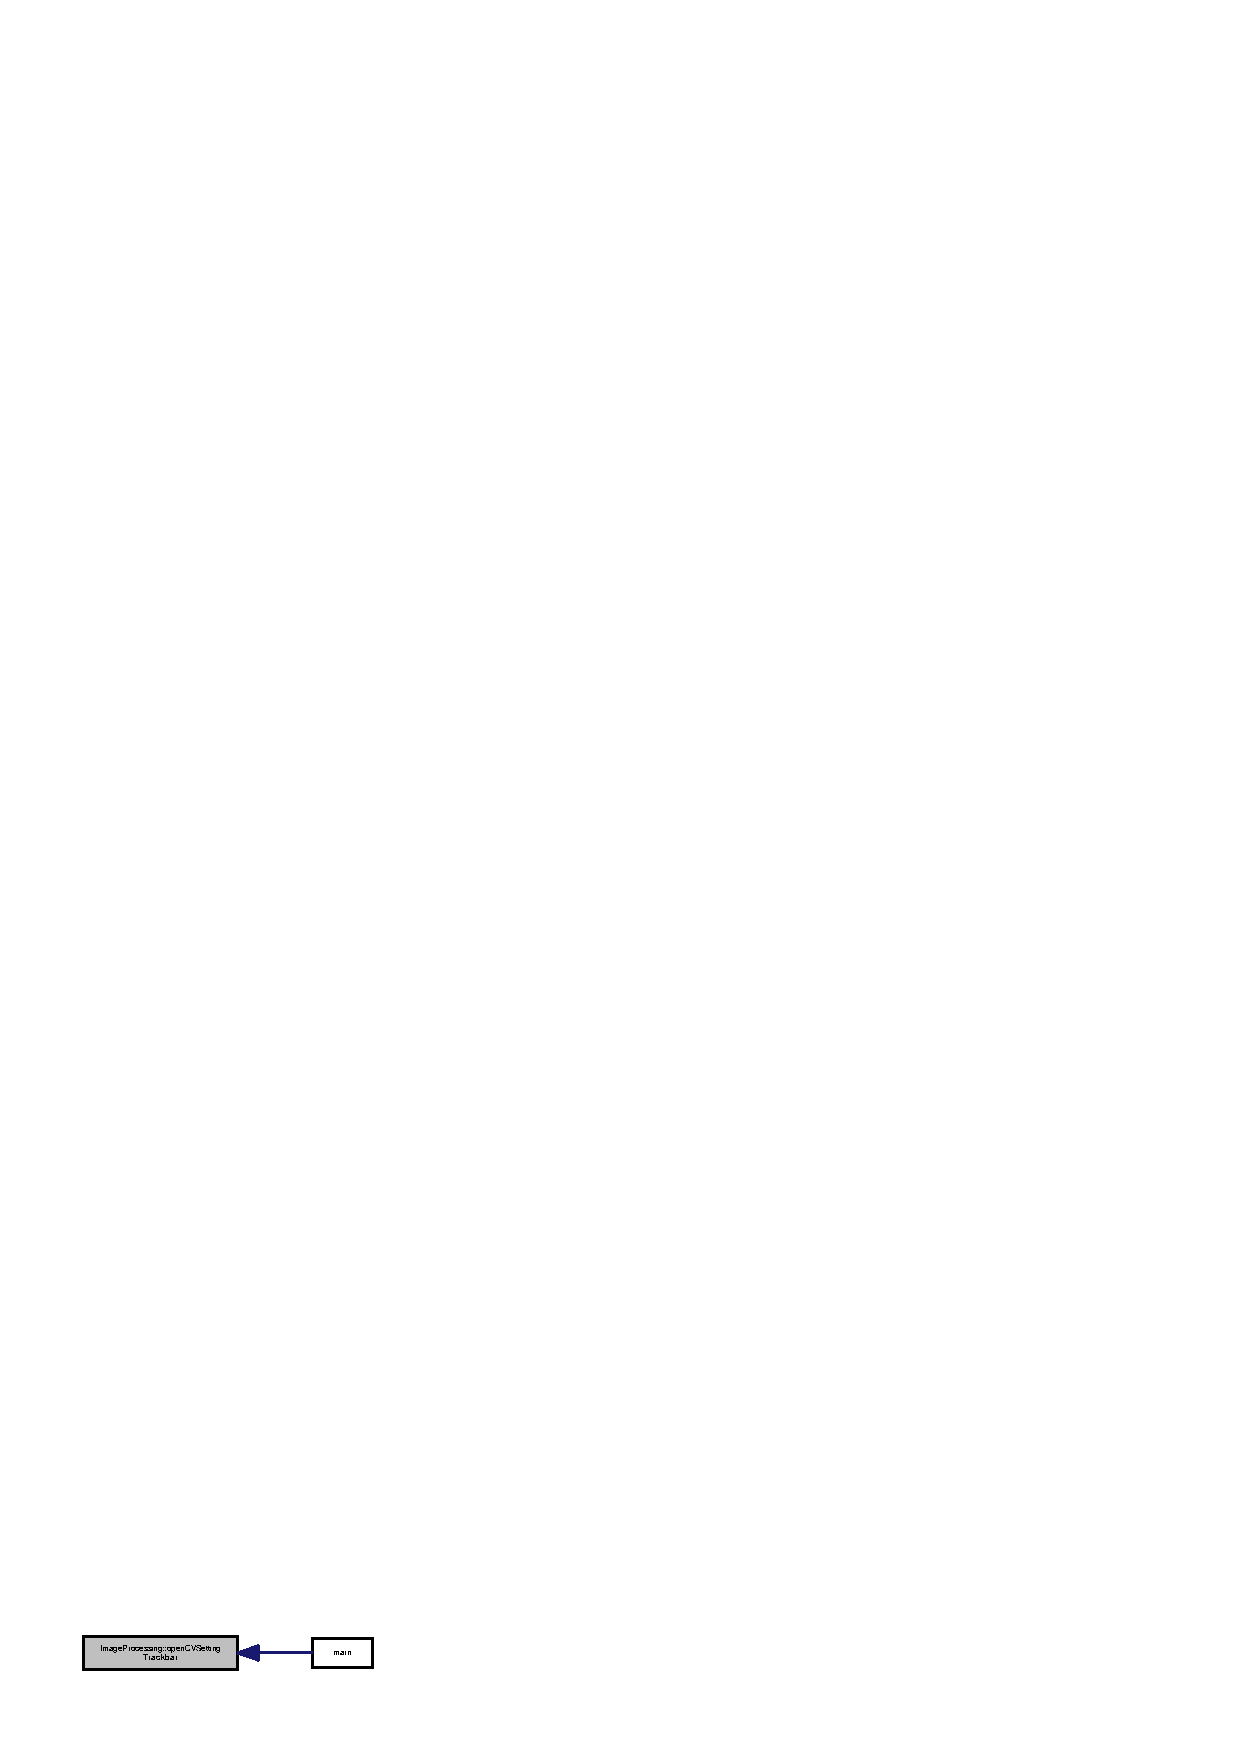
\includegraphics[width=183pt]{class_image_processing_a36d146288e958736fd803fde49c064af_icgraph}
\end{center}
\end{figure}


\index{Image\-Processing@{Image\-Processing}!output\-Image\-Select\-Directory@{output\-Image\-Select\-Directory}}
\index{output\-Image\-Select\-Directory@{output\-Image\-Select\-Directory}!ImageProcessing@{Image\-Processing}}
\subsubsection[{output\-Image\-Select\-Directory}]{\setlength{\rightskip}{0pt plus 5cm}void Image\-Processing\-::output\-Image\-Select\-Directory (
\begin{DoxyParamCaption}
\item[{int}]{save\-\_\-count, }
\item[{char $\ast$}]{original\-\_\-dirpath, }
\item[{char $\ast$}]{save\-\_\-filename, }
\item[{Mat \&}]{output\-\_\-image}
\end{DoxyParamCaption}
)}\label{class_image_processing_ac2a3a10ecc09a2be23b2cc673cee1e0c}


メソッド\-Image\-Processing\-::output\-Image\-Select\-Directory().出力したディレクトリにファイルを出力するメソッド 


\begin{DoxyParams}{引数}
{\em save\-\_\-count} & int型.保存数のカウント \\
\hline
{\em original\-\_\-dirpath} & char$\ast$型.基となるディレクトリ名 \\
\hline
{\em save\-\_\-filename} & char$\ast$.出力するファイル名 \\
\hline
{\em \&output\-\_\-image} & cv\-::\-Mat型.出力する画像 \\
\hline
\end{DoxyParams}


 Image\-Processing.\-cpp の 266 行目に定義があります。



参照先 N\-O\-C.



参照元 main().



被呼び出し関係図\-:\nopagebreak
\begin{figure}[H]
\begin{center}
\leavevmode
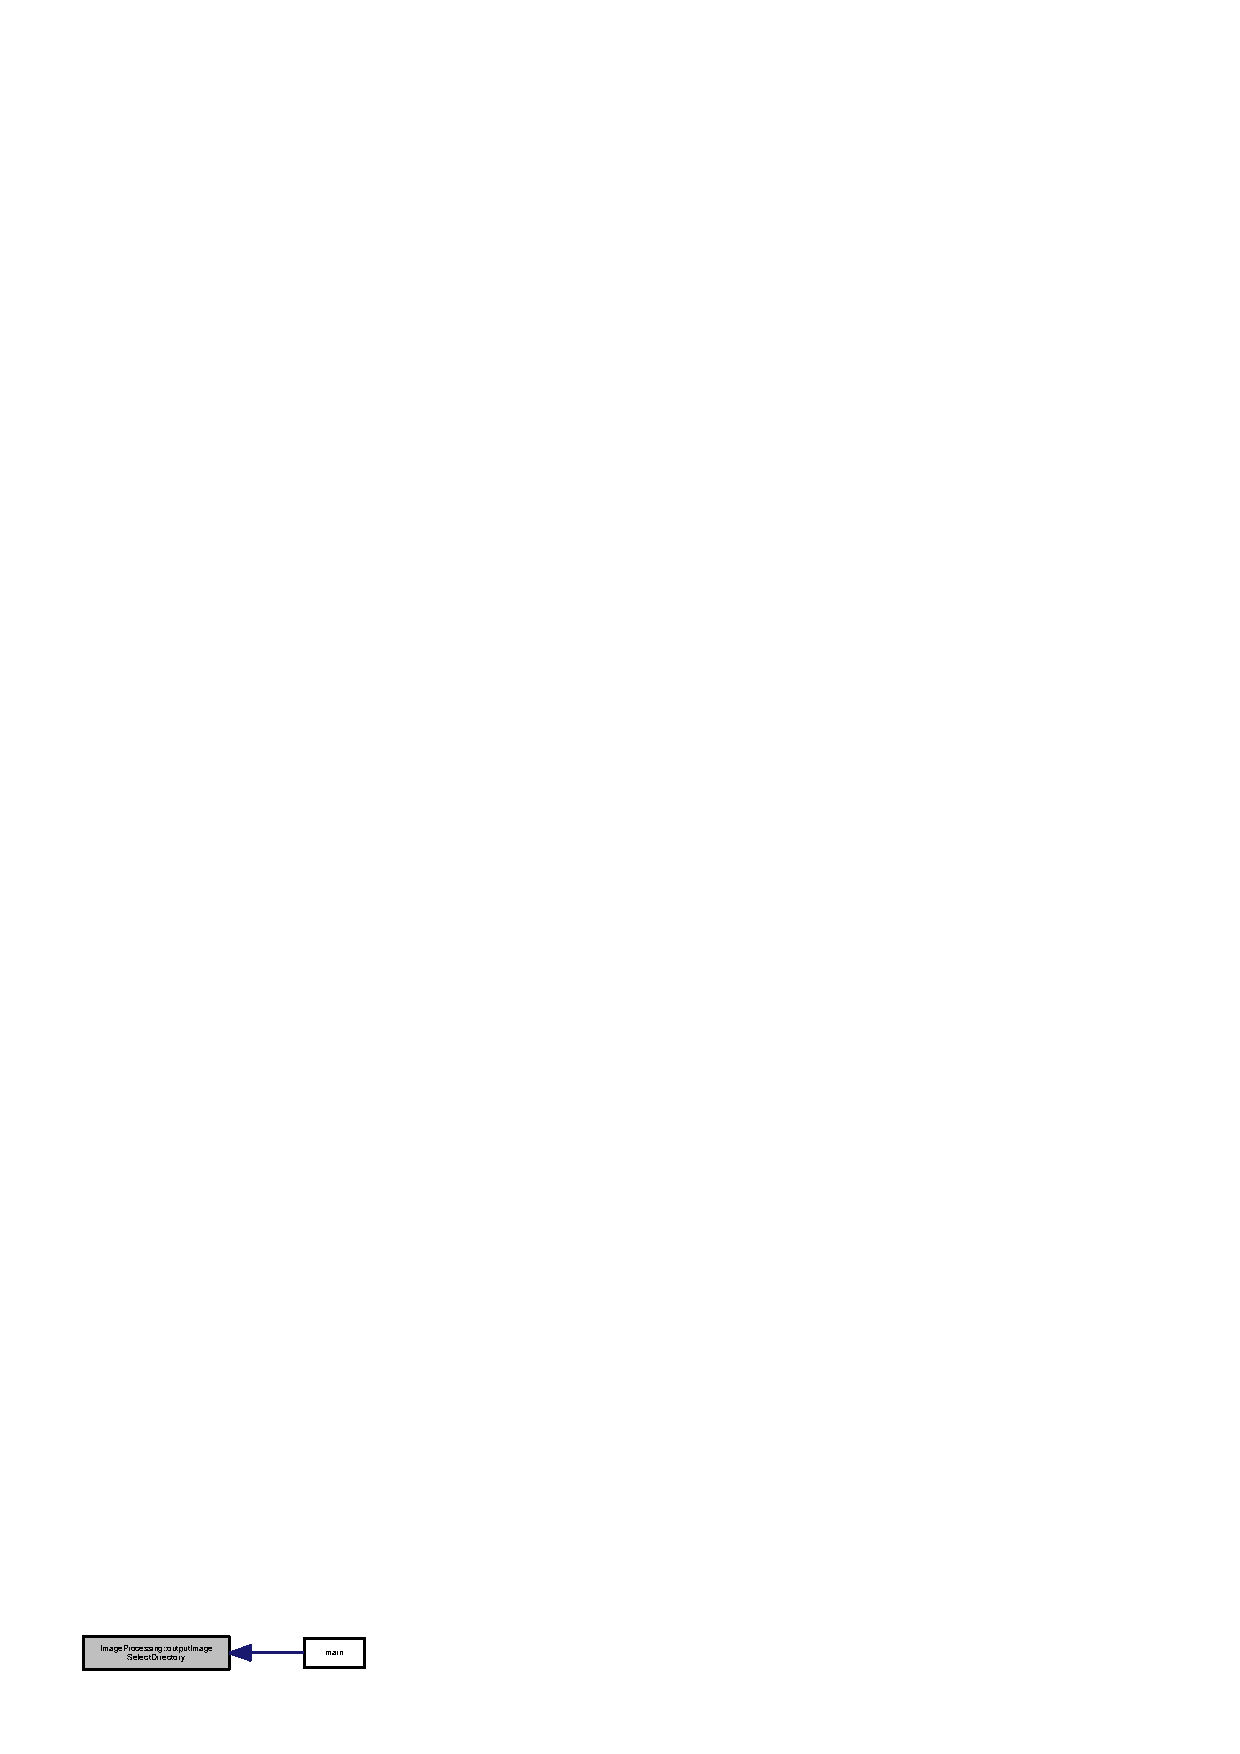
\includegraphics[width=179pt]{class_image_processing_ac2a3a10ecc09a2be23b2cc673cee1e0c_icgraph}
\end{center}
\end{figure}


\index{Image\-Processing@{Image\-Processing}!show\-Image@{show\-Image}}
\index{show\-Image@{show\-Image}!ImageProcessing@{Image\-Processing}}
\subsubsection[{show\-Image}]{\setlength{\rightskip}{0pt plus 5cm}void Image\-Processing\-::show\-Image (
\begin{DoxyParamCaption}
\item[{string}]{window\-Name, }
\item[{Mat \&}]{input\-\_\-image}
\end{DoxyParamCaption}
)}\label{class_image_processing_a77b6912e1d1182d29a7c8a8c639bb685}


ウインドウの名前を引数に追加(c31).\-Matの表示(c17) 

メソッド\-Image\-Processing\-::show\-Image().cv\-::\-Matを表示


\begin{DoxyParams}{引数}
{\em window\-Name} & std\-::string型.表示するウインドウ名 \\
\hline
{\em \&input\-\_\-image} & cv\-::\-Mat型.入力画像 \\
\hline
\end{DoxyParams}


 Image\-Processing.\-cpp の 36 行目に定義があります。



参照元 main(), show\-Image\-Together().



被呼び出し関係図\-:\nopagebreak
\begin{figure}[H]
\begin{center}
\leavevmode
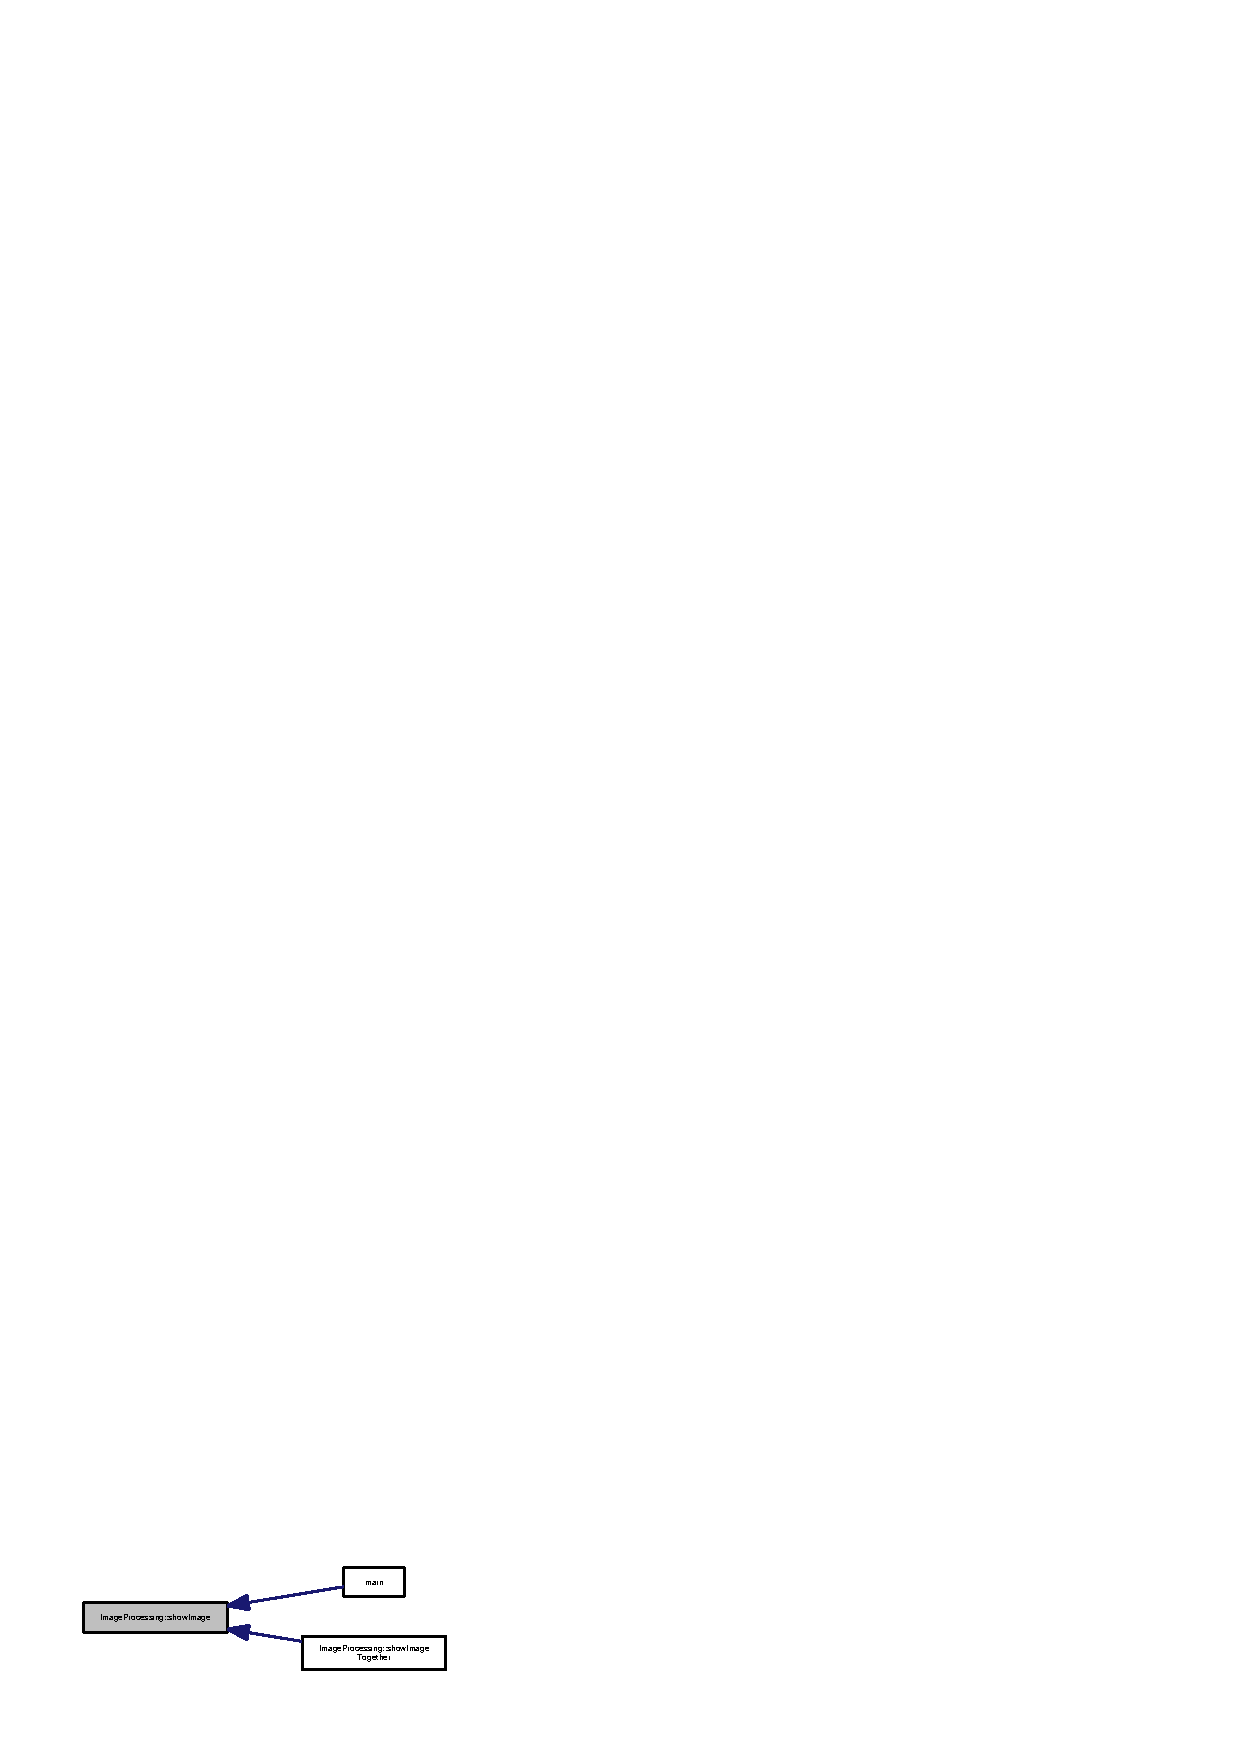
\includegraphics[width=218pt]{class_image_processing_a77b6912e1d1182d29a7c8a8c639bb685_icgraph}
\end{center}
\end{figure}


\index{Image\-Processing@{Image\-Processing}!show\-Image\-Together@{show\-Image\-Together}}
\index{show\-Image\-Together@{show\-Image\-Together}!ImageProcessing@{Image\-Processing}}
\subsubsection[{show\-Image\-Together}]{\setlength{\rightskip}{0pt plus 5cm}void Image\-Processing\-::show\-Image\-Together (
\begin{DoxyParamCaption}
\item[{Mat \&}]{image1, }
\item[{Mat \&}]{image2}
\end{DoxyParamCaption}
)}\label{class_image_processing_aece5b6cebfe47d9f65ce589168686189}


2つの画像を一緒に表示(c36) 

メソッド\-Image\-Processing\-::show\-Together\-Image().2つのcv\-::\-Matを1つのウインドウに表示


\begin{DoxyParams}{引数}
{\em \&image1} & cv\-::\-Mat型.入力画像1 \\
\hline
{\em \&image2} & cv\-::\-Mat型.入力画像2 \\
\hline
\end{DoxyParams}


 Image\-Processing.\-cpp の 48 行目に定義があります。



参照先 show\-Image().



呼び出し関係図\-:\nopagebreak
\begin{figure}[H]
\begin{center}
\leavevmode
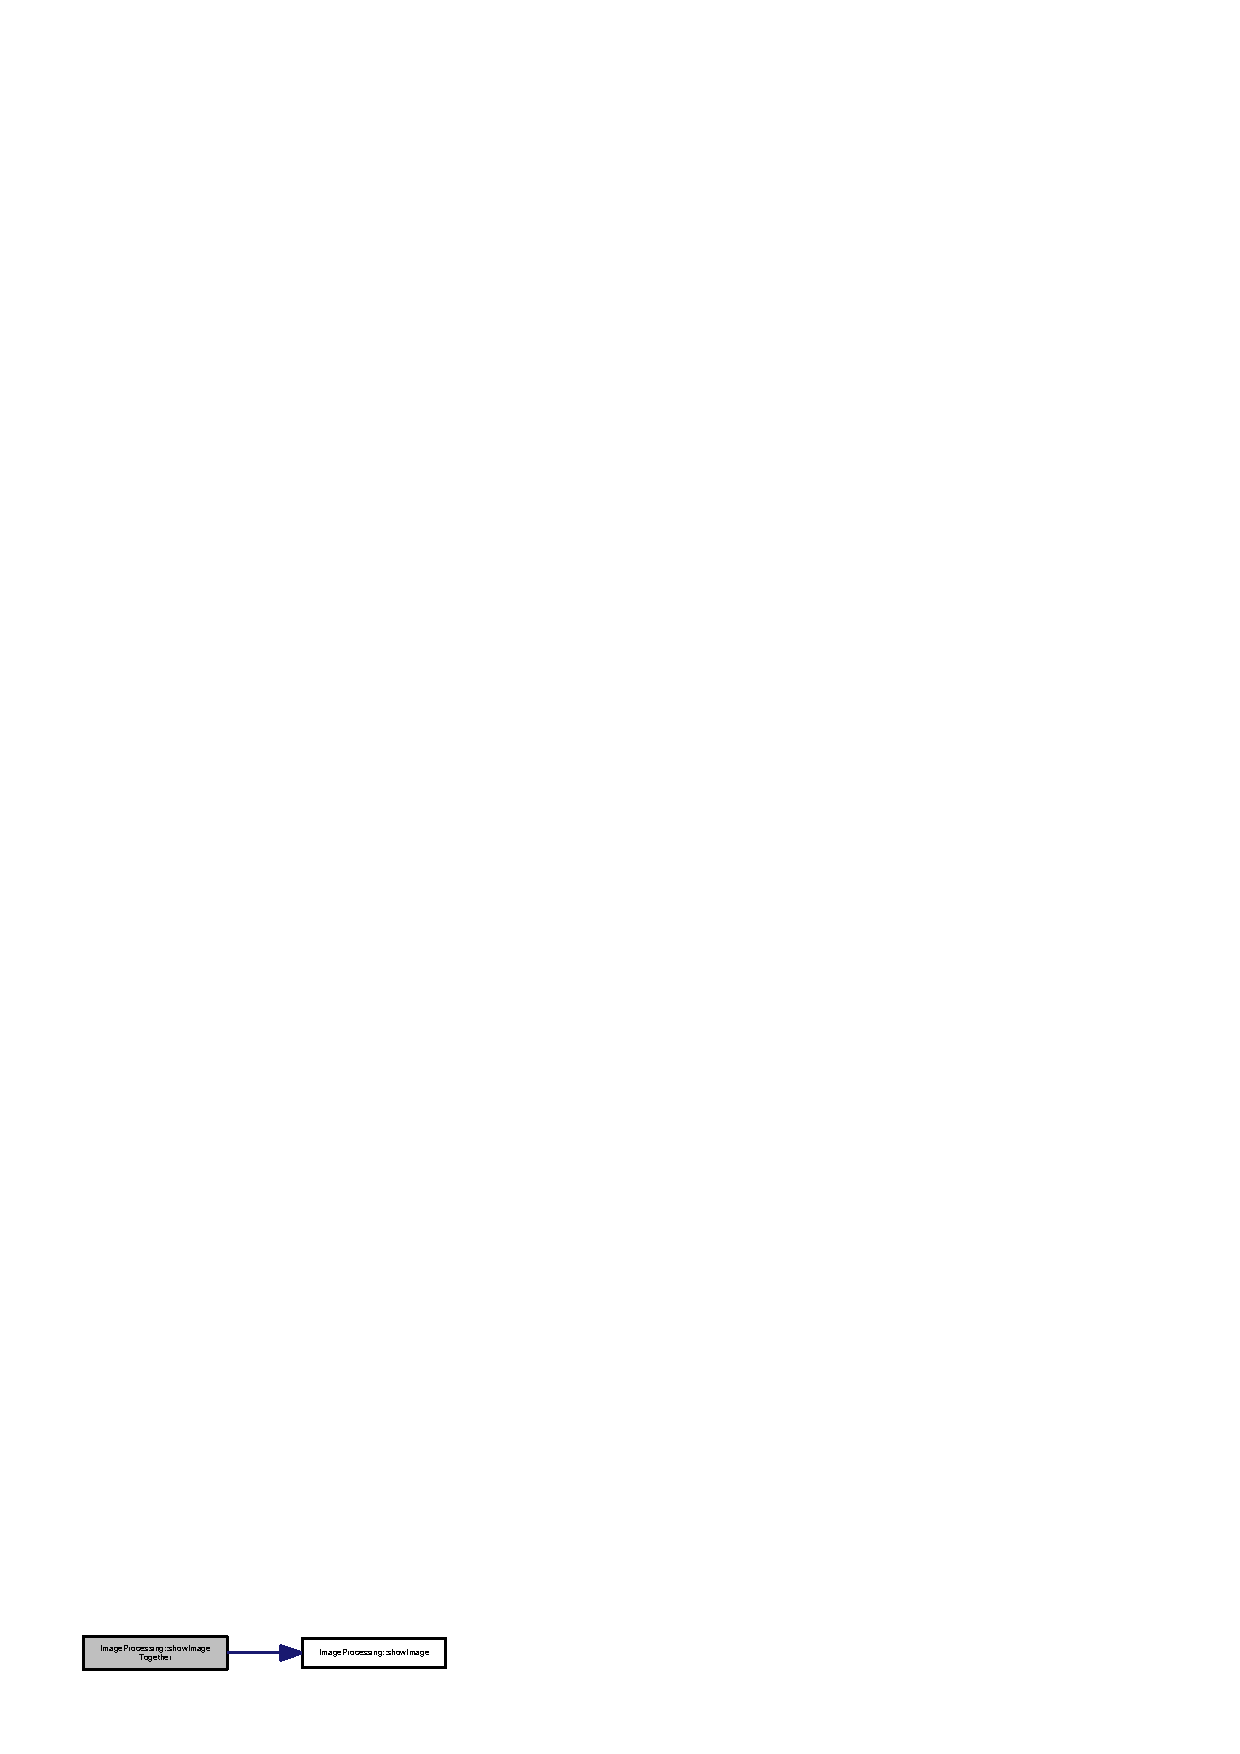
\includegraphics[width=218pt]{class_image_processing_aece5b6cebfe47d9f65ce589168686189_cgraph}
\end{center}
\end{figure}


\index{Image\-Processing@{Image\-Processing}!show\-Image\-Together@{show\-Image\-Together}}
\index{show\-Image\-Together@{show\-Image\-Together}!ImageProcessing@{Image\-Processing}}
\subsubsection[{show\-Image\-Together}]{\setlength{\rightskip}{0pt plus 5cm}void Image\-Processing\-::show\-Image\-Together (
\begin{DoxyParamCaption}
\item[{Mat \&}]{image1, }
\item[{Mat \&}]{image2, }
\item[{Mat \&}]{image3}
\end{DoxyParamCaption}
)}\label{class_image_processing_a6651b85571d04f5f05d530a0c760f562}


3つの画像を一緒に表示(c36) 

メソッド\-Image\-Processing\-::show\-Together\-Image().3つのcv\-::\-Matを1つのウインドウに表示


\begin{DoxyParams}{引数}
{\em \&image1} & cv\-::\-Mat型.入力画像1 \\
\hline
{\em \&image2} & cv\-::\-Mat型.入力画像2 \\
\hline
{\em \&image3} & cv\-::\-Mat型.入力画像3 \\
\hline
\end{DoxyParams}


 Image\-Processing.\-cpp の 73 行目に定義があります。



参照先 show\-Image().



呼び出し関係図\-:\nopagebreak
\begin{figure}[H]
\begin{center}
\leavevmode
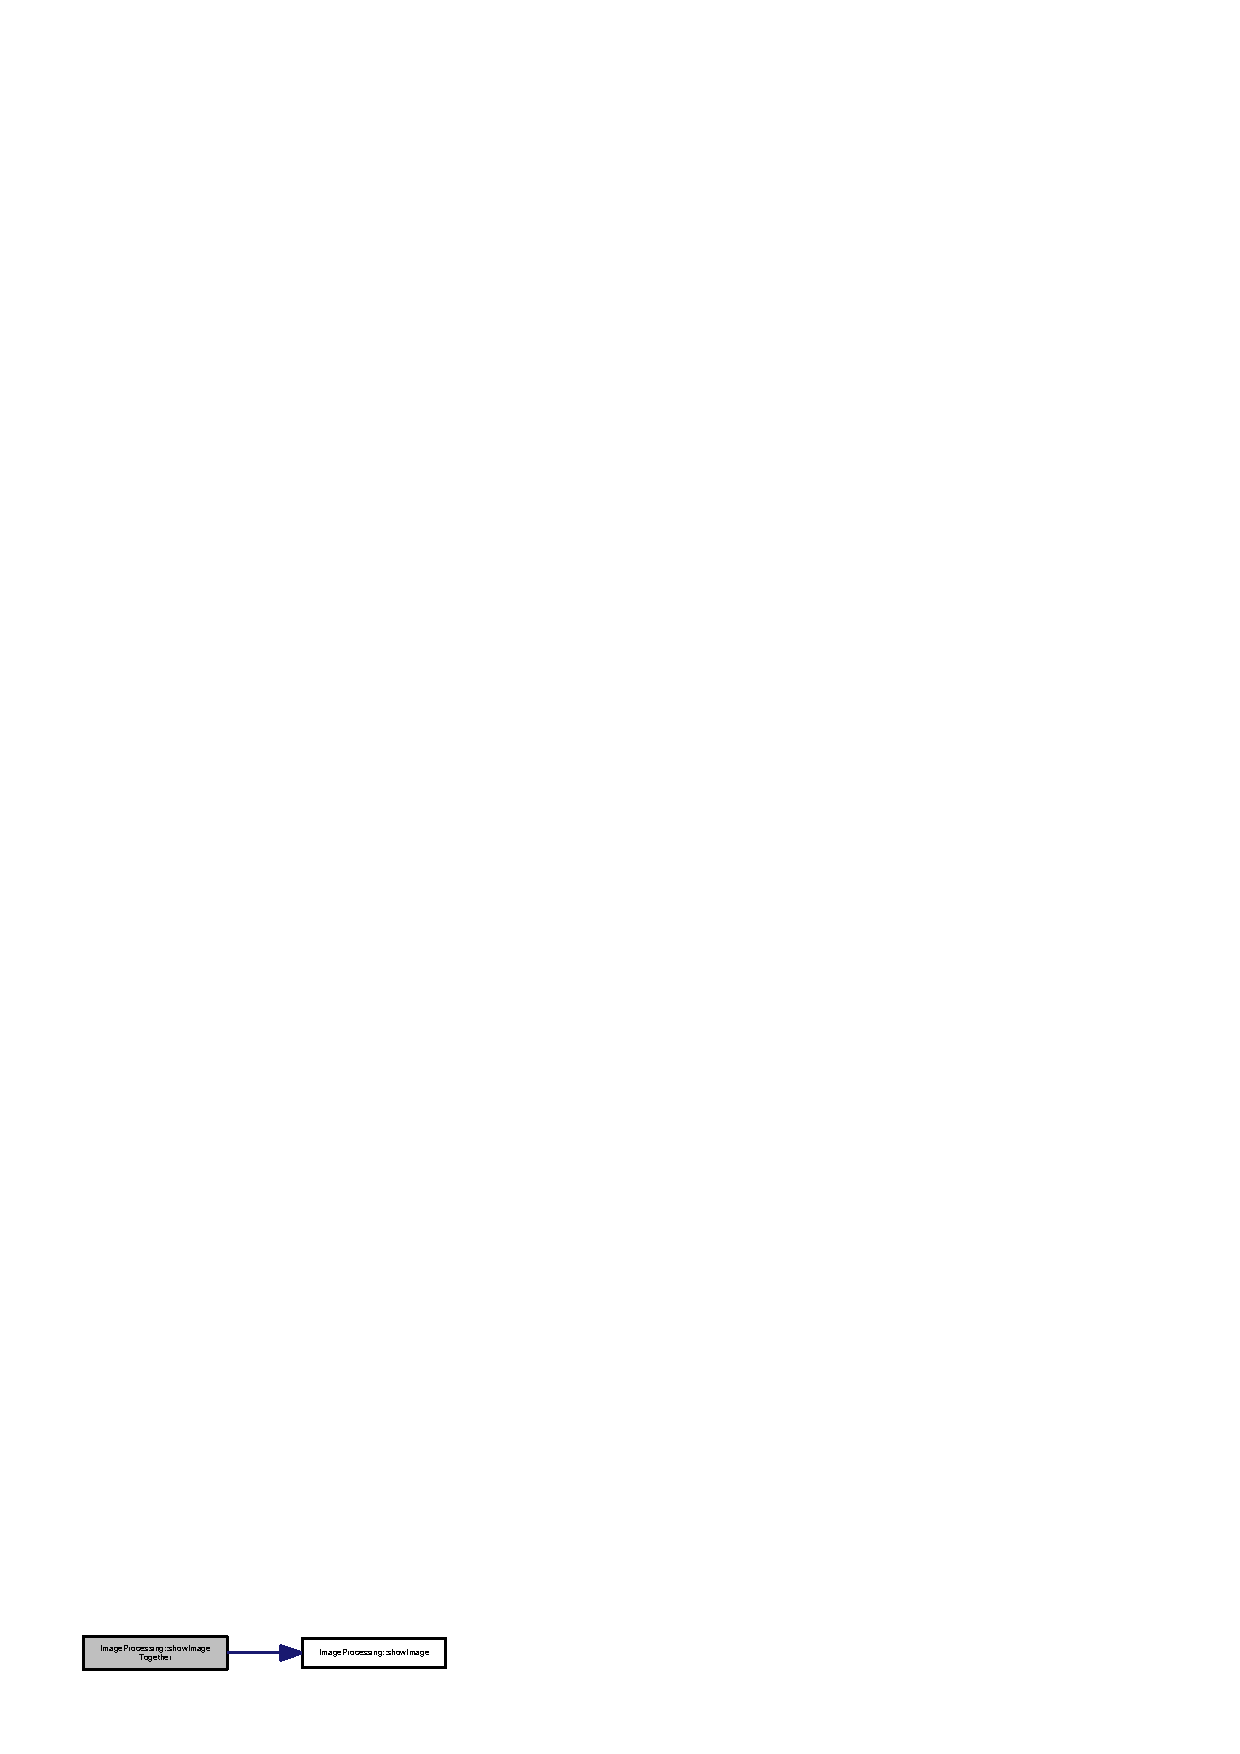
\includegraphics[width=218pt]{class_image_processing_a6651b85571d04f5f05d530a0c760f562_cgraph}
\end{center}
\end{figure}




\subsection{メンバ詳解}
\index{Image\-Processing@{Image\-Processing}!closing\-\_\-times@{closing\-\_\-times}}
\index{closing\-\_\-times@{closing\-\_\-times}!ImageProcessing@{Image\-Processing}}
\subsubsection[{closing\-\_\-times}]{\setlength{\rightskip}{0pt plus 5cm}int Image\-Processing\-::closing\-\_\-times}\label{class_image_processing_ab2722ccf525edb1d42a45b7f6f530051}


クロージングを行う回数 



 Image\-Processing.\-hpp の 42 行目に定義があります。



参照元 get\-Background\-Substraction\-Bin\-Image(), Image\-Processing(), open\-C\-V\-Setting\-Trackbar().

\index{Image\-Processing@{Image\-Processing}!neighborhood@{neighborhood}}
\index{neighborhood@{neighborhood}!ImageProcessing@{Image\-Processing}}
\subsubsection[{neighborhood}]{\setlength{\rightskip}{0pt plus 5cm}int Image\-Processing\-::neighborhood}\label{class_image_processing_a4047a0099a07190f555c5c99d311ee42}


平滑化を行うときの近傍 



 Image\-Processing.\-hpp の 41 行目に定義があります。



参照元 get\-Background\-Substraction\-Bin\-Image(), Image\-Processing(), open\-C\-V\-Setting\-Trackbar().

\index{Image\-Processing@{Image\-Processing}!th@{th}}
\index{th@{th}!ImageProcessing@{Image\-Processing}}
\subsubsection[{th}]{\setlength{\rightskip}{0pt plus 5cm}int Image\-Processing\-::th}\label{class_image_processing_a3b07a07726eed8b5e1da00017713068d}


二値化するときの閾値(c82) 



 Image\-Processing.\-hpp の 40 行目に定義があります。



参照元 get\-Background\-Substraction\-Bin\-Image(), Image\-Processing(), open\-C\-V\-Setting\-Trackbar().



このクラス詳解は次のファイルから抽出されました\-:\begin{DoxyCompactItemize}
\item 
{\bf Image\-Processing.\-hpp}\item 
{\bf Image\-Processing.\-cpp}\end{DoxyCompactItemize}

\section{Kinect クラス}
\label{class_kinect}\index{Kinect@{Kinect}}


Kinect操作用のクラス  




{\ttfamily \#include $<$Kinect.\-hpp$>$}

\subsection*{公開メンバ関数}
\begin{DoxyCompactItemize}
\item 
{\bf Kinect} ()
\begin{DoxyCompactList}\small\item\em コンストラクタ \end{DoxyCompactList}\item 
{\bf $\sim$\-Kinect} ()
\begin{DoxyCompactList}\small\item\em デストラクタ \end{DoxyCompactList}\item 
void {\bf initialize} ()
\begin{DoxyCompactList}\small\item\em Kinectの初期化 \end{DoxyCompactList}\item 
void {\bf create\-Instance} ()
\begin{DoxyCompactList}\small\item\em インスタンスの生成 \end{DoxyCompactList}\item 
Mat {\bf draw\-R\-G\-B\-Image} (Mat \&{\bf image})
\begin{DoxyCompactList}\small\item\em R\-G\-Bカメラの処理 \end{DoxyCompactList}\item 
pcl\-::\-Point\-Cloud\\*
$<$ pcl\-::\-Point\-X\-Y\-Z\-R\-G\-B $>$\-::Ptr {\bf get\-Point\-Cloud} (Mat \&Mat\-\_\-image)
\begin{DoxyCompactList}\small\item\em Depthカメラの処理(c57) \end{DoxyCompactList}\item 
int {\bf get\-Distance} (Mat \&{\bf image})
\begin{DoxyCompactList}\small\item\em 距離を取得(c49) \end{DoxyCompactList}\end{DoxyCompactItemize}
\subsection*{公開変数類}
\begin{DoxyCompactItemize}
\item 
H\-A\-N\-D\-L\-E {\bf stream\-Event}
\begin{DoxyCompactList}\small\item\em R\-G\-B,Depthカメラのフレーム更新イベントを待つためのイベントハンドル \end{DoxyCompactList}\item 
int {\bf key}
\begin{DoxyCompactList}\small\item\em ウィンドウ表示のウェイトタイム格納変数 \end{DoxyCompactList}\item 
int {\bf actual\-Extracted\-Num}
\end{DoxyCompactItemize}


\subsection{詳解}
Kinect操作用のクラス 

 Kinect.\-hpp の 31 行目に定義があります。



\subsection{構築子と解体子}
\index{Kinect@{Kinect}!Kinect@{Kinect}}
\index{Kinect@{Kinect}!Kinect@{Kinect}}
\subsubsection[{Kinect}]{\setlength{\rightskip}{0pt plus 5cm}Kinect\-::\-Kinect (
\begin{DoxyParamCaption}
{}
\end{DoxyParamCaption}
)}\label{class_kinect_ab05389f710b912abff1d001edd77d847}


コンストラクタ 

メソッド\-Kinect\-::\-Kinect().コンストラクタ 

 Kinect.\-cpp の 16 行目に定義があります。


\begin{DoxyCode}
17 \{
18     countKinect = 0; \textcolor{comment}{//Kinectの数を初期化}
19 \}
\end{DoxyCode}
\index{Kinect@{Kinect}!$\sim$\-Kinect@{$\sim$\-Kinect}}
\index{$\sim$\-Kinect@{$\sim$\-Kinect}!Kinect@{Kinect}}
\subsubsection[{$\sim$\-Kinect}]{\setlength{\rightskip}{0pt plus 5cm}Kinect\-::$\sim$\-Kinect (
\begin{DoxyParamCaption}
{}
\end{DoxyParamCaption}
)}\label{class_kinect_a3f417dc4deed8106a97f217c26326e12}


デストラクタ 

メソッド\-Kinect\-::$\sim$\-Kinect().デストラクタ 

 Kinect.\-cpp の 24 行目に定義があります。


\begin{DoxyCode}
25 \{
26     \textcolor{comment}{//終了処理}
27     \textcolor{keywordflow}{if} (kinect != 0)\{
28         kinect->NuiShutdown();
29         kinect->Release();
30     \}
31 \}
\end{DoxyCode}


\subsection{関数詳解}
\index{Kinect@{Kinect}!create\-Instance@{create\-Instance}}
\index{create\-Instance@{create\-Instance}!Kinect@{Kinect}}
\subsubsection[{create\-Instance}]{\setlength{\rightskip}{0pt plus 5cm}void Kinect\-::create\-Instance (
\begin{DoxyParamCaption}
{}
\end{DoxyParamCaption}
)}\label{class_kinect_a90ebe68a239488b745a09213f88b4080}


インスタンスの生成 

メソッド\-Kinect\-::create\-Instance().インスタンスの生成 

 Kinect.\-cpp の 36 行目に定義があります。



参照先 E\-R\-R\-O\-R\-\_\-\-C\-H\-E\-C\-K.



参照元 initialize().


\begin{DoxyCode}
37 \{
38     \textcolor{comment}{//接続されているKinectの数を取得する}
39     ERROR_CHECK(::NuiGetSensorCount(&countKinect));
40     \textcolor{keywordflow}{if} (countKinect == 0)\{
41         \textcolor{keywordflow}{throw} runtime\_error(\textcolor{stringliteral}{"Please Connect the Kinect."});
42     \}
43 
44     ERROR_CHECK(::NuiCreateSensorByIndex(0, &kinect)); \textcolor{comment}{//最初のKinectのインスタンスを生成する}
45 
46     \textcolor{comment}{//Kinectの状態を取得する}
47     HRESULT status = kinect->NuiStatus();
48     \textcolor{keywordflow}{if} (status != S\_OK)\{
49         \textcolor{keywordflow}{throw} runtime\_error(\textcolor{stringliteral}{"You Cannot Use the Kinect."});
50 
51     \}
52 
53     \textcolor{keywordflow}{return};
54 \}
\end{DoxyCode}
\index{Kinect@{Kinect}!draw\-R\-G\-B\-Image@{draw\-R\-G\-B\-Image}}
\index{draw\-R\-G\-B\-Image@{draw\-R\-G\-B\-Image}!Kinect@{Kinect}}
\subsubsection[{draw\-R\-G\-B\-Image}]{\setlength{\rightskip}{0pt plus 5cm}Mat Kinect\-::draw\-R\-G\-B\-Image (
\begin{DoxyParamCaption}
\item[{Mat \&}]{image}
\end{DoxyParamCaption}
)}\label{class_kinect_a00f185eb803cc53eb6273000913d9892}


R\-G\-Bカメラの処理 

メソッド\-Kinect\-::draw\-R\-G\-B\-Image(\-Mat\& image).R\-G\-Bカメラの処理


\begin{DoxyParams}{引数}
{\em cv\-::\-Mat\&} & image \\
\hline
\end{DoxyParams}
\begin{DoxyReturn}{戻り値}
cv\-::\-Mat image 
\end{DoxyReturn}


 Kinect.\-cpp の 82 行目に定義があります。



参照先 E\-R\-R\-O\-R\-\_\-\-C\-H\-E\-C\-K.



参照元 main().


\begin{DoxyCode}
83 \{
84     \textcolor{keywordflow}{try}\{
85         \textcolor{comment}{//RGBカメラのフレームデータを取得する}
86         NUI\_IMAGE\_FRAME imageFrame = \{ 0 \};
87         ERROR_CHECK(kinect->NuiImageStreamGetNextFrame(imageStreamHandle, 0, &imageFrame));
88 
89         \textcolor{comment}{//画像データの取得}
90         NUI\_LOCKED\_RECT colorData;
91         imageFrame.pFrameTexture->LockRect(0, &colorData, 0, 0);
92 
93         \textcolor{comment}{//画像データのコピー}
94         image = Mat(height, width, CV\_8UC4, colorData.pBits);
95 
96         \textcolor{comment}{//フレームデータの解放}
97         ERROR_CHECK(kinect->NuiImageStreamReleaseFrame(imageStreamHandle, &imageFrame));
98     \}
99     \textcolor{keywordflow}{catch} (exception& ex)\{ \textcolor{comment}{//例外処理(c57)}
100         cout << ex.what() << endl;
101     \}
102     \textcolor{keywordflow}{return} (image); \textcolor{comment}{//RGBカメラから画像を取得し返す(c30)}
103 \}
\end{DoxyCode}
\index{Kinect@{Kinect}!get\-Distance@{get\-Distance}}
\index{get\-Distance@{get\-Distance}!Kinect@{Kinect}}
\subsubsection[{get\-Distance}]{\setlength{\rightskip}{0pt plus 5cm}int Kinect\-::get\-Distance (
\begin{DoxyParamCaption}
\item[{Mat \&}]{image}
\end{DoxyParamCaption}
)}\label{class_kinect_a9f34af278ca313094fdf472298c3433f}


距離を取得(c49) 

\index{Kinect@{Kinect}!get\-Point\-Cloud@{get\-Point\-Cloud}}
\index{get\-Point\-Cloud@{get\-Point\-Cloud}!Kinect@{Kinect}}
\subsubsection[{get\-Point\-Cloud}]{\setlength{\rightskip}{0pt plus 5cm}pcl\-::\-Point\-Cloud$<$ pcl\-::\-Point\-X\-Y\-Z\-R\-G\-B $>$\-::Ptr Kinect\-::get\-Point\-Cloud (
\begin{DoxyParamCaption}
\item[{Mat \&}]{Mat\-\_\-image}
\end{DoxyParamCaption}
)}\label{class_kinect_a26f88eae66c74699487869d10adb0945}


Depthカメラの処理(c57) 



 Kinect.\-cpp の 110 行目に定義があります。



参照先 C\-A\-M\-E\-R\-A\-\_\-\-R\-E\-S\-O\-L\-U\-T\-I\-O\-N, E\-R\-R\-O\-R\-\_\-\-C\-H\-E\-C\-K, image.



参照元 main().


\begin{DoxyCode}
111 \{
112     \textcolor{keywordflow}{try}\{
113         pcl::PointCloud<pcl::PointXYZRGB>::Ptr points(\textcolor{keyword}{new} pcl::PointCloud<pcl::PointXYZRGB>()); \textcolor{comment}{//
      ポイントクラウド保存用(c57)}
114         points->width = width;
115         points->height = height;
116 
117         \textcolor{comment}{//距離カメラのフレームデータを取得}
118         NUI\_IMAGE\_FRAME depthFrame = \{ 0 \};
119         ERROR_CHECK(kinect->NuiImageStreamGetNextFrame(depthStreamHandle, 0, &depthFrame));
120 
121         \textcolor{comment}{//距離データを取得する}
122         NUI\_LOCKED\_RECT depthData = \{ 0 \};
123         depthFrame.pFrameTexture->LockRect(0, &depthData, 0, 0);
124 
125         USHORT* depth = (USHORT*)depthData.pBits;
126         for (\textcolor{keywordtype}{int} i = 0; i < (depthData.size / \textcolor{keyword}{sizeof}(USHORT)); ++i)\{
127 
128             USHORT distance = ::NuiDepthPixelToDepth(depth[i]);
129 
130             \textcolor{comment}{//USHORT player = ::NuiDepthPixelToPlayerIndex(depth[i]);}
131             LONG depthX = i % width;
132             LONG depthY = i / width;
133             LONG colorX = depthX;
134             LONG colorY = depthY;
135 
136             \textcolor{comment}{// 距離カメラの座標を、RGBカメラの座標に変換する}
137             kinect->NuiImageGetColorPixelCoordinatesFromDepthPixelAtResolution(
      CAMERA_RESOLUTION, CAMERA_RESOLUTION, 0, depthX, depthY, 0\textcolor{comment}{/*depth[i]*/}, &colorX, &colorY);
138 
139             \textcolor{comment}{//点群取得処理.渡された差分画像に応じて条件を入れ替える}
140             \textcolor{comment}{//Vector4 real = NuiTransformDepthImageToSkeleton(depthX, depthY, distance, CAMERA\_RESOLUTION);}
141             Vector4 real = NuiTransformDepthImageToSkeleton(depthX, depthY, distance << 3, 
      CAMERA_RESOLUTION); \textcolor{comment}{//左に3ビットすることでプレーヤー情報を含む深度データを渡し,座標を変換する}
142             \textcolor{keywordflow}{if} (Mat\_image.at<UCHAR>(colorY, colorX) == 255)\{ \textcolor{comment}{//二値画像に対して点群を抽出する際はこっち(白色の点群を抽出)(c70)}
143                 pcl::PointXYZRGB point; \textcolor{comment}{//点群用の変数を確保}
144                 point.x = real.x*1000.0f; \textcolor{comment}{//ポイントクラウドのx座標を格納[mm]}
145                 point.y = real.y*1000.0f; \textcolor{comment}{//ポイントクラウドのy座標を格納[mm]}
146                 point.z = real.z*1000.0f; \textcolor{comment}{//ポイントクラウドのz座標を格納[mm]}
147 
148                 \textcolor{comment}{//cout << point << endl;}
149                 \textcolor{comment}{//テクスチャ(その座標の色を格納していく)}
150                 Vec4b color = image.at<Vec4b>(colorY, colorX); \textcolor{comment}{//色格納用の変数}
151                 point.r = color[2]; \textcolor{comment}{//赤要素}
152                 point.g = color[1]; \textcolor{comment}{//緑要素}
153                 point.b = color[0]; \textcolor{comment}{//青要素}
154                 points->push\_back(point); \textcolor{comment}{//点群を出力}
155             \}
156         \}
157         cloud = points; \textcolor{comment}{//点群をコピー}
158         \textcolor{comment}{//フレームデータを開放する(c58)}
159         ERROR_CHECK(kinect->NuiImageStreamReleaseFrame(depthStreamHandle, &depthFrame));
160     \}
161     \textcolor{keywordflow}{catch} (exception& ex)\{
162         cout << ex.what() << endl;
163     \}
164     \textcolor{keywordflow}{return} cloud;
165 \}\end{DoxyCode}
\index{Kinect@{Kinect}!initialize@{initialize}}
\index{initialize@{initialize}!Kinect@{Kinect}}
\subsubsection[{initialize}]{\setlength{\rightskip}{0pt plus 5cm}void Kinect\-::initialize (
\begin{DoxyParamCaption}
{}
\end{DoxyParamCaption}
)}\label{class_kinect_a79f66d96dc810bf09a9d3cfe4f1f2671}


Kinectの初期化 

メソッド\-Kinect\-::initialize().Kinectの初期化 

 Kinect.\-cpp の 59 行目に定義があります。



参照先 C\-A\-M\-E\-R\-A\-\_\-\-R\-E\-S\-O\-L\-U\-T\-I\-O\-N, create\-Instance(), E\-R\-R\-O\-R\-\_\-\-C\-H\-E\-C\-K, stream\-Event.



参照元 main().


\begin{DoxyCode}
60 \{
61     createInstance(); \textcolor{comment}{//createInstance()の処理へ以降}
62 
63     ERROR_CHECK(kinect->NuiInitialize(NUI\_INITIALIZE\_FLAG\_USES\_COLOR | NUI\_INITIALIZE\_FLAG\_USES\_DEPTH)); \textcolor{comment}{//
      Kinectの設定を初期化}
64     ERROR_CHECK(kinect->NuiImageStreamOpen(NUI\_IMAGE\_TYPE\_COLOR, 
      CAMERA_RESOLUTION, 0, 2, 0, &imageStreamHandle)); \textcolor{comment}{//RGBカメラを初期化}
65     ERROR_CHECK(kinect->NuiImageStreamOpen(NUI\_IMAGE\_TYPE\_DEPTH, 
      CAMERA_RESOLUTION, 0, 2, 0, &depthStreamHandle)); \textcolor{comment}{//Depthカメラを初期化}
66     ERROR_CHECK(kinect->NuiImageStreamSetImageFrameFlags(depthStreamHandle, 
      NUI\_IMAGE\_STREAM\_FLAG\_ENABLE\_NEAR\_MODE)); \textcolor{comment}{//Nearモード}
67 
68     \textcolor{comment}{//フレーム更新のイベントハンドルを作成}
69     streamEvent = ::CreateEvent(0, TRUE, FALSE, 0);
70     ERROR_CHECK(kinect->NuiSetFrameEndEvent(streamEvent, 0));
71 
72     ::NuiImageResolutionToSize(CAMERA_RESOLUTION, width, height); \textcolor{comment}{//指定した解像度の画面サイズを取得する}
73 
74     \textcolor{keywordflow}{return};
75 \}
\end{DoxyCode}


\subsection{メンバ詳解}
\index{Kinect@{Kinect}!actual\-Extracted\-Num@{actual\-Extracted\-Num}}
\index{actual\-Extracted\-Num@{actual\-Extracted\-Num}!Kinect@{Kinect}}
\subsubsection[{actual\-Extracted\-Num}]{\setlength{\rightskip}{0pt plus 5cm}int Kinect\-::actual\-Extracted\-Num}\label{class_kinect_a0ca66b49a986c739058afb116f87a257}


 Kinect.\-hpp の 55 行目に定義があります。

\index{Kinect@{Kinect}!key@{key}}
\index{key@{key}!Kinect@{Kinect}}
\subsubsection[{key}]{\setlength{\rightskip}{0pt plus 5cm}int Kinect\-::key}\label{class_kinect_afe9df20df1f2538ac9ce8b61c409095a}


ウィンドウ表示のウェイトタイム格納変数 



 Kinect.\-hpp の 54 行目に定義があります。



参照元 main().

\index{Kinect@{Kinect}!stream\-Event@{stream\-Event}}
\index{stream\-Event@{stream\-Event}!Kinect@{Kinect}}
\subsubsection[{stream\-Event}]{\setlength{\rightskip}{0pt plus 5cm}H\-A\-N\-D\-L\-E Kinect\-::stream\-Event}\label{class_kinect_a975c1de77489cffc0728ae9817e127c2}


R\-G\-B,Depthカメラのフレーム更新イベントを待つためのイベントハンドル 



 Kinect.\-hpp の 53 行目に定義があります。



参照元 initialize(), main().



このクラス詳解は次のファイルから抽出されました\-:\begin{DoxyCompactItemize}
\item 
{\bf Kinect.\-hpp}\item 
{\bf Kinect.\-cpp}\end{DoxyCompactItemize}

\section{Least\-Square\-Method クラス}
\label{class_least_square_method}\index{Least\-Square\-Method@{Least\-Square\-Method}}


最小二乗法を行うクラス  




{\ttfamily \#include $<$Least\-Square\-Method.\-hpp$>$}

\subsection*{公開メンバ関数}
\begin{DoxyCompactItemize}
\item 
{\bf Least\-Square\-Method} ()
\begin{DoxyCompactList}\small\item\em コンストラクタ \end{DoxyCompactList}\item 
{\bf $\sim$\-Least\-Square\-Method} ()
\begin{DoxyCompactList}\small\item\em デストラクタ \end{DoxyCompactList}\item 
Eigen\-::\-Vector3f {\bf get\-Coefficient} (pcl\-::\-Point\-Cloud$<$ pcl\-::\-Point\-X\-Y\-Z\-R\-G\-B $>$\-::Ptr \&input\-Point\-Cloud)
\begin{DoxyCompactList}\small\item\em 最小二乗法によって平面ax+by+c=0の係数[a b c]'を求めるメソッド \end{DoxyCompactList}\item 
{\bf Attitude\-Angle3d} {\bf calc\-Yaw\-Roll\-Pitch} (Eigen\-::\-Vector3f coefficient\-\_\-plane)
\begin{DoxyCompactList}\small\item\em 最小二乗法によって求めた[a b c]'を用いて平面の姿勢を計算する \end{DoxyCompactList}\end{DoxyCompactItemize}


\subsection{詳解}
最小二乗法を行うクラス 

 Least\-Square\-Method.\-hpp の 20 行目に定義があります。



\subsection{構築子と解体子}
\index{Least\-Square\-Method@{Least\-Square\-Method}!Least\-Square\-Method@{Least\-Square\-Method}}
\index{Least\-Square\-Method@{Least\-Square\-Method}!LeastSquareMethod@{Least\-Square\-Method}}
\subsubsection[{Least\-Square\-Method}]{\setlength{\rightskip}{0pt plus 5cm}Least\-Square\-Method\-::\-Least\-Square\-Method (
\begin{DoxyParamCaption}
{}
\end{DoxyParamCaption}
)}\label{class_least_square_method_a15a1de9d76f1b0f476760297e0c98fd1}


コンストラクタ 

メソッド\-Least\-Square\-Method\-::\-Least\-Square\-Method().コンストラクタ 

 Least\-Square\-Method.\-cpp の 16 行目に定義があります。


\begin{DoxyCode}
17 \{
18     \textcolor{comment}{//繧ウ繝ウ繧ケ繝医Λ繧ッ繧ソ}
19 \}
\end{DoxyCode}
\index{Least\-Square\-Method@{Least\-Square\-Method}!$\sim$\-Least\-Square\-Method@{$\sim$\-Least\-Square\-Method}}
\index{$\sim$\-Least\-Square\-Method@{$\sim$\-Least\-Square\-Method}!LeastSquareMethod@{Least\-Square\-Method}}
\subsubsection[{$\sim$\-Least\-Square\-Method}]{\setlength{\rightskip}{0pt plus 5cm}Least\-Square\-Method\-::$\sim$\-Least\-Square\-Method (
\begin{DoxyParamCaption}
{}
\end{DoxyParamCaption}
)}\label{class_least_square_method_a66e80e4ea9baa065f0bdbc9da48fb077}


デストラクタ 

メソッド\-Least\-Square\-Method\-::$\sim$\-Least\-Square\-Method().デストラクタ 

 Least\-Square\-Method.\-cpp の 24 行目に定義があります。


\begin{DoxyCode}
25 \{
26     \textcolor{comment}{//デストラクタ}
27 \}
\end{DoxyCode}


\subsection{関数詳解}
\index{Least\-Square\-Method@{Least\-Square\-Method}!calc\-Yaw\-Roll\-Pitch@{calc\-Yaw\-Roll\-Pitch}}
\index{calc\-Yaw\-Roll\-Pitch@{calc\-Yaw\-Roll\-Pitch}!LeastSquareMethod@{Least\-Square\-Method}}
\subsubsection[{calc\-Yaw\-Roll\-Pitch}]{\setlength{\rightskip}{0pt plus 5cm}{\bf Attitude\-Angle3d} Least\-Square\-Method\-::calc\-Yaw\-Roll\-Pitch (
\begin{DoxyParamCaption}
\item[{Eigen\-::\-Vector3f}]{coefficient\-\_\-plane}
\end{DoxyParamCaption}
)}\label{class_least_square_method_adf062bbbd7b380abc5f24d3a09d39e47}


最小二乗法によって求めた[a b c]'を用いて平面の姿勢を計算する 

メソッド\-Least\-Square\-Method\-::calc\-Yaw\-Roll\-Pitch().最小二乗法によって求めた[a b c]'を用いて平面の姿勢を計算する 

 Least\-Square\-Method.\-cpp の 77 行目に定義があります。



参照先 Attitude\-Angle\-::pitch, Attitude\-Angle\-::roll, Attitude\-Angle\-::yaw.



参照元 main().


\begin{DoxyCode}
78 \{
79     AttitudeAngle3d attitude\_angle\_rad; \textcolor{comment}{//姿勢角(ラジアン)}
80     AttitudeAngle3d attitude\_angle\_deg; \textcolor{comment}{//姿勢角(度)}
81 
82     \textcolor{comment}{//ヨー角の計算}
83     attitude\_angle\_rad.yaw = -atan(coefficient\_plane.x());
84     attitude\_angle\_deg.yaw = attitude\_angle\_rad.yaw / M\_PI * 180.0;
85 
86     \textcolor{comment}{//ロール角の計算}
87     attitude\_angle\_rad.roll = atan2(-coefficient\_plane.x(), coefficient\_plane.y());
88     attitude\_angle\_deg.roll = attitude\_angle\_rad.roll / M\_PI * 180.0;
89 
90     \textcolor{comment}{//ピッチ角の計算}
91     attitude\_angle\_rad.pitch = atan2(1, coefficient\_plane.y());
92     attitude\_angle\_deg.pitch = attitude\_angle\_rad.pitch / M\_PI * 180.0;
93 
94     \textcolor{keywordflow}{return} attitude\_angle\_deg;
95 \}\end{DoxyCode}
\index{Least\-Square\-Method@{Least\-Square\-Method}!get\-Coefficient@{get\-Coefficient}}
\index{get\-Coefficient@{get\-Coefficient}!LeastSquareMethod@{Least\-Square\-Method}}
\subsubsection[{get\-Coefficient}]{\setlength{\rightskip}{0pt plus 5cm}Eigen\-::\-Vector3f Least\-Square\-Method\-::get\-Coefficient (
\begin{DoxyParamCaption}
\item[{pcl\-::\-Point\-Cloud$<$ pcl\-::\-Point\-X\-Y\-Z\-R\-G\-B $>$\-::Ptr \&}]{input\-Point\-Cloud}
\end{DoxyParamCaption}
)}\label{class_least_square_method_a19559c76884063927045732a38fe043b}


最小二乗法によって平面ax+by+c=0の係数[a b c]'を求めるメソッド 

メソッド\-Least\-Square\-Method\-::get\-Coefficient().最小二乗法によって平面ax+by+c=0の係数[a b c]'を求めるメソッド


\begin{DoxyParams}{引数}
{\em pcl\-::\-Point\-Cloud$<$pcl\-::\-Point\-X\-Y\-A\-R\-G\-B$>$\-::\-Ptr} & \&input\-Point\-Cloud \\
\hline
\end{DoxyParams}
\begin{DoxyReturn}{戻り値}
Eigen\-::\-Vector3f coefficient\-\_\-plane 
\end{DoxyReturn}


 Least\-Square\-Method.\-cpp の 34 行目に定義があります。



参照元 main().


\begin{DoxyCode}
35 \{
36     Eigen::Vector3f coefficient\_plane(0.0, 0.0, 0.0);
37     Eigen::Matrix3f m1;
38     m1.Zero();
39     Eigen::Vector3f m2(0.0, 0.0, 0.0);
40 
41     \textcolor{comment}{//3×3行列 S=[Sxx Sxy Sx;Sxy Syy Sy;Sx Sy inputPointCloud->size()]の初期化}
42     \textcolor{keywordtype}{double} Szz = 0, Sxz = 0, Syz = 0, Sz = 0, Sxx = 0, Sxy = 0, Sx = 0, Syy = 0, Sy = 0;
43     \textcolor{comment}{//最小二乗法によって求めたA=[a b c]'の要素の初期化}
44     \textcolor{comment}{//double a = 0, b = 0, c = 0;}
45     \textcolor{comment}{//cout << "input Size => " << inputPointCloud->size() << endl;}
46     \textcolor{keywordflow}{for} (\textcolor{keywordtype}{int} i = 1; i < inputPointCloud->size(); i++)\{ \textcolor{comment}{//それぞれの要素の計算}
47         Szz = Szz + inputPointCloud->points[i].z * inputPointCloud->points[i].z;
48         Sxz = Sxz + inputPointCloud->points[i].x * inputPointCloud->points[i].z;
49         Syz = Syz + inputPointCloud->points[i].y * inputPointCloud->points[i].z;
50         Sz = Sz + inputPointCloud->points[i].z;
51         Sxx = Sxx + inputPointCloud->points[i].x * inputPointCloud->points[i].x;
52         Sxy = Sxy + inputPointCloud->points[i].x * inputPointCloud->points[i].y;
53         Sx = Sx + inputPointCloud->points[i].x;
54         Syy = Syy + inputPointCloud->points[i].y * inputPointCloud->points[i].y;
55         Sy = Sy + inputPointCloud->points[i].y;
56     \}
57 
58     m1 << Sxx, Sxy, Sx,
59         Sxy, Syy, Sy,
60         Sx, Sy, inputPointCloud->size();
61     \textcolor{comment}{//cout << "m1 => \(\backslash\)n" << m1 << endl;}
62     \textcolor{comment}{//cout << "m1\_inverse => \(\backslash\)n" << m1.inverse() << endl;}
63 
64     m2 << Sxz, Syz, Sz;
65     \textcolor{comment}{//cout << "m2 => \(\backslash\)n" << m2 << endl;}
66 
67     coefficient\_plane = m1.inverse() * m2;
68     \textcolor{comment}{//cout << "coefficient\_plane => \(\backslash\)n" << coefficient\_plane << endl;}
69 
70     \textcolor{keywordflow}{return} coefficient\_plane;
71 \}
\end{DoxyCode}


このクラス詳解は次のファイルから抽出されました\-:\begin{DoxyCompactItemize}
\item 
{\bf Least\-Square\-Method.\-hpp}\item 
{\bf Least\-Square\-Method.\-cpp}\end{DoxyCompactItemize}

\section{output\-Data 構造体}
\label{structoutput_data}\index{output\-Data@{output\-Data}}


ファイルに出力するデータ群(c41)  




{\ttfamily \#include $<$Path\-Tracking\-And\-Induction\-Of\-The\-Robot.\-hpp$>$}

\subsection*{公開変数類}
\begin{DoxyCompactItemize}
\item 
double {\bf total\-Time}
\begin{DoxyCompactList}\small\item\em 合計時間 \end{DoxyCompactList}\item 
float {\bf x}
\begin{DoxyCompactList}\small\item\em x座標 \end{DoxyCompactList}\item 
float {\bf y}
\begin{DoxyCompactList}\small\item\em y座標 \end{DoxyCompactList}\item 
float {\bf z}
\begin{DoxyCompactList}\small\item\em z座標 \end{DoxyCompactList}\end{DoxyCompactItemize}


\subsection{詳解}
ファイルに出力するデータ群(c41) 

 Path\-Tracking\-And\-Induction\-Of\-The\-Robot.\-hpp の 28 行目に定義があります。



\subsection{メンバ詳解}
\index{output\-Data@{output\-Data}!total\-Time@{total\-Time}}
\index{total\-Time@{total\-Time}!outputData@{output\-Data}}
\subsubsection[{total\-Time}]{\setlength{\rightskip}{0pt plus 5cm}double output\-Data\-::total\-Time}\label{structoutput_data_a79c4eabc287b3d1783b3d9d3c036a625}


合計時間 



 Path\-Tracking\-And\-Induction\-Of\-The\-Robot.\-hpp の 29 行目に定義があります。

\index{output\-Data@{output\-Data}!x@{x}}
\index{x@{x}!outputData@{output\-Data}}
\subsubsection[{x}]{\setlength{\rightskip}{0pt plus 5cm}float output\-Data\-::x}\label{structoutput_data_a6bbddab2722a262bf2c3f5b11cfab280}


x座標 



 Path\-Tracking\-And\-Induction\-Of\-The\-Robot.\-hpp の 30 行目に定義があります。

\index{output\-Data@{output\-Data}!y@{y}}
\index{y@{y}!outputData@{output\-Data}}
\subsubsection[{y}]{\setlength{\rightskip}{0pt plus 5cm}float output\-Data\-::y}\label{structoutput_data_a9b56dfa893983cda30d0e082f1a60757}


y座標 



 Path\-Tracking\-And\-Induction\-Of\-The\-Robot.\-hpp の 31 行目に定義があります。

\index{output\-Data@{output\-Data}!z@{z}}
\index{z@{z}!outputData@{output\-Data}}
\subsubsection[{z}]{\setlength{\rightskip}{0pt plus 5cm}float output\-Data\-::z}\label{structoutput_data_abca4e28577dd94f230bcff94199905e8}


z座標 



 Path\-Tracking\-And\-Induction\-Of\-The\-Robot.\-hpp の 32 行目に定義があります。



この構造体詳解は次のファイルから抽出されました\-:\begin{DoxyCompactItemize}
\item 
{\bf Path\-Tracking\-And\-Induction\-Of\-The\-Robot.\-hpp}\end{DoxyCompactItemize}

\section{Point3 構造体}
\label{struct_point3}\index{Point3@{Point3}}


抽出された座標を保存する構造体(c37)  




{\ttfamily \#include $<$Path\-Tracking\-And\-Induction\-Of\-The\-Robot.\-hpp$>$}

\subsection*{公開変数類}
\begin{DoxyCompactItemize}
\item 
int {\bf x}
\begin{DoxyCompactList}\small\item\em x座標 \end{DoxyCompactList}\item 
int {\bf y}
\begin{DoxyCompactList}\small\item\em y座標 \end{DoxyCompactList}\item 
U\-S\-H\-O\-R\-T {\bf z}
\begin{DoxyCompactList}\small\item\em z座標 \end{DoxyCompactList}\end{DoxyCompactItemize}


\subsection{詳解}
抽出された座標を保存する構造体(c37) 

 Path\-Tracking\-And\-Induction\-Of\-The\-Robot.\-hpp の 18 行目に定義があります。



\subsection{メンバ詳解}
\index{Point3@{Point3}!x@{x}}
\index{x@{x}!Point3@{Point3}}
\subsubsection[{x}]{\setlength{\rightskip}{0pt plus 5cm}int Point3\-::x}\label{struct_point3_a92f702275b1efaf2f94dd1ec4906eddc}


x座標 



 Path\-Tracking\-And\-Induction\-Of\-The\-Robot.\-hpp の 19 行目に定義があります。

\index{Point3@{Point3}!y@{y}}
\index{y@{y}!Point3@{Point3}}
\subsubsection[{y}]{\setlength{\rightskip}{0pt plus 5cm}int Point3\-::y}\label{struct_point3_ab6971f71fa10eb79349cd2fdb88ec3f2}


y座標 



 Path\-Tracking\-And\-Induction\-Of\-The\-Robot.\-hpp の 20 行目に定義があります。

\index{Point3@{Point3}!z@{z}}
\index{z@{z}!Point3@{Point3}}
\subsubsection[{z}]{\setlength{\rightskip}{0pt plus 5cm}U\-S\-H\-O\-R\-T Point3\-::z}\label{struct_point3_a205a0d0ecf33c38941118591a5b5a1e2}


z座標 



 Path\-Tracking\-And\-Induction\-Of\-The\-Robot.\-hpp の 21 行目に定義があります。



この構造体詳解は次のファイルから抽出されました\-:\begin{DoxyCompactItemize}
\item 
{\bf Path\-Tracking\-And\-Induction\-Of\-The\-Robot.\-hpp}\end{DoxyCompactItemize}

\section{Point\-Cloud\-Library クラス}
\label{class_point_cloud_library}\index{Point\-Cloud\-Library@{Point\-Cloud\-Library}}


点群処理を行うクラス  




{\ttfamily \#include $<$Point\-Cloud\-Library.\-hpp$>$}

\subsection*{公開メンバ関数}
\begin{DoxyCompactItemize}
\item 
{\bf Point\-Cloud\-Library} ()
\begin{DoxyCompactList}\small\item\em メソッド\-Point\-Cloud\-Library\-::\-Point\-Cloud\-Library().コンストラクタ \end{DoxyCompactList}\item 
{\bf Point\-Cloud\-Library} (bool passthroughflag, bool downsamplingflag, bool statisticaloutlierremovalflag, bool mlsflag, bool extractplaneflag)
\begin{DoxyCompactList}\small\item\em メソッド\-Point\-Cloud\-Library\-::\-Point\-Cloud\-Library().コンストラクタ(c64) \end{DoxyCompactList}\item 
{\bf $\sim$\-Point\-Cloud\-Library} ()
\begin{DoxyCompactList}\small\item\em メソッド\-Point\-Cloud\-Library\-::$\sim$\-Point\-Cloud\-Library().デストラクタ \end{DoxyCompactList}\item 
void {\bf initialize\-Point\-Cloud\-Viewer} (string cloudviewer\-\_\-name)
\begin{DoxyCompactList}\small\item\em ポイントクラウドビューアーを初期化 \end{DoxyCompactList}\item 
void {\bf initialize\-P\-C\-L\-Visualizer} (string pclvisualizer\-\_\-name)
\item 
void {\bf load\-P\-L\-Y} (char $\ast$ply\-\_\-name)
\begin{DoxyCompactList}\small\item\em メソッド\-Point\-Cloud\-Library\-::load\-P\-L\-Y().plyファイルを読み込む \end{DoxyCompactList}\item 
void {\bf flag\-Checker} ()
\begin{DoxyCompactList}\small\item\em メソッド\-Point\-Cloud\-Library\-::flag\-Checker().P\-C\-L処理に関する処理の有無を判定するフラグ変数を反転させるメソッド(c64) \end{DoxyCompactList}\item 
pcl\-::\-Point\-Cloud\\*
$<$ pcl\-::\-Point\-X\-Y\-Z\-R\-G\-B $>$\-::Ptr {\bf pass\-Through\-Filter} (pcl\-::\-Point\-Cloud$<$ pcl\-::\-Point\-X\-Y\-Z\-R\-G\-B $>$\-::Ptr \&input\-Point\-Cloud, char $\ast$axis, float min, float max)
\begin{DoxyCompactList}\small\item\em パススルーフィルタ.zの値の距離に応じてカット可能 \end{DoxyCompactList}\item 
pcl\-::\-Point\-Cloud\\*
$<$ pcl\-::\-Point\-X\-Y\-Z\-R\-G\-B $>$\-::Ptr {\bf remove\-Outlier} (pcl\-::\-Point\-Cloud$<$ pcl\-::\-Point\-X\-Y\-Z\-R\-G\-B $>$\-::Ptr \&input\-Point\-Cloud)
\begin{DoxyCompactList}\small\item\em メソッド\-Point\-Cloud\-Library\-::remove\-Outlier().外れ値を除去するメソッド(c59) \end{DoxyCompactList}\item 
pcl\-::\-Point\-Cloud\\*
$<$ pcl\-::\-Point\-X\-Y\-Z\-R\-G\-B $>$\-::Ptr {\bf radius\-Outlier\-Removal} (pcl\-::\-Point\-Cloud$<$ pcl\-::\-Point\-X\-Y\-Z\-R\-G\-B $>$\-::Ptr \&input\-Point\-Cloud)
\begin{DoxyCompactList}\small\item\em メソッド\-Point\-Cloud\-Library\-::radius\-Outlier\-Removal().外れ値を除去するメソッド(c60) \end{DoxyCompactList}\item 
pcl\-::\-Point\-Cloud\\*
$<$ pcl\-::\-Point\-X\-Y\-Z\-R\-G\-B $>$\-::Ptr {\bf down\-Sampling\-Using\-Voxel\-Grid\-Filter} (pcl\-::\-Point\-Cloud$<$ pcl\-::\-Point\-X\-Y\-Z\-R\-G\-B $>$\-::Ptr \&input\-Point\-Cloud, float leaf\-Size\-X, float leaf\-Size\-Y, float leaf\-Size\-Z)
\begin{DoxyCompactList}\small\item\em ダウンサンプリングの \end{DoxyCompactList}\item 
pcl\-::\-Point\-Cloud\\*
$<$ pcl\-::\-Point\-X\-Y\-Z\-R\-G\-B $>$\-::Ptr {\bf smoothing\-Using\-Moving\-Least\-Square} (pcl\-::\-Point\-Cloud$<$ pcl\-::\-Point\-X\-Y\-Z\-R\-G\-B $>$\-::Ptr \&input\-Point\-Cloud, bool compute\-\_\-normals, bool polynomial\-\_\-fit, double radius)
\begin{DoxyCompactList}\small\item\em スムージング \end{DoxyCompactList}\item 
pcl\-::\-Point\-Cloud\\*
$<$ pcl\-::\-Point\-X\-Y\-Z\-R\-G\-B $>$\-::Ptr {\bf get\-Extract\-Plane\-And\-Clustering} (pcl\-::\-Point\-Cloud$<$ pcl\-::\-Point\-X\-Y\-Z\-R\-G\-B $>$\-::Ptr \&input\-Point\-Cloud, bool optimize, int max\-Iterations, double threshold, bool negative1, bool negative2, double tolerance, int min\-Cluster\-Size, int max\-Cluster\-Size)
\begin{DoxyCompactList}\small\item\em 平面検出とクラスタリング \end{DoxyCompactList}\item 
Point3d {\bf get\-Centroid\-Coordinate3d} (pcl\-::\-Point\-Cloud$<$ pcl\-::\-Point\-X\-Y\-Z\-R\-G\-B $>$\-::Ptr \&input\-Point\-Cloud)
\begin{DoxyCompactList}\small\item\em メソッドget\-Centroid\-Coordinate \end{DoxyCompactList}\item 
pcl\-::\-Point\-Cloud$<$ pcl\-::\-Normal $>$\-::Ptr {\bf get\-Surface\-Normals} (pcl\-::\-Point\-Cloud$<$ pcl\-::\-Point\-X\-Y\-Z\-R\-G\-B $>$\-::Ptr \&input\-Point\-Cloud)
\begin{DoxyCompactList}\small\item\em 法線を計算する \end{DoxyCompactList}\end{DoxyCompactItemize}
\subsection*{公開変数類}
\begin{DoxyCompactItemize}
\item 
pcl\-::\-Point\-Cloud\\*
$<$ pcl\-::\-Point\-X\-Y\-Z\-R\-G\-B $>$\-::Ptr {\bf model}
\item 
Point3d {\bf centroid}
\begin{DoxyCompactList}\small\item\em 平均座標 \end{DoxyCompactList}\item 
pcl\-::visualization\-::\-Cloud\-Viewer $\ast$ {\bf viewer}
\item 
pcl\-::visualization\-::\-P\-C\-L\-Visualizer $\ast$ {\bf visualizer}
\item 
bool {\bf passthrough\-\_\-flag}
\item 
bool {\bf downsampling\-\_\-flag}
\item 
bool {\bf statisticaloutlierremoval\-\_\-flag}
\item 
bool {\bf mls\-\_\-flag}
\item 
bool {\bf extractplane\-\_\-flag}
\end{DoxyCompactItemize}


\subsection{詳解}
点群処理を行うクラス 

 Point\-Cloud\-Library.\-hpp の 20 行目に定義があります。



\subsection{構築子と解体子}
\index{Point\-Cloud\-Library@{Point\-Cloud\-Library}!Point\-Cloud\-Library@{Point\-Cloud\-Library}}
\index{Point\-Cloud\-Library@{Point\-Cloud\-Library}!PointCloudLibrary@{Point\-Cloud\-Library}}
\subsubsection[{Point\-Cloud\-Library}]{\setlength{\rightskip}{0pt plus 5cm}Point\-Cloud\-Library\-::\-Point\-Cloud\-Library (
\begin{DoxyParamCaption}
{}
\end{DoxyParamCaption}
)}\label{class_point_cloud_library_afade3ec02d4cdcf848e2ab972292f0c4}


メソッド\-Point\-Cloud\-Library\-::\-Point\-Cloud\-Library().コンストラクタ 



 Point\-Cloud\-Library.\-cpp の 16 行目に定義があります。


\begin{DoxyCode}
17 \{
18     \textcolor{comment}{//繧ウ繝ウ繧ケ繝医Λ繧ッ繧ソ}
19 \}
\end{DoxyCode}
\index{Point\-Cloud\-Library@{Point\-Cloud\-Library}!Point\-Cloud\-Library@{Point\-Cloud\-Library}}
\index{Point\-Cloud\-Library@{Point\-Cloud\-Library}!PointCloudLibrary@{Point\-Cloud\-Library}}
\subsubsection[{Point\-Cloud\-Library}]{\setlength{\rightskip}{0pt plus 5cm}Point\-Cloud\-Library\-::\-Point\-Cloud\-Library (
\begin{DoxyParamCaption}
\item[{bool}]{passthroughflag, }
\item[{bool}]{downsamplingflag, }
\item[{bool}]{statisticaloutlierremovalflag, }
\item[{bool}]{mlsflag, }
\item[{bool}]{extractplaneflag}
\end{DoxyParamCaption}
)}\label{class_point_cloud_library_ae9975b76a6035d433bcabd076be4c3ee}


メソッド\-Point\-Cloud\-Library\-::\-Point\-Cloud\-Library().コンストラクタ(c64) 


\begin{DoxyParams}{引数}
{\em bool} & flag\-\_\-remove\-Outlier, bool flag\-\_\-downsampling, bool flag\-\_\-\-M\-L\-S, bool flag\-\_\-extract\-Plane \\
\hline
\end{DoxyParams}


 Point\-Cloud\-Library.\-cpp の 25 行目に定義があります。



参照先 downsampling\-\_\-flag, extractplane\-\_\-flag, mls\-\_\-flag, passthrough\-\_\-flag, statisticaloutlierremoval\-\_\-flag.


\begin{DoxyCode}
26 \{
27     \textcolor{comment}{//繧ウ繝ウ繧ケ繝医Λ繧ッ繧ソ}
28     passthrough_flag = passthroughflag;
29     downsampling_flag = downsamplingflag;
30     statisticaloutlierremoval_flag = statisticaloutlierremovalflag;
31     mls_flag = mlsflag;
32     extractplane_flag= extractplaneflag;
33 \}
\end{DoxyCode}
\index{Point\-Cloud\-Library@{Point\-Cloud\-Library}!$\sim$\-Point\-Cloud\-Library@{$\sim$\-Point\-Cloud\-Library}}
\index{$\sim$\-Point\-Cloud\-Library@{$\sim$\-Point\-Cloud\-Library}!PointCloudLibrary@{Point\-Cloud\-Library}}
\subsubsection[{$\sim$\-Point\-Cloud\-Library}]{\setlength{\rightskip}{0pt plus 5cm}Point\-Cloud\-Library\-::$\sim$\-Point\-Cloud\-Library (
\begin{DoxyParamCaption}
{}
\end{DoxyParamCaption}
)}\label{class_point_cloud_library_ab592f569c2ac402971f0b176af8b8c1e}


メソッド\-Point\-Cloud\-Library\-::$\sim$\-Point\-Cloud\-Library().デストラクタ 



 Point\-Cloud\-Library.\-cpp の 38 行目に定義があります。


\begin{DoxyCode}
39 \{
40     \textcolor{comment}{//デストラクタ}
41 \}
\end{DoxyCode}


\subsection{関数詳解}
\index{Point\-Cloud\-Library@{Point\-Cloud\-Library}!down\-Sampling\-Using\-Voxel\-Grid\-Filter@{down\-Sampling\-Using\-Voxel\-Grid\-Filter}}
\index{down\-Sampling\-Using\-Voxel\-Grid\-Filter@{down\-Sampling\-Using\-Voxel\-Grid\-Filter}!PointCloudLibrary@{Point\-Cloud\-Library}}
\subsubsection[{down\-Sampling\-Using\-Voxel\-Grid\-Filter}]{\setlength{\rightskip}{0pt plus 5cm}pcl\-::\-Point\-Cloud$<$ pcl\-::\-Point\-X\-Y\-Z\-R\-G\-B $>$\-::Ptr Point\-Cloud\-Library\-::down\-Sampling\-Using\-Voxel\-Grid\-Filter (
\begin{DoxyParamCaption}
\item[{pcl\-::\-Point\-Cloud$<$ pcl\-::\-Point\-X\-Y\-Z\-R\-G\-B $>$\-::Ptr \&}]{input\-Point\-Cloud, }
\item[{float}]{leaf\-Size\-X, }
\item[{float}]{leaf\-Size\-Y, }
\item[{float}]{leaf\-Size\-Z}
\end{DoxyParamCaption}
)}\label{class_point_cloud_library_abf4a5840ba484d07a775c2c0c9e41a99}


ダウンサンプリングの 

メソッド\-Point\-Cloud\-Library\-::down\-Sampling\-Using\-Voxel\-Grid\-Filter().ダウンサンプリング処理を行うメソッド(c59)


\begin{DoxyParams}{引数}
{\em pcl\-::\-Point\-Cloud$<$pcl\-::\-Point\-X\-Y\-Z$>$\-::\-Ptr} & \&input\-Point\-Cloud \\
\hline
\end{DoxyParams}
\begin{DoxyReturn}{戻り値}
pcl\-::\-Point\-Cloud$<$pcl\-::\-Point\-X\-Y\-Z$>$\-::\-Ptr filtered 
\end{DoxyReturn}


 Point\-Cloud\-Library.\-cpp の 167 行目に定義があります。



参照元 main().


\begin{DoxyCode}
168 \{
169     cout << \textcolor{stringliteral}{"before\(\backslash\)tVoxel Grid Filter\(\backslash\)t=>\(\backslash\)t"} << inputPointCloud->size() << endl;
170 
171     pcl::PointCloud<pcl::PointXYZRGB>::Ptr filtered(\textcolor{keyword}{new} pcl::PointCloud<pcl::PointXYZRGB>()); \textcolor{comment}{//
      フィルタリング後用のポイントクラウドを宣言}
172     pcl::VoxelGrid<pcl::PointXYZRGB> vg;
173 
174     vg.setInputCloud(inputPointCloud);
175     \textcolor{comment}{//sor.setLeafSize()でダウンサンプリングの程度を変更}
176     vg.setLeafSize(leafSizeX, leafSizeY, leafSizeZ);
177     vg.filter(*filtered);
178 
179     \textcolor{comment}{//ポイントクラウドをしっかり保持できているかサイズを確認}
180     cout << \textcolor{stringliteral}{"after\(\backslash\)tVoxel Grid Filter\(\backslash\)t=>\(\backslash\)t"} << filtered->size() << endl; \textcolor{comment}{//出力されるポイントクラウドのサイズ}
181     \textcolor{keywordflow}{return} filtered;
182 \}
\end{DoxyCode}
\index{Point\-Cloud\-Library@{Point\-Cloud\-Library}!flag\-Checker@{flag\-Checker}}
\index{flag\-Checker@{flag\-Checker}!PointCloudLibrary@{Point\-Cloud\-Library}}
\subsubsection[{flag\-Checker}]{\setlength{\rightskip}{0pt plus 5cm}void Point\-Cloud\-Library\-::flag\-Checker (
\begin{DoxyParamCaption}
{}
\end{DoxyParamCaption}
)}\label{class_point_cloud_library_a1ee163b625dc199c44149db55c84bafd}


メソッド\-Point\-Cloud\-Library\-::flag\-Checker().P\-C\-L処理に関する処理の有無を判定するフラグ変数を反転させるメソッド(c64) 



 Point\-Cloud\-Library.\-cpp の 77 行目に定義があります。



参照先 downsampling\-\_\-flag, extractplane\-\_\-flag, mls\-\_\-flag, passthrough\-\_\-flag, statisticaloutlierremoval\-\_\-flag.



参照元 main().


\begin{DoxyCode}
78 \{
79     \textcolor{keywordflow}{if} (GetAsyncKeyState(\textcolor{charliteral}{'X'}))\{ \textcolor{comment}{//Xが入力されたので、パススルーフィルターのフラグを反転}
80         passthrough_flag = !passthrough_flag;
81     \}
82     \textcolor{keywordflow}{if} (GetAsyncKeyState(\textcolor{charliteral}{'C'}))\{ \textcolor{comment}{//Cが入力されたので、ダウンサンプリング処理のフラグを反転}
83         downsampling_flag = !downsampling_flag;
84     \}
85     \textcolor{keywordflow}{if} (GetAsyncKeyState(\textcolor{charliteral}{'V'}))\{ \textcolor{comment}{//Vが入力されたので、統計的な外れ値除去処理のフラグを反転}
86         statisticaloutlierremoval_flag = !statisticaloutlierremoval_flag;
87     \}
88     \textcolor{keywordflow}{if} (GetAsyncKeyState(\textcolor{charliteral}{'B'}))\{  \textcolor{comment}{//Nが入力されたので、MLS処理のフラグを反転}
89         mls_flag = !mls_flag;
90     \}
91     \textcolor{keywordflow}{if} (GetAsyncKeyState(\textcolor{charliteral}{'N'}))\{ \textcolor{comment}{//Mが入力されたので、平面検出のフラグを反転}
92         extractplane_flag = !extractplane_flag;
93     \}
94 
95     cout << \textcolor{stringliteral}{"範囲外除去(X) => "} << passthrough_flag << \textcolor{stringliteral}{" ダウンサンプリング(C) => "} << 
      downsampling_flag << \textcolor{stringliteral}{" 外れ値(V) => "} << statisticaloutlierremoval_flag << \textcolor{stringliteral}{" MLS(B) => "} << 
      mls_flag << \textcolor{stringliteral}{" 平面検出(N) => "} << extractplane_flag << endl;
96     \textcolor{keywordflow}{return};
97 \}
\end{DoxyCode}
\index{Point\-Cloud\-Library@{Point\-Cloud\-Library}!get\-Centroid\-Coordinate3d@{get\-Centroid\-Coordinate3d}}
\index{get\-Centroid\-Coordinate3d@{get\-Centroid\-Coordinate3d}!PointCloudLibrary@{Point\-Cloud\-Library}}
\subsubsection[{get\-Centroid\-Coordinate3d}]{\setlength{\rightskip}{0pt plus 5cm}Point3d Point\-Cloud\-Library\-::get\-Centroid\-Coordinate3d (
\begin{DoxyParamCaption}
\item[{pcl\-::\-Point\-Cloud$<$ pcl\-::\-Point\-X\-Y\-Z\-R\-G\-B $>$\-::Ptr \&}]{input\-Point\-Cloud}
\end{DoxyParamCaption}
)}\label{class_point_cloud_library_ad6ce847f97bd8bc4621a4c6a2c380b78}


メソッドget\-Centroid\-Coordinate 


\begin{DoxyParams}{引数}
{\em pcl\-::\-Point\-Cloud$<$pcl\-::\-Point\-X\-Y\-Z\-R\-G\-B$>$\-::\-Ptr} & \&input\-Point\-Cloud \\
\hline
\end{DoxyParams}
\begin{DoxyReturn}{戻り値}
Point3f centroid 
\end{DoxyReturn}


 Point\-Cloud\-Library.\-cpp の 316 行目に定義があります。



参照元 main().


\begin{DoxyCode}
317 \{
318     \textcolor{comment}{//cout << "inputPointCloud => " << inputPointCloud->size() << endl; //最大のクラスタを受け取れているか確認(c76)}
319     \textcolor{comment}{//FILE *pointcloud; //最終1フレーム分.gnuplotで表示するために点群をファイルに出力する用}
320     \textcolor{comment}{//FILE *centroid; //最終1フレーム分.gnuplotで表示するために平均座標(重心)をファイルに出力する用}
321     Point3d centroid\_coordinate = 0; \textcolor{comment}{//重心座標}
322     Point3d sum\_pointcloud = 0; \textcolor{comment}{//座標の合計}
323 
324     \textcolor{comment}{//char filepath\_pointcloud[NOC];}
325     \textcolor{comment}{//char filepath\_centroid[NOC];}
326     \textcolor{comment}{//sprintf\_s(filepath\_pointcloud, "data/%s/pointcloud.dat", directoryName);}
327     \textcolor{comment}{//sprintf\_s(filepath\_centroid, "data/%s/centroid.dat", directoryName);}
328 
329     \textcolor{comment}{//ファイルオープンgnuplotの確認用}
330     \textcolor{comment}{//fopen\_s(&pointcloud, filepath\_pointcloud, "w"); //}
331     \textcolor{comment}{//fopen\_s(&centroid, filepath\_centroid, "w");}
332 
333     \textcolor{comment}{//summention coordinate. ※inputPointCloud->width == inputPointCloud->size().}
334     \textcolor{keywordflow}{for} (\textcolor{keywordtype}{int} i = 1; i < inputPointCloud->size(); i++)\{
335         \textcolor{comment}{//cout << i << " : " << "[x, y, z] => [ " << inputPointCloud->points[i].x << ", " <<
       inputPointCloud->points[i].y << ", " << inputPointCloud->points[i].z << " ] " << endl;}
336         \textcolor{comment}{//fprintf\_s(pointcloud, "%f %f %f\(\backslash\)n", inputPointCloud->points[i].x, inputPointCloud->points[i].y,
       inputPointCloud->points[i].z); //ファイルに出力}
337         sum\_pointcloud.x = sum\_pointcloud.x + inputPointCloud->points[i].x; \textcolor{comment}{//点群のx座標を足し合わせていく}
338         sum\_pointcloud.y = sum\_pointcloud.y + inputPointCloud->points[i].y; \textcolor{comment}{//点群のy座標を足し合わせていく}
339         sum\_pointcloud.z = sum\_pointcloud.z + inputPointCloud->points[i].z; \textcolor{comment}{//点群のz座標を足し合わせていく}
340         \textcolor{comment}{//cout << i << " : " << "sum\_x => " << sum\_pointcloud.x << ", sum\_y => " << sum\_pointcloud.y << ",
       sum\_z => " << sum\_pointcloud.z << endl;}
341         \textcolor{comment}{//cout << sum\_pointcloud << endl; //確認用}
342     \}
343     \textcolor{comment}{//cout << "SUM => " << sum\_pointcloud << endl; //合計の確認用}
344     centroid\_coordinate.x = sum\_pointcloud.x / inputPointCloud->size(); \textcolor{comment}{//x座標の平均(重心)}
345     centroid\_coordinate.y = sum\_pointcloud.y / inputPointCloud->size(); \textcolor{comment}{//y座標の平均(重心)}
346     centroid\_coordinate.z = sum\_pointcloud.z / inputPointCloud->size(); \textcolor{comment}{//z座標の平均(重心)}
347     \textcolor{comment}{//cout << "Centroid" << centroid\_coordinate << endl; //確認用}
348     
349     \textcolor{comment}{//平均座標(重心)をファイルに出力(確認用)}
350     \textcolor{comment}{//fprintf\_s(centroid, "%f %f %f\(\backslash\)n",centroid\_coordinate.x,centroid\_coordinate.y,centroid\_coordinate.z);}
351 
352     \textcolor{comment}{//ファイルを閉じる(核に尿)}
353     \textcolor{comment}{//fclose(pointcloud);}
354     \textcolor{comment}{//fclose(centroid);}
355 
356     \textcolor{keywordflow}{return} centroid\_coordinate;
357 \}
\end{DoxyCode}
\index{Point\-Cloud\-Library@{Point\-Cloud\-Library}!get\-Extract\-Plane\-And\-Clustering@{get\-Extract\-Plane\-And\-Clustering}}
\index{get\-Extract\-Plane\-And\-Clustering@{get\-Extract\-Plane\-And\-Clustering}!PointCloudLibrary@{Point\-Cloud\-Library}}
\subsubsection[{get\-Extract\-Plane\-And\-Clustering}]{\setlength{\rightskip}{0pt plus 5cm}pcl\-::\-Point\-Cloud$<$ pcl\-::\-Point\-X\-Y\-Z\-R\-G\-B $>$\-::Ptr Point\-Cloud\-Library\-::get\-Extract\-Plane\-And\-Clustering (
\begin{DoxyParamCaption}
\item[{pcl\-::\-Point\-Cloud$<$ pcl\-::\-Point\-X\-Y\-Z\-R\-G\-B $>$\-::Ptr \&}]{input\-Point\-Cloud, }
\item[{bool}]{optimize, }
\item[{int}]{max\-Iterations, }
\item[{double}]{threshold, }
\item[{bool}]{negative1, }
\item[{bool}]{negative2, }
\item[{double}]{tolerance, }
\item[{int}]{min\-Cluster\-Size, }
\item[{int}]{max\-Cluster\-Size}
\end{DoxyParamCaption}
)}\label{class_point_cloud_library_a02bfccb26f68ce7498f0054f7bdd5517}


平面検出とクラスタリング 

メソッド\-Point\-Cloud\-Library\-::extract\-Plane().平面を検出するメソッド


\begin{DoxyParams}{引数}
{\em pcl\-::\-Point\-Cloud$<$pcl\-::\-Point\-X\-Y\-Z$>$\-::\-Ptr} & \&input\-Point\-Cloud \\
\hline
\end{DoxyParams}
\begin{DoxyReturn}{戻り値}
pcl\-::\-Point\-Cloud$<$pcl\-::\-Point\-X\-Y\-Z$>$\-::\-Ptr filtered 
\end{DoxyReturn}


 Point\-Cloud\-Library.\-cpp の 214 行目に定義があります。



参照元 main().


\begin{DoxyCode}
215 \{
216     cout << \textcolor{stringliteral}{"before\(\backslash\)tExtract Plane\(\backslash\)t\(\backslash\)t=>\(\backslash\)t"} << inputPointCloud->size() << endl;
217 
218     pcl::PointCloud<pcl::PointXYZRGB>::Ptr cloud\_plane(\textcolor{keyword}{new} pcl::PointCloud<pcl::PointXYZRGB>());
219     pcl::PointCloud<pcl::PointXYZRGB>::Ptr filtered(\textcolor{keyword}{new} pcl::PointCloud<pcl::PointXYZRGB>());
220     pcl::ModelCoefficients::Ptr coefficients(\textcolor{keyword}{new} pcl::ModelCoefficients);
221     pcl::PointIndices::Ptr inliers(\textcolor{keyword}{new} pcl::PointIndices);
222 
223     \textcolor{comment}{//セグメンテーションオブジェクトの生成}
224     pcl::SACSegmentation<pcl::PointXYZRGB> seg;
225 
226     \textcolor{comment}{//オプション}
227     seg.setOptimizeCoefficients(optimize);
228 
229     \textcolor{comment}{//Mandatory}
230     seg.setModelType(pcl::SACMODEL\_PLANE);
231     seg.setMethodType(pcl::SAC\_RANSAC);
232 
233     \textcolor{comment}{//クラスタリング}
234     seg.setMaxIterations(maxIterations); \textcolor{comment}{//Default->100}
235     \textcolor{comment}{//}
236 
237     seg.setDistanceThreshold(threshold);
238 
239     \textcolor{keywordtype}{int} i = 0, nr\_points = (int)inputPointCloud->points.size();
240     \textcolor{keywordflow}{while} (inputPointCloud->points.size() > 0.3*nr\_points)
241     \{
242         seg.setInputCloud(inputPointCloud);
243         seg.segment(*inliers, *coefficients);
244         \textcolor{keywordflow}{if} (inliers->indices.size() == 0)
245         \{
246             cout << \textcolor{stringliteral}{"Could not estimate a planar model for the given dataset."} << endl;
247             \textcolor{keywordflow}{break};
248         \}
249         pcl::ExtractIndices<pcl::PointXYZRGB> extract;
250         extract.setInputCloud(inputPointCloud);
251         extract.setIndices(inliers);
252         extract.setNegative(negative1); \textcolor{comment}{//true:平面以外を残す.false:平面を残す}
253 
254         extract.filter(*cloud\_plane);
255         \textcolor{comment}{//cout << "PointCloud representing the planar component: " << cloud\_plane->points.size() << endl;
       //平面のサイズ}
256 
257         extract.setNegative(negative2);
258         extract.filter(*filtered);
259         pcl::copyPointCloud(*filtered, *inputPointCloud);
260     \}
261 
262     pcl::search::KdTree<pcl::PointXYZRGB>::Ptr tree(\textcolor{keyword}{new} pcl::search::KdTree<pcl::PointXYZRGB>);
263     tree->setInputCloud(inputPointCloud);
264 
265     std::vector<pcl::PointIndices> cluster\_indices;
266     pcl::EuclideanClusterExtraction<pcl::PointXYZRGB> ec;
267     ec.setClusterTolerance(tolerance); \textcolor{comment}{//単位[m]}
268     ec.setMinClusterSize(minClusterSize); \textcolor{comment}{//最小クラスタの値}
269     ec.setMaxClusterSize(maxClusterSize); \textcolor{comment}{//最大クラスタの値}
270     ec.setSearchMethod(tree); \textcolor{comment}{//検索手法}
271     ec.setInputCloud(inputPointCloud); \textcolor{comment}{//点群を入力}
272     ec.extract(cluster\_indices); \textcolor{comment}{//クラスタ情報を出力}
273 
274     \textcolor{keywordtype}{int} j = 0; \textcolor{comment}{//クラスタのカウント}
275     pcl::PointCloud<pcl::PointXYZRGB>::Ptr cloud\_cluster(\textcolor{keyword}{new} pcl::PointCloud<pcl::PointXYZRGB>); \textcolor{comment}{//
      クラスタに色付後の点群用}
276     pcl::PointCloud<pcl::PointXYZRGB>::Ptr max\_cluster(\textcolor{keyword}{new} pcl::PointCloud<pcl::PointXYZRGB>); \textcolor{comment}{//
      最大のクラスタを探す(c76)}
277     max\_cluster = cloud\_cluster; \textcolor{comment}{//最初のクラスタを最大クラスタとする(c76)}
278 
279     \textcolor{keywordtype}{float} colors[6][3] = \{ \{ 255, 0, 0 \}, \{ 0, 255, 0 \}, \{ 0, 0, 255 \}, \{ 255, 255, 0 \}, \{ 0, 255, 255 \}, \{
       255, 0, 255 \} \}; \textcolor{comment}{//クラスタに色を付ける用}
280     \textcolor{keywordflow}{for} (std::vector<pcl::PointIndices>::const\_iterator it = cluster\_indices.begin(); it != cluster\_indices
      .end(); ++it) \textcolor{comment}{//クラスタを1塊ごとに出力}
281     \{
282         \textcolor{keywordflow}{for} (std::vector<int>::const\_iterator pit = it->indices.begin(); pit != it->indices.end(); ++pit)\{
283             inputPointCloud->points[*pit].r = colors[j % 6][0];
284             inputPointCloud->points[*pit].g = colors[j % 6][1];
285             inputPointCloud->points[*pit].b = colors[j % 6][2];
286             cloud\_cluster->points.push\_back(inputPointCloud->points[*pit]);
287         \}
288 
289         \textcolor{comment}{//最大のクラスタを探す.元のmac\_clusterより新しいクラスタの方が大きければ新しいクラスタをmax\_clusterとする(c76)}
290         \textcolor{keywordflow}{if} (max\_cluster->size() < cloud\_cluster->size())\{
291             pcl::copyPointCloud(*cloud\_cluster, *max\_cluster);
292         \}
293 
294         \textcolor{comment}{//cloud\_cluster->width = cloud\_cluster->points.size();}
295         \textcolor{comment}{//cloud\_cluster->height = 1;}
296         cloud\_cluster->is\_dense = \textcolor{keyword}{true};
297         cout << \textcolor{stringliteral}{"Cluster "} << j << \textcolor{stringliteral}{"\(\backslash\)t\(\backslash\)t\(\backslash\)t=>\(\backslash\)t"} << cloud\_cluster->size() << endl;
298 
299         j++;
300     \}
301 
302     \textcolor{comment}{//cout << "width => " << max\_cluster->width << " height => " << max\_cluster->height << endl;}
303 
304     \textcolor{comment}{//cout << "cloud\_cluster => " << cloud\_cluster->size() << ", max\_cluster => " << max\_cluster->size() <<
       endl;}
305     \textcolor{comment}{//pcl::copyPointCloud(*cloud\_cluster, *filtered); //カラーリングしたクラスタ全てを出力}
306     pcl::copyPointCloud(*max\_cluster, *filtered); \textcolor{comment}{//最大のクラスタのみ出力(c76)}
307     cout << \textcolor{stringliteral}{"after\(\backslash\)tExtract Plane\(\backslash\)t\(\backslash\)t=>\(\backslash\)t"} << filtered->size() << endl;
308     \textcolor{keywordflow}{return} filtered;
309 \}
\end{DoxyCode}
\index{Point\-Cloud\-Library@{Point\-Cloud\-Library}!get\-Surface\-Normals@{get\-Surface\-Normals}}
\index{get\-Surface\-Normals@{get\-Surface\-Normals}!PointCloudLibrary@{Point\-Cloud\-Library}}
\subsubsection[{get\-Surface\-Normals}]{\setlength{\rightskip}{0pt plus 5cm}pcl\-::\-Point\-Cloud$<$ pcl\-::\-Normal $>$\-::Ptr Point\-Cloud\-Library\-::get\-Surface\-Normals (
\begin{DoxyParamCaption}
\item[{pcl\-::\-Point\-Cloud$<$ pcl\-::\-Point\-X\-Y\-Z\-R\-G\-B $>$\-::Ptr \&}]{input\-Point\-Cloud}
\end{DoxyParamCaption}
)}\label{class_point_cloud_library_a08edbe28c7fbc3f0f9b1e857d45ac610}


法線を計算する 

メソッド\-Point\-Cloud\-Library\-::get\-Surface\-Normals().法線を計算する


\begin{DoxyParams}{引数}
{\em pcl\-::\-Point\-Cloud$<$pcl\-::\-Point\-X\-Y\-Z\-R\-G\-B$>$\-::\-Ptr} & \&input\-Point\-Cloud \\
\hline
\end{DoxyParams}
\begin{DoxyReturn}{戻り値}
pcl\-::\-Point\-Cloud$<$pcl\-::\-Normal$>$\-::\-Ptr cloud\-\_\-normals 
\end{DoxyReturn}


 Point\-Cloud\-Library.\-cpp の 364 行目に定義があります。


\begin{DoxyCode}
365 \{
366     pcl::NormalEstimation<pcl::PointXYZRGB, pcl::Normal> ne;
367     ne.setInputCloud(inputPointCloud); \textcolor{comment}{//入力された点群の法線を計算する}
368     pcl::search::KdTree<pcl::PointXYZRGB>::Ptr tree(\textcolor{keyword}{new} pcl::search::KdTree<pcl::PointXYZRGB>());
369     ne.setSearchMethod(tree);
370     pcl::PointCloud<pcl::Normal>::Ptr cloud\_normals(\textcolor{keyword}{new} pcl::PointCloud<pcl::Normal>);
371     ne.setRadiusSearch(0.005);
372     ne.compute(*cloud\_normals);
373 
374     cout << *cloud\_normals << endl;
375     \textcolor{keywordflow}{return} cloud\_normals;
376 \}\end{DoxyCode}
\index{Point\-Cloud\-Library@{Point\-Cloud\-Library}!initialize\-P\-C\-L\-Visualizer@{initialize\-P\-C\-L\-Visualizer}}
\index{initialize\-P\-C\-L\-Visualizer@{initialize\-P\-C\-L\-Visualizer}!PointCloudLibrary@{Point\-Cloud\-Library}}
\subsubsection[{initialize\-P\-C\-L\-Visualizer}]{\setlength{\rightskip}{0pt plus 5cm}void Point\-Cloud\-Library\-::initialize\-P\-C\-L\-Visualizer (
\begin{DoxyParamCaption}
\item[{string}]{pclvisualizer\-\_\-name}
\end{DoxyParamCaption}
)}\label{class_point_cloud_library_a7c0232fc05e878dd58f64c1e6ed8e0b4}


 Point\-Cloud\-Library.\-cpp の 53 行目に定義があります。



参照先 visualizer.



参照元 main().


\begin{DoxyCode}
54 \{
55     visualizer = \textcolor{keyword}{new} pcl::visualization::PCLVisualizer(pclvisualizer\_name); \textcolor{comment}{//PCLVisualizerのウインドウ名}
56     visualizer->setBackgroundColor(0, 0, 0); \textcolor{comment}{//PCLVisualizerの背景色}
57     \textcolor{comment}{//visualizer->setPointCloudRenderingProperties(pcl::visualization::PCL\_VISUALIZER\_POINT\_SIZE, 1, "show
       cloud");}
58     visualizer->addCoordinateSystem(1.0);
59     visualizer->initCameraParameters();
60     \textcolor{keywordflow}{return};
61 \}
\end{DoxyCode}
\index{Point\-Cloud\-Library@{Point\-Cloud\-Library}!initialize\-Point\-Cloud\-Viewer@{initialize\-Point\-Cloud\-Viewer}}
\index{initialize\-Point\-Cloud\-Viewer@{initialize\-Point\-Cloud\-Viewer}!PointCloudLibrary@{Point\-Cloud\-Library}}
\subsubsection[{initialize\-Point\-Cloud\-Viewer}]{\setlength{\rightskip}{0pt plus 5cm}void Point\-Cloud\-Library\-::initialize\-Point\-Cloud\-Viewer (
\begin{DoxyParamCaption}
\item[{string}]{cloudviewer\-\_\-name}
\end{DoxyParamCaption}
)}\label{class_point_cloud_library_a7539694c0625f14897552f4536008757}


ポイントクラウドビューアーを初期化 

メソッド\-Point\-Cloud\-Library\-::initialize\-Point\-Cloud\-Viewer().ポイントクラウドビューアーを初期化するメソッド(c57)


\begin{DoxyParams}{引数}
{\em string} & cloudviewer\-\_\-name \\
\hline
\end{DoxyParams}


 Point\-Cloud\-Library.\-cpp の 47 行目に定義があります。



参照先 viewer.


\begin{DoxyCode}
48 \{
49     viewer = \textcolor{keyword}{new} pcl::visualization::CloudViewer(cloudviewer\_name);
50     \textcolor{keywordflow}{return};
51 \}
\end{DoxyCode}
\index{Point\-Cloud\-Library@{Point\-Cloud\-Library}!load\-P\-L\-Y@{load\-P\-L\-Y}}
\index{load\-P\-L\-Y@{load\-P\-L\-Y}!PointCloudLibrary@{Point\-Cloud\-Library}}
\subsubsection[{load\-P\-L\-Y}]{\setlength{\rightskip}{0pt plus 5cm}void Point\-Cloud\-Library\-::load\-P\-L\-Y (
\begin{DoxyParamCaption}
\item[{char $\ast$}]{ply\-\_\-name}
\end{DoxyParamCaption}
)}\label{class_point_cloud_library_a4cbedddc1feb21c4653d128de7dcd690}


メソッド\-Point\-Cloud\-Library\-::load\-P\-L\-Y().plyファイルを読み込む 


\begin{DoxyParams}{引数}
{\em char$\ast$} & ply\-\_\-name \\
\hline
\end{DoxyParams}


 Point\-Cloud\-Library.\-cpp の 67 行目に定義があります。



参照先 model.


\begin{DoxyCode}
68 \{
69     pcl::io::loadPLYFile(ply\_name, *model); \textcolor{comment}{//plyファイルを読み込みmodelに格納する}
70     cout << \textcolor{stringliteral}{"load "} << ply\_name << \textcolor{stringliteral}{". "} << endl;
71     \textcolor{keywordflow}{return};
72 \}
\end{DoxyCode}
\index{Point\-Cloud\-Library@{Point\-Cloud\-Library}!pass\-Through\-Filter@{pass\-Through\-Filter}}
\index{pass\-Through\-Filter@{pass\-Through\-Filter}!PointCloudLibrary@{Point\-Cloud\-Library}}
\subsubsection[{pass\-Through\-Filter}]{\setlength{\rightskip}{0pt plus 5cm}pcl\-::\-Point\-Cloud$<$ pcl\-::\-Point\-X\-Y\-Z\-R\-G\-B $>$\-::Ptr Point\-Cloud\-Library\-::pass\-Through\-Filter (
\begin{DoxyParamCaption}
\item[{pcl\-::\-Point\-Cloud$<$ pcl\-::\-Point\-X\-Y\-Z\-R\-G\-B $>$\-::Ptr \&}]{input\-Point\-Cloud, }
\item[{char $\ast$}]{axis, }
\item[{float}]{min, }
\item[{float}]{max}
\end{DoxyParamCaption}
)}\label{class_point_cloud_library_a1381846354368f5925e3b4e7d649c902}


パススルーフィルタ.zの値の距離に応じてカット可能 

メソッド\-Point\-Cloud\-Library\-::pass\-Through\-Filter().パススルーフィルタ


\begin{DoxyParams}{引数}
{\em pcl\-::\-Point\-Cloud$<$pcl\-::\-Point\-X\-Y\-Z$>$\-::\-Ptr} & \&input\-Point\-Cloud \\
\hline
\end{DoxyParams}
\begin{DoxyReturn}{戻り値}
pcl\-::\-Point\-Cloud$<$pcl\-::\-Point\-X\-Y\-Z$>$\-::\-Ptr filtered 
\end{DoxyReturn}


 Point\-Cloud\-Library.\-cpp の 103 行目に定義があります。



参照元 main().


\begin{DoxyCode}
104 \{
105     cout << \textcolor{stringliteral}{"before\(\backslash\)tPassThroughFilter\(\backslash\)t=>\(\backslash\)t"} << inputPointCloud->size() << endl;
106 
107     pcl::PointCloud<pcl::PointXYZRGB>::Ptr filtered(\textcolor{keyword}{new} pcl::PointCloud<pcl::PointXYZRGB>()); \textcolor{comment}{//
      フィルター後用のポイントクラウド}
108     pcl::PassThrough<pcl::PointXYZRGB> pass;
109     pass.setInputCloud(inputPointCloud);
110     pass.setFilterFieldName(axis);
111     pass.setFilterLimitsNegative(\textcolor{keyword}{false}); \textcolor{comment}{//setFilterLimits(float min, float max)で指定した範囲以外を削除(c69)}
112     pass.setFilterLimits(min, max);
113     pass.filter(*filtered);
114     
115     cout << \textcolor{stringliteral}{"after\(\backslash\)tPassThroughFilter\(\backslash\)t=>\(\backslash\)t"} << filtered->size() << endl;
116     \textcolor{keywordflow}{return} filtered;
117 \}
\end{DoxyCode}
\index{Point\-Cloud\-Library@{Point\-Cloud\-Library}!radius\-Outlier\-Removal@{radius\-Outlier\-Removal}}
\index{radius\-Outlier\-Removal@{radius\-Outlier\-Removal}!PointCloudLibrary@{Point\-Cloud\-Library}}
\subsubsection[{radius\-Outlier\-Removal}]{\setlength{\rightskip}{0pt plus 5cm}pcl\-::\-Point\-Cloud$<$ pcl\-::\-Point\-X\-Y\-Z\-R\-G\-B $>$\-::Ptr Point\-Cloud\-Library\-::radius\-Outlier\-Removal (
\begin{DoxyParamCaption}
\item[{pcl\-::\-Point\-Cloud$<$ pcl\-::\-Point\-X\-Y\-Z\-R\-G\-B $>$\-::Ptr \&}]{input\-Point\-Cloud}
\end{DoxyParamCaption}
)}\label{class_point_cloud_library_a3731df64289fac15009df853c94bc537}


メソッド\-Point\-Cloud\-Library\-::radius\-Outlier\-Removal().外れ値を除去するメソッド(c60) 


\begin{DoxyParams}{引数}
{\em pcl\-::\-Point\-Cloud$<$pcl\-::\-Point\-X\-Y\-Z$>$\-::\-Ptr} & \&input\-Point\-Cloud \\
\hline
\end{DoxyParams}
\begin{DoxyReturn}{戻り値}
pcl\-::\-Point\-Cloud$<$pcl\-::\-Point\-X\-Y\-Z$>$\-::\-Ptr filtered 
\end{DoxyReturn}


 Point\-Cloud\-Library.\-cpp の 146 行目に定義があります。


\begin{DoxyCode}
147 \{
148     cout << \textcolor{stringliteral}{"before\(\backslash\)tRadiusOutlierRemoval\(\backslash\)t=>\(\backslash\)t"} << inputPointCloud->size() << endl;
149 
150     pcl::PointCloud<pcl::PointXYZRGB>::Ptr filtered(\textcolor{keyword}{new} pcl::PointCloud<pcl::PointXYZRGB>()); \textcolor{comment}{//
      フィルタリング後用のポイントクラウドを宣言}
151     pcl::RadiusOutlierRemoval<pcl::PointXYZRGB> ror;
152 
153     ror.setInputCloud(inputPointCloud);
154     ror.setRadiusSearch(0.8);
155     ror.setMinNeighborsInRadius(2);
156     ror.filter(*filtered);
157 
158     cout << \textcolor{stringliteral}{"after\(\backslash\)tRadiusOutlierRemoval\(\backslash\)t=>\(\backslash\)t"} << filtered->size() << endl;
159     \textcolor{keywordflow}{return} filtered;
160 \}
\end{DoxyCode}
\index{Point\-Cloud\-Library@{Point\-Cloud\-Library}!remove\-Outlier@{remove\-Outlier}}
\index{remove\-Outlier@{remove\-Outlier}!PointCloudLibrary@{Point\-Cloud\-Library}}
\subsubsection[{remove\-Outlier}]{\setlength{\rightskip}{0pt plus 5cm}pcl\-::\-Point\-Cloud$<$ pcl\-::\-Point\-X\-Y\-Z\-R\-G\-B $>$\-::Ptr Point\-Cloud\-Library\-::remove\-Outlier (
\begin{DoxyParamCaption}
\item[{pcl\-::\-Point\-Cloud$<$ pcl\-::\-Point\-X\-Y\-Z\-R\-G\-B $>$\-::Ptr \&}]{input\-Point\-Cloud}
\end{DoxyParamCaption}
)}\label{class_point_cloud_library_a4f27c0dfaae2be0174d733e295d1bf36}


メソッド\-Point\-Cloud\-Library\-::remove\-Outlier().外れ値を除去するメソッド(c59) 


\begin{DoxyParams}{引数}
{\em pcl\-::\-Point\-Cloud$<$pcl\-::\-Point\-X\-Y\-Z$>$\-::\-Ptr} & \&input\-Point\-Cloud \\
\hline
\end{DoxyParams}
\begin{DoxyReturn}{戻り値}
pcl\-::\-Point\-Cloud$<$pcl\-::\-Point\-X\-Y\-Z$>$\-::\-Ptr filtered 
\end{DoxyReturn}


 Point\-Cloud\-Library.\-cpp の 124 行目に定義があります。



参照元 main().


\begin{DoxyCode}
125 \{
126     cout << \textcolor{stringliteral}{"before\(\backslash\)tRemove Outlier\(\backslash\)t\(\backslash\)t=>\(\backslash\)t"} << inputPointCloud->size() << endl;
127 
128     pcl::PointCloud<pcl::PointXYZRGB>::Ptr filtered(\textcolor{keyword}{new} pcl::PointCloud<pcl::PointXYZRGB>()); \textcolor{comment}{//
      フィルタリング後用のポイントクラウドを宣言}
129     pcl::StatisticalOutlierRemoval<pcl::PointXYZRGB> fl;
130     
131     fl.setInputCloud(inputPointCloud);
132     fl.setMeanK(10);
133     fl.setStddevMulThresh(0.1);
134     fl.filter(*filtered);
135     fl.setNegative(\textcolor{keyword}{true});
136 
137     cout << \textcolor{stringliteral}{"after\(\backslash\)tRemove Outlier\(\backslash\)t\(\backslash\)t=>\(\backslash\)t"} << filtered->size() << endl;
138     \textcolor{keywordflow}{return} filtered;
139 \}
\end{DoxyCode}
\index{Point\-Cloud\-Library@{Point\-Cloud\-Library}!smoothing\-Using\-Moving\-Least\-Square@{smoothing\-Using\-Moving\-Least\-Square}}
\index{smoothing\-Using\-Moving\-Least\-Square@{smoothing\-Using\-Moving\-Least\-Square}!PointCloudLibrary@{Point\-Cloud\-Library}}
\subsubsection[{smoothing\-Using\-Moving\-Least\-Square}]{\setlength{\rightskip}{0pt plus 5cm}pcl\-::\-Point\-Cloud$<$ pcl\-::\-Point\-X\-Y\-Z\-R\-G\-B $>$\-::Ptr Point\-Cloud\-Library\-::smoothing\-Using\-Moving\-Least\-Square (
\begin{DoxyParamCaption}
\item[{pcl\-::\-Point\-Cloud$<$ pcl\-::\-Point\-X\-Y\-Z\-R\-G\-B $>$\-::Ptr \&}]{input\-Point\-Cloud, }
\item[{bool}]{compute\-\_\-normals, }
\item[{bool}]{polynomial\-\_\-fit, }
\item[{double}]{radius}
\end{DoxyParamCaption}
)}\label{class_point_cloud_library_a2899ca3f4f6b2f8bce39524fba686e74}


スムージング 

メソッド\-Point\-Cloud\-Library\-::smoothing\-Using\-Moving\-Least\-Square().スムージングを行うメソッド(c60)


\begin{DoxyParams}{引数}
{\em pcl\-::\-Point\-Cloud$<$pcl\-::\-Point\-X\-Y\-Z$>$\-::\-Ptr} & \&input\-Point\-Cloud \\
\hline
\end{DoxyParams}
\begin{DoxyReturn}{戻り値}
pcl\-::\-Point\-Cloud$<$pcl\-::\-Point\-X\-Y\-Z$>$\-::\-Ptr filtered 
\end{DoxyReturn}


 Point\-Cloud\-Library.\-cpp の 189 行目に定義があります。



参照元 main().


\begin{DoxyCode}
190 \{
191     cout << \textcolor{stringliteral}{"before\(\backslash\)tMLS\(\backslash\)t\(\backslash\)t\(\backslash\)t=>\(\backslash\)t"} << inputPointCloud->size() << endl;
192 
193     pcl::PointCloud<pcl::PointXYZRGB>::Ptr filtered(\textcolor{keyword}{new} pcl::PointCloud<pcl::PointXYZRGB>()); \textcolor{comment}{//
      フィルタリング処理後用のポイントクラウド}
194     pcl::search::KdTree<pcl::PointXYZRGB>::Ptr tree(\textcolor{keyword}{new} pcl::search::KdTree<pcl::PointXYZRGB>()); \textcolor{comment}{//
      KdTreeの作成}
195     pcl::MovingLeastSquares<pcl::PointXYZRGB, pcl::PointXYZRGB> mls; \textcolor{comment}{//スムージング処理}
196 
197     mls.setComputeNormals(compute\_normals); \textcolor{comment}{//法線の計算}
198     \textcolor{comment}{//各パラメータの設定}
199     mls.setInputCloud(inputPointCloud);
200     mls.setPolynomialFit(polynomial\_fit);
201     mls.setSearchMethod(tree);
202     mls.setSearchRadius(radius);
203     mls.process(*filtered); \textcolor{comment}{// 出力}
204 
205     cout << \textcolor{stringliteral}{"after\(\backslash\)tMLS\(\backslash\)t\(\backslash\)t\(\backslash\)t=>\(\backslash\)t"} << filtered->size() << endl;
206     \textcolor{keywordflow}{return} filtered;
207 \}
\end{DoxyCode}


\subsection{メンバ詳解}
\index{Point\-Cloud\-Library@{Point\-Cloud\-Library}!centroid@{centroid}}
\index{centroid@{centroid}!PointCloudLibrary@{Point\-Cloud\-Library}}
\subsubsection[{centroid}]{\setlength{\rightskip}{0pt plus 5cm}Point3d Point\-Cloud\-Library\-::centroid}\label{class_point_cloud_library_aa8b11edec4c6910b0a9ad5c5340dcfa2}


平均座標 



 Point\-Cloud\-Library.\-hpp の 44 行目に定義があります。



参照元 main().

\index{Point\-Cloud\-Library@{Point\-Cloud\-Library}!downsampling\-\_\-flag@{downsampling\-\_\-flag}}
\index{downsampling\-\_\-flag@{downsampling\-\_\-flag}!PointCloudLibrary@{Point\-Cloud\-Library}}
\subsubsection[{downsampling\-\_\-flag}]{\setlength{\rightskip}{0pt plus 5cm}bool Point\-Cloud\-Library\-::downsampling\-\_\-flag}\label{class_point_cloud_library_a6bb70f323f325576a505c45edd1f2ebe}


 Point\-Cloud\-Library.\-hpp の 57 行目に定義があります。



参照元 flag\-Checker(), main(), Point\-Cloud\-Library().

\index{Point\-Cloud\-Library@{Point\-Cloud\-Library}!extractplane\-\_\-flag@{extractplane\-\_\-flag}}
\index{extractplane\-\_\-flag@{extractplane\-\_\-flag}!PointCloudLibrary@{Point\-Cloud\-Library}}
\subsubsection[{extractplane\-\_\-flag}]{\setlength{\rightskip}{0pt plus 5cm}bool Point\-Cloud\-Library\-::extractplane\-\_\-flag}\label{class_point_cloud_library_a76c829d2feea3efcb84449a0c360ec43}


 Point\-Cloud\-Library.\-hpp の 60 行目に定義があります。



参照元 flag\-Checker(), main(), Point\-Cloud\-Library().

\index{Point\-Cloud\-Library@{Point\-Cloud\-Library}!mls\-\_\-flag@{mls\-\_\-flag}}
\index{mls\-\_\-flag@{mls\-\_\-flag}!PointCloudLibrary@{Point\-Cloud\-Library}}
\subsubsection[{mls\-\_\-flag}]{\setlength{\rightskip}{0pt plus 5cm}bool Point\-Cloud\-Library\-::mls\-\_\-flag}\label{class_point_cloud_library_a0745fdcbdae44048793a4dce33dfeb4f}


 Point\-Cloud\-Library.\-hpp の 59 行目に定義があります。



参照元 flag\-Checker(), main(), Point\-Cloud\-Library().

\index{Point\-Cloud\-Library@{Point\-Cloud\-Library}!model@{model}}
\index{model@{model}!PointCloudLibrary@{Point\-Cloud\-Library}}
\subsubsection[{model}]{\setlength{\rightskip}{0pt plus 5cm}pcl\-::\-Point\-Cloud$<$pcl\-::\-Point\-X\-Y\-Z\-R\-G\-B$>$\-::Ptr Point\-Cloud\-Library\-::model}\label{class_point_cloud_library_a9353ff5d5de9f4d0cc755c3f6bff8417}


 Point\-Cloud\-Library.\-hpp の 32 行目に定義があります。



参照元 load\-P\-L\-Y().

\index{Point\-Cloud\-Library@{Point\-Cloud\-Library}!passthrough\-\_\-flag@{passthrough\-\_\-flag}}
\index{passthrough\-\_\-flag@{passthrough\-\_\-flag}!PointCloudLibrary@{Point\-Cloud\-Library}}
\subsubsection[{passthrough\-\_\-flag}]{\setlength{\rightskip}{0pt plus 5cm}bool Point\-Cloud\-Library\-::passthrough\-\_\-flag}\label{class_point_cloud_library_a29aa3ebced9106bfc070d557efdbdbcf}


 Point\-Cloud\-Library.\-hpp の 56 行目に定義があります。



参照元 flag\-Checker(), main(), Point\-Cloud\-Library().

\index{Point\-Cloud\-Library@{Point\-Cloud\-Library}!statisticaloutlierremoval\-\_\-flag@{statisticaloutlierremoval\-\_\-flag}}
\index{statisticaloutlierremoval\-\_\-flag@{statisticaloutlierremoval\-\_\-flag}!PointCloudLibrary@{Point\-Cloud\-Library}}
\subsubsection[{statisticaloutlierremoval\-\_\-flag}]{\setlength{\rightskip}{0pt plus 5cm}bool Point\-Cloud\-Library\-::statisticaloutlierremoval\-\_\-flag}\label{class_point_cloud_library_a25f7509ec80771a394266cc98c117a9b}


 Point\-Cloud\-Library.\-hpp の 58 行目に定義があります。



参照元 flag\-Checker(), main(), Point\-Cloud\-Library().

\index{Point\-Cloud\-Library@{Point\-Cloud\-Library}!viewer@{viewer}}
\index{viewer@{viewer}!PointCloudLibrary@{Point\-Cloud\-Library}}
\subsubsection[{viewer}]{\setlength{\rightskip}{0pt plus 5cm}pcl\-::visualization\-::\-Cloud\-Viewer$\ast$ Point\-Cloud\-Library\-::viewer}\label{class_point_cloud_library_a43d9e8806ab9f7e52782604020922339}


 Point\-Cloud\-Library.\-hpp の 50 行目に定義があります。



参照元 initialize\-Point\-Cloud\-Viewer().

\index{Point\-Cloud\-Library@{Point\-Cloud\-Library}!visualizer@{visualizer}}
\index{visualizer@{visualizer}!PointCloudLibrary@{Point\-Cloud\-Library}}
\subsubsection[{visualizer}]{\setlength{\rightskip}{0pt plus 5cm}pcl\-::visualization\-::\-P\-C\-L\-Visualizer$\ast$ Point\-Cloud\-Library\-::visualizer}\label{class_point_cloud_library_a00af6b104220e288f26c2d6f890ccd86}


 Point\-Cloud\-Library.\-hpp の 53 行目に定義があります。



参照元 initialize\-P\-C\-L\-Visualizer(), main().



このクラス詳解は次のファイルから抽出されました\-:\begin{DoxyCompactItemize}
\item 
{\bf Point\-Cloud\-Library.\-hpp}\item 
{\bf Point\-Cloud\-Library.\-cpp}\end{DoxyCompactItemize}

\section{System クラス}
\label{class_system}\index{System@{System}}


システム関連の処理を行うクラス  




{\ttfamily \#include $<$System.\-hpp$>$}

\subsection*{公開メンバ関数}
\begin{DoxyCompactItemize}
\item 
{\bf System} ()
\begin{DoxyCompactList}\small\item\em コンストラクタ \end{DoxyCompactList}\item 
{\bf $\sim$\-System} ()
\begin{DoxyCompactList}\small\item\em デストラクタ \end{DoxyCompactList}\item 
void {\bf countdown\-Timer} (int time\-\_\-sec)
\begin{DoxyCompactList}\small\item\em 引数の時間[sec]に応じてカウントダウンを開始する(c75) \end{DoxyCompactList}\item 
void {\bf start\-Message} ()
\begin{DoxyCompactList}\small\item\em プログラム開始時のメッセージを表示(c26) \end{DoxyCompactList}\item 
void {\bf end\-Message} (int c\-Num)
\begin{DoxyCompactList}\small\item\em プログラム終了時のメッセージを表示(c38) \end{DoxyCompactList}\item 
void {\bf end\-Message} ()
\begin{DoxyCompactList}\small\item\em プログラム終了時のメッセージを表示(c63) \end{DoxyCompactList}\item 
void {\bf show\-Help\-Message} ()
\begin{DoxyCompactList}\small\item\em キー入力に関するヘルプを表示(c86) \end{DoxyCompactList}\item 
void {\bf start\-Timer} ()
\begin{DoxyCompactList}\small\item\em タイマーを開始(c65) \end{DoxyCompactList}\item 
void {\bf end\-Timer} ()
\begin{DoxyCompactList}\small\item\em タイマーを終了(c65) \end{DoxyCompactList}\item 
double {\bf get\-Process\-Timein\-Miliseconds} ()
\begin{DoxyCompactList}\small\item\em 計測した時間をミリ秒単位で取得.\-start\-Timer()とend\-Timer()が実行されていることが前提(c65) \end{DoxyCompactList}\item 
double {\bf get\-Frame\-Rate} ()
\begin{DoxyCompactList}\small\item\em フレームレートを取得.\-start\-Timer()とend\-Timer()が実行されていることが前提(c65) \end{DoxyCompactList}\item 
void {\bf check\-Directory} (const char $\ast$check\-\_\-dirname)
\begin{DoxyCompactList}\small\item\em 引数に与えたファイルやディレクトリが存在するかチェックし,無ければ作成する(c81) \end{DoxyCompactList}\item 
void {\bf make\-Directory\-Based\-Date} ()
\begin{DoxyCompactList}\small\item\em 日付に基づいたディレクトリの作成 \end{DoxyCompactList}\item 
void {\bf make\-Directory} (char $\ast$original\-\_\-path, int create\-\_\-dirnum)
\begin{DoxyCompactList}\small\item\em 指定したディレクトリ以下に新しいディレクトリを作成する( \end{DoxyCompactList}\item 
void {\bf remove\-Directory} ()
\begin{DoxyCompactList}\small\item\em 取得したデータが不要だった場合ディレクトリを削除する \end{DoxyCompactList}\item 
int {\bf alternatives} ()
\begin{DoxyCompactList}\small\item\em 数字の入力をチェックする \end{DoxyCompactList}\item 
void {\bf open\-Directory} ()
\begin{DoxyCompactList}\small\item\em ディレクトリを開く(c38) \end{DoxyCompactList}\item 
Video\-Writer {\bf output\-Video} (const string $\ast$output\-Video\-Name)
\begin{DoxyCompactList}\small\item\em 動画を出力する \end{DoxyCompactList}\end{DoxyCompactItemize}
\subsection*{公開変数類}
\begin{DoxyCompactItemize}
\item 
double {\bf time}
\begin{DoxyCompactList}\small\item\em 処理時間の結果 \end{DoxyCompactList}\item 
double {\bf fps}
\begin{DoxyCompactList}\small\item\em フレームレート \end{DoxyCompactList}\item 
double {\bf sum\-\_\-time}
\begin{DoxyCompactList}\small\item\em 処理の合計時間 \end{DoxyCompactList}\end{DoxyCompactItemize}


\subsection{詳解}
システム関連の処理を行うクラス 

 System.\-hpp の 19 行目に定義があります。



\subsection{構築子と解体子}
\index{System@{System}!System@{System}}
\index{System@{System}!System@{System}}
\subsubsection[{System}]{\setlength{\rightskip}{0pt plus 5cm}System\-::\-System (
\begin{DoxyParamCaption}
{}
\end{DoxyParamCaption}
)}\label{class_system_ae317936c9bcf1374d61745572e0f2f8a}


コンストラクタ 

\doxyref{System\-::\-System()}{p.}{class_system_ae317936c9bcf1374d61745572e0f2f8a}.コンストラクタ 

 System.\-cpp の 15 行目に定義があります。



参照先 fps, sum\-\_\-time, time.

\index{System@{System}!$\sim$\-System@{$\sim$\-System}}
\index{$\sim$\-System@{$\sim$\-System}!System@{System}}
\subsubsection[{$\sim$\-System}]{\setlength{\rightskip}{0pt plus 5cm}System\-::$\sim$\-System (
\begin{DoxyParamCaption}
{}
\end{DoxyParamCaption}
)}\label{class_system_a3be70bb338e3f062f821173fd15680d0}


デストラクタ 

\doxyref{System\-::$\sim$\-System()}{p.}{class_system_a3be70bb338e3f062f821173fd15680d0}.デストラクタ 

 System.\-cpp の 28 行目に定義があります。



\subsection{関数詳解}
\index{System@{System}!alternatives@{alternatives}}
\index{alternatives@{alternatives}!System@{System}}
\subsubsection[{alternatives}]{\setlength{\rightskip}{0pt plus 5cm}int System\-::alternatives (
\begin{DoxyParamCaption}
{}
\end{DoxyParamCaption}
)}\label{class_system_ae6d222fb43f36cb2db3fb7d0bbed1c20}


数字の入力をチェックする 

\doxyref{System\-::alternatives()}{p.}{class_system_ae6d222fb43f36cb2db3fb7d0bbed1c20}.Yes/\-Noの2択のチェック(c21)

\begin{DoxyReturn}{戻り値}
check\-Num int型.\-Yesか\-Noの値 
\end{DoxyReturn}
$<$0か1をチェックするための変数(c27).このメソッドのみで有効な変数(c30) 

 System.\-cpp の 295 行目に定義があります。



参照元 main().



被呼び出し関係図\-:\nopagebreak
\begin{figure}[H]
\begin{center}
\leavevmode
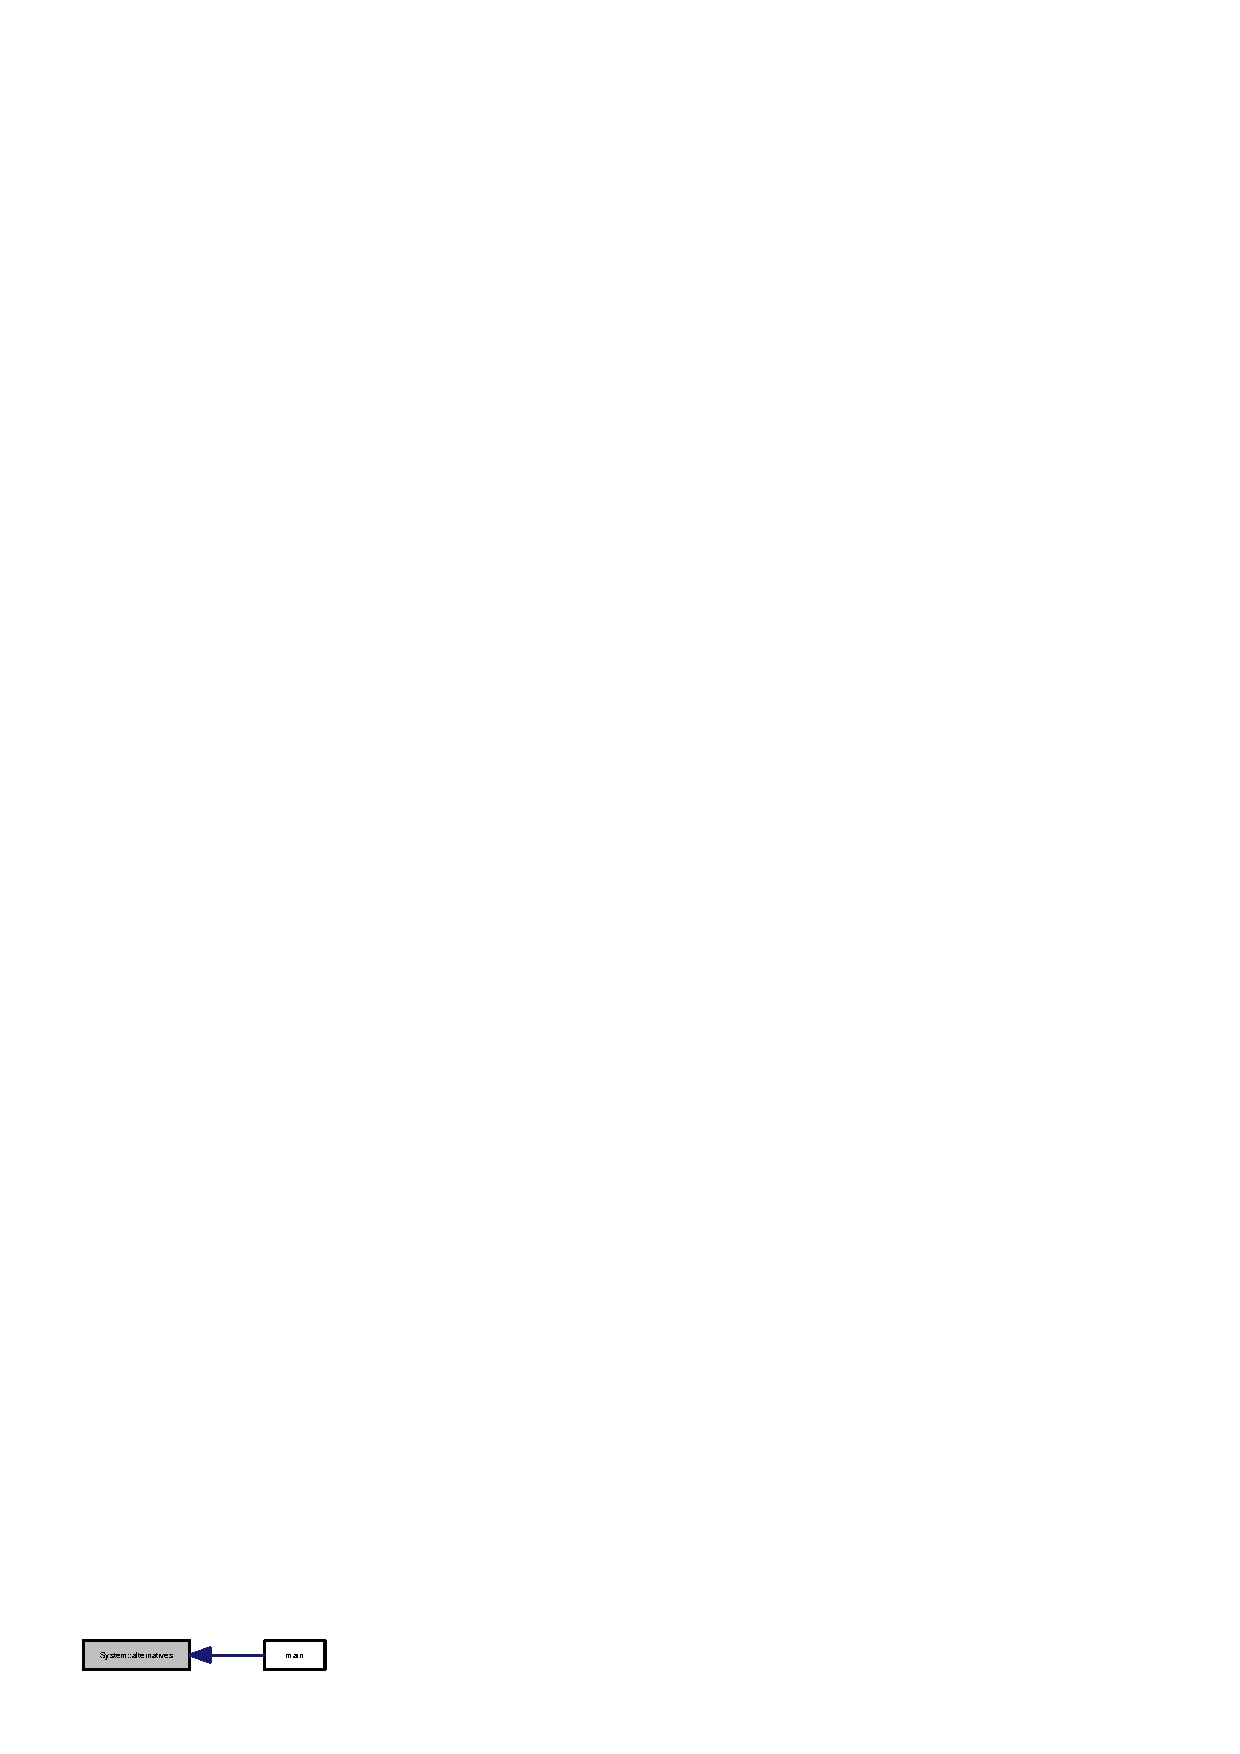
\includegraphics[width=160pt]{class_system_ae6d222fb43f36cb2db3fb7d0bbed1c20_icgraph}
\end{center}
\end{figure}


\index{System@{System}!check\-Directory@{check\-Directory}}
\index{check\-Directory@{check\-Directory}!System@{System}}
\subsubsection[{check\-Directory}]{\setlength{\rightskip}{0pt plus 5cm}void System\-::check\-Directory (
\begin{DoxyParamCaption}
\item[{const char $\ast$}]{check\-\_\-dirname}
\end{DoxyParamCaption}
)}\label{class_system_a2f2eb72dffbb596c530ca149fd8830cd}


引数に与えたファイルやディレクトリが存在するかチェックし,無ければ作成する(c81) 

\doxyref{System\-::check\-Directory()}{p.}{class_system_a2f2eb72dffbb596c530ca149fd8830cd}.ファイルやディレクトリがあるかチェックし,無ければ作成する(c81)


\begin{DoxyParams}{引数}
{\em checkdir\-\_\-name} & const char$\ast$型.ディレクトリ名 \\
\hline
\end{DoxyParams}


 System.\-cpp の 233 行目に定義があります。



参照元 main().



被呼び出し関係図\-:\nopagebreak
\begin{figure}[H]
\begin{center}
\leavevmode
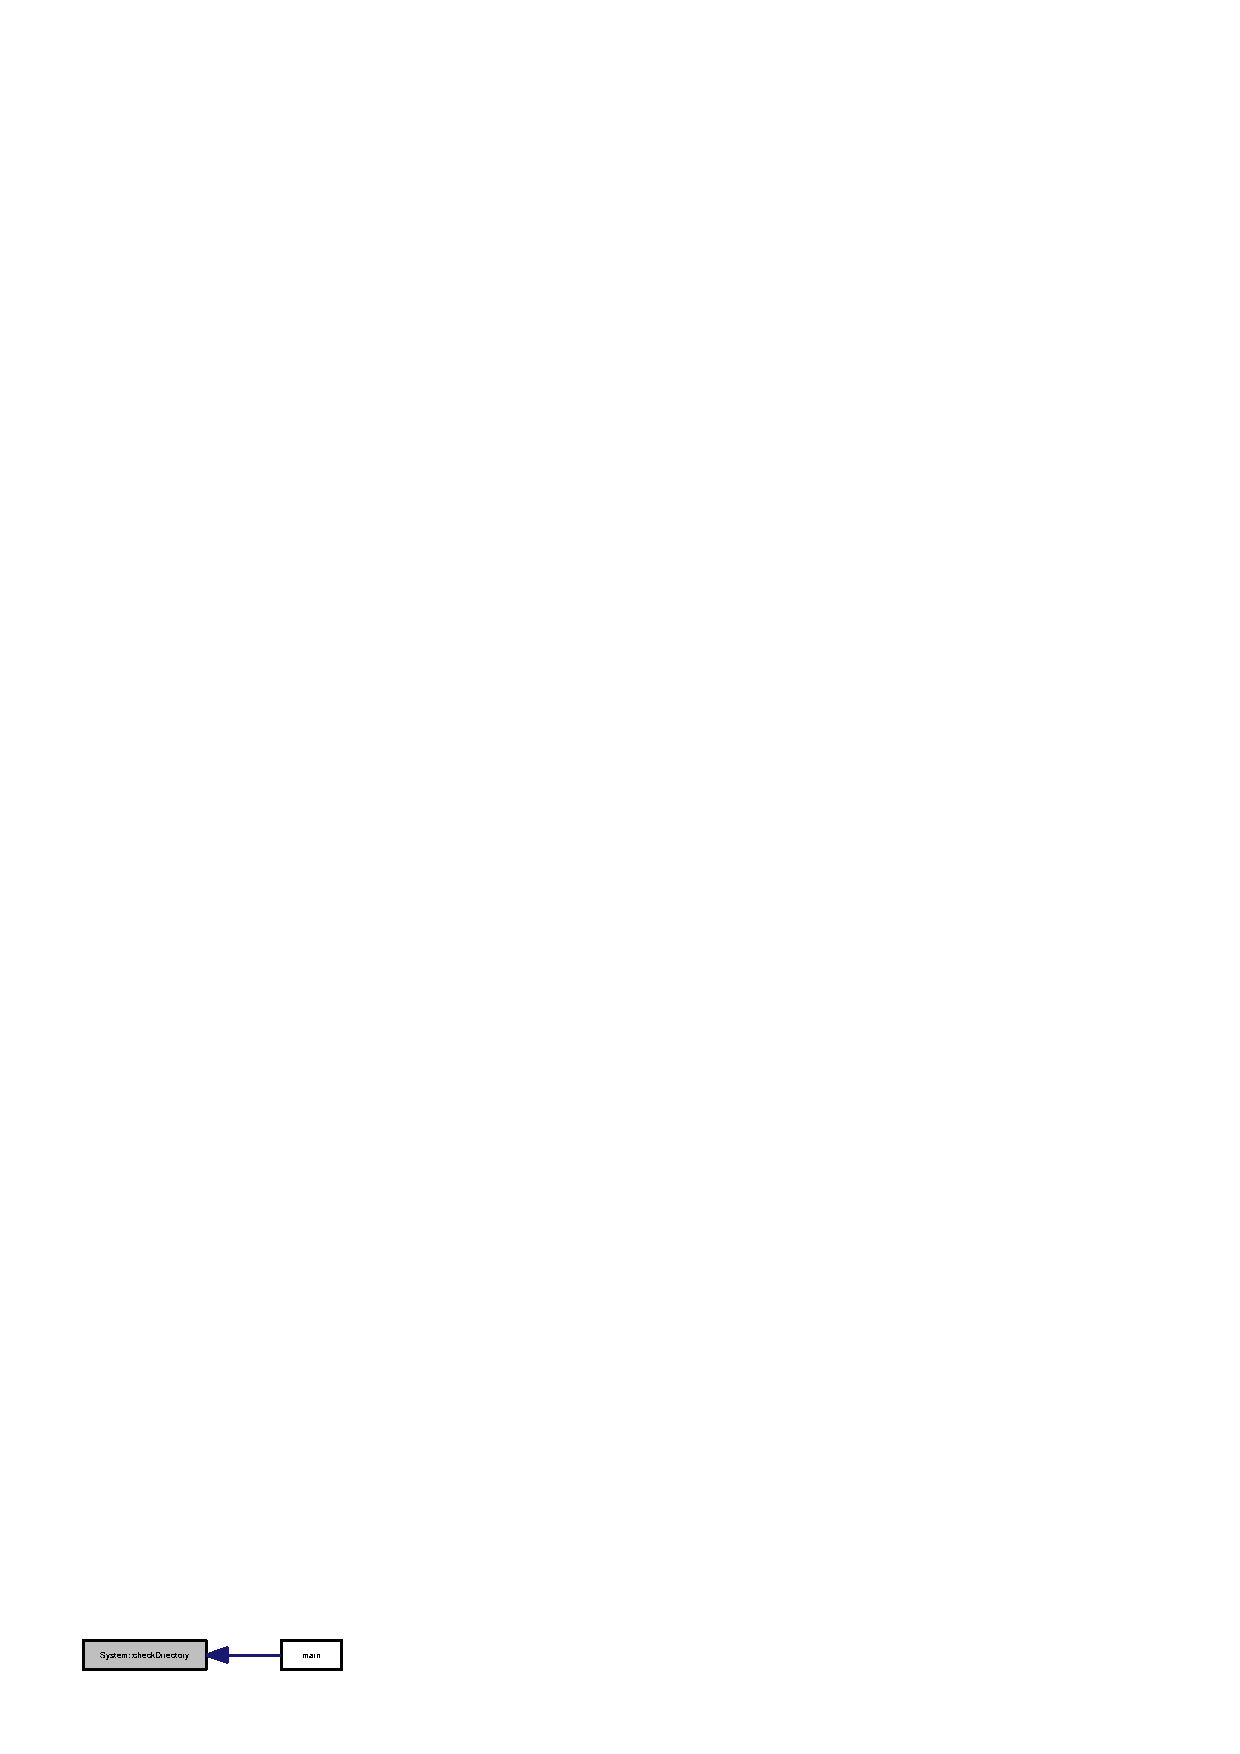
\includegraphics[width=168pt]{class_system_a2f2eb72dffbb596c530ca149fd8830cd_icgraph}
\end{center}
\end{figure}


\index{System@{System}!countdown\-Timer@{countdown\-Timer}}
\index{countdown\-Timer@{countdown\-Timer}!System@{System}}
\subsubsection[{countdown\-Timer}]{\setlength{\rightskip}{0pt plus 5cm}void System\-::countdown\-Timer (
\begin{DoxyParamCaption}
\item[{int}]{time\-\_\-sec}
\end{DoxyParamCaption}
)}\label{class_system_afce9f814824cbcb337abe755883f764c}


引数の時間[sec]に応じてカウントダウンを開始する(c75) 

メソッドcountdown\-Timer().タイマーによるカウントダウン


\begin{DoxyParams}{引数}
{\em time\-\_\-sec} & int型.カウントダウンしたい時間[sec] \\
\hline
\end{DoxyParams}


 System.\-cpp の 108 行目に定義があります。



参照元 main().



被呼び出し関係図\-:\nopagebreak
\begin{figure}[H]
\begin{center}
\leavevmode
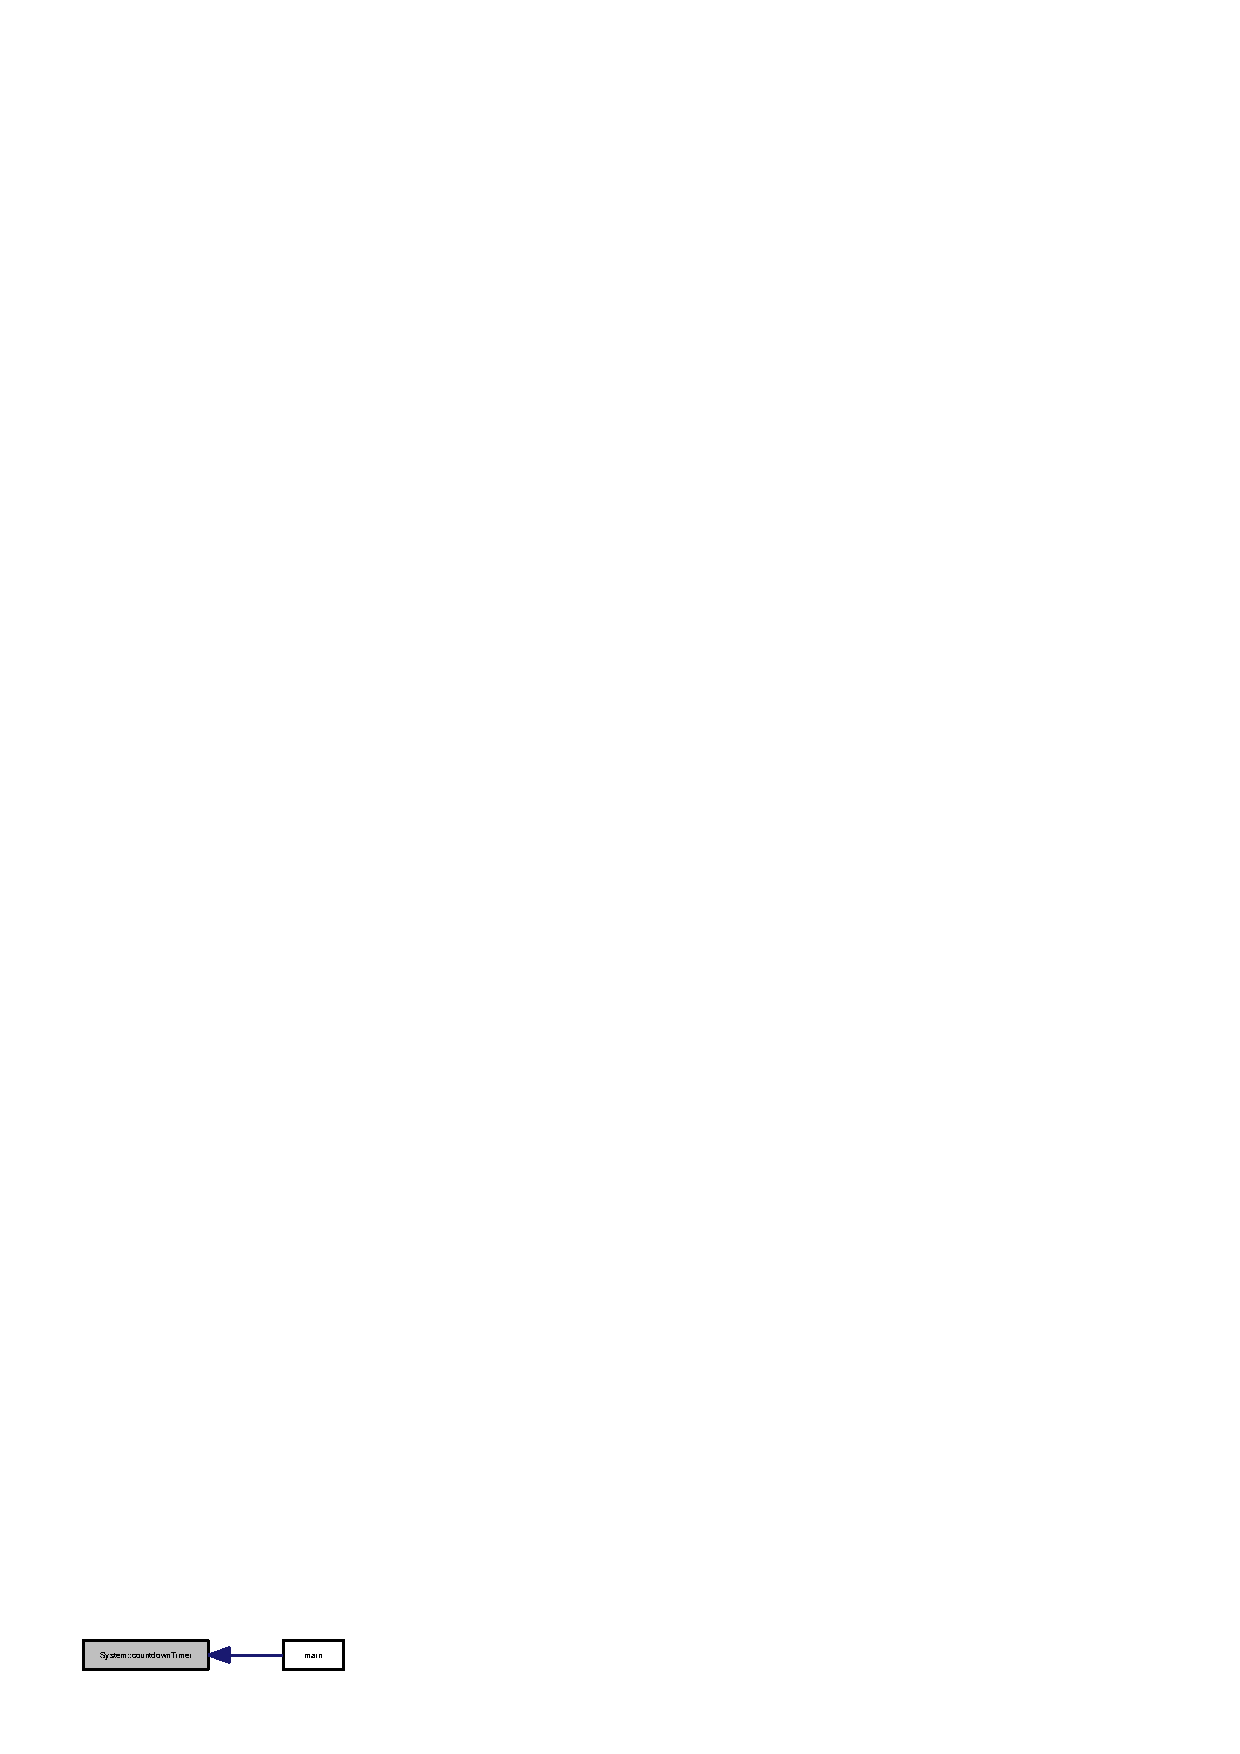
\includegraphics[width=169pt]{class_system_afce9f814824cbcb337abe755883f764c_icgraph}
\end{center}
\end{figure}


\index{System@{System}!end\-Message@{end\-Message}}
\index{end\-Message@{end\-Message}!System@{System}}
\subsubsection[{end\-Message}]{\setlength{\rightskip}{0pt plus 5cm}void System\-::end\-Message (
\begin{DoxyParamCaption}
\item[{int}]{c\-Num}
\end{DoxyParamCaption}
)}\label{class_system_aba9d00b32578f2ea574bf67078db4aa7}


プログラム終了時のメッセージを表示(c38) 

\doxyref{System\-::end\-Message()}{p.}{class_system_a106b76482db29cedc46d4f46b34f3d35}.プログラム終了時のメッセージ 

 System.\-cpp の 60 行目に定義があります。



参照先 directory\-Name, open\-Directory().



参照元 main().



呼び出し関係図\-:\nopagebreak
\begin{figure}[H]
\begin{center}
\leavevmode
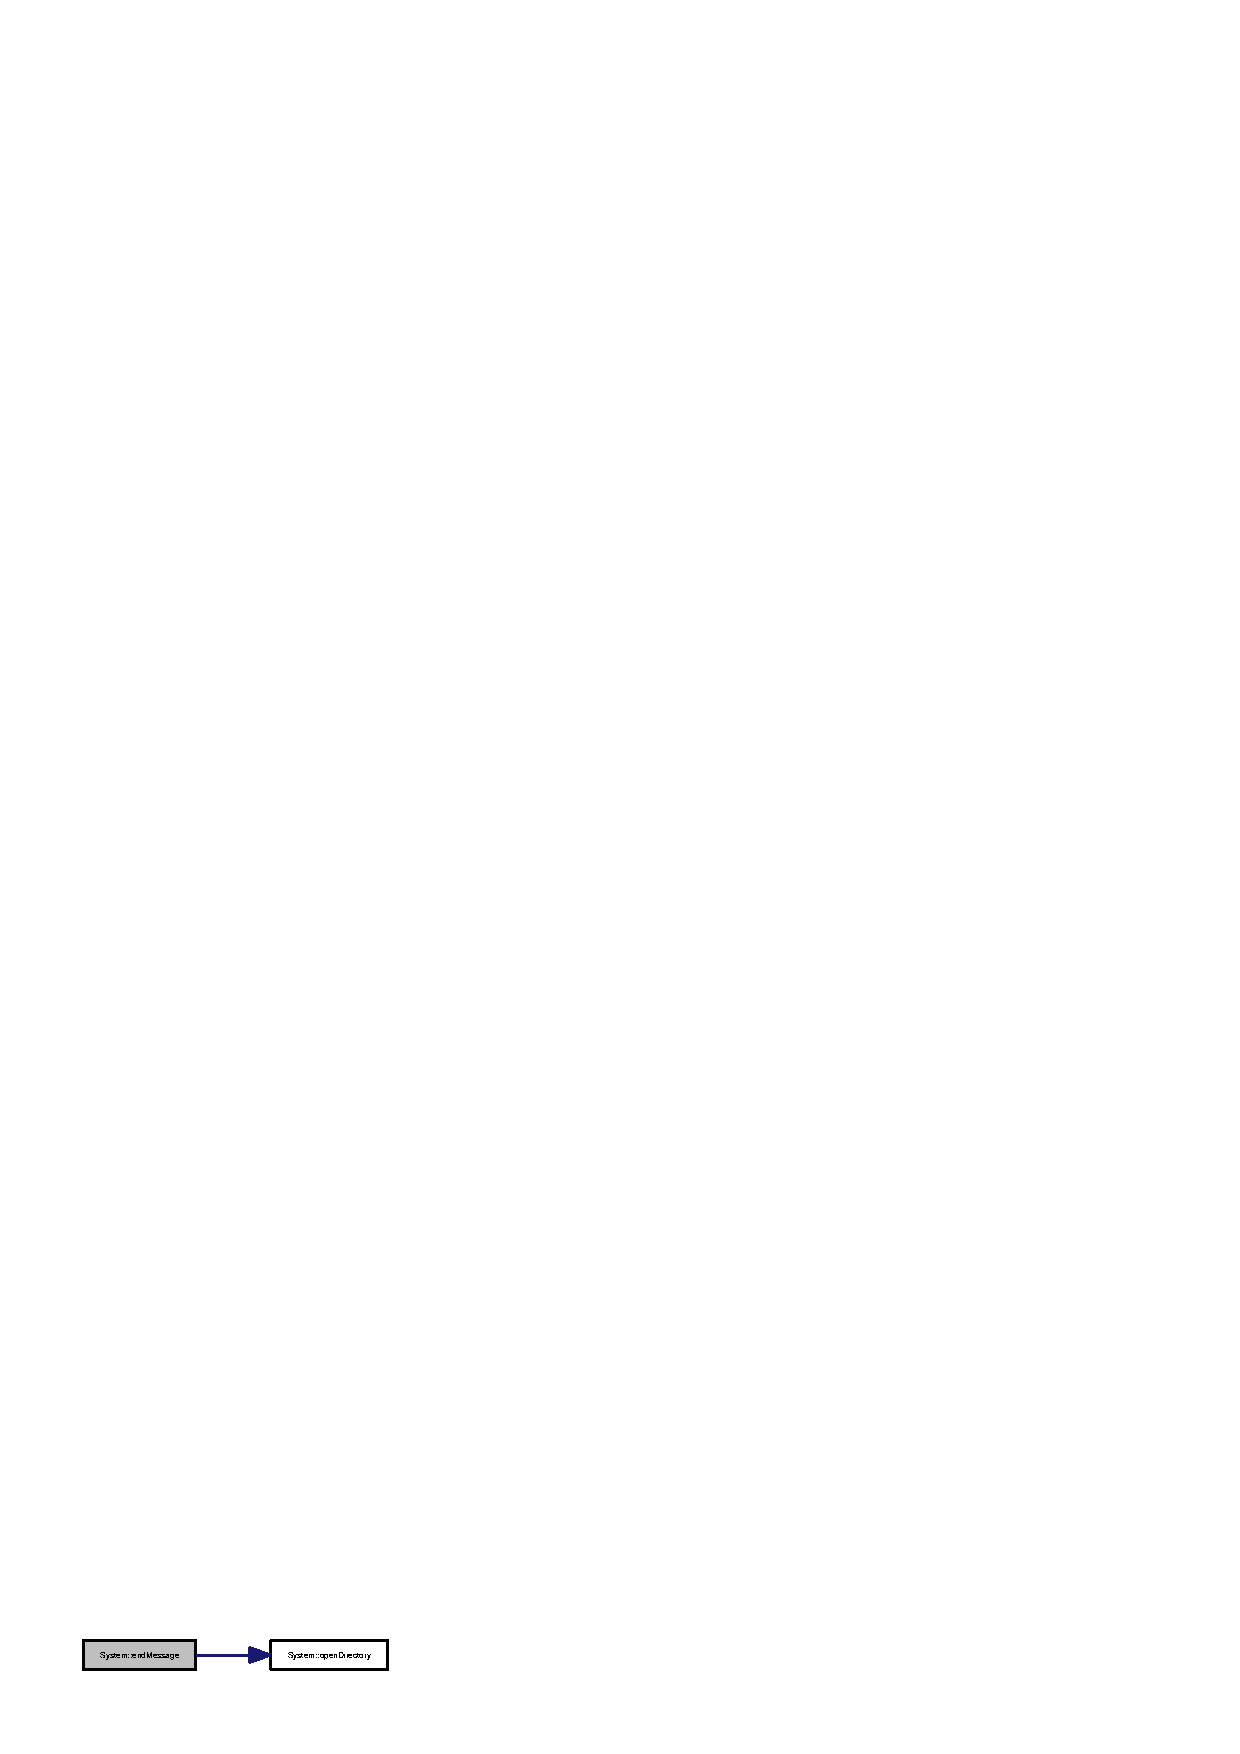
\includegraphics[width=190pt]{class_system_aba9d00b32578f2ea574bf67078db4aa7_cgraph}
\end{center}
\end{figure}




被呼び出し関係図\-:\nopagebreak
\begin{figure}[H]
\begin{center}
\leavevmode
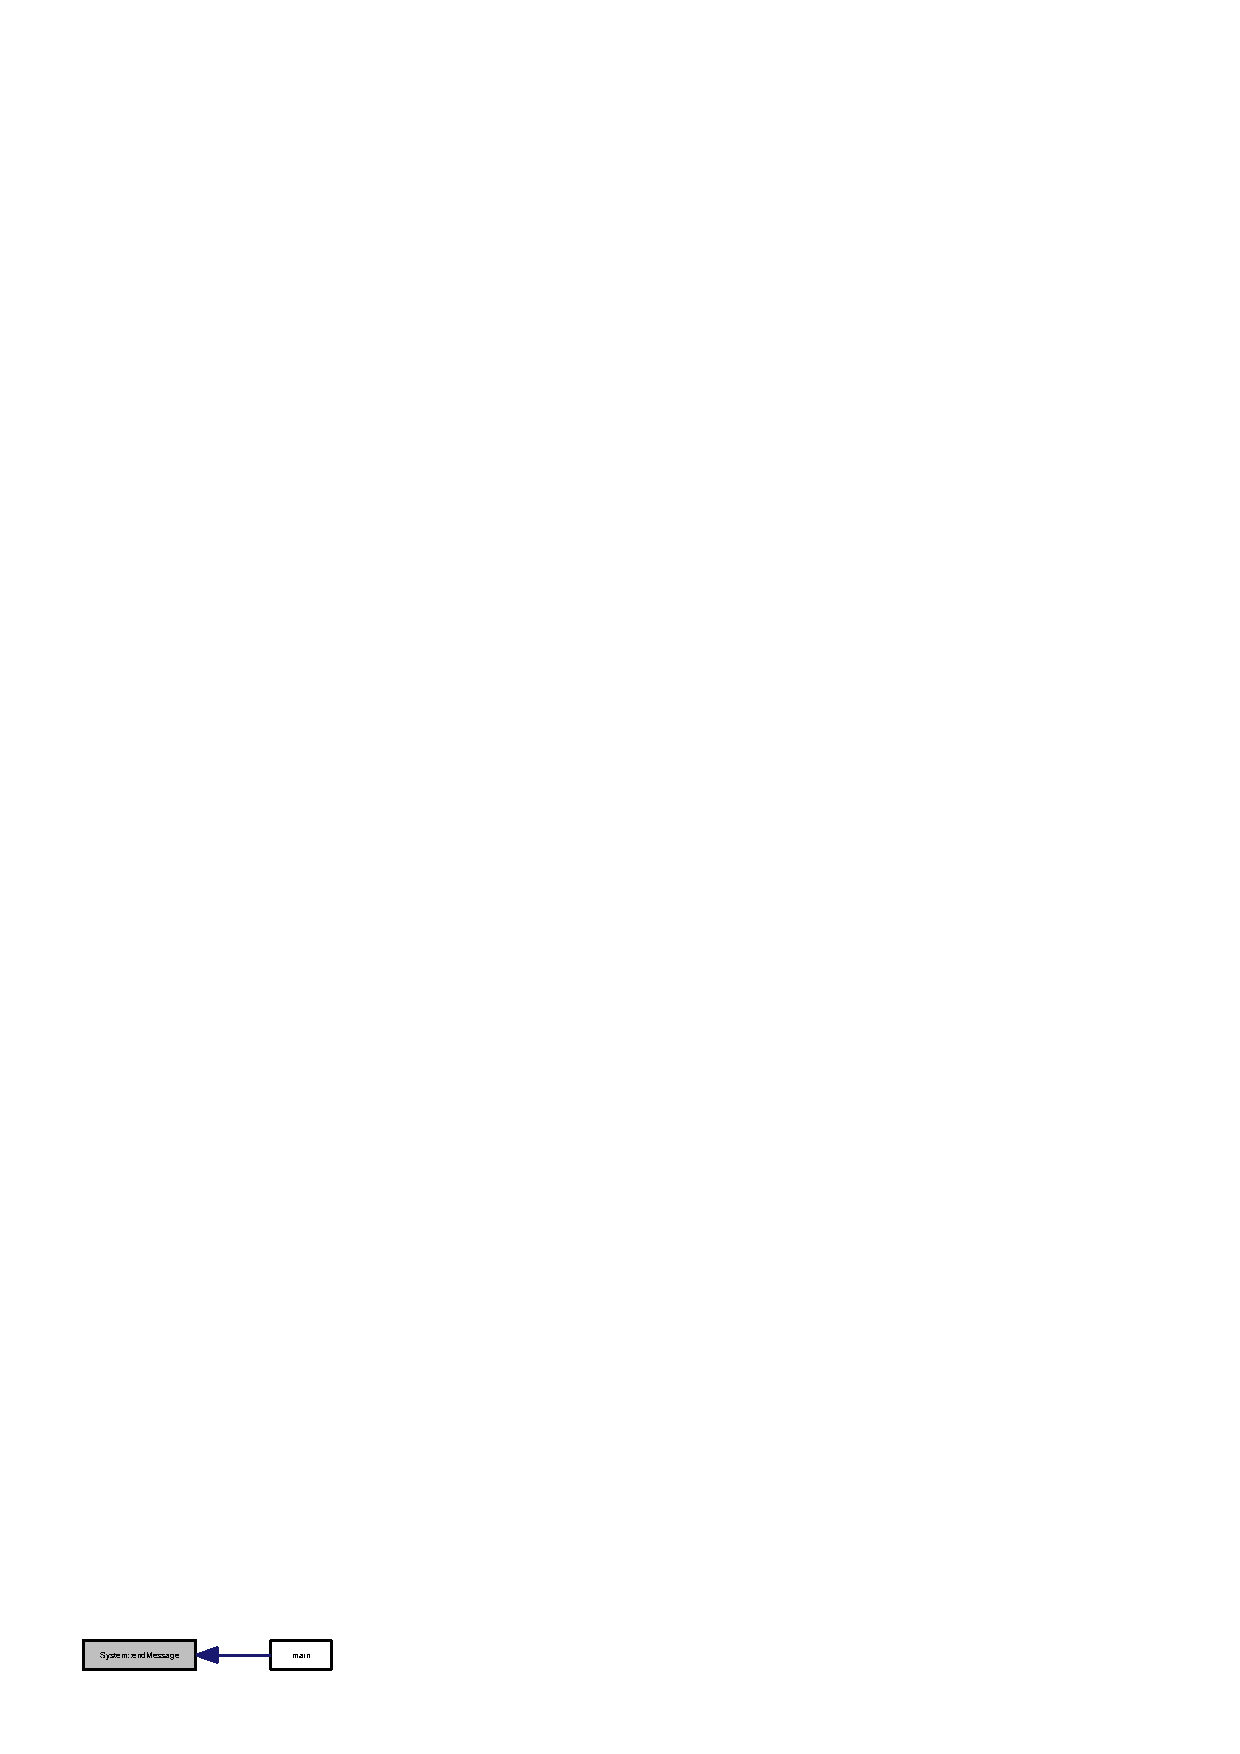
\includegraphics[width=163pt]{class_system_aba9d00b32578f2ea574bf67078db4aa7_icgraph}
\end{center}
\end{figure}


\index{System@{System}!end\-Message@{end\-Message}}
\index{end\-Message@{end\-Message}!System@{System}}
\subsubsection[{end\-Message}]{\setlength{\rightskip}{0pt plus 5cm}void System\-::end\-Message (
\begin{DoxyParamCaption}
{}
\end{DoxyParamCaption}
)}\label{class_system_a106b76482db29cedc46d4f46b34f3d35}


プログラム終了時のメッセージを表示(c63) 

\doxyref{System\-::end\-Message()}{p.}{class_system_a106b76482db29cedc46d4f46b34f3d35}.プログラム終了時のメッセージ 

 System.\-cpp の 76 行目に定義があります。

\index{System@{System}!end\-Timer@{end\-Timer}}
\index{end\-Timer@{end\-Timer}!System@{System}}
\subsubsection[{end\-Timer}]{\setlength{\rightskip}{0pt plus 5cm}void System\-::end\-Timer (
\begin{DoxyParamCaption}
{}
\end{DoxyParamCaption}
)}\label{class_system_a178a7a315866961f208b6cab6c2d7e88}


タイマーを終了(c65) 

メソッドend\-Timer().タイマーを終了する 

 System.\-cpp の 168 行目に定義があります。



参照先 time.



参照元 main().



被呼び出し関係図\-:\nopagebreak
\begin{figure}[H]
\begin{center}
\leavevmode
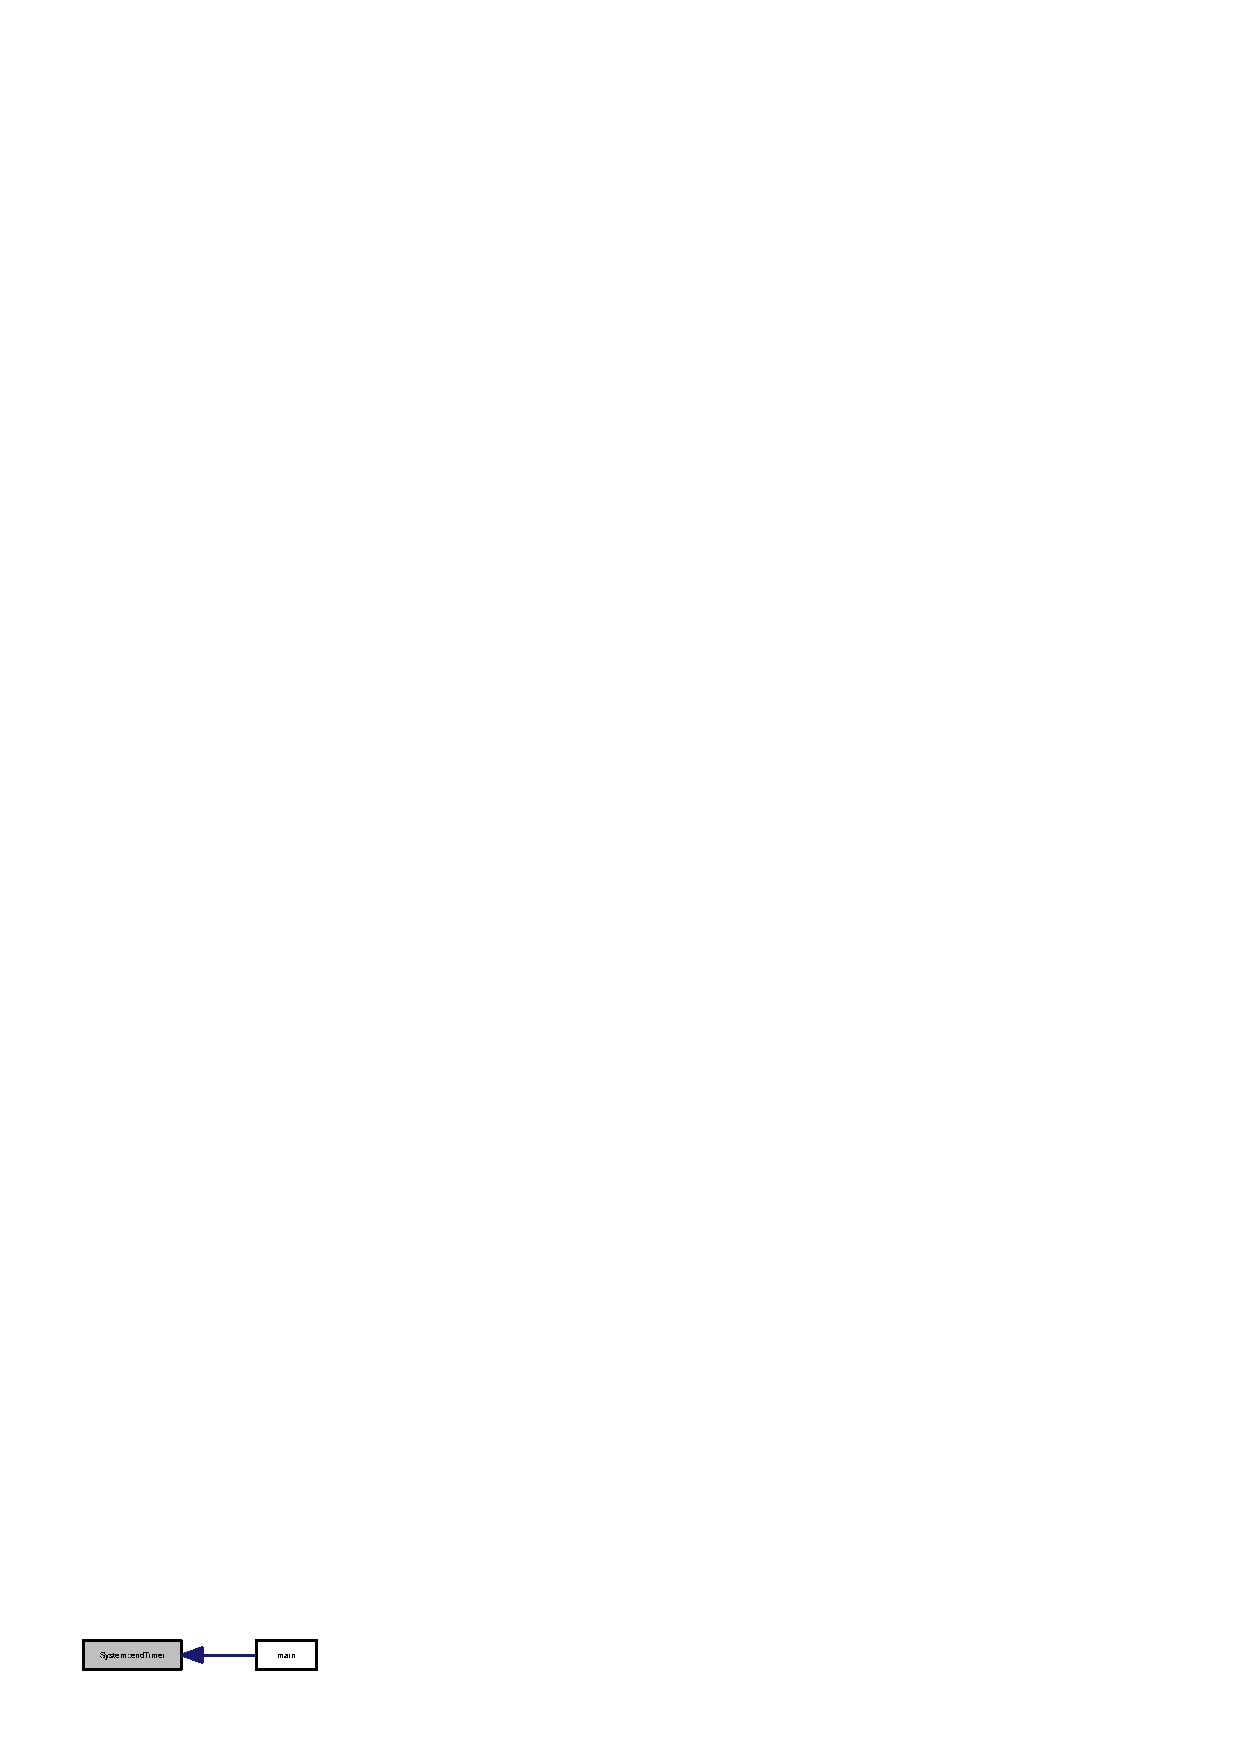
\includegraphics[width=156pt]{class_system_a178a7a315866961f208b6cab6c2d7e88_icgraph}
\end{center}
\end{figure}


\index{System@{System}!get\-Frame\-Rate@{get\-Frame\-Rate}}
\index{get\-Frame\-Rate@{get\-Frame\-Rate}!System@{System}}
\subsubsection[{get\-Frame\-Rate}]{\setlength{\rightskip}{0pt plus 5cm}double System\-::get\-Frame\-Rate (
\begin{DoxyParamCaption}
{}
\end{DoxyParamCaption}
)}\label{class_system_a584a2b655a935ea404937cf8f11ab43c}


フレームレートを取得.\-start\-Timer()とend\-Timer()が実行されていることが前提(c65) 

メソッドget\-Frame\-Rate().フレームレートを取得する(c65)

\begin{DoxyReturn}{戻り値}
time double型.フレームレート取得時間 
\end{DoxyReturn}


 System.\-cpp の 209 行目に定義があります。



参照先 fps, time.



参照元 main().



被呼び出し関係図\-:\nopagebreak
\begin{figure}[H]
\begin{center}
\leavevmode
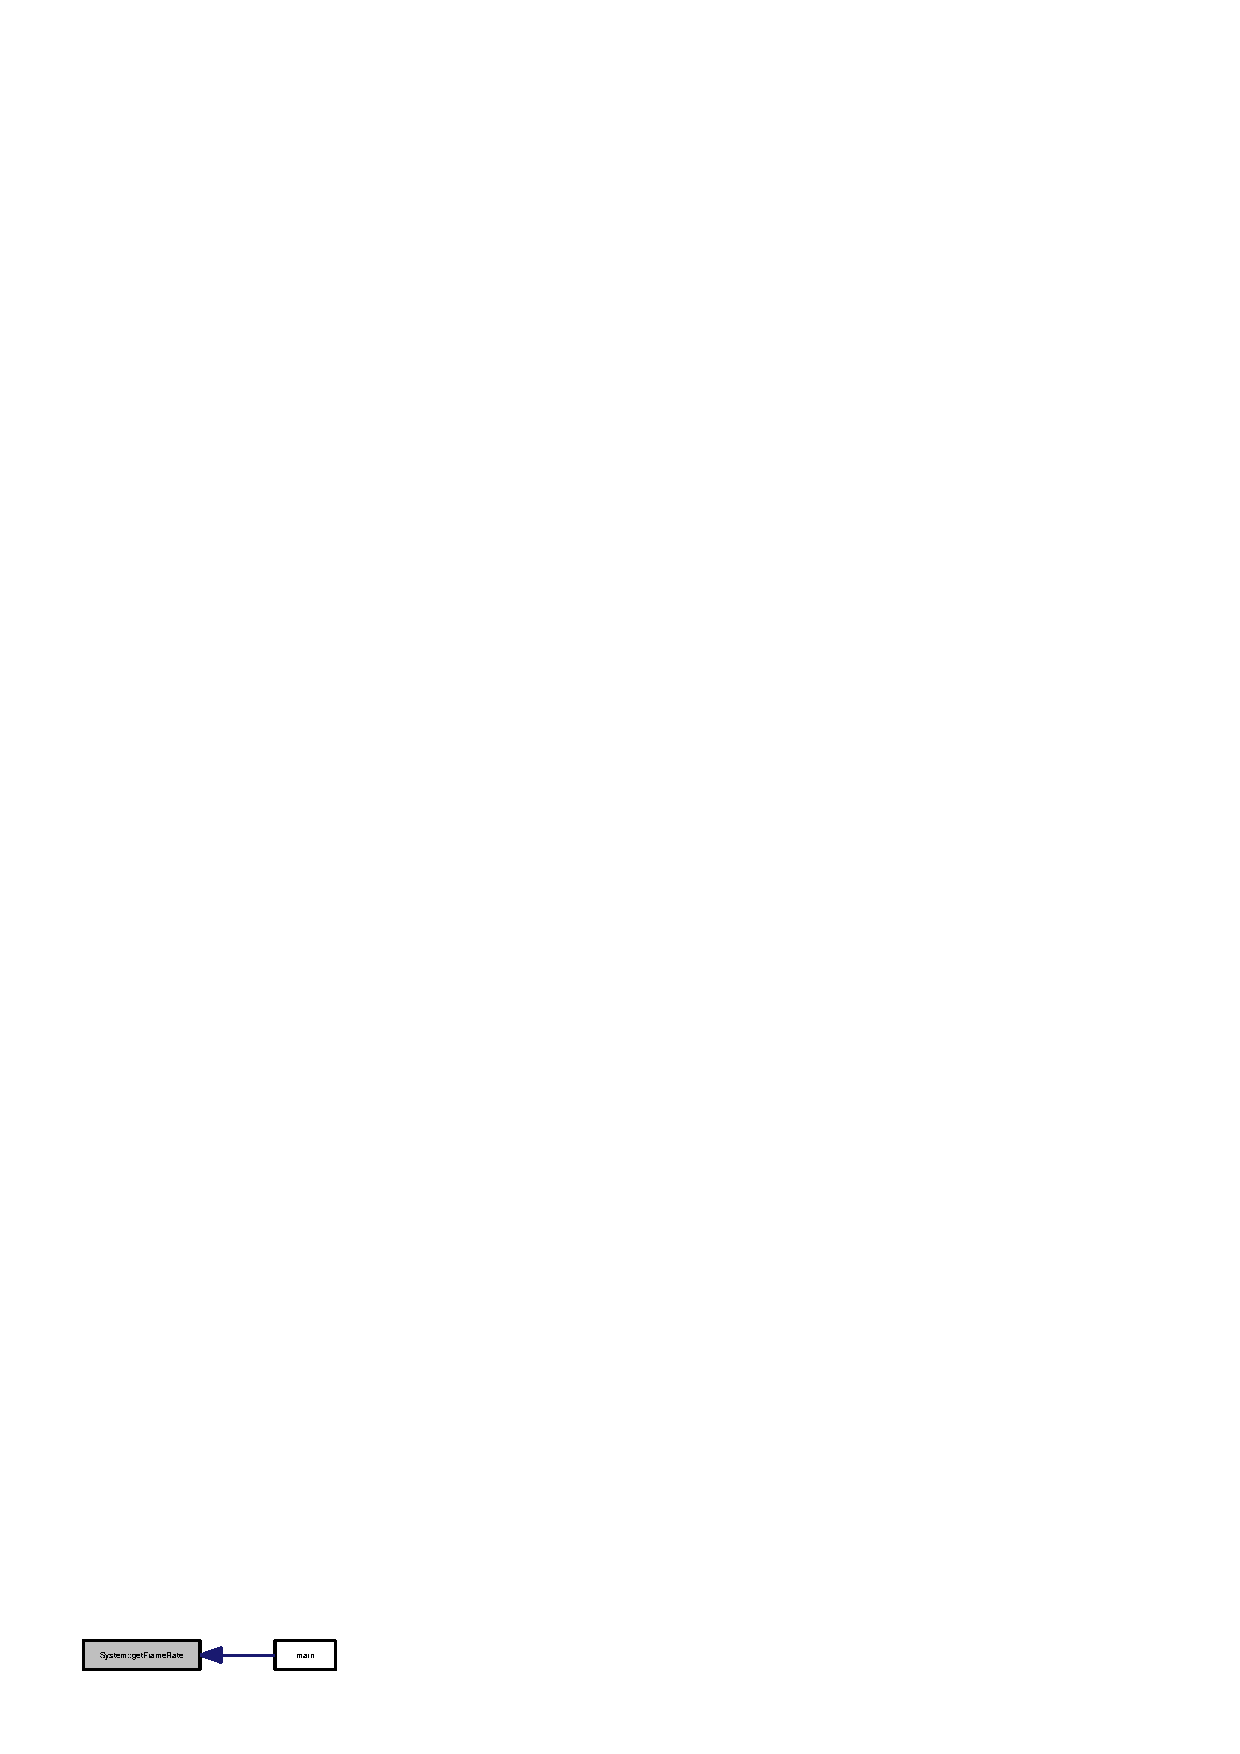
\includegraphics[width=165pt]{class_system_a584a2b655a935ea404937cf8f11ab43c_icgraph}
\end{center}
\end{figure}


\index{System@{System}!get\-Process\-Timein\-Miliseconds@{get\-Process\-Timein\-Miliseconds}}
\index{get\-Process\-Timein\-Miliseconds@{get\-Process\-Timein\-Miliseconds}!System@{System}}
\subsubsection[{get\-Process\-Timein\-Miliseconds}]{\setlength{\rightskip}{0pt plus 5cm}double System\-::get\-Process\-Timein\-Miliseconds (
\begin{DoxyParamCaption}
{}
\end{DoxyParamCaption}
)}\label{class_system_a5f235cfc9736103d150e9dbeee82e543}


計測した時間をミリ秒単位で取得.\-start\-Timer()とend\-Timer()が実行されていることが前提(c65) 

メソッドget\-Time().計測した時間を取得する(c65)

\begin{DoxyReturn}{戻り値}
time double型.処理時間. 
\end{DoxyReturn}


 System.\-cpp の 186 行目に定義があります。



参照先 time.



参照元 main().



被呼び出し関係図\-:\nopagebreak
\begin{figure}[H]
\begin{center}
\leavevmode
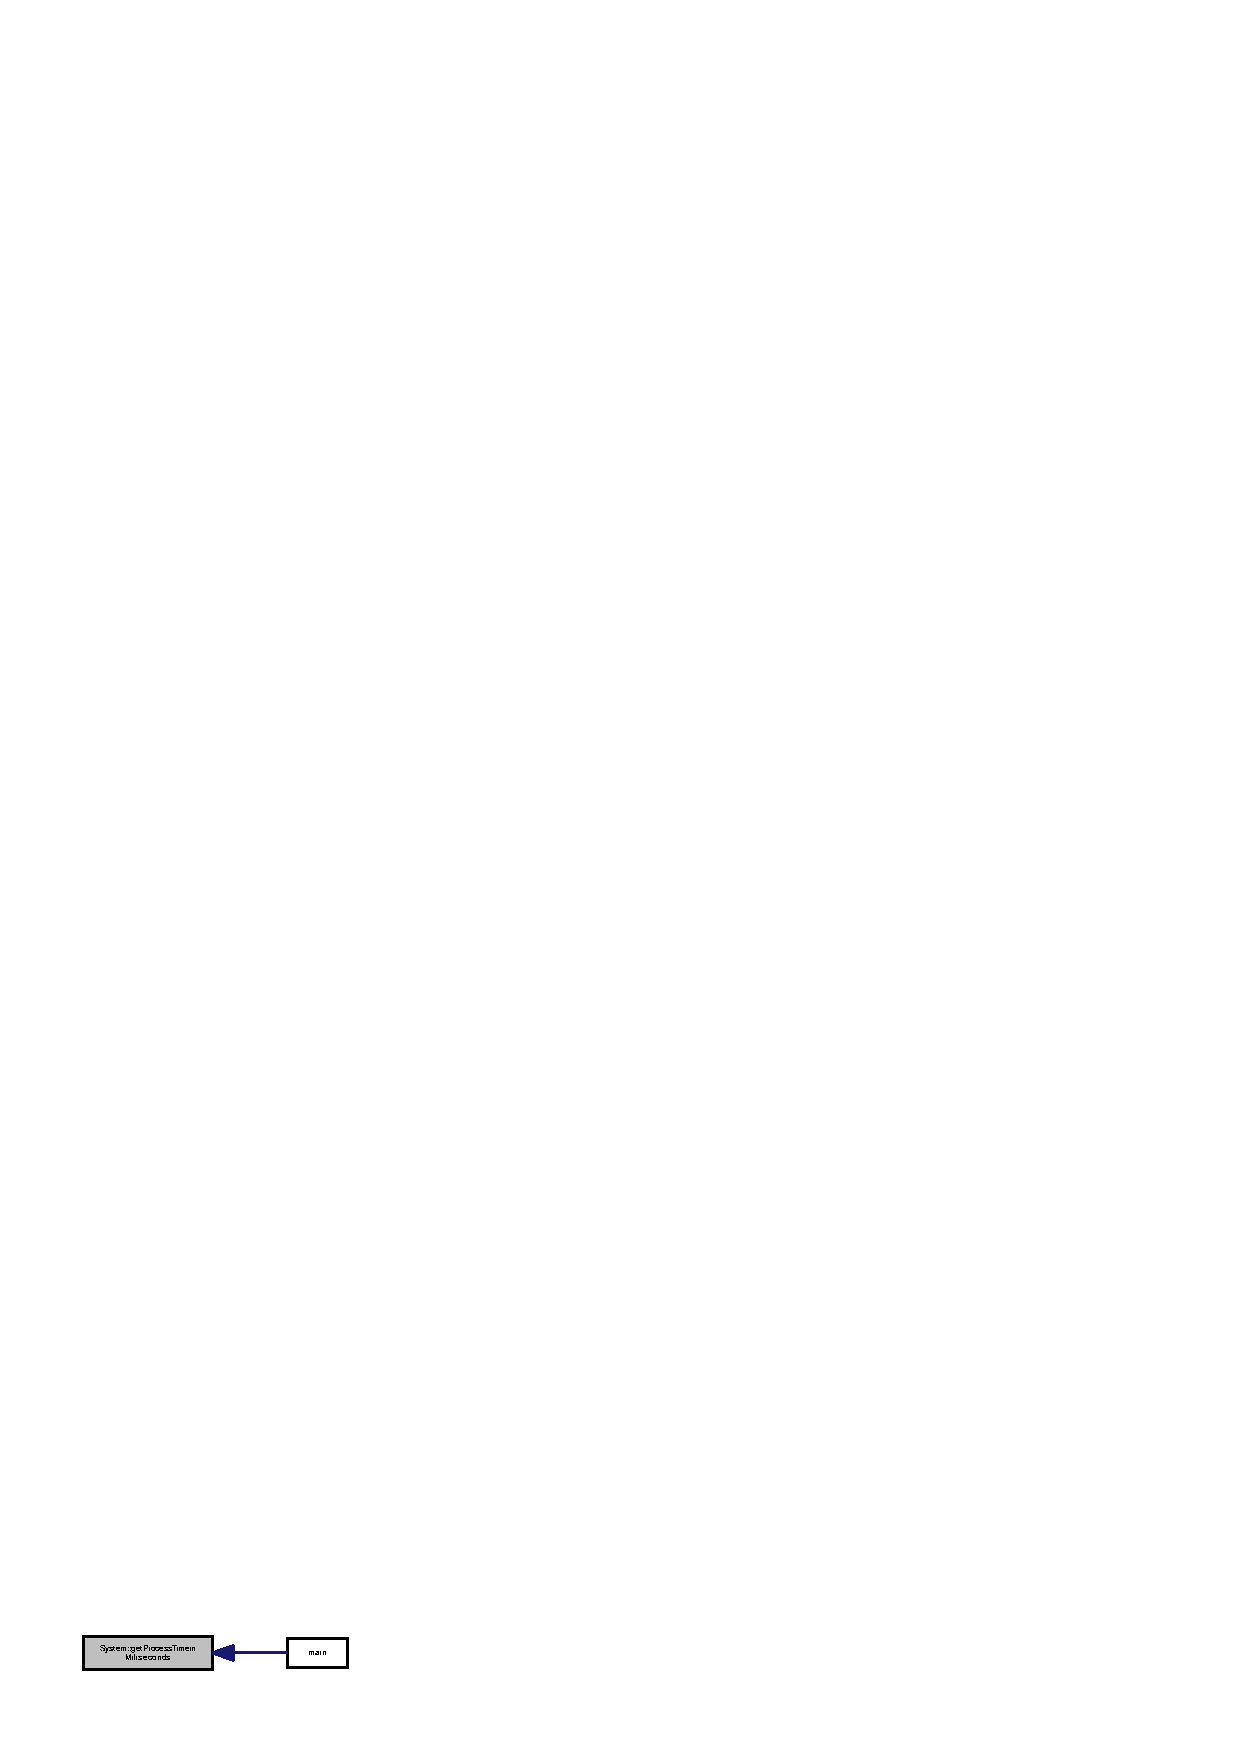
\includegraphics[width=171pt]{class_system_a5f235cfc9736103d150e9dbeee82e543_icgraph}
\end{center}
\end{figure}


\index{System@{System}!make\-Directory@{make\-Directory}}
\index{make\-Directory@{make\-Directory}!System@{System}}
\subsubsection[{make\-Directory}]{\setlength{\rightskip}{0pt plus 5cm}void System\-::make\-Directory (
\begin{DoxyParamCaption}
\item[{char $\ast$}]{original\-\_\-path, }
\item[{int}]{create\-\_\-dirnum}
\end{DoxyParamCaption}
)}\label{class_system_a4e8e357a7875f40a86cee5cfdad6b6ed}


指定したディレクトリ以下に新しいディレクトリを作成する( 

\doxyref{System\-::make\-Directory()}{p.}{class_system_a4e8e357a7875f40a86cee5cfdad6b6ed}.指定したディレクトリ以下に新しいディレクトリを作成する


\begin{DoxyParams}{引数}
{\em original\-\_\-path} & char$\ast$型.指定したベースとなるディレクトリ \\
\hline
{\em create\-\_\-dirnum} & int型.ディレクトリ番号 \\
\hline
\end{DoxyParams}


 System.\-cpp の 266 行目に定義があります。



参照先 N\-O\-C.



参照元 main().



被呼び出し関係図\-:\nopagebreak
\begin{figure}[H]
\begin{center}
\leavevmode
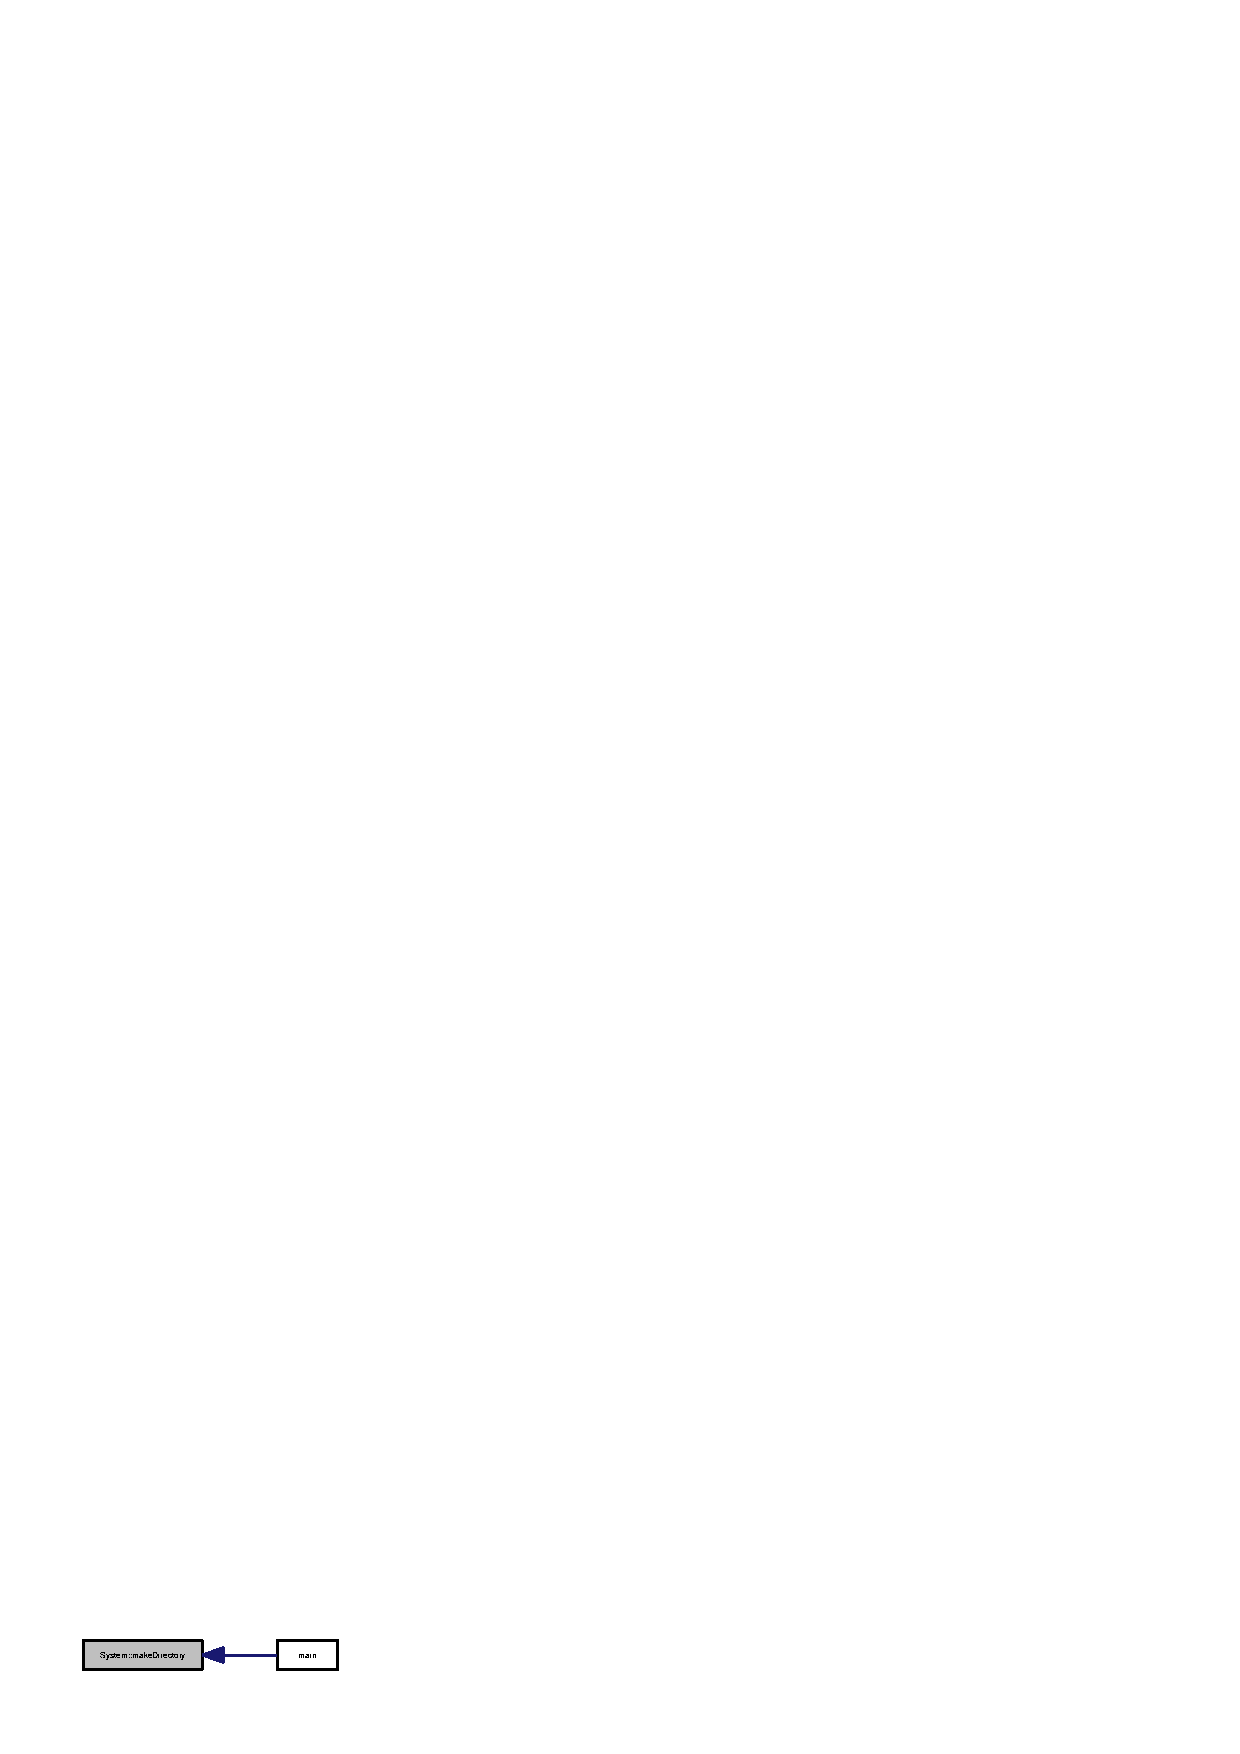
\includegraphics[width=166pt]{class_system_a4e8e357a7875f40a86cee5cfdad6b6ed_icgraph}
\end{center}
\end{figure}


\index{System@{System}!make\-Directory\-Based\-Date@{make\-Directory\-Based\-Date}}
\index{make\-Directory\-Based\-Date@{make\-Directory\-Based\-Date}!System@{System}}
\subsubsection[{make\-Directory\-Based\-Date}]{\setlength{\rightskip}{0pt plus 5cm}void System\-::make\-Directory\-Based\-Date (
\begin{DoxyParamCaption}
{}
\end{DoxyParamCaption}
)}\label{class_system_a6353709a74c9a12a3b1c8e365db5f51e}


日付に基づいたディレクトリの作成 

\doxyref{System\-::make\-Directory()}{p.}{class_system_a4e8e357a7875f40a86cee5cfdad6b6ed}.ディレクトリを作成 

 System.\-cpp の 247 行目に定義があります。



参照先 directory\-Name, N\-O\-C.



参照元 main().



被呼び出し関係図\-:\nopagebreak
\begin{figure}[H]
\begin{center}
\leavevmode
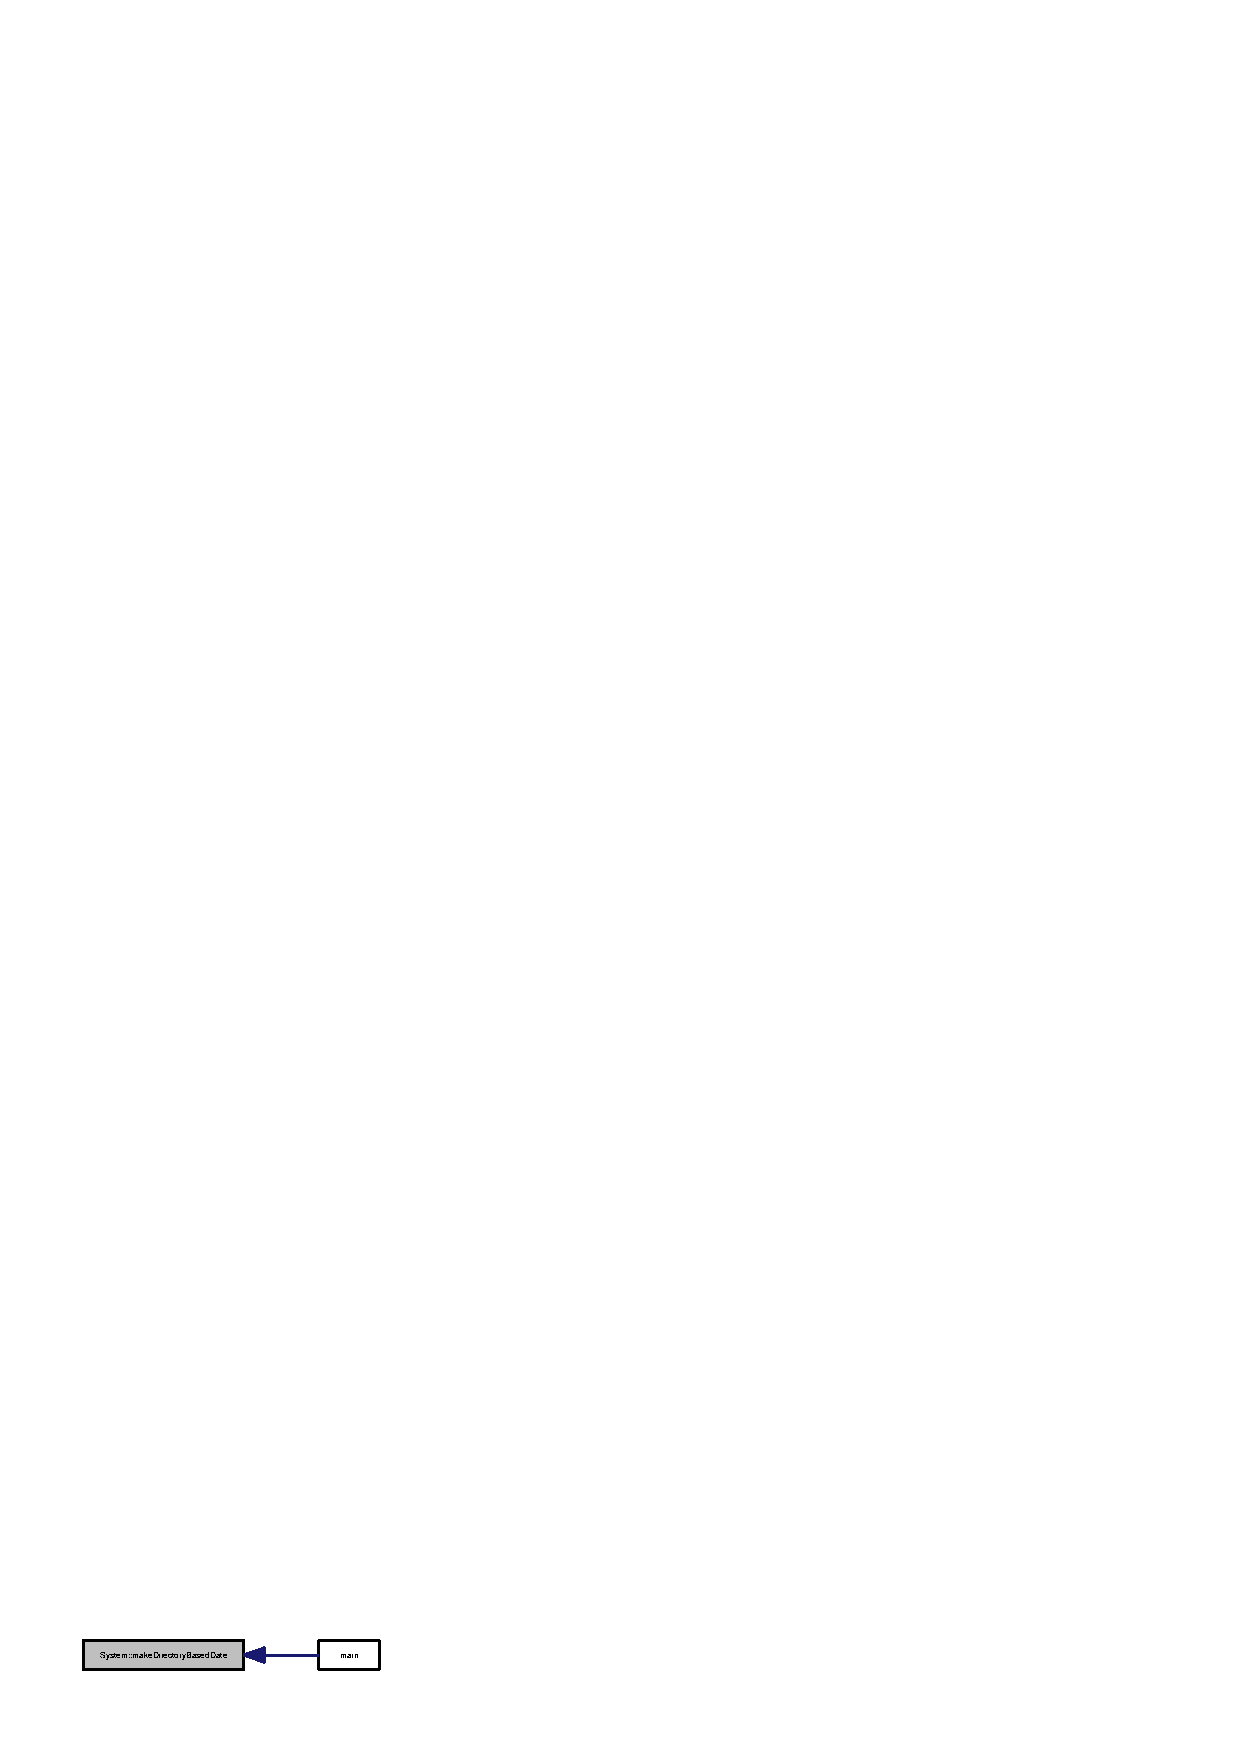
\includegraphics[width=186pt]{class_system_a6353709a74c9a12a3b1c8e365db5f51e_icgraph}
\end{center}
\end{figure}


\index{System@{System}!open\-Directory@{open\-Directory}}
\index{open\-Directory@{open\-Directory}!System@{System}}
\subsubsection[{open\-Directory}]{\setlength{\rightskip}{0pt plus 5cm}void System\-::open\-Directory (
\begin{DoxyParamCaption}
{}
\end{DoxyParamCaption}
)}\label{class_system_a9016157380cb3dfe6637731daf2e3b4b}


ディレクトリを開く(c38) 

System\-::open\-Direectory().出力したディレクトリを開く(c39) 

 System.\-cpp の 324 行目に定義があります。



参照先 directory\-Name, N\-O\-C.



参照元 end\-Message().



被呼び出し関係図\-:\nopagebreak
\begin{figure}[H]
\begin{center}
\leavevmode
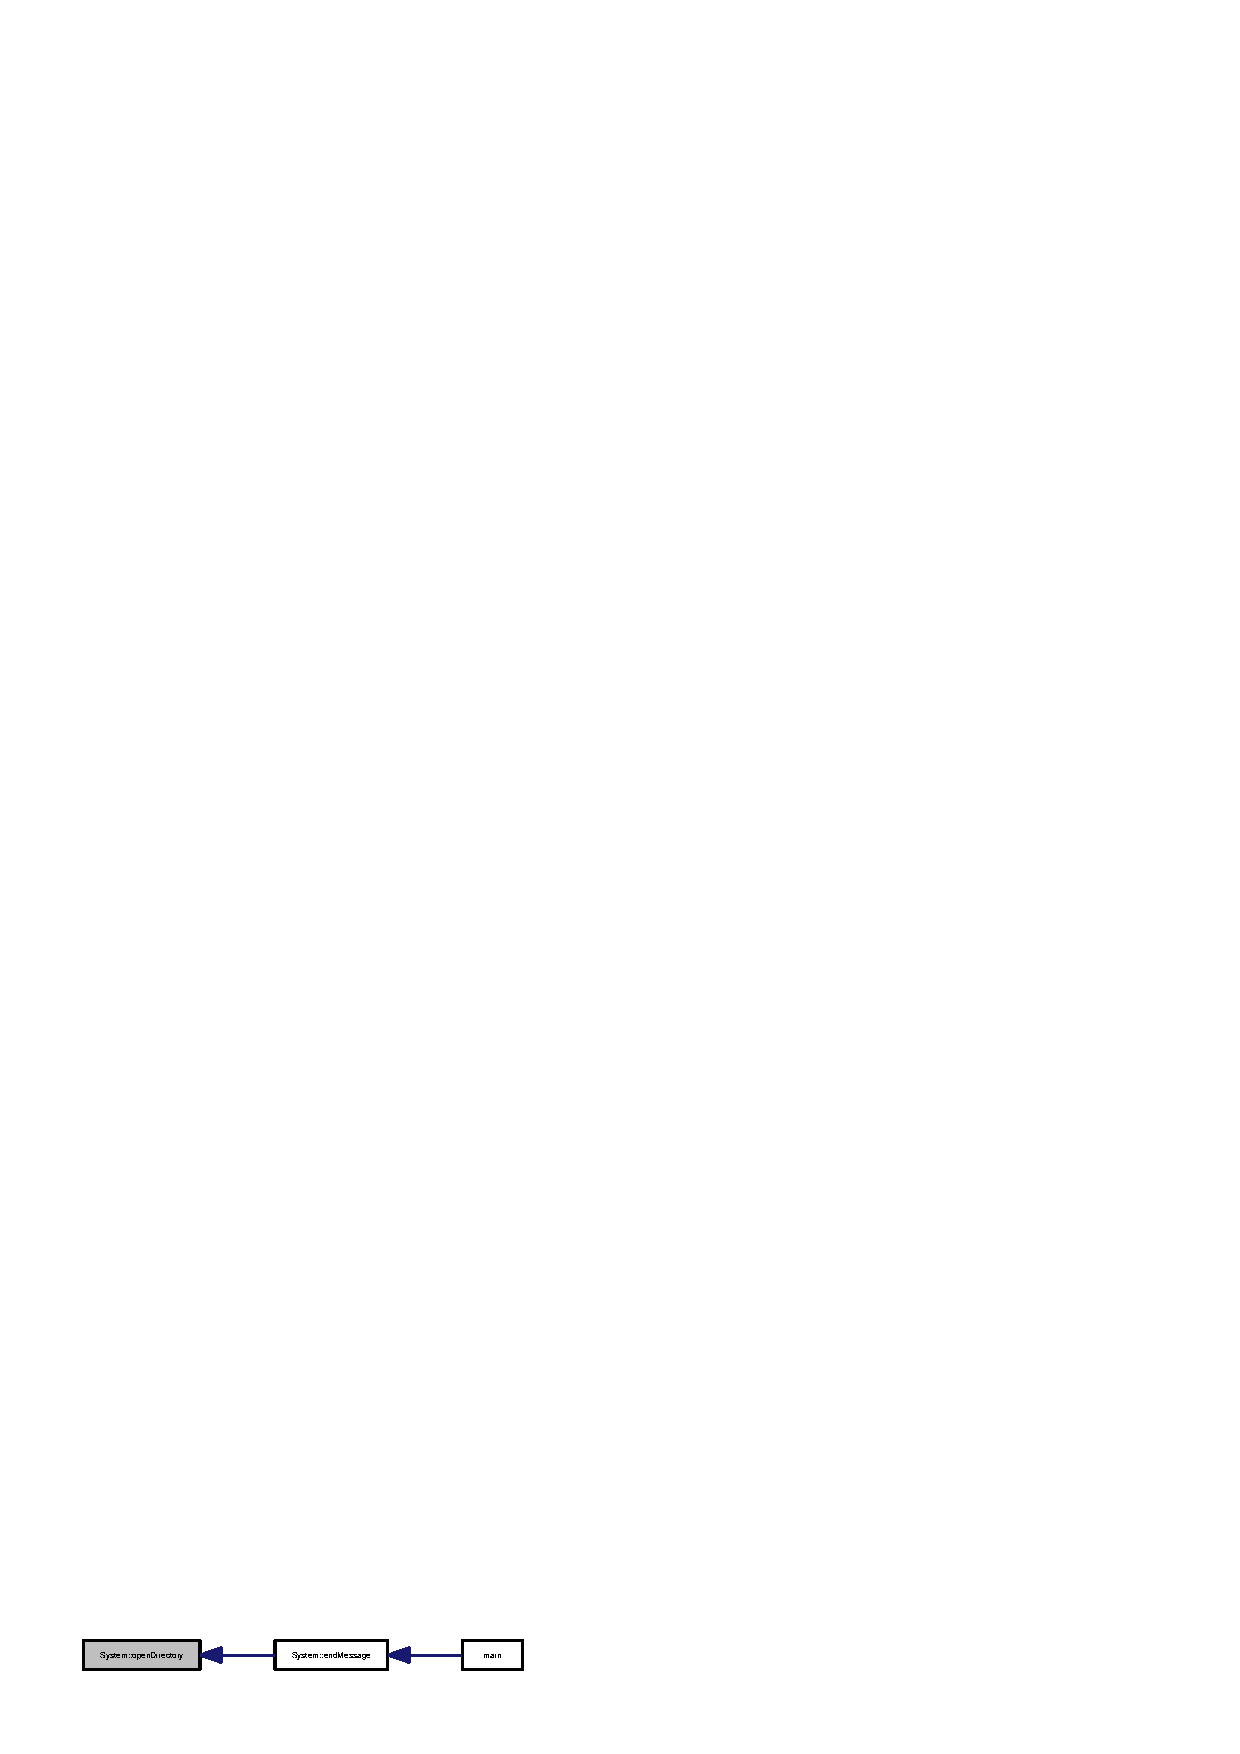
\includegraphics[width=255pt]{class_system_a9016157380cb3dfe6637731daf2e3b4b_icgraph}
\end{center}
\end{figure}


\index{System@{System}!output\-Video@{output\-Video}}
\index{output\-Video@{output\-Video}!System@{System}}
\subsubsection[{output\-Video}]{\setlength{\rightskip}{0pt plus 5cm}Video\-Writer System\-::output\-Video (
\begin{DoxyParamCaption}
\item[{const string $\ast$}]{output\-Video\-Name}
\end{DoxyParamCaption}
)}\label{class_system_a95bbdc3e7877f2d919f4d92dc4a79367}


動画を出力する 

\doxyref{System\-::output\-Video()}{p.}{class_system_a95bbdc3e7877f2d919f4d92dc4a79367}.動作確認用に動画を出力するメソッド


\begin{DoxyParams}{引数}
{\em output\-Video\-Name} & const string$\ast$型.出力したい動画のファイル名 \\
\hline
\end{DoxyParams}
\begin{DoxyReturn}{戻り値}
writer Video\-Writer型.出力する動画の情報 
\end{DoxyReturn}
$<$動画出力時のパス(c38) 

 System.\-cpp の 339 行目に定義があります。



参照先 directory\-Name, N\-O\-C.

\index{System@{System}!remove\-Directory@{remove\-Directory}}
\index{remove\-Directory@{remove\-Directory}!System@{System}}
\subsubsection[{remove\-Directory}]{\setlength{\rightskip}{0pt plus 5cm}void System\-::remove\-Directory (
\begin{DoxyParamCaption}
{}
\end{DoxyParamCaption}
)}\label{class_system_a3523df6c59162a85350b41a065efa3dd}


取得したデータが不要だった場合ディレクトリを削除する 

\doxyref{System\-::remove\-Directory()}{p.}{class_system_a3523df6c59162a85350b41a065efa3dd}.ディレクトリを削除(c21) 

 System.\-cpp の 278 行目に定義があります。



参照先 directory\-Name, N\-O\-C.



参照元 main().



被呼び出し関係図\-:\nopagebreak
\begin{figure}[H]
\begin{center}
\leavevmode
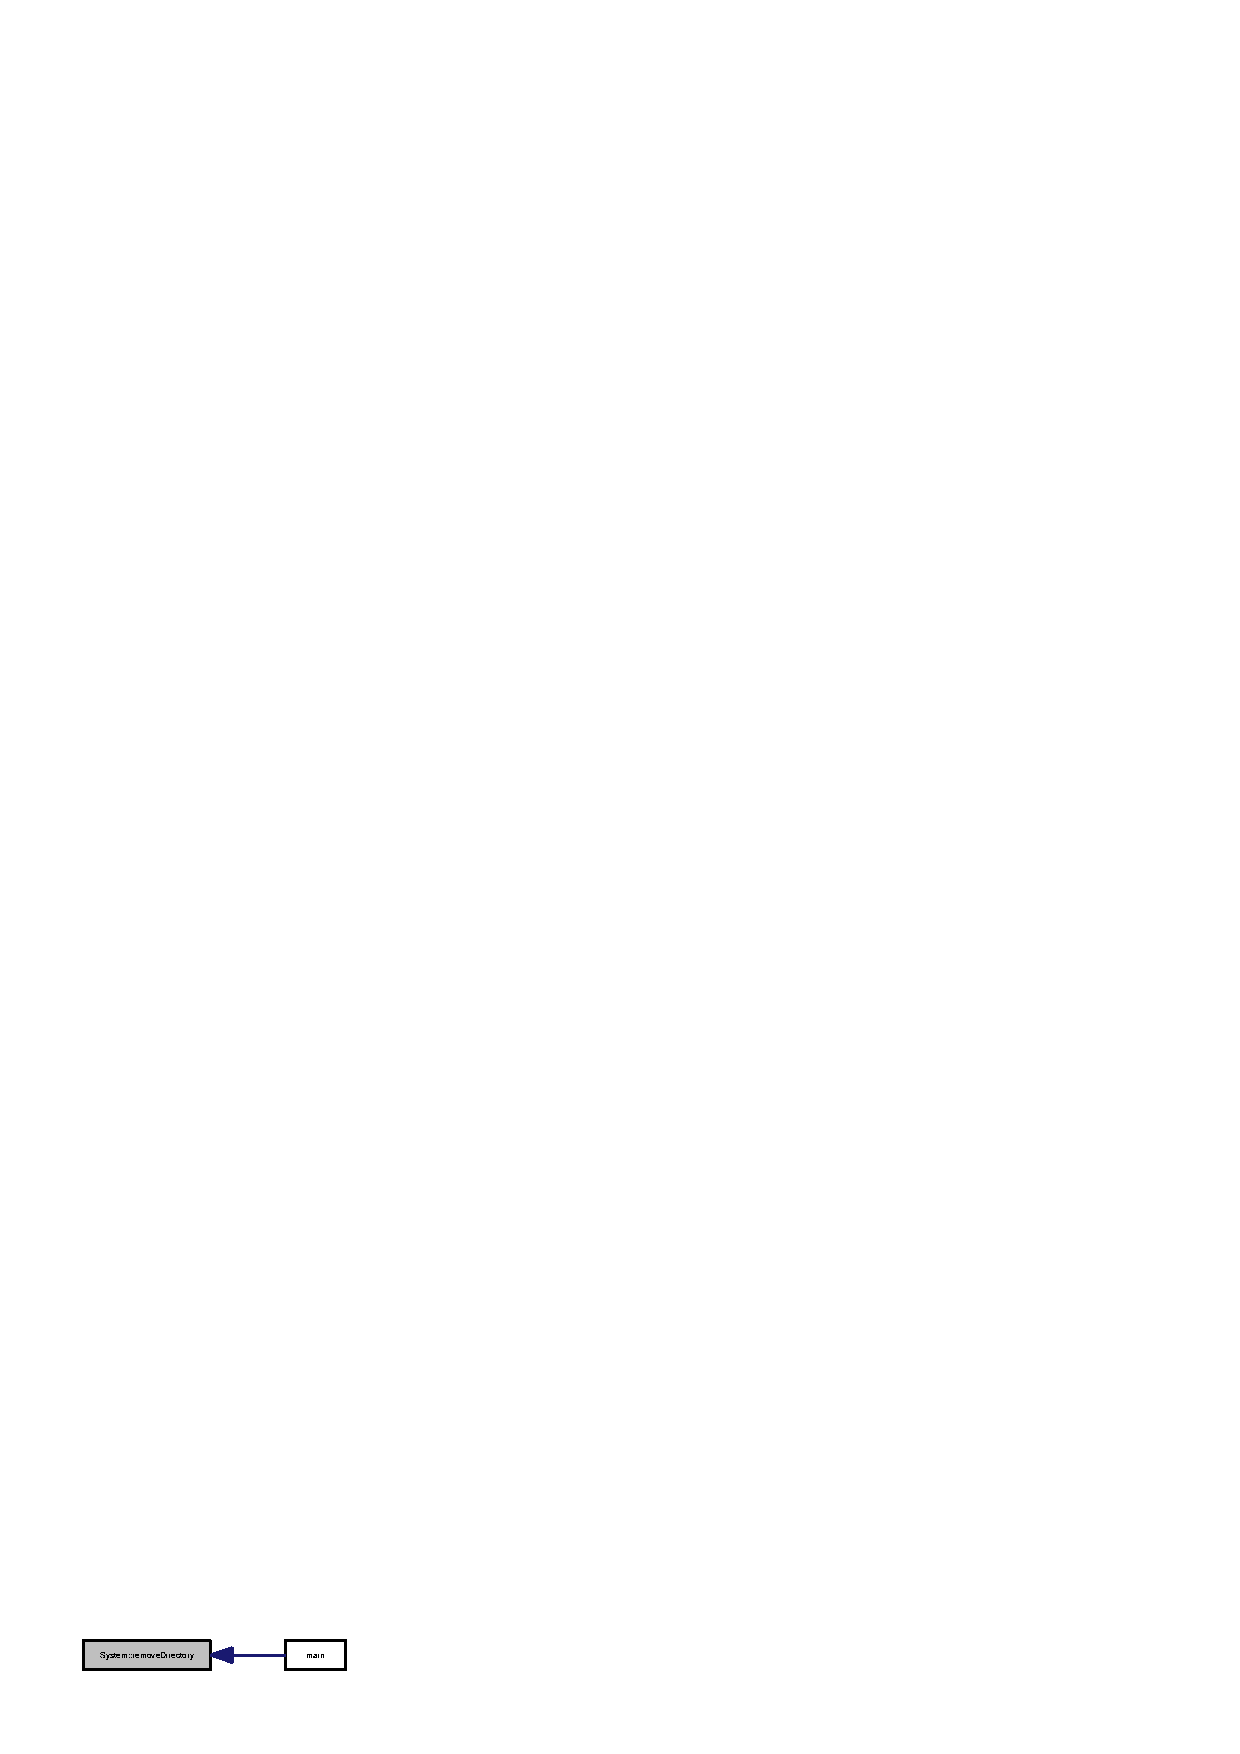
\includegraphics[width=170pt]{class_system_a3523df6c59162a85350b41a065efa3dd_icgraph}
\end{center}
\end{figure}


\index{System@{System}!show\-Help\-Message@{show\-Help\-Message}}
\index{show\-Help\-Message@{show\-Help\-Message}!System@{System}}
\subsubsection[{show\-Help\-Message}]{\setlength{\rightskip}{0pt plus 5cm}void System\-::show\-Help\-Message (
\begin{DoxyParamCaption}
{}
\end{DoxyParamCaption}
)}\label{class_system_af0fc7b12dc7342e2109a9aa3894b9bbe}


キー入力に関するヘルプを表示(c86) 

メソッド\-System\-::show\-Help\-Message().ヘルプメッセージを表示する 

 System.\-cpp の 87 行目に定義があります。



参照元 main().



被呼び出し関係図\-:\nopagebreak
\begin{figure}[H]
\begin{center}
\leavevmode
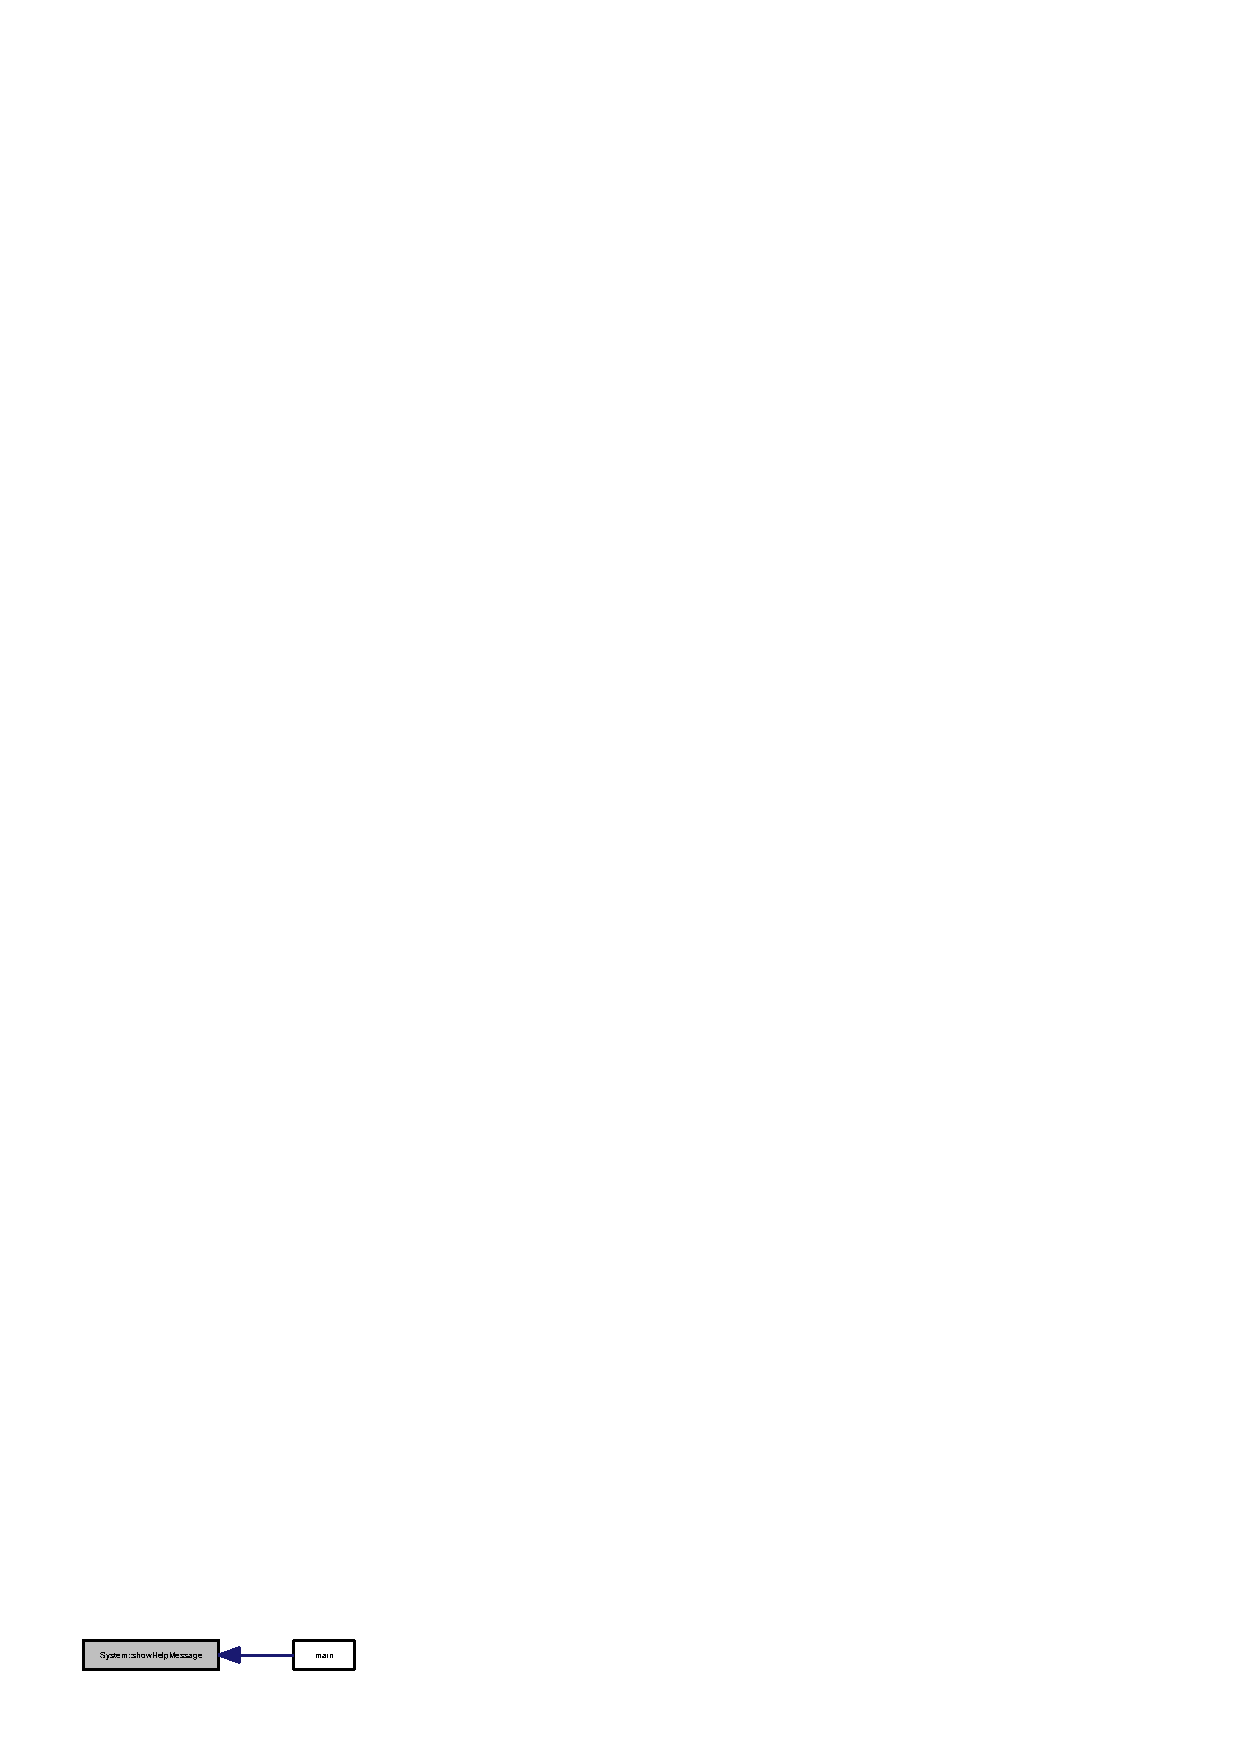
\includegraphics[width=174pt]{class_system_af0fc7b12dc7342e2109a9aa3894b9bbe_icgraph}
\end{center}
\end{figure}


\index{System@{System}!start\-Message@{start\-Message}}
\index{start\-Message@{start\-Message}!System@{System}}
\subsubsection[{start\-Message}]{\setlength{\rightskip}{0pt plus 5cm}void System\-::start\-Message (
\begin{DoxyParamCaption}
{}
\end{DoxyParamCaption}
)}\label{class_system_a15325f6b106b804af8432d102945535c}


プログラム開始時のメッセージを表示(c26) 

\doxyref{System\-::start\-Message()}{p.}{class_system_a15325f6b106b804af8432d102945535c}.プログラム起動時のメッセージ 

 System.\-cpp の 36 行目に定義があります。



参照元 main().



被呼び出し関係図\-:\nopagebreak
\begin{figure}[H]
\begin{center}
\leavevmode
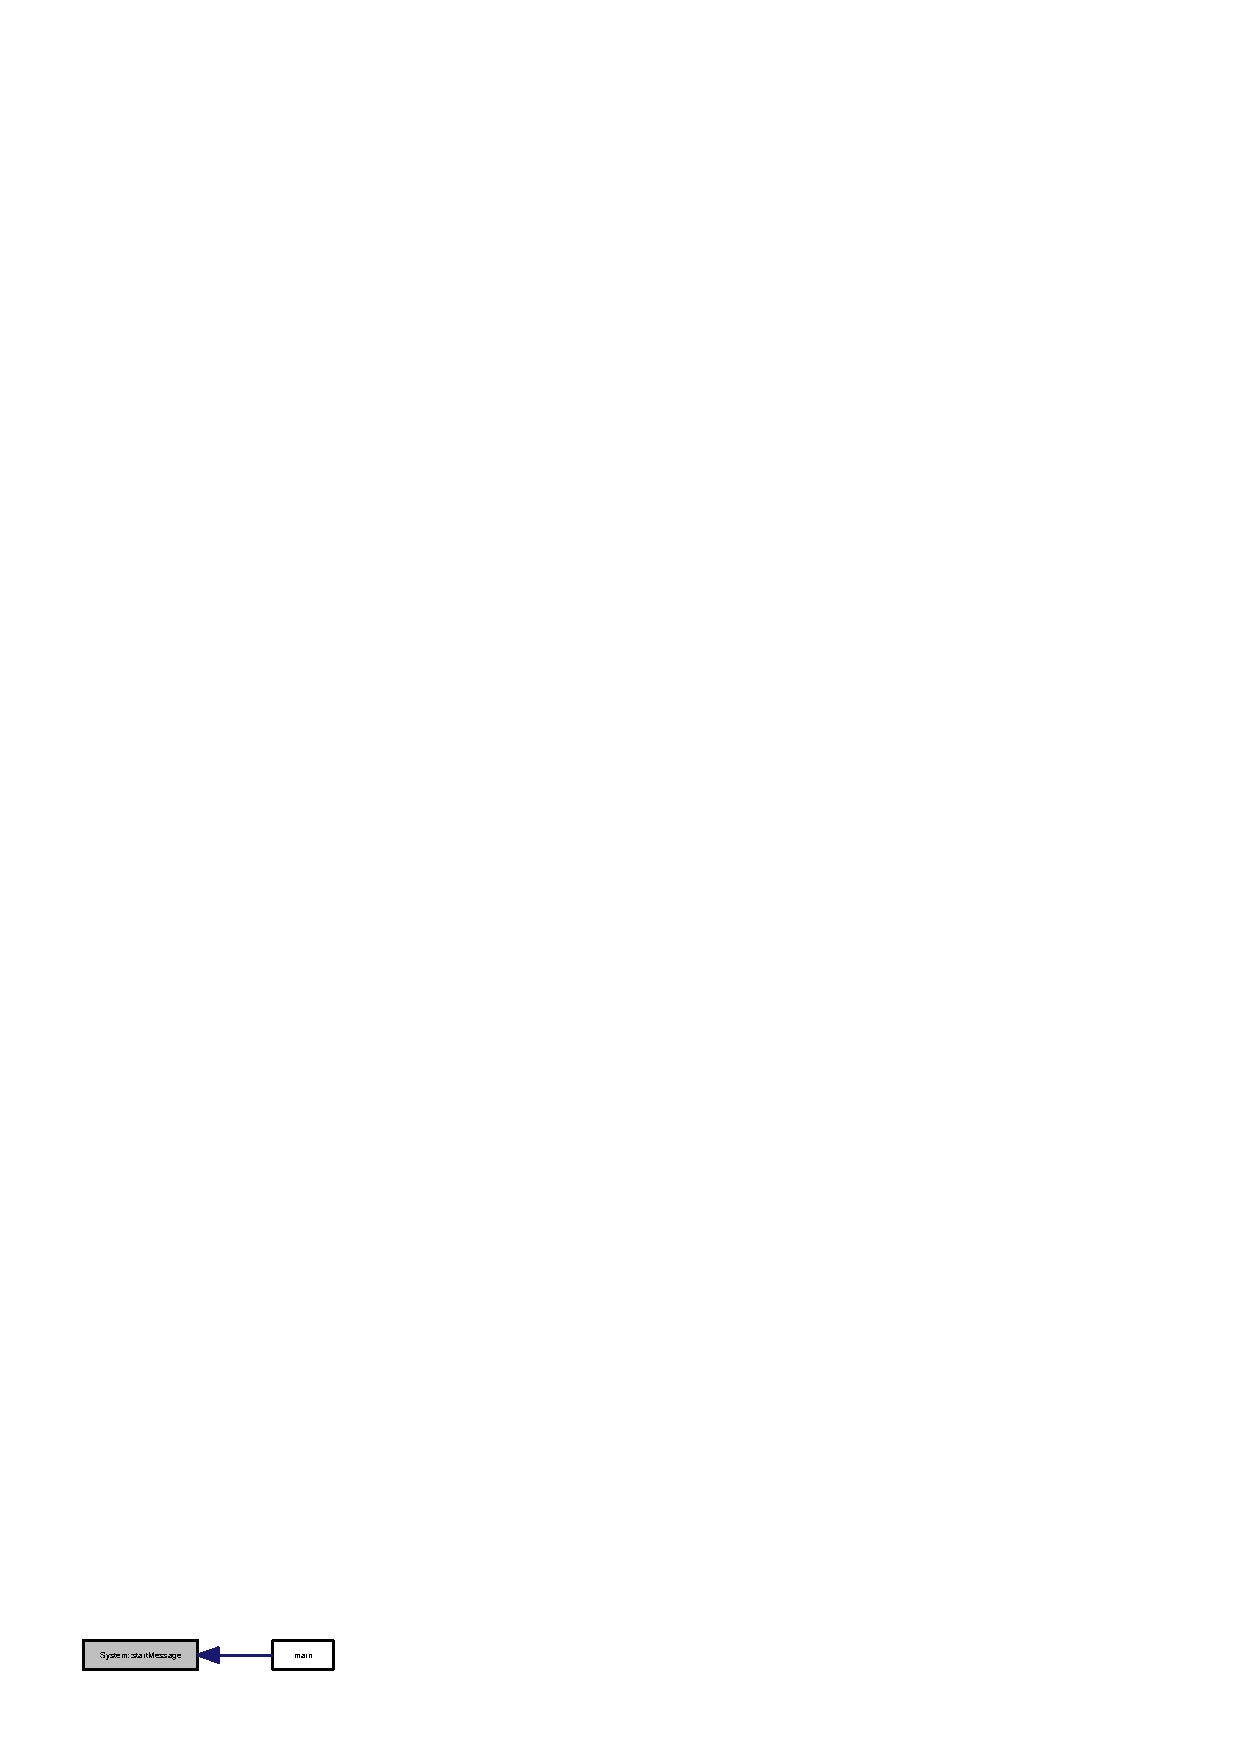
\includegraphics[width=164pt]{class_system_a15325f6b106b804af8432d102945535c_icgraph}
\end{center}
\end{figure}


\index{System@{System}!start\-Timer@{start\-Timer}}
\index{start\-Timer@{start\-Timer}!System@{System}}
\subsubsection[{start\-Timer}]{\setlength{\rightskip}{0pt plus 5cm}void System\-::start\-Timer (
\begin{DoxyParamCaption}
{}
\end{DoxyParamCaption}
)}\label{class_system_ac62488af6f94b96aa37988c54e19074f}


タイマーを開始(c65) 

メソッドstart\-Timer().タイマーを開始する 

 System.\-cpp の 157 行目に定義があります。



参照元 main().



被呼び出し関係図\-:\nopagebreak
\begin{figure}[H]
\begin{center}
\leavevmode
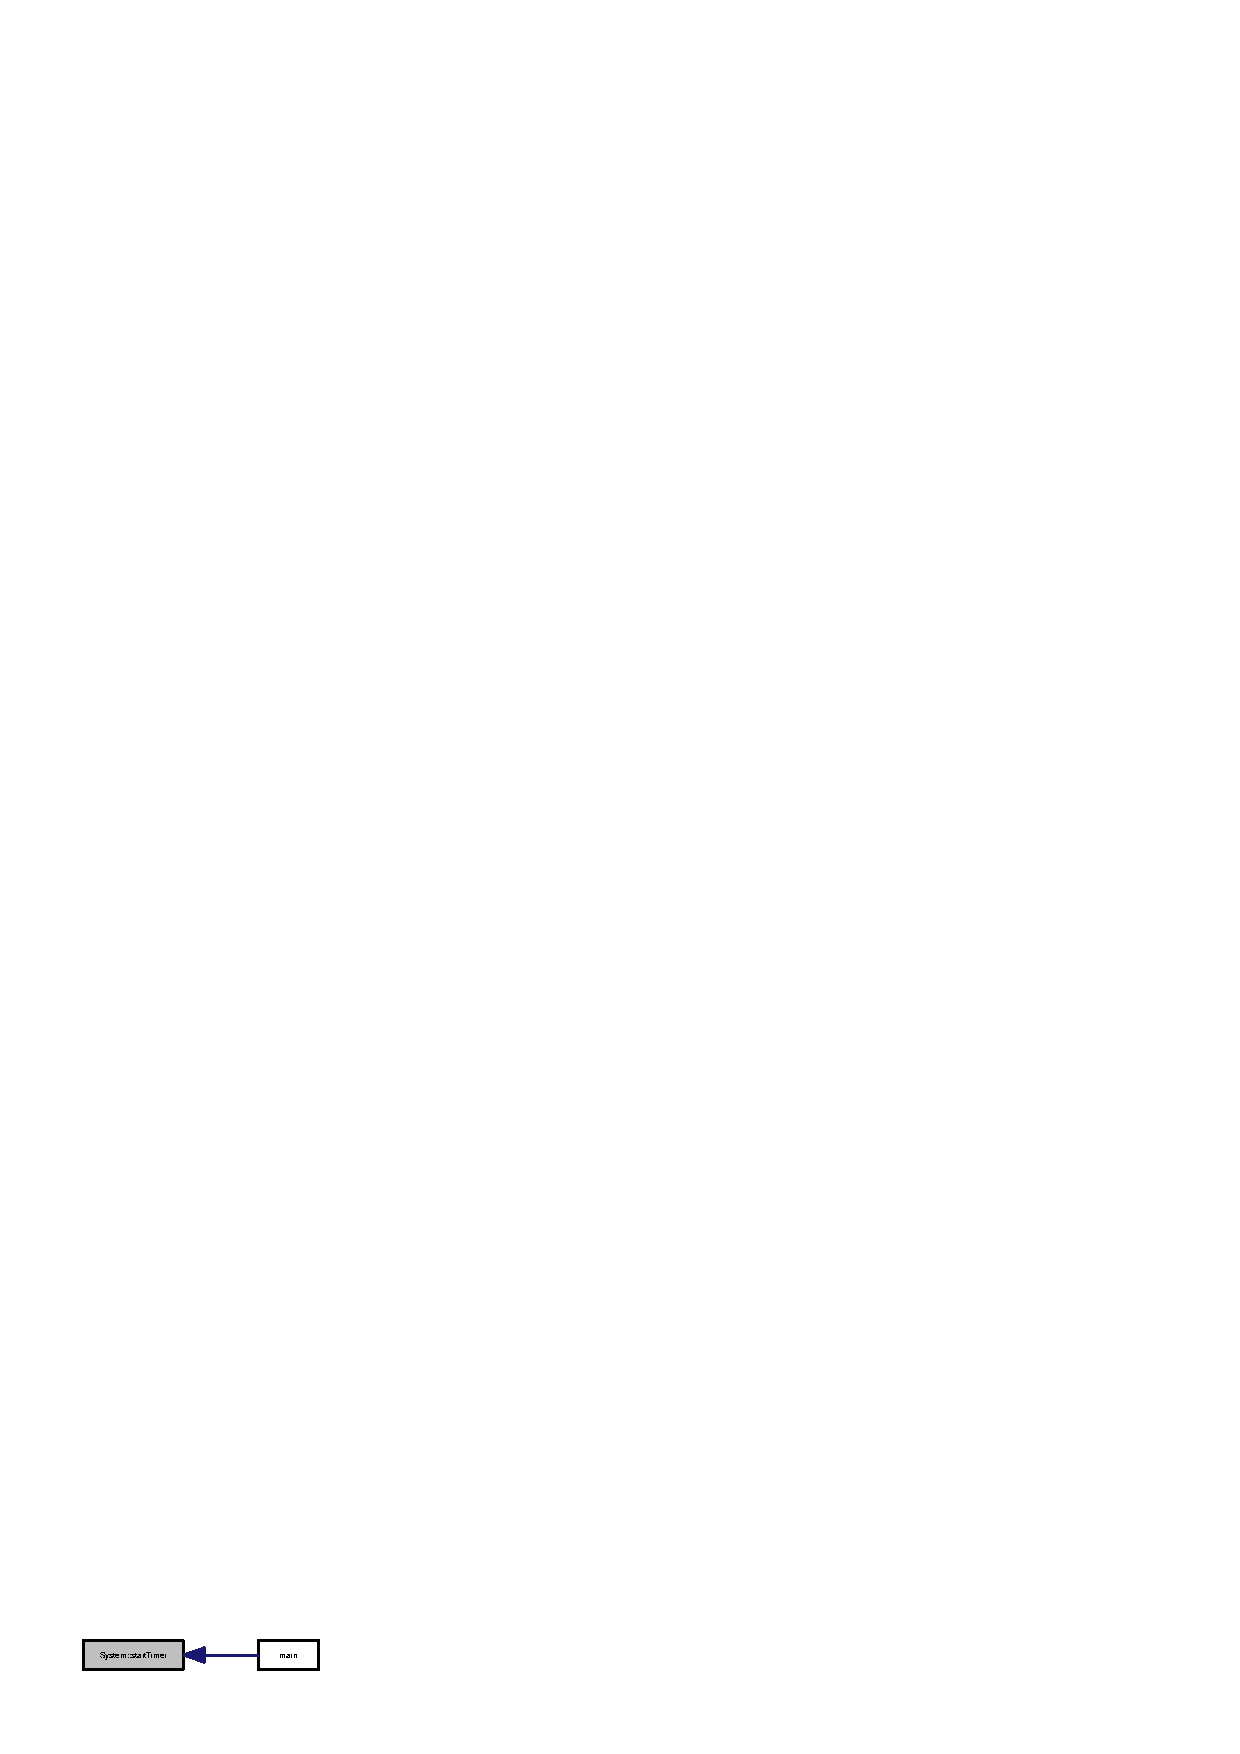
\includegraphics[width=157pt]{class_system_ac62488af6f94b96aa37988c54e19074f_icgraph}
\end{center}
\end{figure}




\subsection{メンバ詳解}
\index{System@{System}!fps@{fps}}
\index{fps@{fps}!System@{System}}
\subsubsection[{fps}]{\setlength{\rightskip}{0pt plus 5cm}double System\-::fps}\label{class_system_a1339ce8aca0b83646a5879b4068c4ddb}


フレームレート 



 System.\-hpp の 45 行目に定義があります。



参照元 get\-Frame\-Rate(), System().

\index{System@{System}!sum\-\_\-time@{sum\-\_\-time}}
\index{sum\-\_\-time@{sum\-\_\-time}!System@{System}}
\subsubsection[{sum\-\_\-time}]{\setlength{\rightskip}{0pt plus 5cm}double System\-::sum\-\_\-time}\label{class_system_aab7a0fe9f9f094ab4462a6f0e5765d92}


処理の合計時間 



 System.\-hpp の 46 行目に定義があります。



参照元 main(), System().

\index{System@{System}!time@{time}}
\index{time@{time}!System@{System}}
\subsubsection[{time}]{\setlength{\rightskip}{0pt plus 5cm}double System\-::time}\label{class_system_aa9e002a5f2f169e37c545b76ee67e724}


処理時間の結果 



 System.\-hpp の 44 行目に定義があります。



参照元 end\-Timer(), get\-Frame\-Rate(), get\-Process\-Timein\-Miliseconds(), System().



このクラス詳解は次のファイルから抽出されました\-:\begin{DoxyCompactItemize}
\item 
{\bf System.\-hpp}\item 
{\bf System.\-cpp}\end{DoxyCompactItemize}

\chapter{ファイル詳解}
\section{Drawing.\-cpp ファイル}
\label{_drawing_8cpp}\index{Drawing.\-cpp@{Drawing.\-cpp}}
{\ttfamily \#include \char`\"{}Path\-Tracking\-And\-Induction\-Of\-The\-Robot.\-hpp\char`\"{}}\\*
{\ttfamily \#include \char`\"{}Drawing.\-hpp\char`\"{}}\\*

\section{Drawing.\-hpp ファイル}
\label{_drawing_8hpp}\index{Drawing.\-hpp@{Drawing.\-hpp}}
{\ttfamily \#include \char`\"{}Path\-Tracking\-And\-Induction\-Of\-The\-Robot.\-hpp\char`\"{}}\\*
Drawing.\-hpp の依存先関係図\-:\nopagebreak
\begin{figure}[H]
\begin{center}
\leavevmode
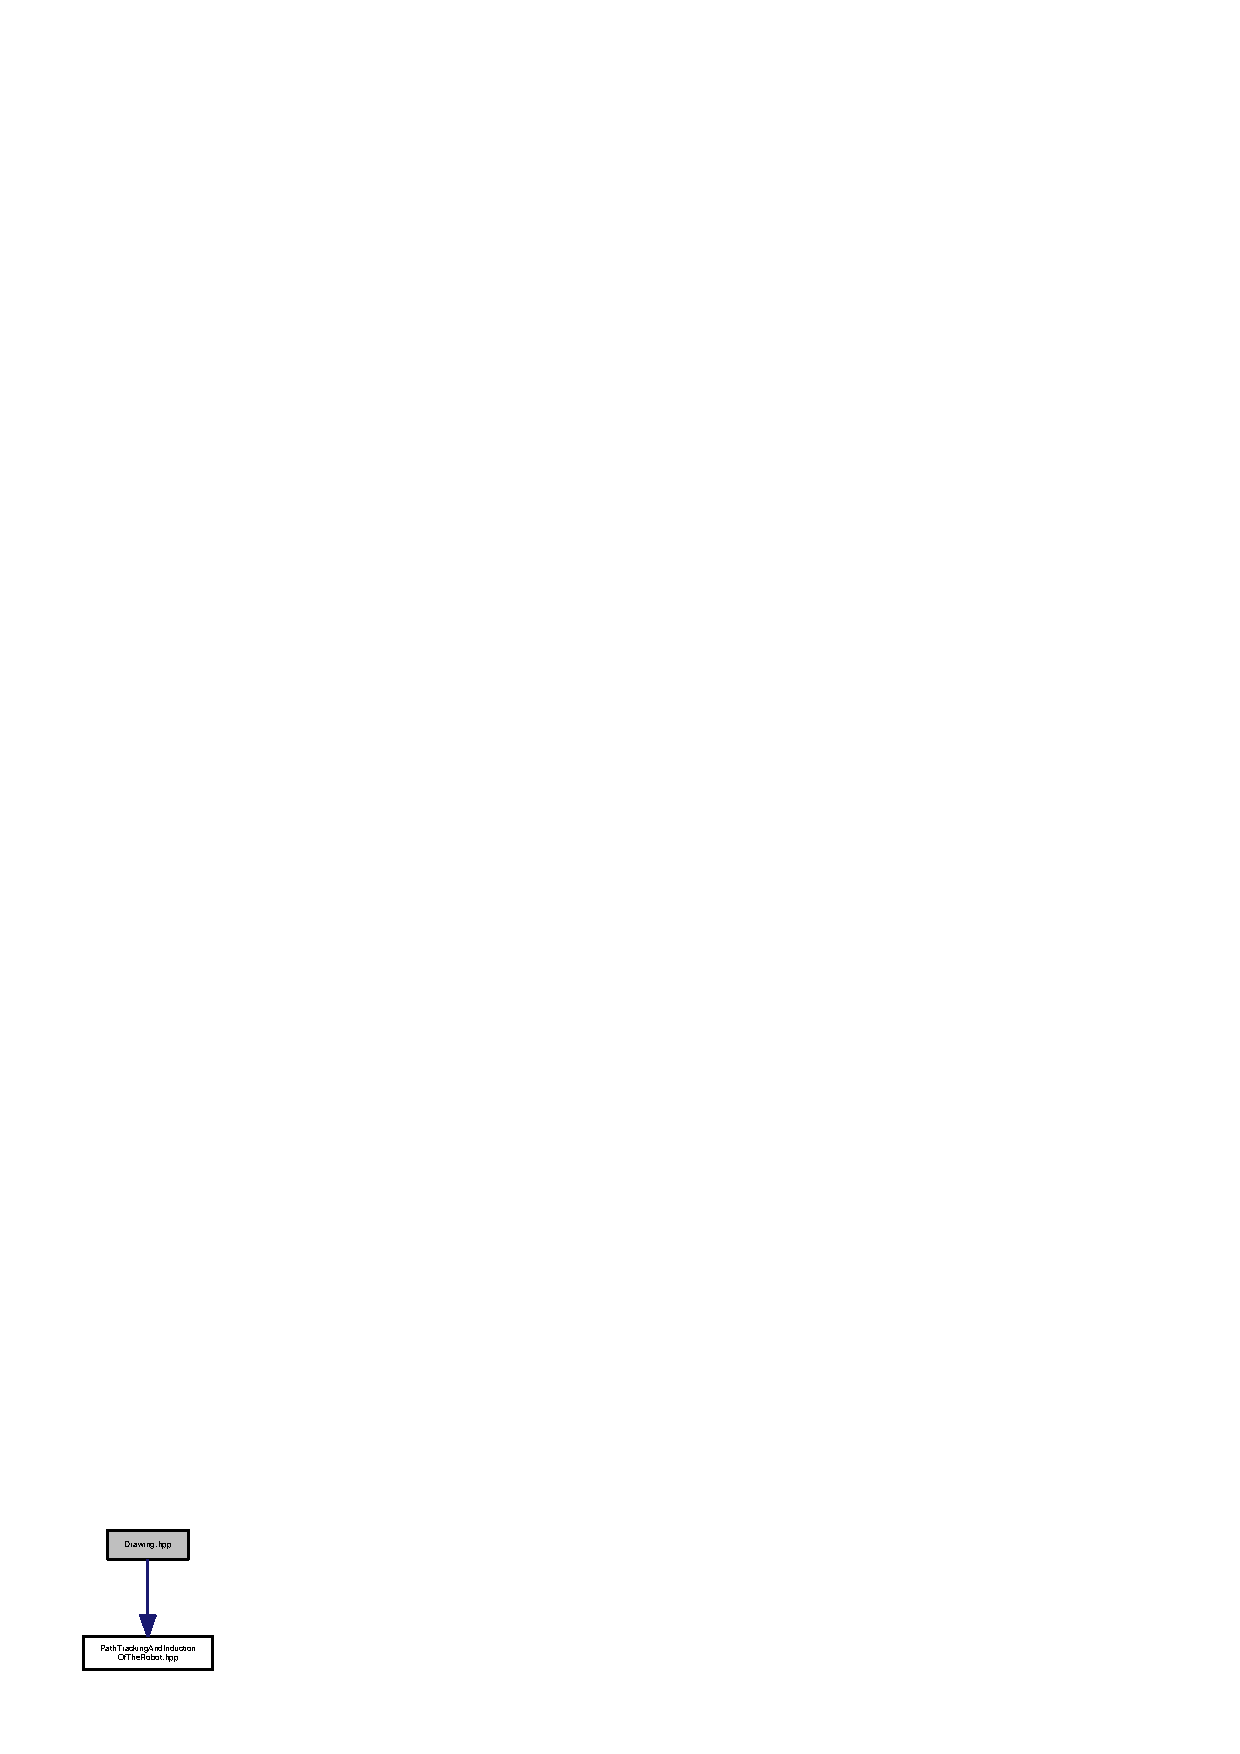
\includegraphics[width=106pt]{_drawing_8hpp__incl}
\end{center}
\end{figure}
被依存関係図\-:\nopagebreak
\begin{figure}[H]
\begin{center}
\leavevmode
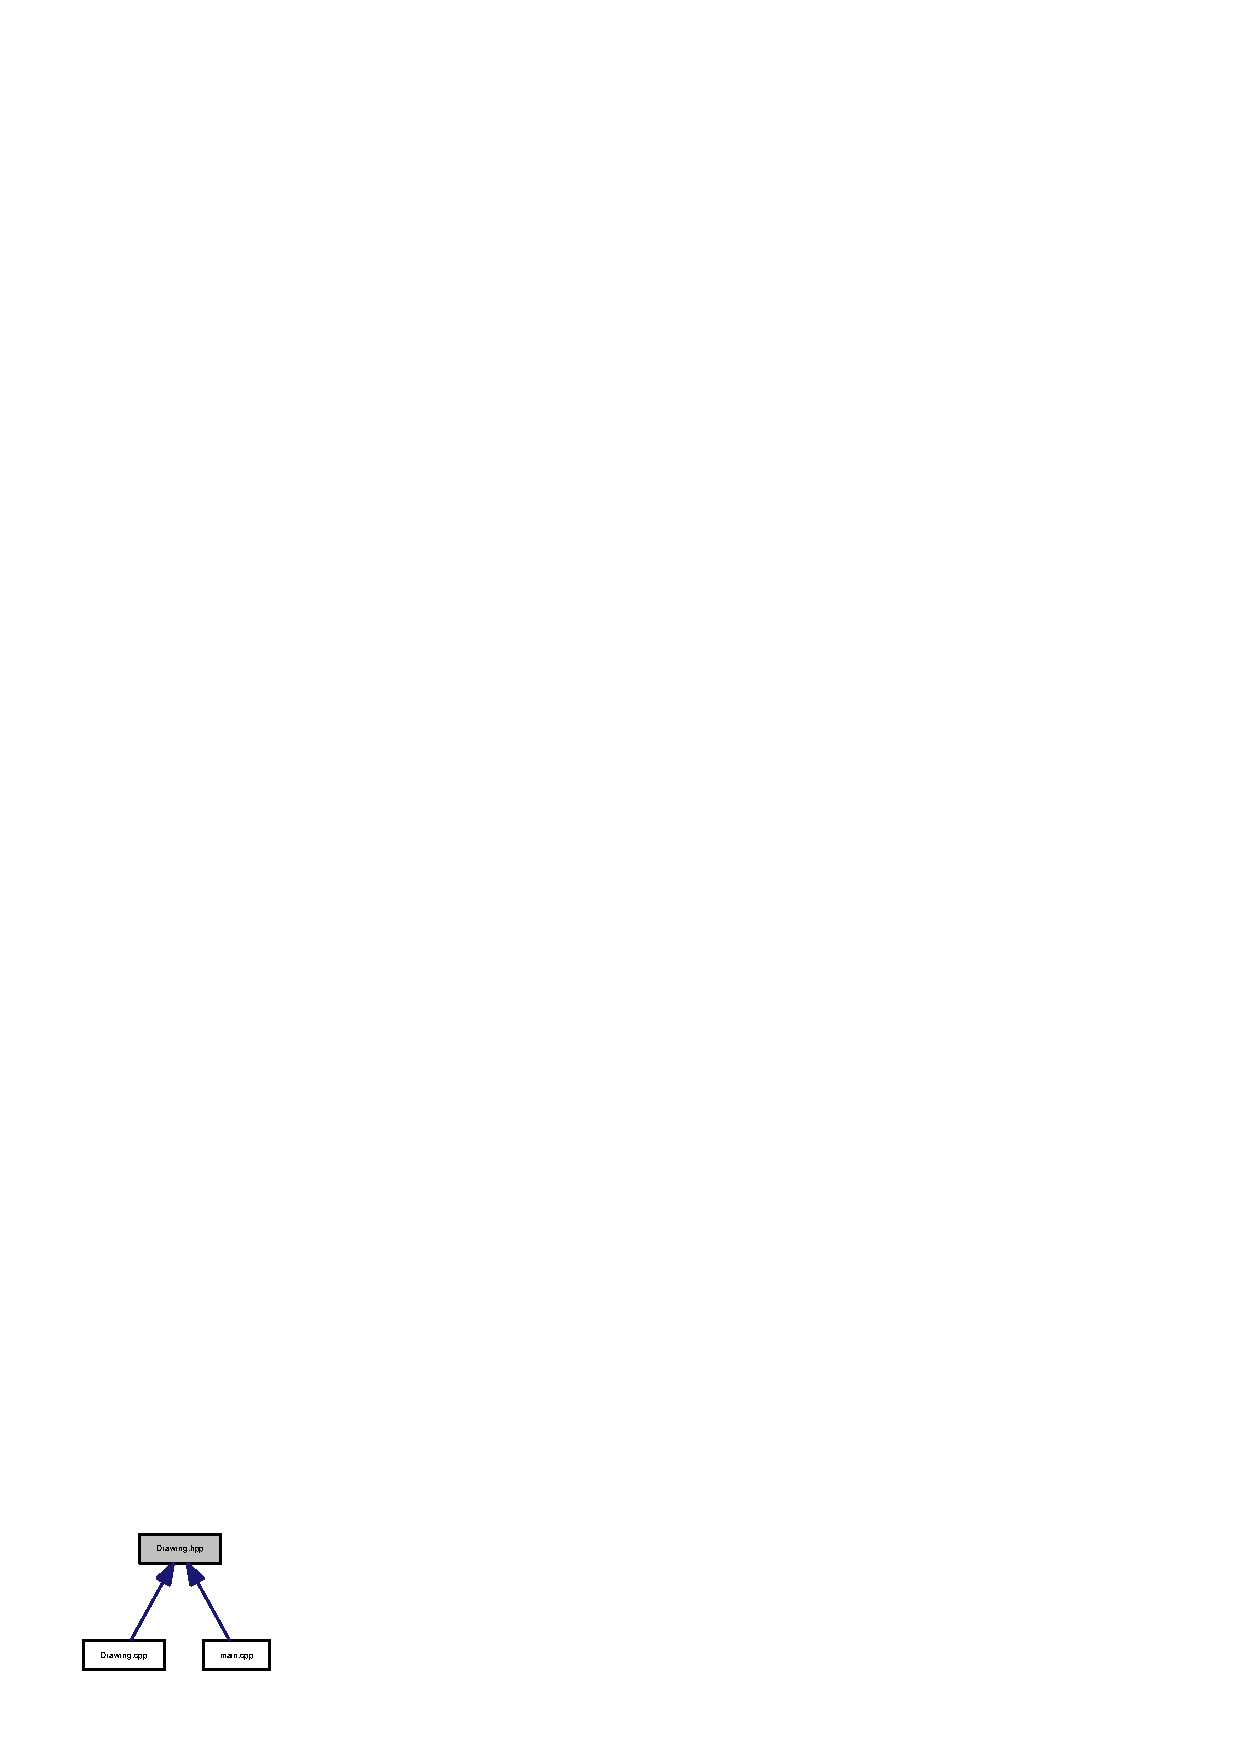
\includegraphics[width=134pt]{_drawing_8hpp__dep__incl}
\end{center}
\end{figure}
\subsection*{クラス}
\begin{DoxyCompactItemize}
\item 
class {\bf Drawing}
\begin{DoxyCompactList}\small\item\em 経路描画用のクラス \end{DoxyCompactList}\end{DoxyCompactItemize}

\section{E\-V3\-Control.\-cpp ファイル}
\label{_e_v3_control_8cpp}\index{E\-V3\-Control.\-cpp@{E\-V3\-Control.\-cpp}}
{\ttfamily \#include \char`\"{}Path\-Tracking\-And\-Induction\-Of\-The\-Robot.\-hpp\char`\"{}}\\*
{\ttfamily \#include \char`\"{}E\-V3\-Control.\-hpp\char`\"{}}\\*
E\-V3\-Control.\-cpp の依存先関係図\-:\nopagebreak
\begin{figure}[H]
\begin{center}
\leavevmode
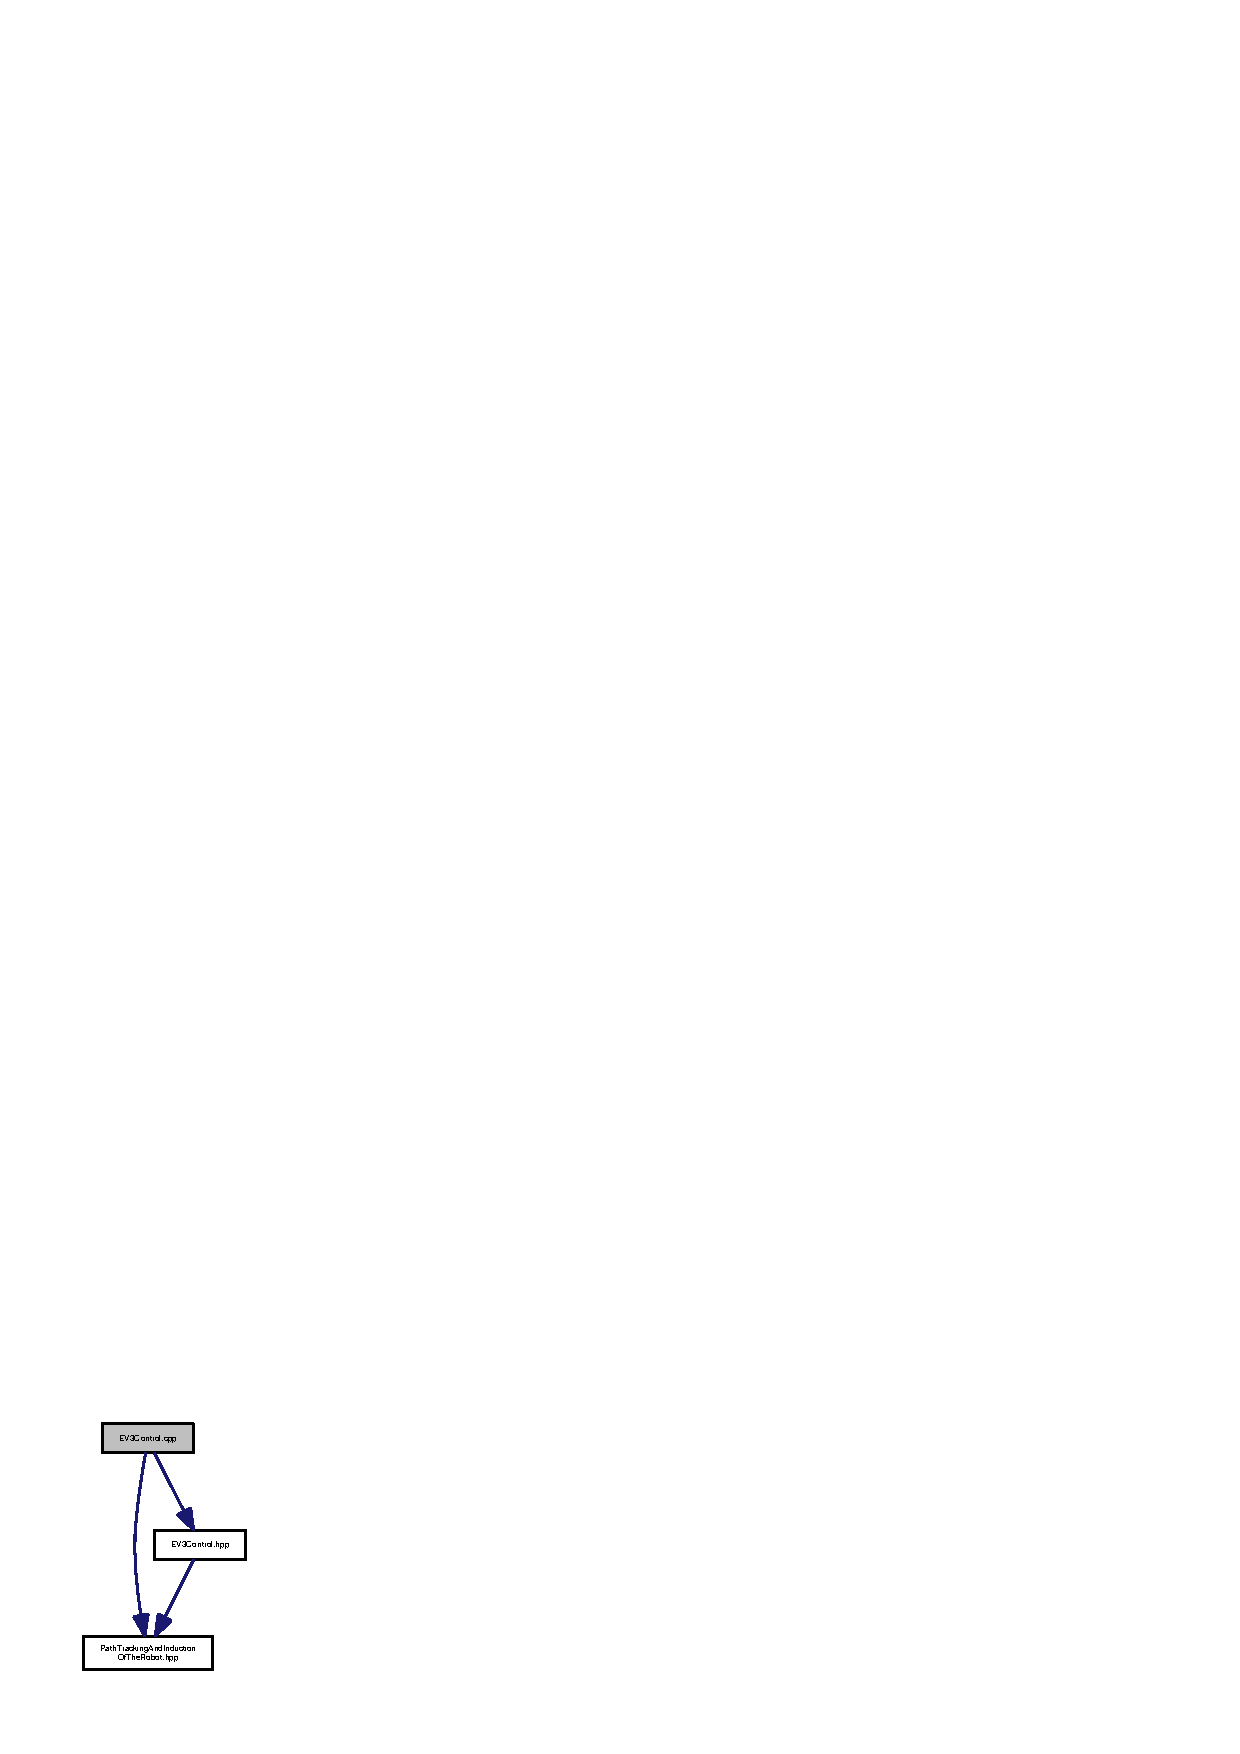
\includegraphics[width=122pt]{_e_v3_control_8cpp__incl}
\end{center}
\end{figure}

\section{E\-V3\-Control.\-hpp ファイル}
\label{_e_v3_control_8hpp}\index{E\-V3\-Control.\-hpp@{E\-V3\-Control.\-hpp}}
{\ttfamily \#include \char`\"{}Path\-Tracking\-And\-Induction\-Of\-The\-Robot.\-hpp\char`\"{}}\\*
E\-V3\-Control.\-hpp の依存先関係図\-:\nopagebreak
\begin{figure}[H]
\begin{center}
\leavevmode
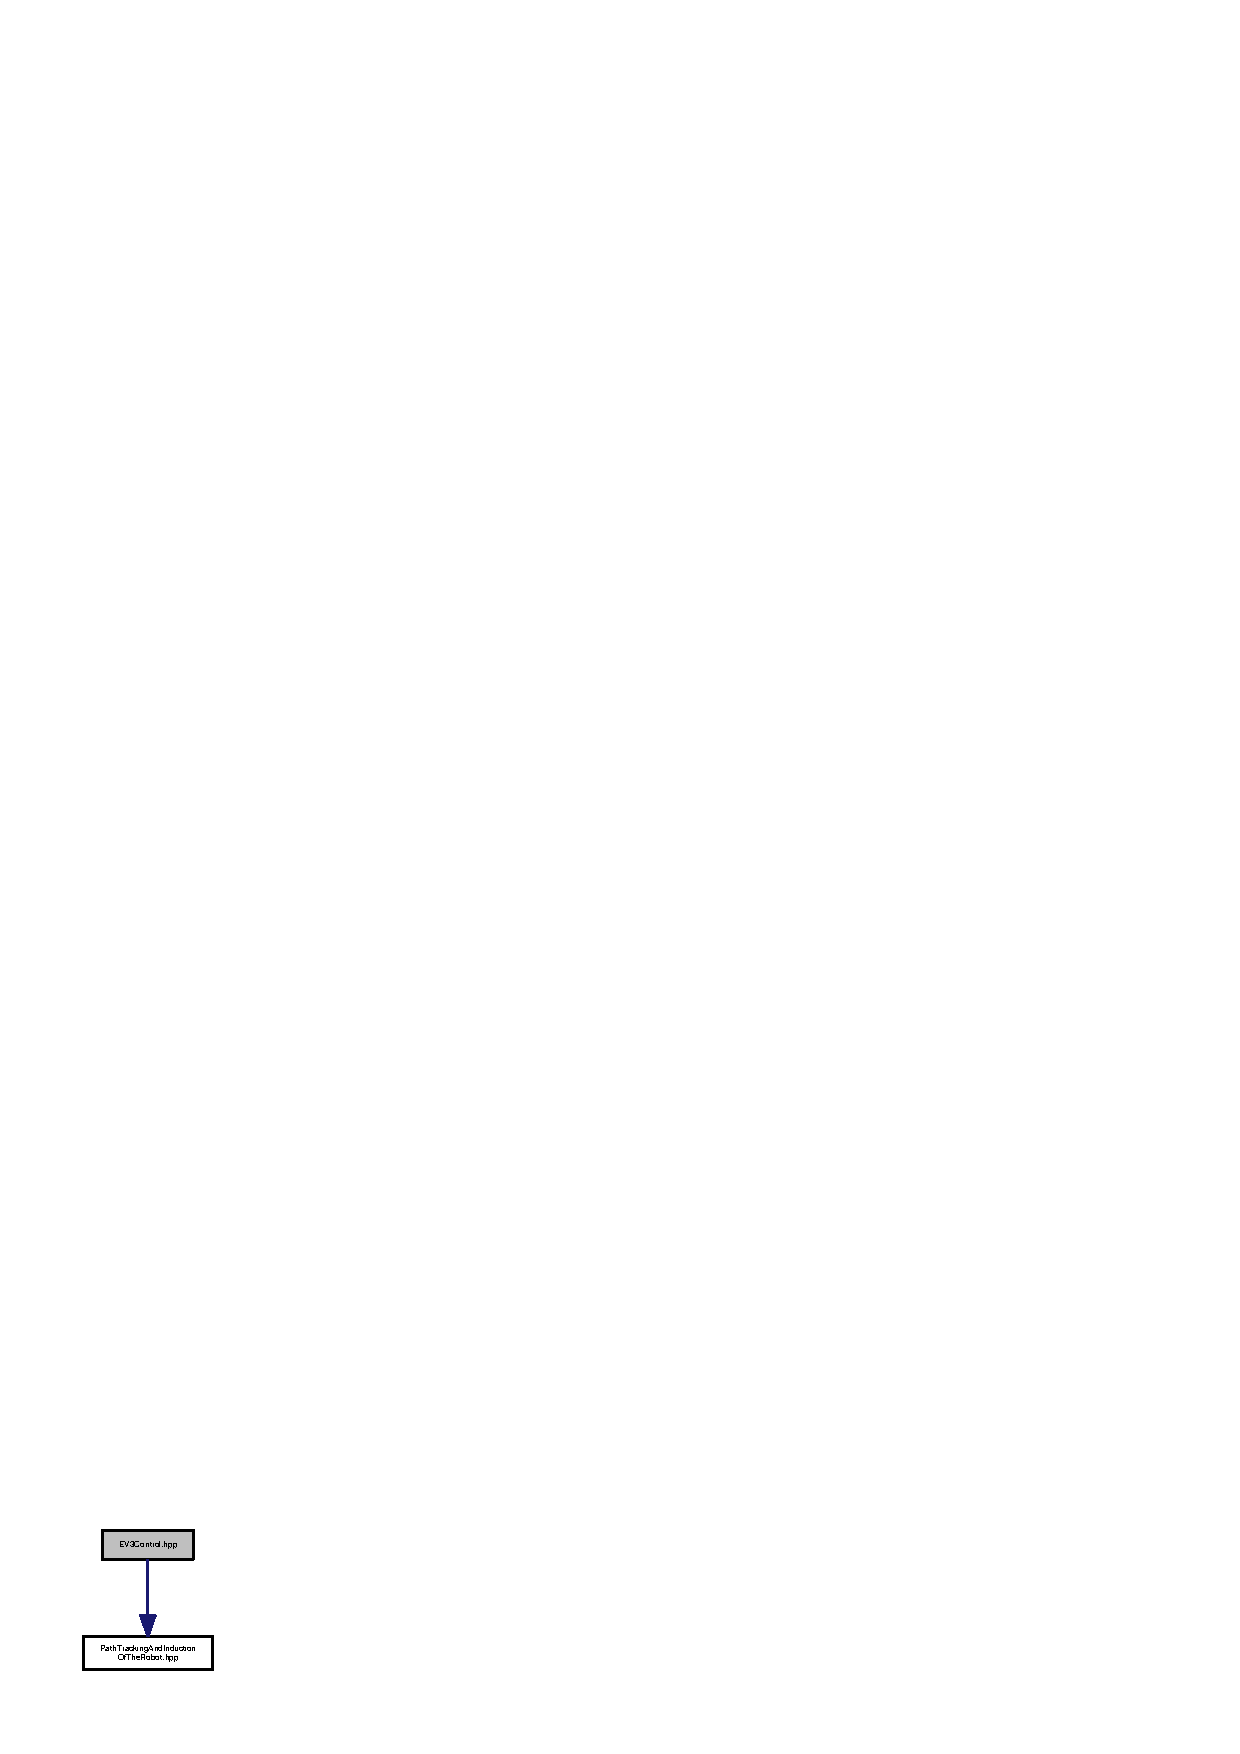
\includegraphics[width=106pt]{_e_v3_control_8hpp__incl}
\end{center}
\end{figure}
被依存関係図\-:\nopagebreak
\begin{figure}[H]
\begin{center}
\leavevmode
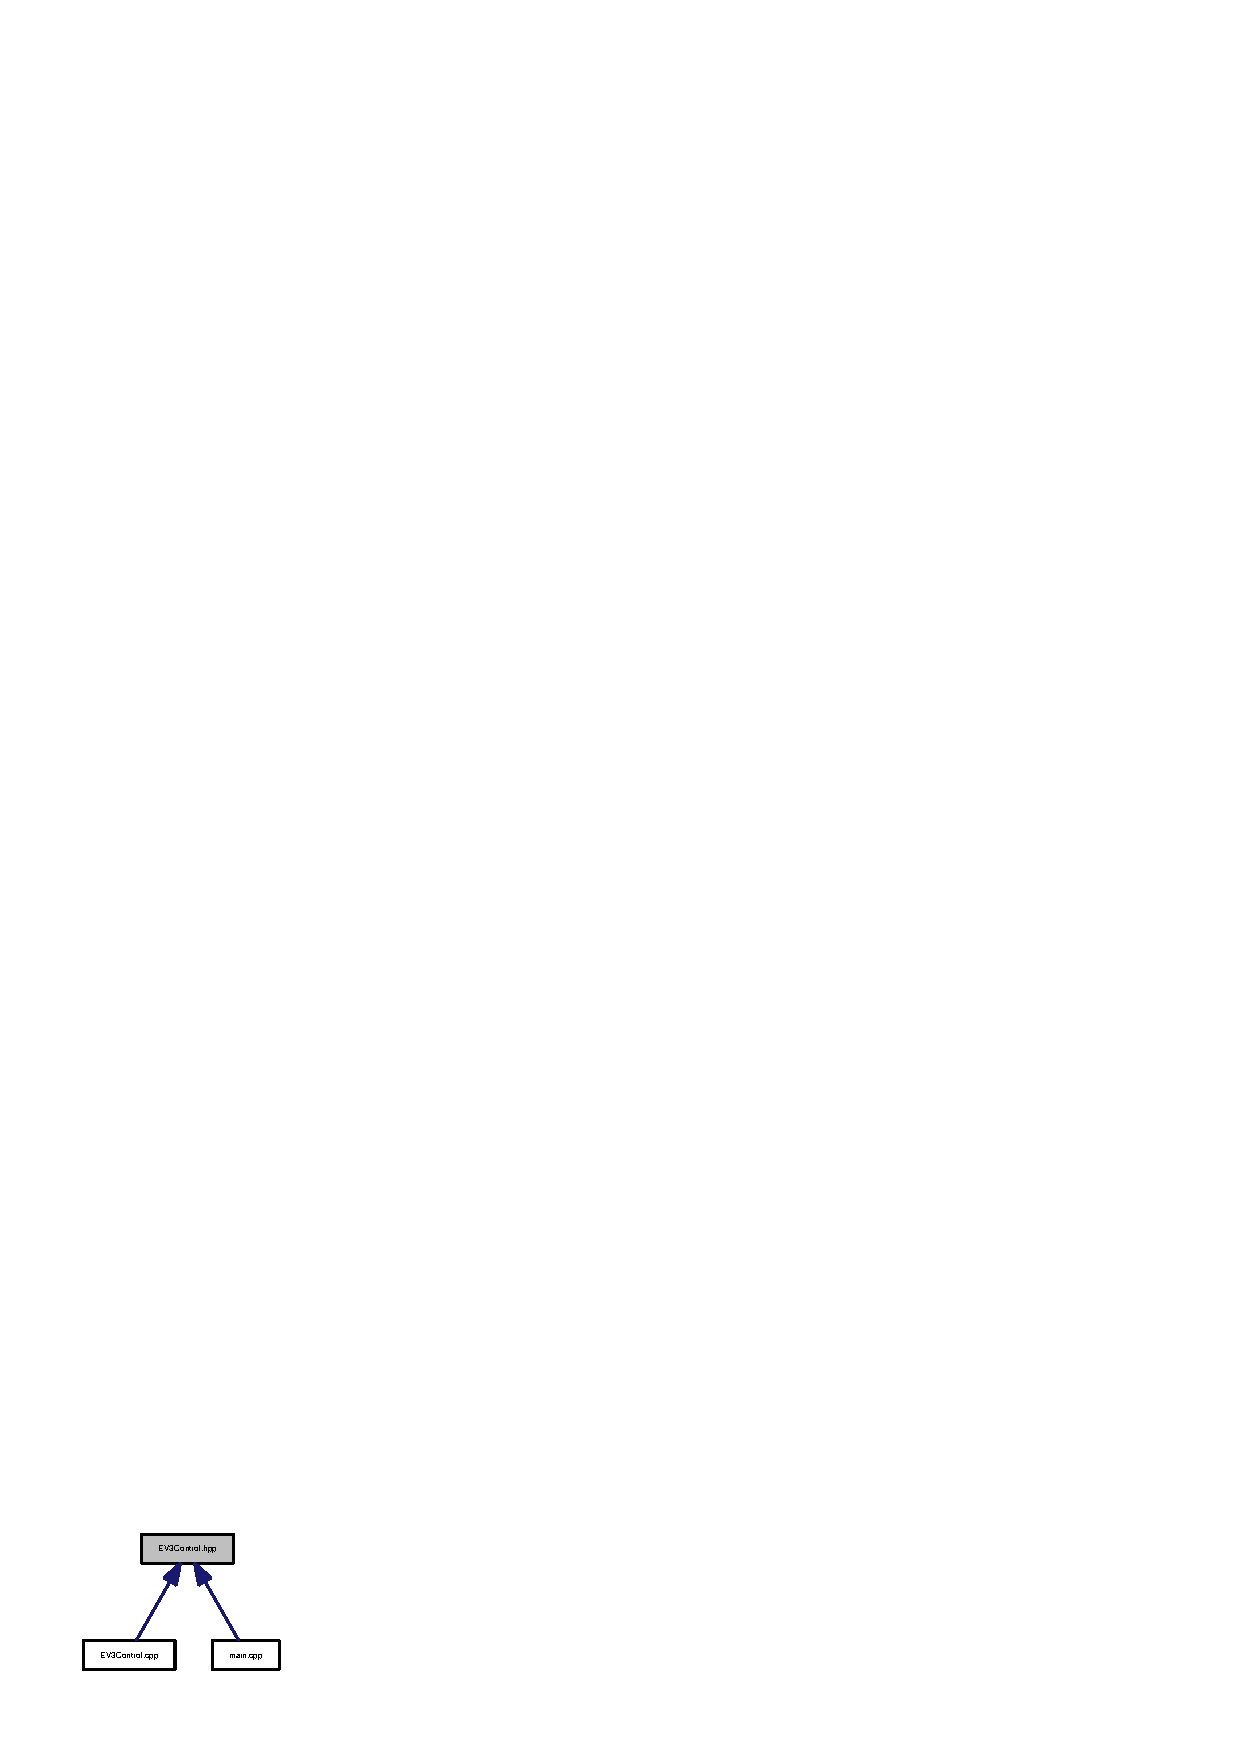
\includegraphics[width=138pt]{_e_v3_control_8hpp__dep__incl}
\end{center}
\end{figure}
\subsection*{クラス}
\begin{DoxyCompactItemize}
\item 
class {\bf E\-V3\-Control}
\begin{DoxyCompactList}\small\item\em E\-V3を制御するためのクラス \end{DoxyCompactList}\end{DoxyCompactItemize}

\section{Image\-Processing.\-cpp ファイル}
\label{_image_processing_8cpp}\index{Image\-Processing.\-cpp@{Image\-Processing.\-cpp}}
{\ttfamily \#include \char`\"{}Path\-Tracking\-And\-Induction\-Of\-The\-Robot.\-hpp\char`\"{}}\\*
{\ttfamily \#include \char`\"{}Image\-Processing.\-hpp\char`\"{}}\\*
Image\-Processing.\-cpp の依存先関係図\-:\nopagebreak
\begin{figure}[H]
\begin{center}
\leavevmode
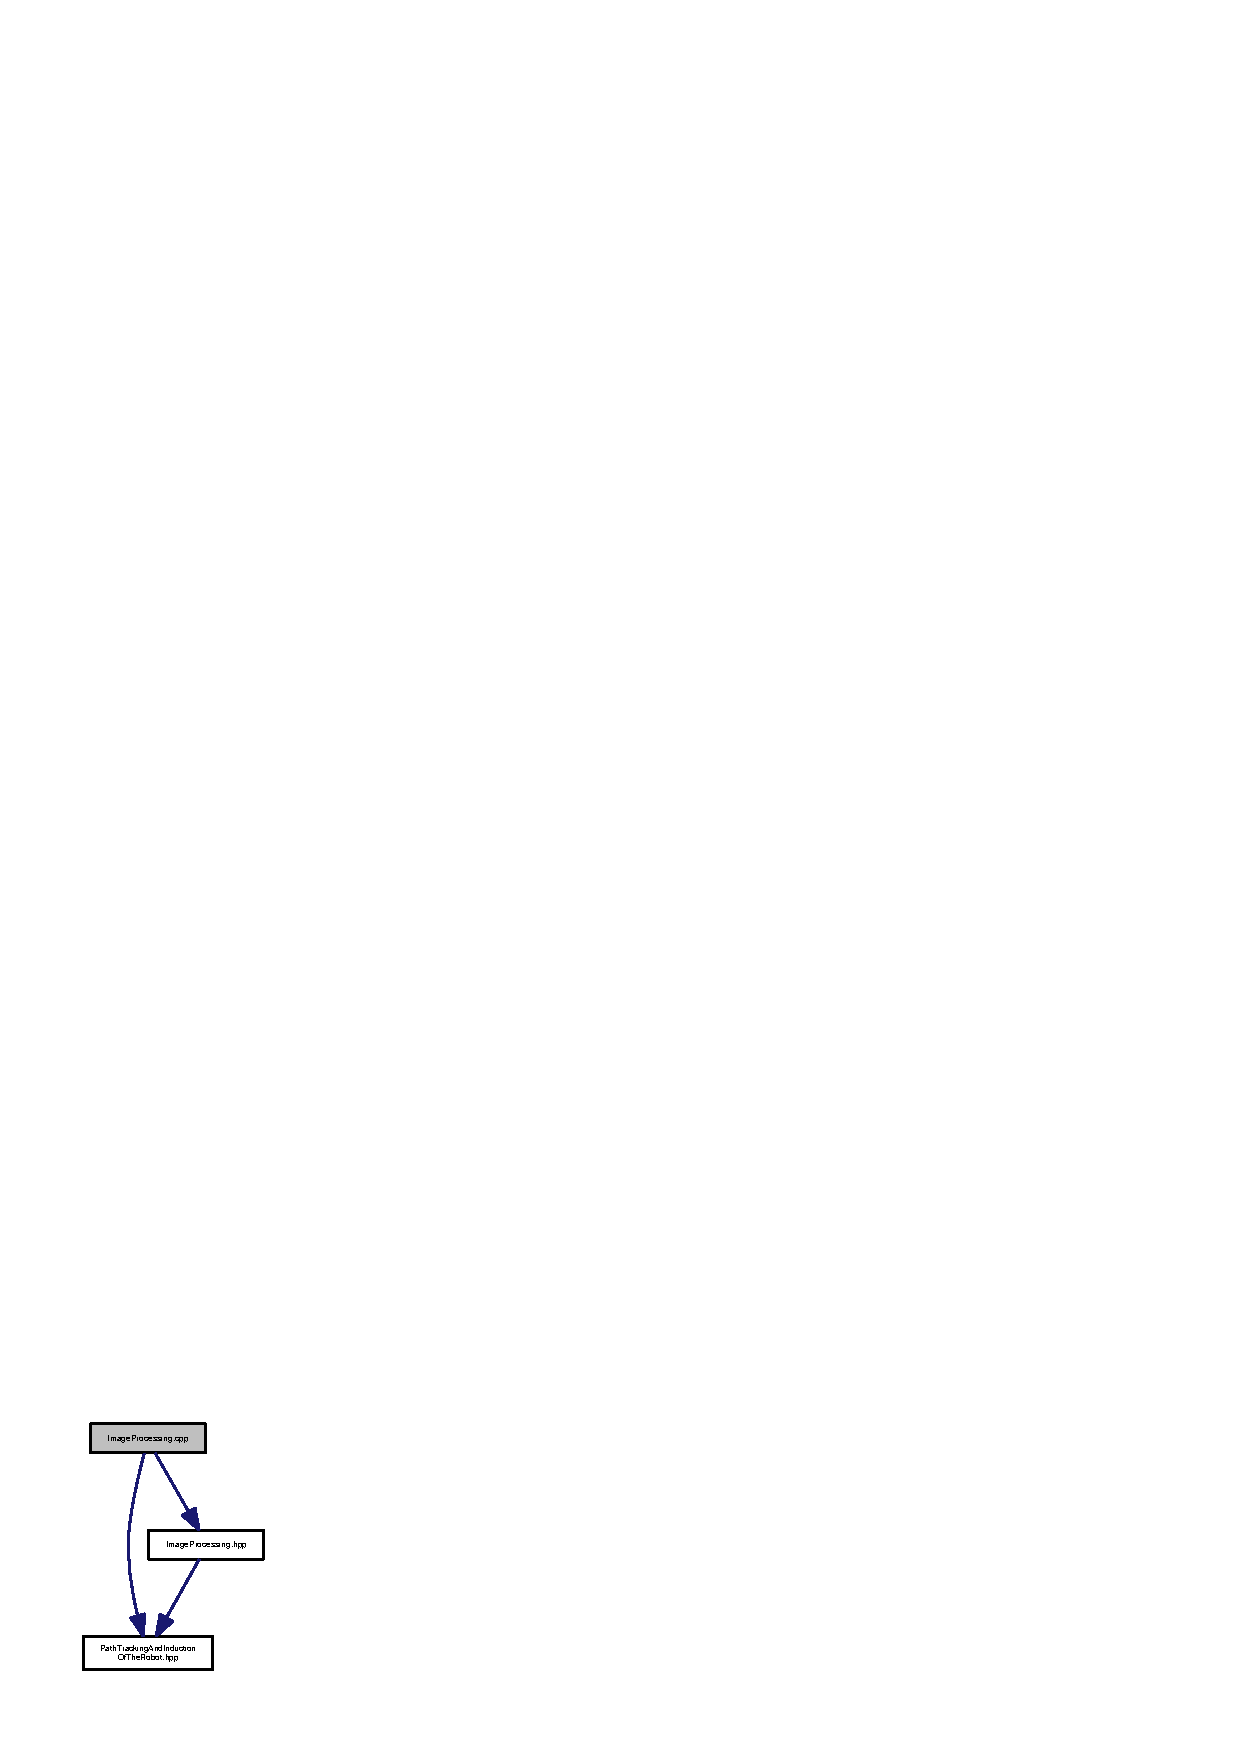
\includegraphics[width=131pt]{_image_processing_8cpp__incl}
\end{center}
\end{figure}

\section{Image\-Processing.\-hpp ファイル}
\label{_image_processing_8hpp}\index{Image\-Processing.\-hpp@{Image\-Processing.\-hpp}}
{\ttfamily \#include \char`\"{}Path\-Tracking\-And\-Induction\-Of\-The\-Robot.\-hpp\char`\"{}}\\*
\subsection*{クラス}
\begin{DoxyCompactItemize}
\item 
class {\bf Image\-Processing}
\begin{DoxyCompactList}\small\item\em 画像処理用のクラス \end{DoxyCompactList}\end{DoxyCompactItemize}

\section{Kinect.\-cpp ファイル}
\label{_kinect_8cpp}\index{Kinect.\-cpp@{Kinect.\-cpp}}
{\ttfamily \#include \char`\"{}Path\-Tracking\-And\-Induction\-Of\-The\-Robot.\-hpp\char`\"{}}\\*
{\ttfamily \#include \char`\"{}Kinect.\-hpp\char`\"{}}\\*

\section{Kinect.\-hpp ファイル}
\label{_kinect_8hpp}\index{Kinect.\-hpp@{Kinect.\-hpp}}
{\ttfamily \#include \char`\"{}Path\-Tracking\-And\-Induction\-Of\-The\-Robot.\-hpp\char`\"{}}\\*
\subsection*{クラス}
\begin{DoxyCompactItemize}
\item 
class {\bf Kinect}
\begin{DoxyCompactList}\small\item\em Kinect操作用のクラス \end{DoxyCompactList}\end{DoxyCompactItemize}
\subsection*{マクロ定義}
\begin{DoxyCompactItemize}
\item 
\#define {\bf E\-R\-R\-O\-R\-\_\-\-C\-H\-E\-C\-K}(ret)
\begin{DoxyCompactList}\small\item\em エラーチェック \end{DoxyCompactList}\end{DoxyCompactItemize}
\subsection*{変数}
\begin{DoxyCompactItemize}
\item 
const N\-U\-I\-\_\-\-I\-M\-A\-G\-E\-\_\-\-R\-E\-S\-O\-L\-U\-T\-I\-O\-N {\bf C\-A\-M\-E\-R\-A\-\_\-\-R\-E\-S\-O\-L\-U\-T\-I\-O\-N} = N\-U\-I\-\_\-\-I\-M\-A\-G\-E\-\_\-\-R\-E\-S\-O\-L\-U\-T\-I\-O\-N\-\_\-640x480
\end{DoxyCompactItemize}


\subsection{マクロ定義詳解}
\index{Kinect.\-hpp@{Kinect.\-hpp}!E\-R\-R\-O\-R\-\_\-\-C\-H\-E\-C\-K@{E\-R\-R\-O\-R\-\_\-\-C\-H\-E\-C\-K}}
\index{E\-R\-R\-O\-R\-\_\-\-C\-H\-E\-C\-K@{E\-R\-R\-O\-R\-\_\-\-C\-H\-E\-C\-K}!Kinect.hpp@{Kinect.\-hpp}}
\subsubsection[{E\-R\-R\-O\-R\-\_\-\-C\-H\-E\-C\-K}]{\setlength{\rightskip}{0pt plus 5cm}\#define E\-R\-R\-O\-R\-\_\-\-C\-H\-E\-C\-K(
\begin{DoxyParamCaption}
\item[{}]{ret}
\end{DoxyParamCaption}
)}\label{_kinect_8hpp_a60155ea06e80f9ce19fbf58d043f3287}
{\bfseries 値\-:}
\begin{DoxyCode}
\textcolor{keywordflow}{if} (ret != S\_OK)\{ \(\backslash\)
stringstream ss; \(\backslash\)
ss << \textcolor{stringliteral}{"faild"} #ret \textcolor{stringliteral}{" "} << hex << ret << endl; \(\backslash\)
throw runtime\_error(ss.str().c\_str()); \(\backslash\)
\}
\end{DoxyCode}


エラーチェック 



 Kinect.\-hpp の 17 行目に定義があります。



参照元 Kinect\-::create\-Instance(), Kinect\-::draw\-R\-G\-B\-Image(), Kinect\-::get\-Point\-Cloud(), Kinect\-::initialize().



\subsection{変数詳解}
\index{Kinect.\-hpp@{Kinect.\-hpp}!C\-A\-M\-E\-R\-A\-\_\-\-R\-E\-S\-O\-L\-U\-T\-I\-O\-N@{C\-A\-M\-E\-R\-A\-\_\-\-R\-E\-S\-O\-L\-U\-T\-I\-O\-N}}
\index{C\-A\-M\-E\-R\-A\-\_\-\-R\-E\-S\-O\-L\-U\-T\-I\-O\-N@{C\-A\-M\-E\-R\-A\-\_\-\-R\-E\-S\-O\-L\-U\-T\-I\-O\-N}!Kinect.hpp@{Kinect.\-hpp}}
\subsubsection[{C\-A\-M\-E\-R\-A\-\_\-\-R\-E\-S\-O\-L\-U\-T\-I\-O\-N}]{\setlength{\rightskip}{0pt plus 5cm}const N\-U\-I\-\_\-\-I\-M\-A\-G\-E\-\_\-\-R\-E\-S\-O\-L\-U\-T\-I\-O\-N C\-A\-M\-E\-R\-A\-\_\-\-R\-E\-S\-O\-L\-U\-T\-I\-O\-N = N\-U\-I\-\_\-\-I\-M\-A\-G\-E\-\_\-\-R\-E\-S\-O\-L\-U\-T\-I\-O\-N\-\_\-640x480}\label{_kinect_8hpp_ac0e005483bfce51f732e38048c0b1898}
Kinectの解像度の設定 

 Kinect.\-hpp の 25 行目に定義があります。



参照元 Kinect\-::get\-Point\-Cloud(), Kinect\-::initialize().


\section{Least\-Square\-Method.\-cpp ファイル}
\label{_least_square_method_8cpp}\index{Least\-Square\-Method.\-cpp@{Least\-Square\-Method.\-cpp}}
{\ttfamily \#include \char`\"{}Path\-Tracking\-And\-Induction\-Of\-The\-Robot.\-hpp\char`\"{}}\\*
{\ttfamily \#include \char`\"{}Least\-Square\-Method.\-hpp\char`\"{}}\\*
Least\-Square\-Method.\-cpp の依存先関係図\-:\nopagebreak
\begin{figure}[H]
\begin{center}
\leavevmode
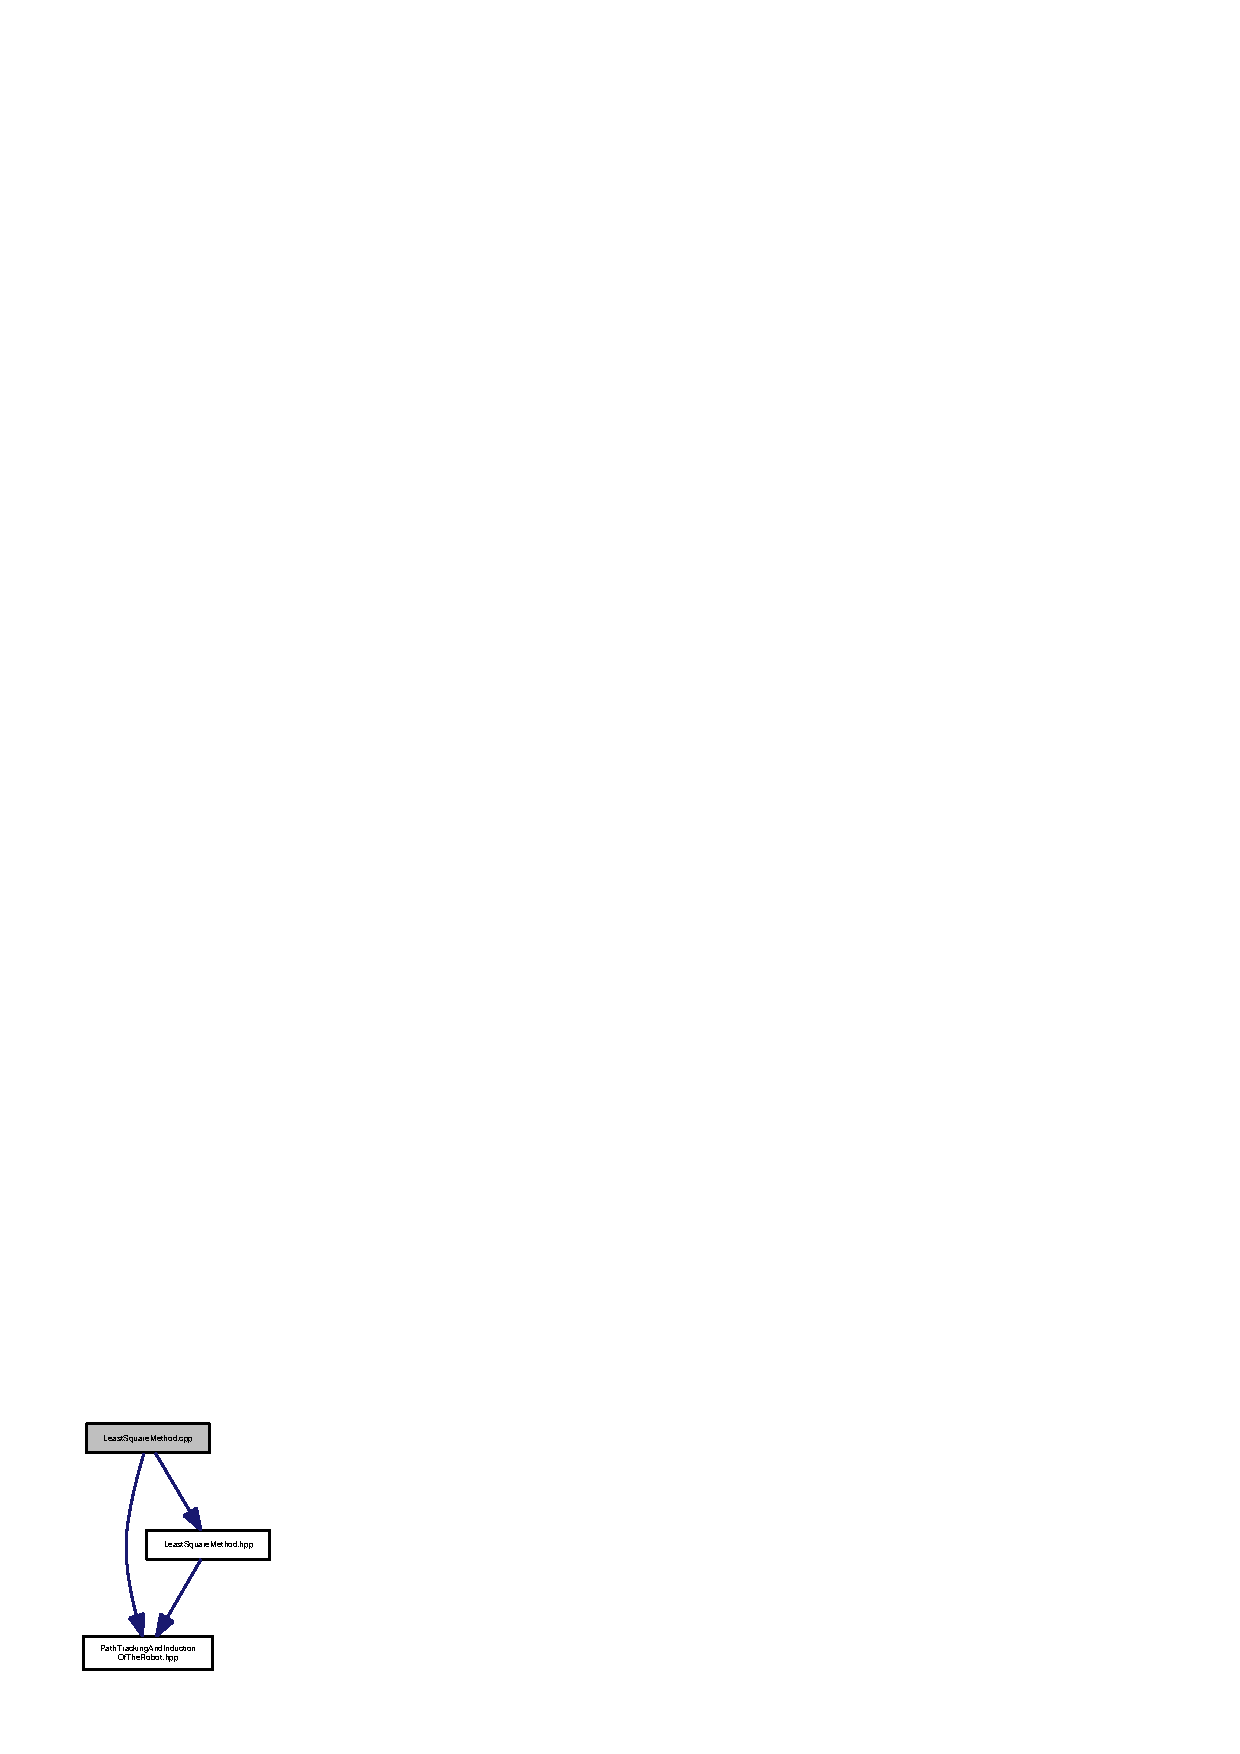
\includegraphics[width=134pt]{_least_square_method_8cpp__incl}
\end{center}
\end{figure}

\section{Least\-Square\-Method.\-hpp ファイル}
\label{_least_square_method_8hpp}\index{Least\-Square\-Method.\-hpp@{Least\-Square\-Method.\-hpp}}
{\ttfamily \#include \char`\"{}Path\-Tracking\-And\-Induction\-Of\-The\-Robot.\-hpp\char`\"{}}\\*
Least\-Square\-Method.\-hpp の依存先関係図\-:\nopagebreak
\begin{figure}[H]
\begin{center}
\leavevmode
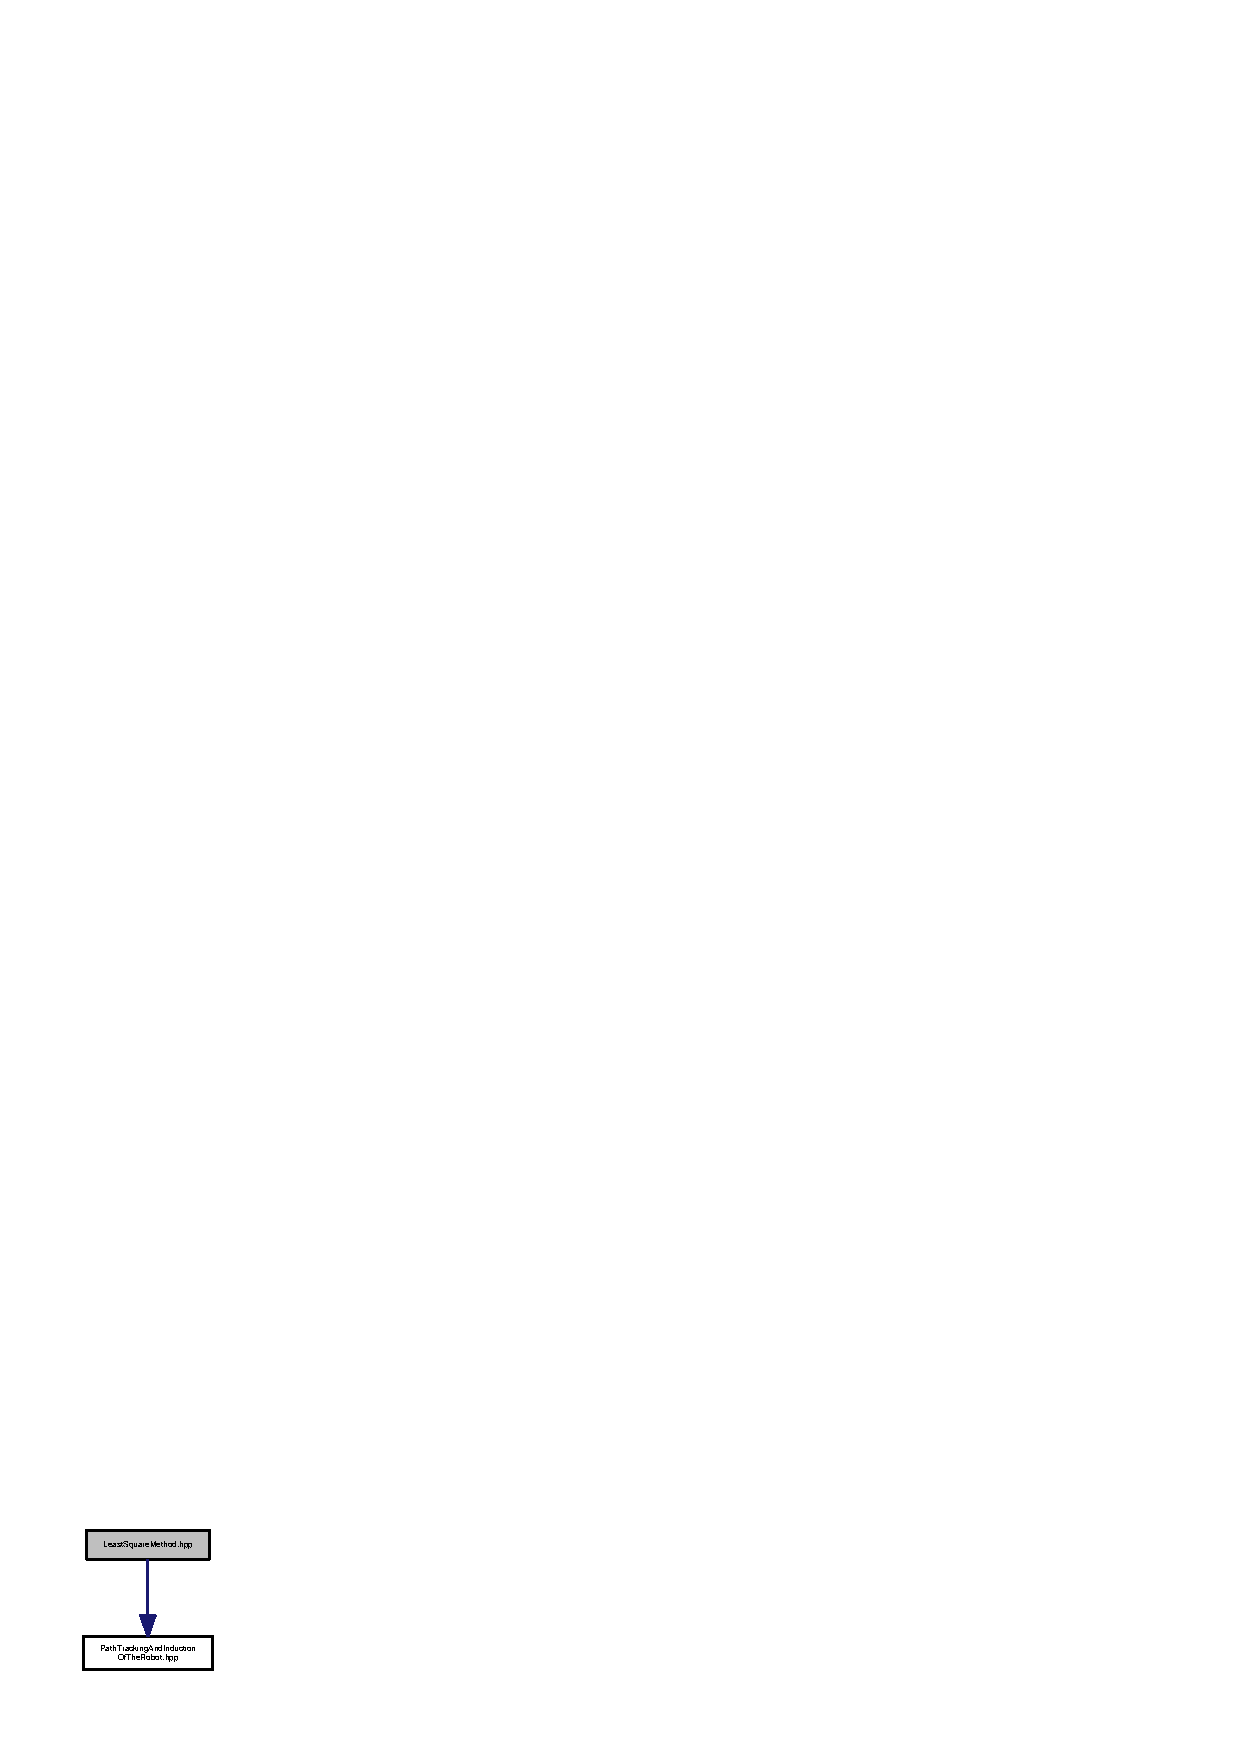
\includegraphics[width=106pt]{_least_square_method_8hpp__incl}
\end{center}
\end{figure}
被依存関係図\-:\nopagebreak
\begin{figure}[H]
\begin{center}
\leavevmode
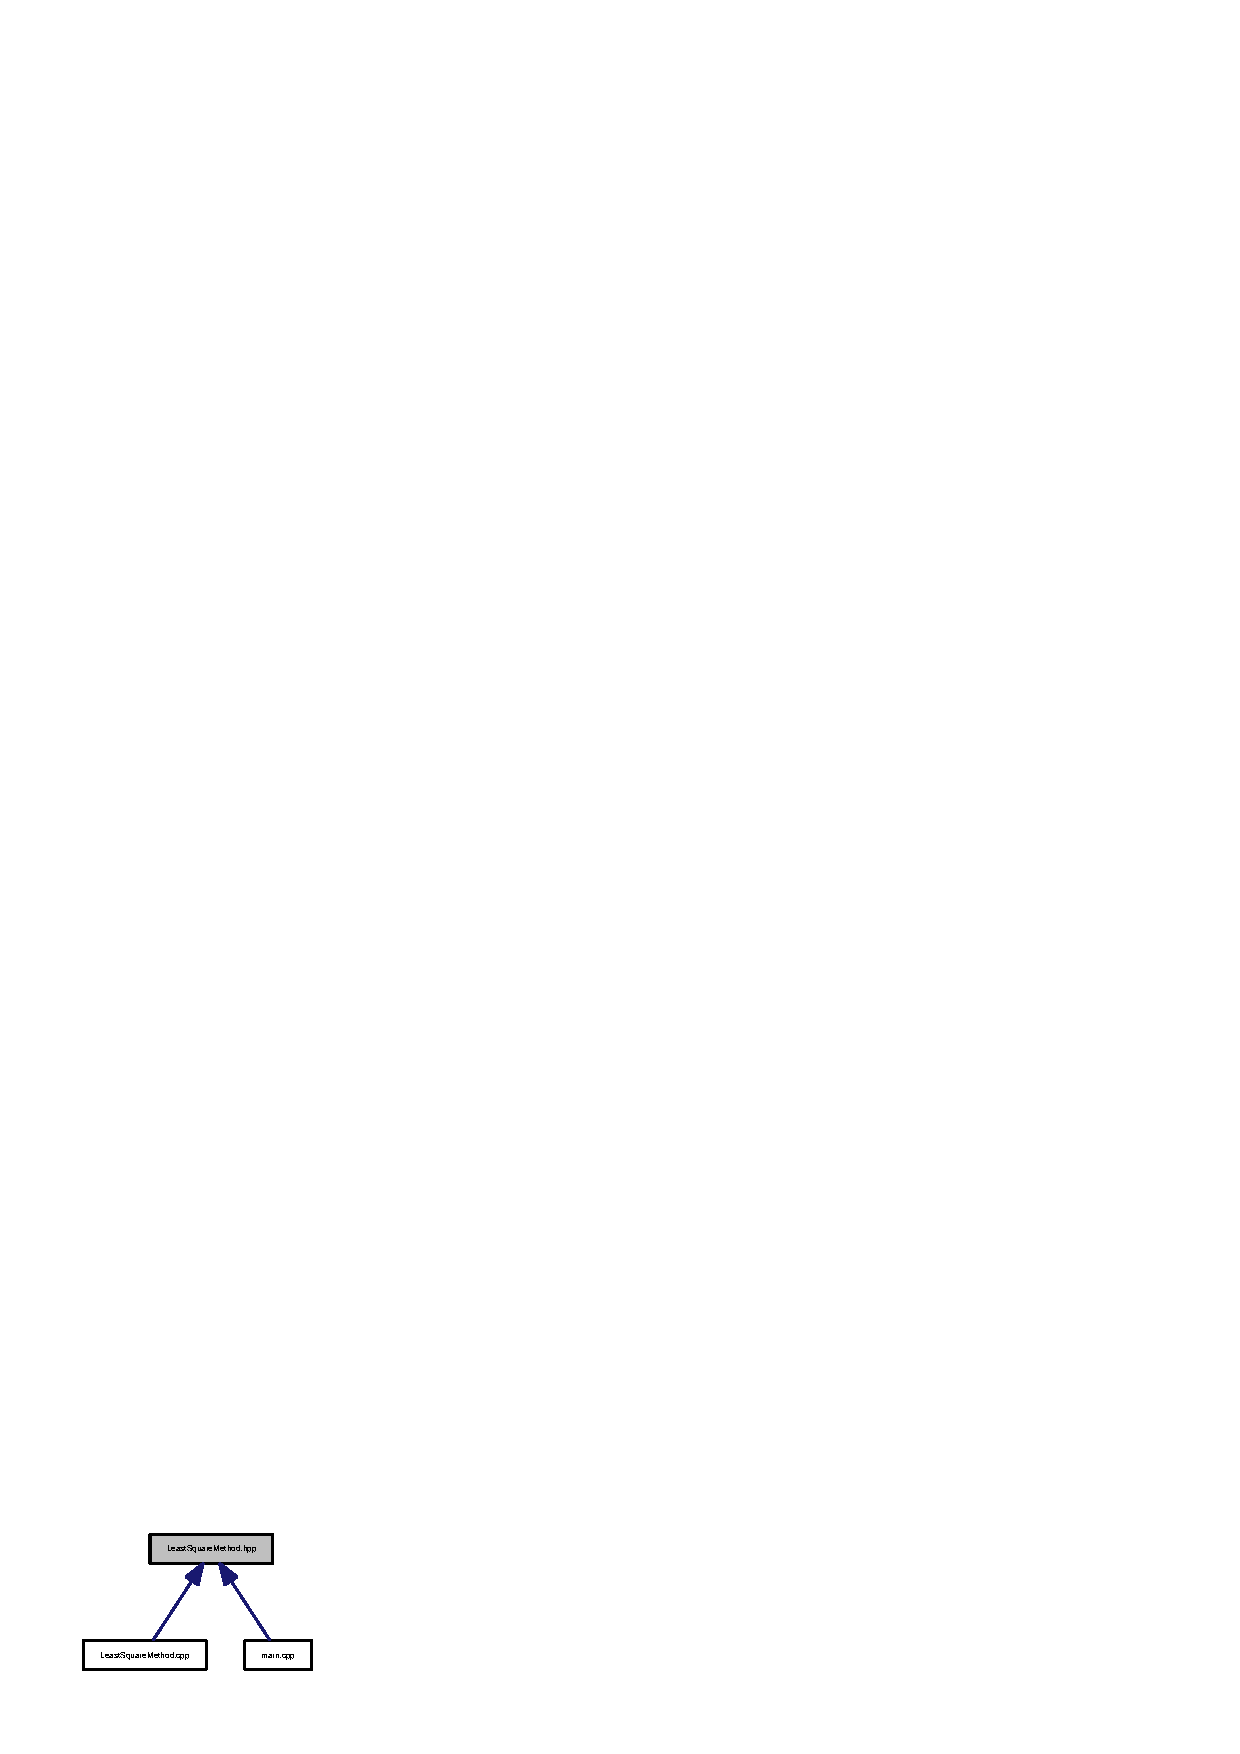
\includegraphics[width=154pt]{_least_square_method_8hpp__dep__incl}
\end{center}
\end{figure}
\subsection*{クラス}
\begin{DoxyCompactItemize}
\item 
class {\bf Least\-Square\-Method}
\begin{DoxyCompactList}\small\item\em 最小二乗法を行うクラス \end{DoxyCompactList}\end{DoxyCompactItemize}

\section{main.\-cpp ファイル}
\label{main_8cpp}\index{main.\-cpp@{main.\-cpp}}
{\ttfamily \#include \char`\"{}Path\-Tracking\-And\-Induction\-Of\-The\-Robot.\-hpp\char`\"{}}\\*
{\ttfamily \#include \char`\"{}Kinect.\-hpp\char`\"{}}\\*
{\ttfamily \#include \char`\"{}Image\-Processing.\-hpp\char`\"{}}\\*
{\ttfamily \#include \char`\"{}Drawing.\-hpp\char`\"{}}\\*
{\ttfamily \#include \char`\"{}System.\-hpp\char`\"{}}\\*
{\ttfamily \#include \char`\"{}Least\-Square\-Method.\-hpp\char`\"{}}\\*
{\ttfamily \#include \char`\"{}Point\-Cloud\-Library.\-hpp\char`\"{}}\\*
{\ttfamily \#include \char`\"{}E\-V3\-Control.\-hpp\char`\"{}}\\*
main.\-cpp の依存先関係図\-:\nopagebreak
\begin{figure}[H]
\begin{center}
\leavevmode
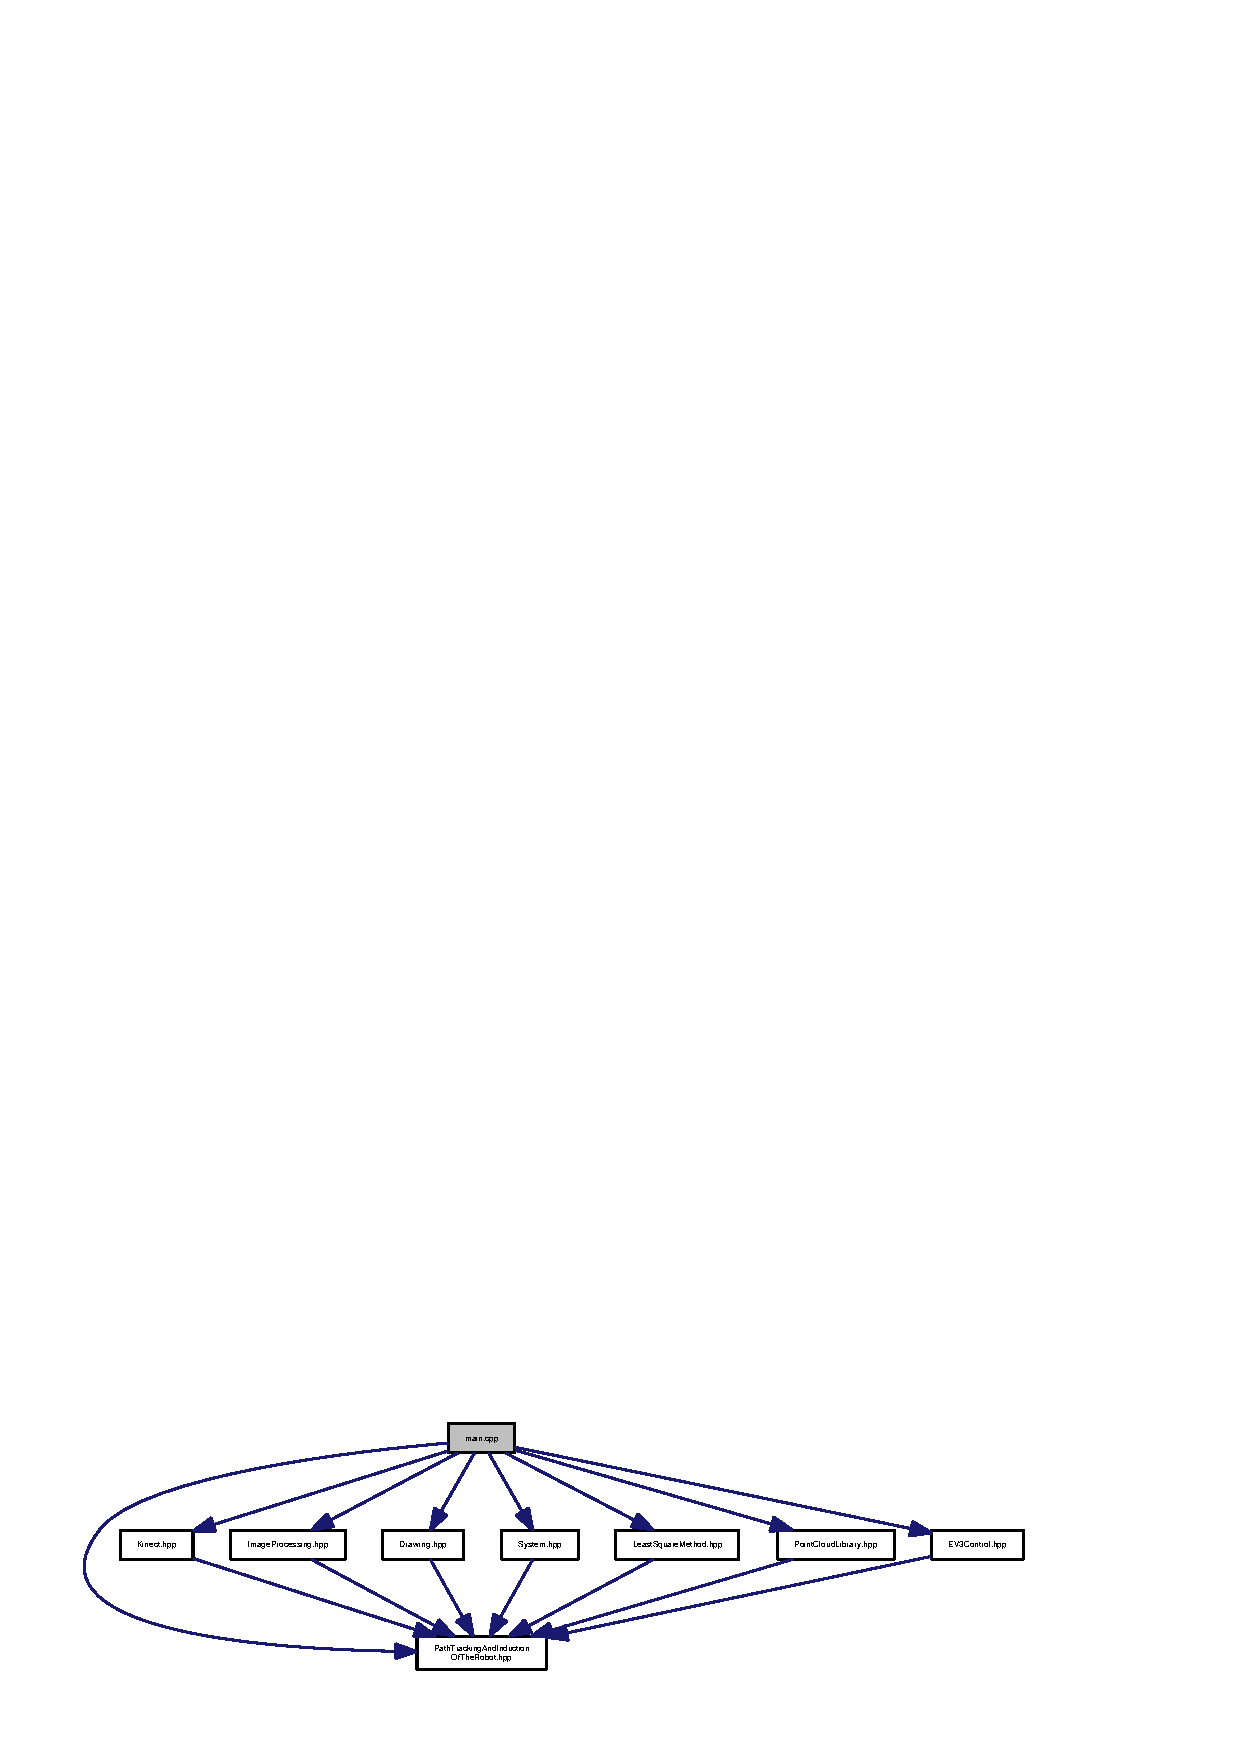
\includegraphics[width=350pt]{main_8cpp__incl}
\end{center}
\end{figure}
\subsection*{関数}
\begin{DoxyCompactItemize}
\item 
void {\bf on\-Mouse} (int event, int x, int y, int flags, void $\ast$param)
\begin{DoxyCompactList}\small\item\em マウス操作 \end{DoxyCompactList}\item 
int {\bf main} ()
\begin{DoxyCompactList}\small\item\em 関数main() \end{DoxyCompactList}\end{DoxyCompactItemize}
\subsection*{変数}
\begin{DoxyCompactItemize}
\item 
Mat {\bf image}
\begin{DoxyCompactList}\small\item\em R\-G\-B画像格納用の変数 \end{DoxyCompactList}\item 
char {\bf directory\-Name} [{\bf N\-O\-C}]
\begin{DoxyCompactList}\small\item\em フォルダ名 \end{DoxyCompactList}\item 
bool {\bf select\-Object} = false
\begin{DoxyCompactList}\small\item\em オブジェクト選択 \end{DoxyCompactList}\item 
int {\bf track\-Object} = 0
\begin{DoxyCompactList}\small\item\em 追跡するオブジェクト \end{DoxyCompactList}\item 
Point {\bf origin}
\begin{DoxyCompactList}\small\item\em オリジナルの座標 \end{DoxyCompactList}\item 
Rect {\bf selection}
\begin{DoxyCompactList}\small\item\em 選択 \end{DoxyCompactList}\end{DoxyCompactItemize}


\subsection{関数詳解}
\index{main.\-cpp@{main.\-cpp}!main@{main}}
\index{main@{main}!main.cpp@{main.\-cpp}}
\subsubsection[{main}]{\setlength{\rightskip}{0pt plus 5cm}int main (
\begin{DoxyParamCaption}
{}
\end{DoxyParamCaption}
)}\label{main_8cpp_ae66f6b31b5ad750f1fe042a706a4e3d4}


関数main() 

\begin{DoxyReturn}{戻り値}
0 正常終了 

-\/1 異常終了 
\end{DoxyReturn}
pointcloudlibrary.\-viewer-\/$>$was\-Stopped() \&\&

$<$平均座標を確認するための球 

 main.\-cpp の 36 行目に定義があります。



参照先 System\-::alternatives(), Least\-Square\-Method\-::attitude\-\_\-angle, Least\-Square\-Method\-::calc\-Yaw\-Roll\-Pitch(), Point\-Cloud\-Library\-::centroid, System\-::check\-Directory(), Least\-Square\-Method\-::coefficient\-\_\-plane, System\-::countdown\-Timer(), directory\-Name, Point\-Cloud\-Library\-::downsampling\-\_\-flag, Point\-Cloud\-Library\-::down\-Sampling\-Using\-Voxel\-Grid\-Filter(), Kinect\-::draw\-R\-G\-B\-Image(), System\-::end\-Message(), System\-::end\-Timer(), Point\-Cloud\-Library\-::extractplane\-\_\-flag, Point\-Cloud\-Library\-::flag\-Checker(), E\-V3\-Control\-::get\-Average\-Velocity\-And\-Yaw(), Image\-Processing\-::get\-Background\-Substraction\-Bin\-Image(), Point\-Cloud\-Library\-::get\-Centroid\-Coordinate3d(), Least\-Square\-Method\-::get\-Coefficient(), Point\-Cloud\-Library\-::get\-Extract\-Plane\-And\-Clustering(), System\-::get\-Frame\-Rate(), Kinect\-::get\-Point\-Cloud(), System\-::get\-Process\-Timein\-Miliseconds(), Image\-Processing\-::get\-Undistortion\-Image(), E\-V3\-Control\-::get\-Velocityin\-Sec(), Drawing\-::gnuplot\-Script\-E\-V3(), Drawing\-::gnuplot\-Script\-E\-V3\-Route(), Drawing\-::gnuplot\-Script\-Time2\-V(), Drawing\-::gnuplot\-Script\-Time2\-Yaw(), image, Kinect\-::initialize(), Point\-Cloud\-Library\-::initialize\-P\-C\-L\-Visualizer(), Kinect\-::key, Image\-Processing\-::load\-Internal\-Camera\-Parameter(), System\-::make\-Directory(), System\-::make\-Directory\-Based\-Date(), Point\-Cloud\-Library\-::mls\-\_\-flag, N\-O\-C, Image\-Processing\-::open\-C\-V\-Setting\-Trackbar(), E\-V3\-Control\-::output6\-Do\-F(), E\-V3\-Control\-::output6\-Do\-F\-Continuous(), E\-V3\-Control\-::output\-Control\-Information(), E\-V3\-Control\-::output\-E\-V3\-Route\-Continuous(), Image\-Processing\-::output\-Image\-Select\-Directory(), Point\-Cloud\-Library\-::output\-Point\-Cloud(), Point\-Cloud\-Library\-::output\-Point\-Cloud\-P\-L\-Y(), Point\-Cloud\-Library\-::passthrough\-\_\-flag, Point\-Cloud\-Library\-::pass\-Through\-Filter(), System\-::remove\-Directory(), Point\-Cloud\-Library\-::remove\-Outlier(), E\-V3\-Control\-::save\-\_\-flag, E\-V3\-Control\-::set6\-Do\-F\-E\-V3(), System\-::show\-Help\-Message(), Image\-Processing\-::show\-Image(), Point\-Cloud\-Library\-::smoothing\-Using\-Moving\-Least\-Square(), System\-::start\-Message(), System\-::start\-Timer(), Point\-Cloud\-Library\-::statisticaloutlierremoval\-\_\-flag, Kinect\-::stream\-Event, System\-::sum\-\_\-time, Point\-Cloud\-Library\-::visualizer (計61項目).



呼び出し関係図\-:\nopagebreak
\begin{figure}[H]
\begin{center}
\leavevmode
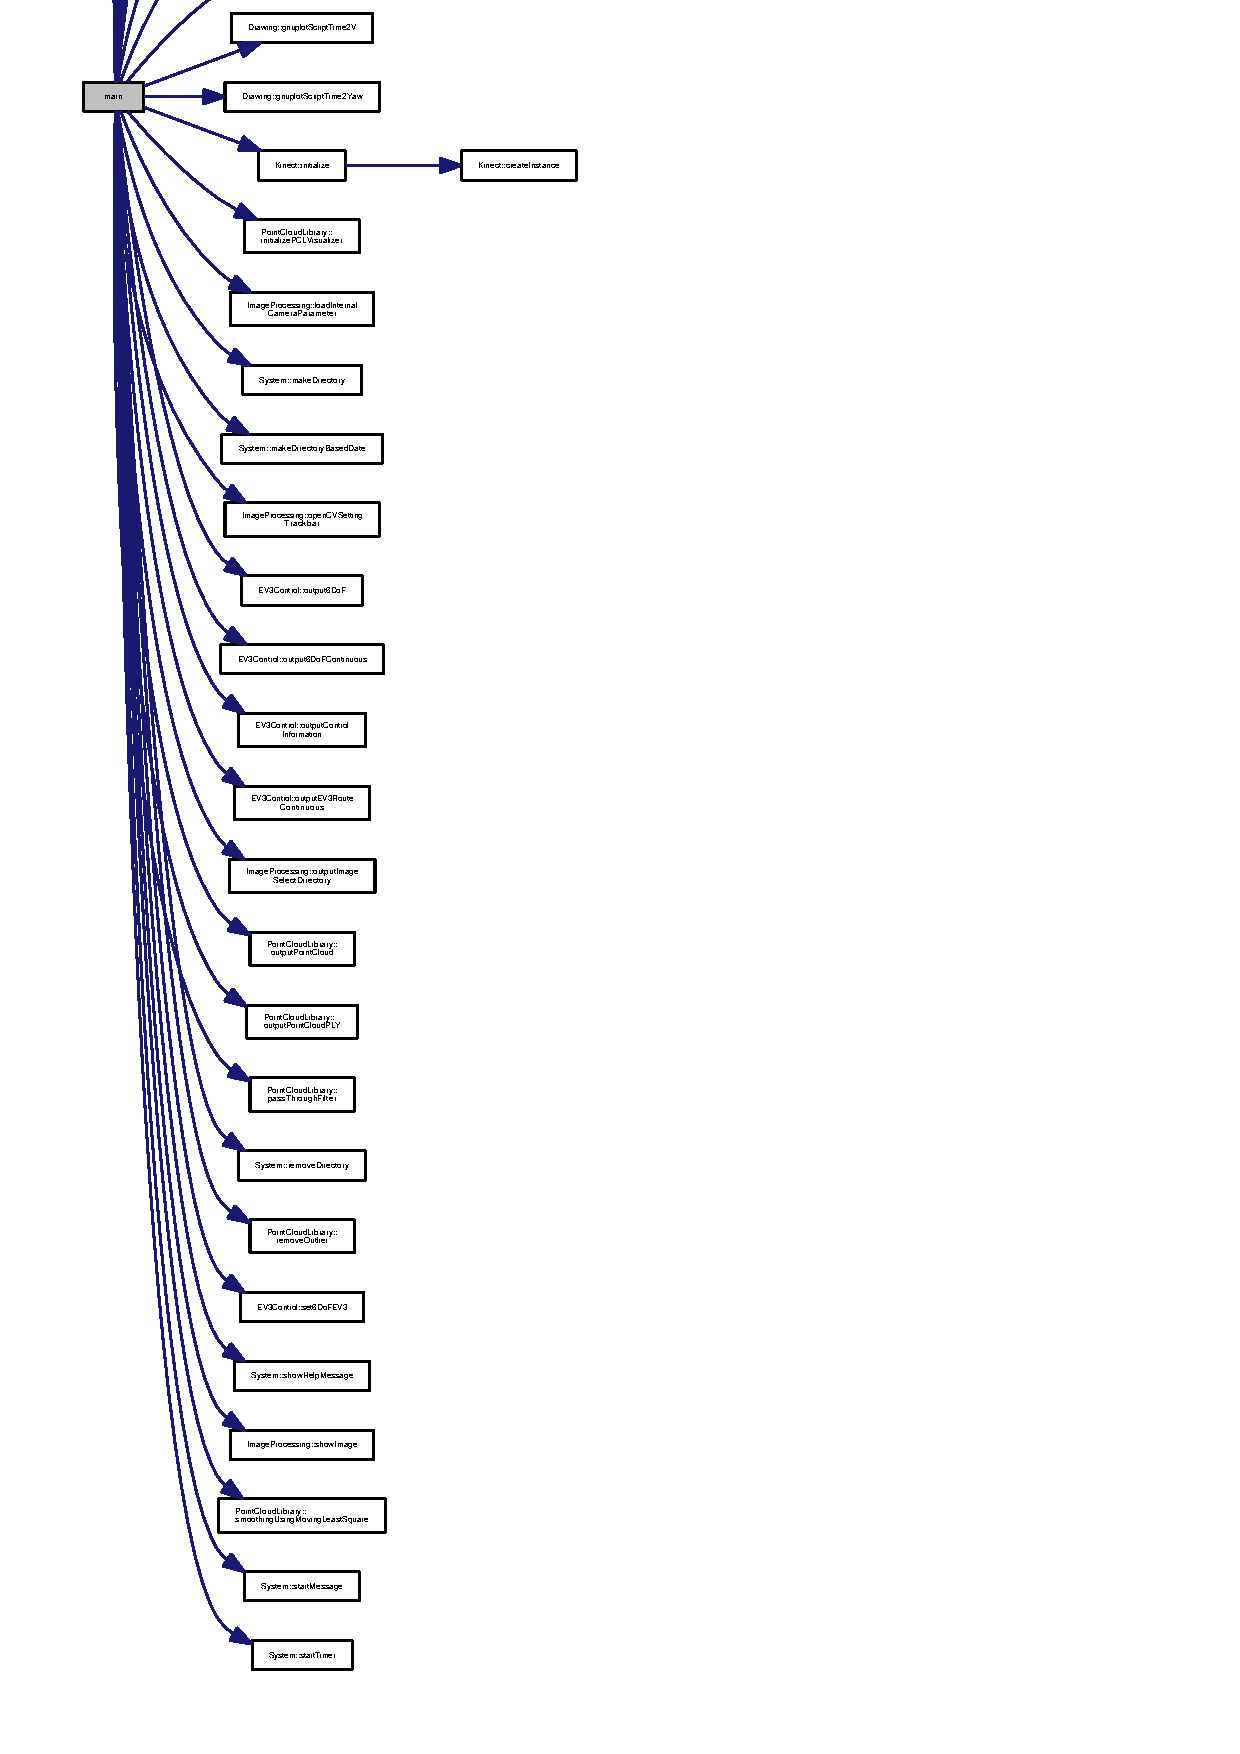
\includegraphics[height=550pt]{main_8cpp_ae66f6b31b5ad750f1fe042a706a4e3d4_cgraph}
\end{center}
\end{figure}


\index{main.\-cpp@{main.\-cpp}!on\-Mouse@{on\-Mouse}}
\index{on\-Mouse@{on\-Mouse}!main.cpp@{main.\-cpp}}
\subsubsection[{on\-Mouse}]{\setlength{\rightskip}{0pt plus 5cm}void on\-Mouse (
\begin{DoxyParamCaption}
\item[{int}]{event, }
\item[{int}]{x, }
\item[{int}]{y, }
\item[{int}]{flags, }
\item[{void $\ast$}]{param}
\end{DoxyParamCaption}
)}\label{main_8cpp_ab6ccc6c8d80970d4178c943533533860}


マウス操作 

マウス操作


\begin{DoxyParams}{引数}
{\em event} & int 型.イベント \\
\hline
{\em x} & int型.x座標 \\
\hline
{\em y} & int型.y座標 \\
\hline
{\em flags} & int型.フラグ \\
\hline
{\em param} & void$\ast$型.その他パラメータ \\
\hline
\end{DoxyParams}


 Mouse.\-cpp の 19 行目に定義があります。



\subsection{変数詳解}
\index{main.\-cpp@{main.\-cpp}!directory\-Name@{directory\-Name}}
\index{directory\-Name@{directory\-Name}!main.cpp@{main.\-cpp}}
\subsubsection[{directory\-Name}]{\setlength{\rightskip}{0pt plus 5cm}char directory\-Name[{\bf N\-O\-C}]}\label{main_8cpp_abefb498e9a643f68bb3d37c22953ddad}


フォルダ名 



 main.\-cpp の 22 行目に定義があります。



参照元 System\-::end\-Message(), Drawing\-::gnuplot\-Script\-Time2\-V(), Drawing\-::gnuplot\-Script\-Time2\-Yaw(), main(), System\-::make\-Directory\-Based\-Date(), System\-::open\-Directory(), System\-::output\-Video(), System\-::remove\-Directory().

\index{main.\-cpp@{main.\-cpp}!image@{image}}
\index{image@{image}!main.cpp@{main.\-cpp}}
\subsubsection[{image}]{\setlength{\rightskip}{0pt plus 5cm}Mat image}\label{main_8cpp_aabb27b8973575043030df51be47cd24a}


R\-G\-B画像格納用の変数 



 main.\-cpp の 20 行目に定義があります。



参照元 Kinect\-::get\-Point\-Cloud(), main(), on\-Mouse().

\index{main.\-cpp@{main.\-cpp}!origin@{origin}}
\index{origin@{origin}!main.cpp@{main.\-cpp}}
\subsubsection[{origin}]{\setlength{\rightskip}{0pt plus 5cm}Point origin}\label{main_8cpp_a903d0d8820c696aaa1170c50deb3633f}


オリジナルの座標 



 main.\-cpp の 27 行目に定義があります。



参照元 on\-Mouse().

\index{main.\-cpp@{main.\-cpp}!selection@{selection}}
\index{selection@{selection}!main.cpp@{main.\-cpp}}
\subsubsection[{selection}]{\setlength{\rightskip}{0pt plus 5cm}Rect selection}\label{main_8cpp_a15633c47538e3790df1e008a7f6dbfea}


選択 



 main.\-cpp の 28 行目に定義があります。



参照元 on\-Mouse().

\index{main.\-cpp@{main.\-cpp}!select\-Object@{select\-Object}}
\index{select\-Object@{select\-Object}!main.cpp@{main.\-cpp}}
\subsubsection[{select\-Object}]{\setlength{\rightskip}{0pt plus 5cm}bool select\-Object = false}\label{main_8cpp_a71a276a0dc4ef6aa35740b58f10bcb39}


オブジェクト選択 



 main.\-cpp の 25 行目に定義があります。



参照元 on\-Mouse().

\index{main.\-cpp@{main.\-cpp}!track\-Object@{track\-Object}}
\index{track\-Object@{track\-Object}!main.cpp@{main.\-cpp}}
\subsubsection[{track\-Object}]{\setlength{\rightskip}{0pt plus 5cm}int track\-Object = 0}\label{main_8cpp_a88f176e4e65e22a17093a8cd24003a66}


追跡するオブジェクト 



 main.\-cpp の 26 行目に定義があります。



参照元 on\-Mouse().


\section{Mouse.\-cpp ファイル}
\label{_mouse_8cpp}\index{Mouse.\-cpp@{Mouse.\-cpp}}
{\ttfamily \#include \char`\"{}Path\-Tracking\-And\-Induction\-Of\-The\-Robot.\-hpp\char`\"{}}\\*
Mouse.\-cpp の依存先関係図\-:\nopagebreak
\begin{figure}[H]
\begin{center}
\leavevmode
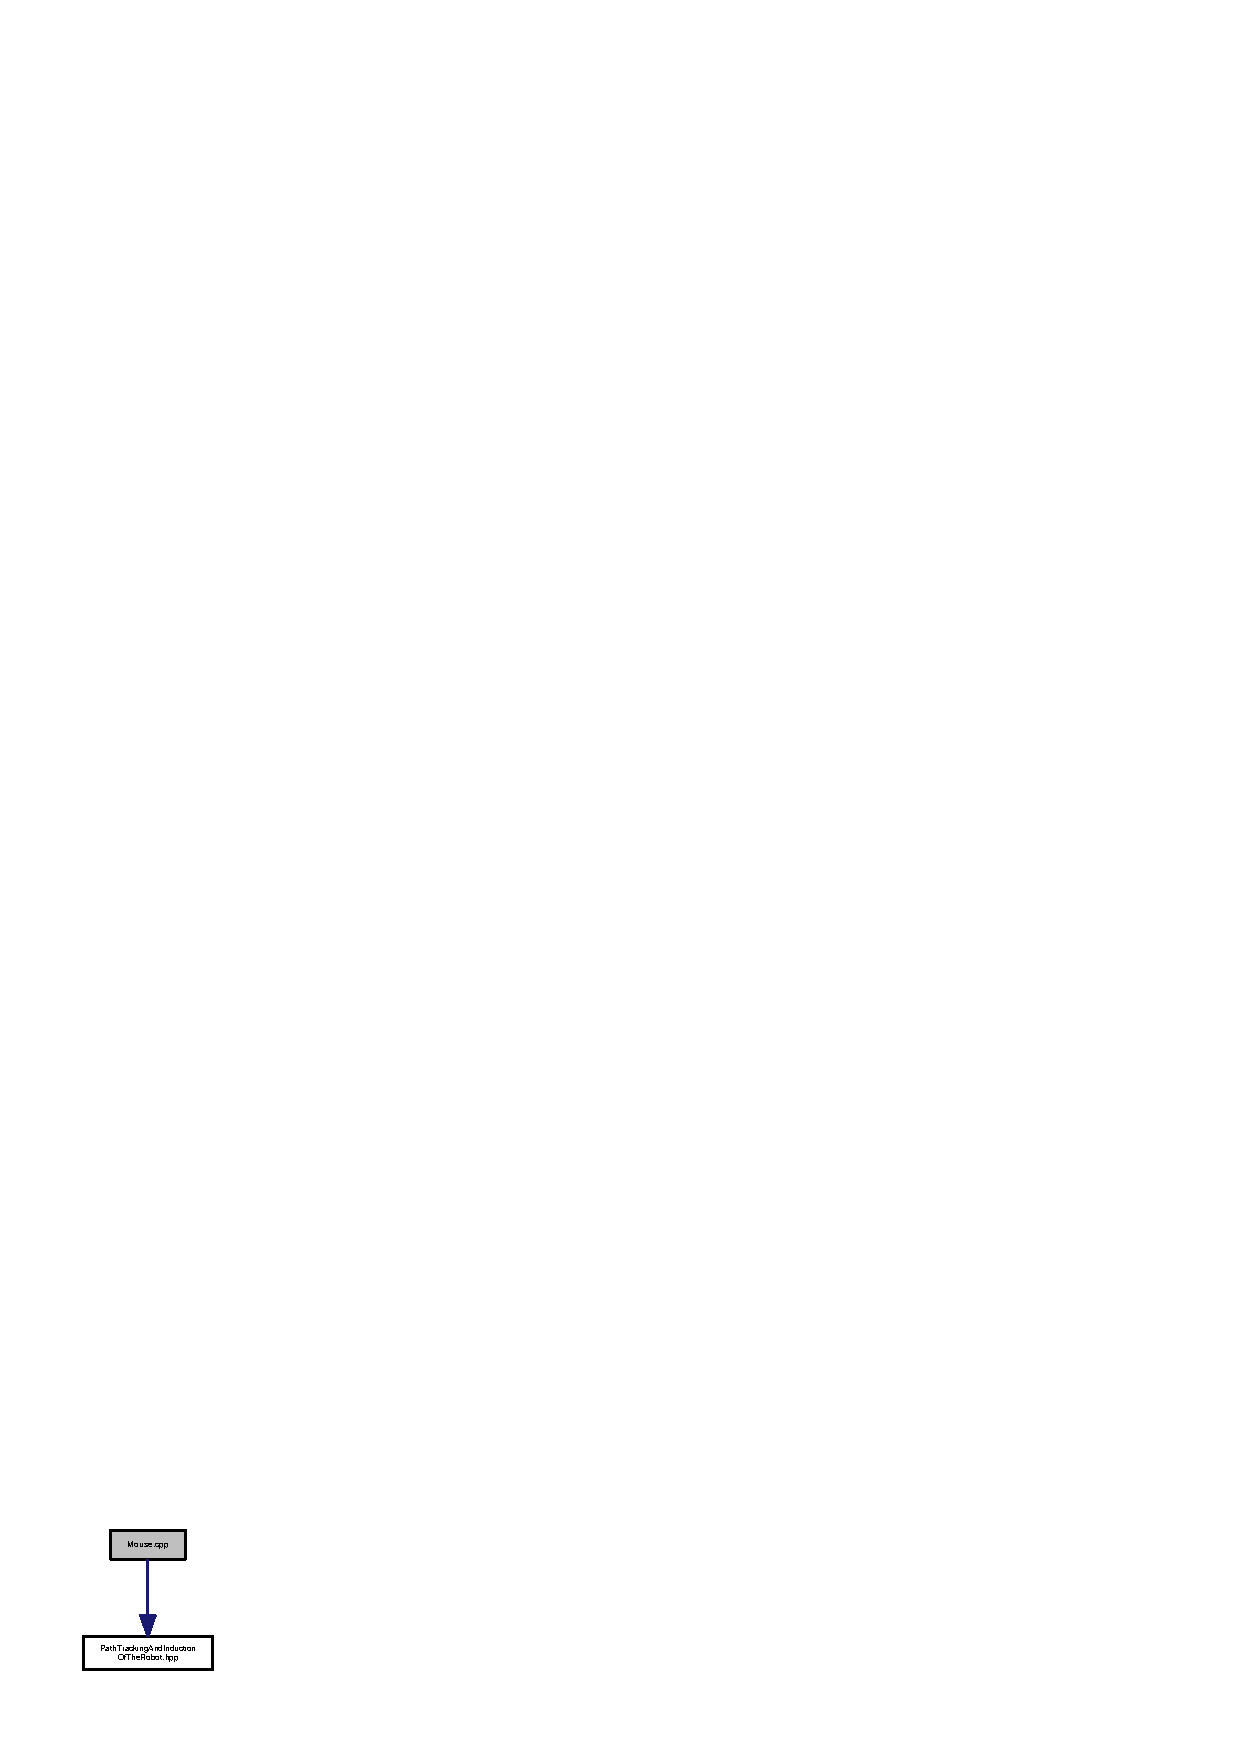
\includegraphics[width=106pt]{_mouse_8cpp__incl}
\end{center}
\end{figure}
\subsection*{関数}
\begin{DoxyCompactItemize}
\item 
void {\bf on\-Mouse} (int event, int x, int y, int flags, void $\ast$param)
\begin{DoxyCompactList}\small\item\em メソッドon\-Mouse().マウス左クリックで座標を取得するメソッド \end{DoxyCompactList}\end{DoxyCompactItemize}


\subsection{関数詳解}
\index{Mouse.\-cpp@{Mouse.\-cpp}!on\-Mouse@{on\-Mouse}}
\index{on\-Mouse@{on\-Mouse}!Mouse.cpp@{Mouse.\-cpp}}
\subsubsection[{on\-Mouse}]{\setlength{\rightskip}{0pt plus 5cm}void on\-Mouse (
\begin{DoxyParamCaption}
\item[{int}]{event, }
\item[{int}]{x, }
\item[{int}]{y, }
\item[{int}]{flags, }
\item[{void $\ast$}]{param}
\end{DoxyParamCaption}
)}\label{_mouse_8cpp_ab6ccc6c8d80970d4178c943533533860}


メソッドon\-Mouse().マウス左クリックで座標を取得するメソッド 

マウス操作


\begin{DoxyParams}{引数}
{\em event} & int 型.イベント \\
\hline
{\em x} & int型.x座標 \\
\hline
{\em y} & int型.y座標 \\
\hline
{\em flags} & int型.フラグ \\
\hline
{\em param} & void$\ast$型.その他パラメータ \\
\hline
\end{DoxyParams}


 Mouse.\-cpp の 19 行目に定義があります。



参照先 image, origin, selection, select\-Object, track\-Object.


\section{Path\-Tracking\-And\-Induction\-Of\-The\-Robot.\-hpp ファイル}
\label{_path_tracking_and_induction_of_the_robot_8hpp}\index{Path\-Tracking\-And\-Induction\-Of\-The\-Robot.\-hpp@{Path\-Tracking\-And\-Induction\-Of\-The\-Robot.\-hpp}}
\subsection*{クラス}
\begin{DoxyCompactItemize}
\item 
struct {\bf Point3}
\item 
struct {\bf output\-Data}
\item 
struct {\bf Do\-F}
\item 
struct {\bf Attitude\-Angle}
\end{DoxyCompactItemize}
\subsection*{型定義}
\begin{DoxyCompactItemize}
\item 
typedef struct {\bf Point3} {\bf Point3ius}
\item 
typedef struct {\bf output\-Data} {\bf output\-Data}
\item 
typedef struct {\bf Do\-F} {\bf Do\-F6d}
\item 
typedef struct {\bf Attitude\-Angle} {\bf Attitude\-Angle3d}
\end{DoxyCompactItemize}
\subsection*{関数}
\begin{DoxyCompactItemize}
\item 
void {\bf on\-Mouse} (int event, int x, int y, int, void $\ast$)
\begin{DoxyCompactList}\small\item\em マウス操作 \end{DoxyCompactList}\end{DoxyCompactItemize}
\subsection*{変数}
\begin{DoxyCompactItemize}
\item 
Mat {\bf image}
\begin{DoxyCompactList}\small\item\em R\-G\-B画像格納用の変数 \end{DoxyCompactList}\item 
char {\bf directory\-Name} [{\bf N\-O\-C}]
\begin{DoxyCompactList}\small\item\em フォルダ名 \end{DoxyCompactList}\item 
bool {\bf select\-Object}
\begin{DoxyCompactList}\small\item\em オブジェクト選択 \end{DoxyCompactList}\item 
int {\bf track\-Object}
\begin{DoxyCompactList}\small\item\em 追跡するオブジェクト \end{DoxyCompactList}\item 
Point {\bf origin}
\begin{DoxyCompactList}\small\item\em オリジナルの座標 \end{DoxyCompactList}\item 
Rect {\bf selection}
\begin{DoxyCompactList}\small\item\em 選択 \end{DoxyCompactList}\item 
int {\bf save\-\_\-count}
\end{DoxyCompactItemize}


\subsection{型定義詳解}
\index{Path\-Tracking\-And\-Induction\-Of\-The\-Robot.\-hpp@{Path\-Tracking\-And\-Induction\-Of\-The\-Robot.\-hpp}!Attitude\-Angle3d@{Attitude\-Angle3d}}
\index{Attitude\-Angle3d@{Attitude\-Angle3d}!PathTrackingAndInductionOfTheRobot.hpp@{Path\-Tracking\-And\-Induction\-Of\-The\-Robot.\-hpp}}
\subsubsection[{Attitude\-Angle3d}]{\setlength{\rightskip}{0pt plus 5cm}typedef struct {\bf Attitude\-Angle} {\bf Attitude\-Angle3d}}\label{_path_tracking_and_induction_of_the_robot_8hpp_a4860903646946a52474a935518d26b08}
\index{Path\-Tracking\-And\-Induction\-Of\-The\-Robot.\-hpp@{Path\-Tracking\-And\-Induction\-Of\-The\-Robot.\-hpp}!Do\-F6d@{Do\-F6d}}
\index{Do\-F6d@{Do\-F6d}!PathTrackingAndInductionOfTheRobot.hpp@{Path\-Tracking\-And\-Induction\-Of\-The\-Robot.\-hpp}}
\subsubsection[{Do\-F6d}]{\setlength{\rightskip}{0pt plus 5cm}typedef struct {\bf Do\-F} {\bf Do\-F6d}}\label{_path_tracking_and_induction_of_the_robot_8hpp_a33b77e4ea1c0ec898f240665aba2a93c}
\index{Path\-Tracking\-And\-Induction\-Of\-The\-Robot.\-hpp@{Path\-Tracking\-And\-Induction\-Of\-The\-Robot.\-hpp}!output\-Data@{output\-Data}}
\index{output\-Data@{output\-Data}!PathTrackingAndInductionOfTheRobot.hpp@{Path\-Tracking\-And\-Induction\-Of\-The\-Robot.\-hpp}}
\subsubsection[{output\-Data}]{\setlength{\rightskip}{0pt plus 5cm}typedef struct {\bf output\-Data} {\bf output\-Data}}\label{_path_tracking_and_induction_of_the_robot_8hpp_a9618d6d926e1cc639647588117793210}
\index{Path\-Tracking\-And\-Induction\-Of\-The\-Robot.\-hpp@{Path\-Tracking\-And\-Induction\-Of\-The\-Robot.\-hpp}!Point3ius@{Point3ius}}
\index{Point3ius@{Point3ius}!PathTrackingAndInductionOfTheRobot.hpp@{Path\-Tracking\-And\-Induction\-Of\-The\-Robot.\-hpp}}
\subsubsection[{Point3ius}]{\setlength{\rightskip}{0pt plus 5cm}typedef struct {\bf Point3} {\bf Point3ius}}\label{_path_tracking_and_induction_of_the_robot_8hpp_a9cd09b6cf0b036e8fe8d70d17d7fbe1f}


\subsection{関数詳解}
\index{Path\-Tracking\-And\-Induction\-Of\-The\-Robot.\-hpp@{Path\-Tracking\-And\-Induction\-Of\-The\-Robot.\-hpp}!on\-Mouse@{on\-Mouse}}
\index{on\-Mouse@{on\-Mouse}!PathTrackingAndInductionOfTheRobot.hpp@{Path\-Tracking\-And\-Induction\-Of\-The\-Robot.\-hpp}}
\subsubsection[{on\-Mouse}]{\setlength{\rightskip}{0pt plus 5cm}void on\-Mouse (
\begin{DoxyParamCaption}
\item[{int}]{event, }
\item[{int}]{x, }
\item[{int}]{y, }
\item[{int}]{, }
\item[{void $\ast$}]{}
\end{DoxyParamCaption}
)}\label{_path_tracking_and_induction_of_the_robot_8hpp_a6c81aa00b4dcf0cbae98a14c37683ed9}


マウス操作 



 Mouse.\-cpp の 12 行目に定義があります。



参照先 image, origin, selection, select\-Object, track\-Object.


\begin{DoxyCode}
13 \{
14     \textcolor{keywordflow}{if} (selectObject)
15     \{
16         selection.x = MIN(x, origin.x);
17         selection.y = MIN(y, origin.y);
18         selection.width = abs(x - origin.x);
19         selection.height = abs(y - origin.y);
20         selection &= Rect(0, 0, image.cols, image.rows);
21     \}
22 
23     \textcolor{keywordflow}{switch} (event)
24     \{
25     \textcolor{keywordflow}{case} CV\_EVENT\_LBUTTONDOWN:
26         origin = Point(x, y);
27         selection = Rect(x, y, 0, 0);
28         selectObject = \textcolor{keyword}{true};
29         \textcolor{keywordflow}{break};
30     \textcolor{keywordflow}{case} CV\_EVENT\_LBUTTONUP:
31         selectObject = \textcolor{keyword}{false};
32         \textcolor{keywordflow}{if} (selection.width > 0 && selection.height > 0)
33         \{
34             trackObject = -1;
35         \}
36         \textcolor{keywordflow}{break};
37     \}
38 
39     \textcolor{keywordflow}{return};
40 \}\end{DoxyCode}


\subsection{変数詳解}
\index{Path\-Tracking\-And\-Induction\-Of\-The\-Robot.\-hpp@{Path\-Tracking\-And\-Induction\-Of\-The\-Robot.\-hpp}!directory\-Name@{directory\-Name}}
\index{directory\-Name@{directory\-Name}!PathTrackingAndInductionOfTheRobot.hpp@{Path\-Tracking\-And\-Induction\-Of\-The\-Robot.\-hpp}}
\subsubsection[{directory\-Name}]{\setlength{\rightskip}{0pt plus 5cm}char directory\-Name[{\bf N\-O\-C}]}\label{_path_tracking_and_induction_of_the_robot_8hpp_abefb498e9a643f68bb3d37c22953ddad}


フォルダ名 



 main.\-cpp の 23 行目に定義があります。



参照元 System\-::end\-Message(), Drawing\-::gnuplot\-Script(), Drawing\-::gnuplot\-Script\-Co\-G(), Drawing\-::gnuplot\-Script\-E\-V3\-Route(), Drawing\-::gnuplot\-Script\-E\-V3\-Unit(), System\-::make\-Directory(), System\-::open\-Directory(), System\-::output\-All\-Data(), System\-::output\-Video(), Drawing\-::plot3\-D(), Drawing\-::plot3\-D\-Real\-Time(), System\-::remove\-Directory(), System\-::save\-Data\-Continuously(), System\-::save\-Data\-Every\-Enter\-Key().

\index{Path\-Tracking\-And\-Induction\-Of\-The\-Robot.\-hpp@{Path\-Tracking\-And\-Induction\-Of\-The\-Robot.\-hpp}!image@{image}}
\index{image@{image}!PathTrackingAndInductionOfTheRobot.hpp@{Path\-Tracking\-And\-Induction\-Of\-The\-Robot.\-hpp}}
\subsubsection[{image}]{\setlength{\rightskip}{0pt plus 5cm}Mat image}\label{_path_tracking_and_induction_of_the_robot_8hpp_aabb27b8973575043030df51be47cd24a}


R\-G\-B画像格納用の変数 



 main.\-cpp の 21 行目に定義があります。



参照元 Kinect\-::get\-Point\-Cloud(), main(), on\-Mouse().

\index{Path\-Tracking\-And\-Induction\-Of\-The\-Robot.\-hpp@{Path\-Tracking\-And\-Induction\-Of\-The\-Robot.\-hpp}!origin@{origin}}
\index{origin@{origin}!PathTrackingAndInductionOfTheRobot.hpp@{Path\-Tracking\-And\-Induction\-Of\-The\-Robot.\-hpp}}
\subsubsection[{origin}]{\setlength{\rightskip}{0pt plus 5cm}Point origin}\label{_path_tracking_and_induction_of_the_robot_8hpp_a903d0d8820c696aaa1170c50deb3633f}


オリジナルの座標 



 main.\-cpp の 28 行目に定義があります。



参照元 on\-Mouse().

\index{Path\-Tracking\-And\-Induction\-Of\-The\-Robot.\-hpp@{Path\-Tracking\-And\-Induction\-Of\-The\-Robot.\-hpp}!save\-\_\-count@{save\-\_\-count}}
\index{save\-\_\-count@{save\-\_\-count}!PathTrackingAndInductionOfTheRobot.hpp@{Path\-Tracking\-And\-Induction\-Of\-The\-Robot.\-hpp}}
\subsubsection[{save\-\_\-count}]{\setlength{\rightskip}{0pt plus 5cm}int save\-\_\-count}\label{_path_tracking_and_induction_of_the_robot_8hpp_aacae5d304dcef5f6bbf0fe5030e50626}


 main.\-cpp の 32 行目に定義があります。



参照元 Drawing\-::gnuplot\-Script\-E\-V3\-Unit(), main(), System\-::save\-Data\-Every\-Enter\-Key().

\index{Path\-Tracking\-And\-Induction\-Of\-The\-Robot.\-hpp@{Path\-Tracking\-And\-Induction\-Of\-The\-Robot.\-hpp}!selection@{selection}}
\index{selection@{selection}!PathTrackingAndInductionOfTheRobot.hpp@{Path\-Tracking\-And\-Induction\-Of\-The\-Robot.\-hpp}}
\subsubsection[{selection}]{\setlength{\rightskip}{0pt plus 5cm}Rect selection}\label{_path_tracking_and_induction_of_the_robot_8hpp_a15633c47538e3790df1e008a7f6dbfea}


選択 



 main.\-cpp の 29 行目に定義があります。



参照元 on\-Mouse().

\index{Path\-Tracking\-And\-Induction\-Of\-The\-Robot.\-hpp@{Path\-Tracking\-And\-Induction\-Of\-The\-Robot.\-hpp}!select\-Object@{select\-Object}}
\index{select\-Object@{select\-Object}!PathTrackingAndInductionOfTheRobot.hpp@{Path\-Tracking\-And\-Induction\-Of\-The\-Robot.\-hpp}}
\subsubsection[{select\-Object}]{\setlength{\rightskip}{0pt plus 5cm}bool select\-Object}\label{_path_tracking_and_induction_of_the_robot_8hpp_a71a276a0dc4ef6aa35740b58f10bcb39}


オブジェクト選択 



 main.\-cpp の 26 行目に定義があります。



参照元 on\-Mouse().

\index{Path\-Tracking\-And\-Induction\-Of\-The\-Robot.\-hpp@{Path\-Tracking\-And\-Induction\-Of\-The\-Robot.\-hpp}!track\-Object@{track\-Object}}
\index{track\-Object@{track\-Object}!PathTrackingAndInductionOfTheRobot.hpp@{Path\-Tracking\-And\-Induction\-Of\-The\-Robot.\-hpp}}
\subsubsection[{track\-Object}]{\setlength{\rightskip}{0pt plus 5cm}int track\-Object}\label{_path_tracking_and_induction_of_the_robot_8hpp_a88f176e4e65e22a17093a8cd24003a66}


追跡するオブジェクト 



 main.\-cpp の 27 行目に定義があります。



参照元 on\-Mouse().


\section{Point\-Cloud\-Library.\-cpp ファイル}
\label{_point_cloud_library_8cpp}\index{Point\-Cloud\-Library.\-cpp@{Point\-Cloud\-Library.\-cpp}}
{\ttfamily \#include \char`\"{}Path\-Tracking\-And\-Induction\-Of\-The\-Robot.\-hpp\char`\"{}}\\*
{\ttfamily \#include \char`\"{}Point\-Cloud\-Library.\-hpp\char`\"{}}\\*
Point\-Cloud\-Library.\-cpp の依存先関係図\-:\nopagebreak
\begin{figure}[H]
\begin{center}
\leavevmode
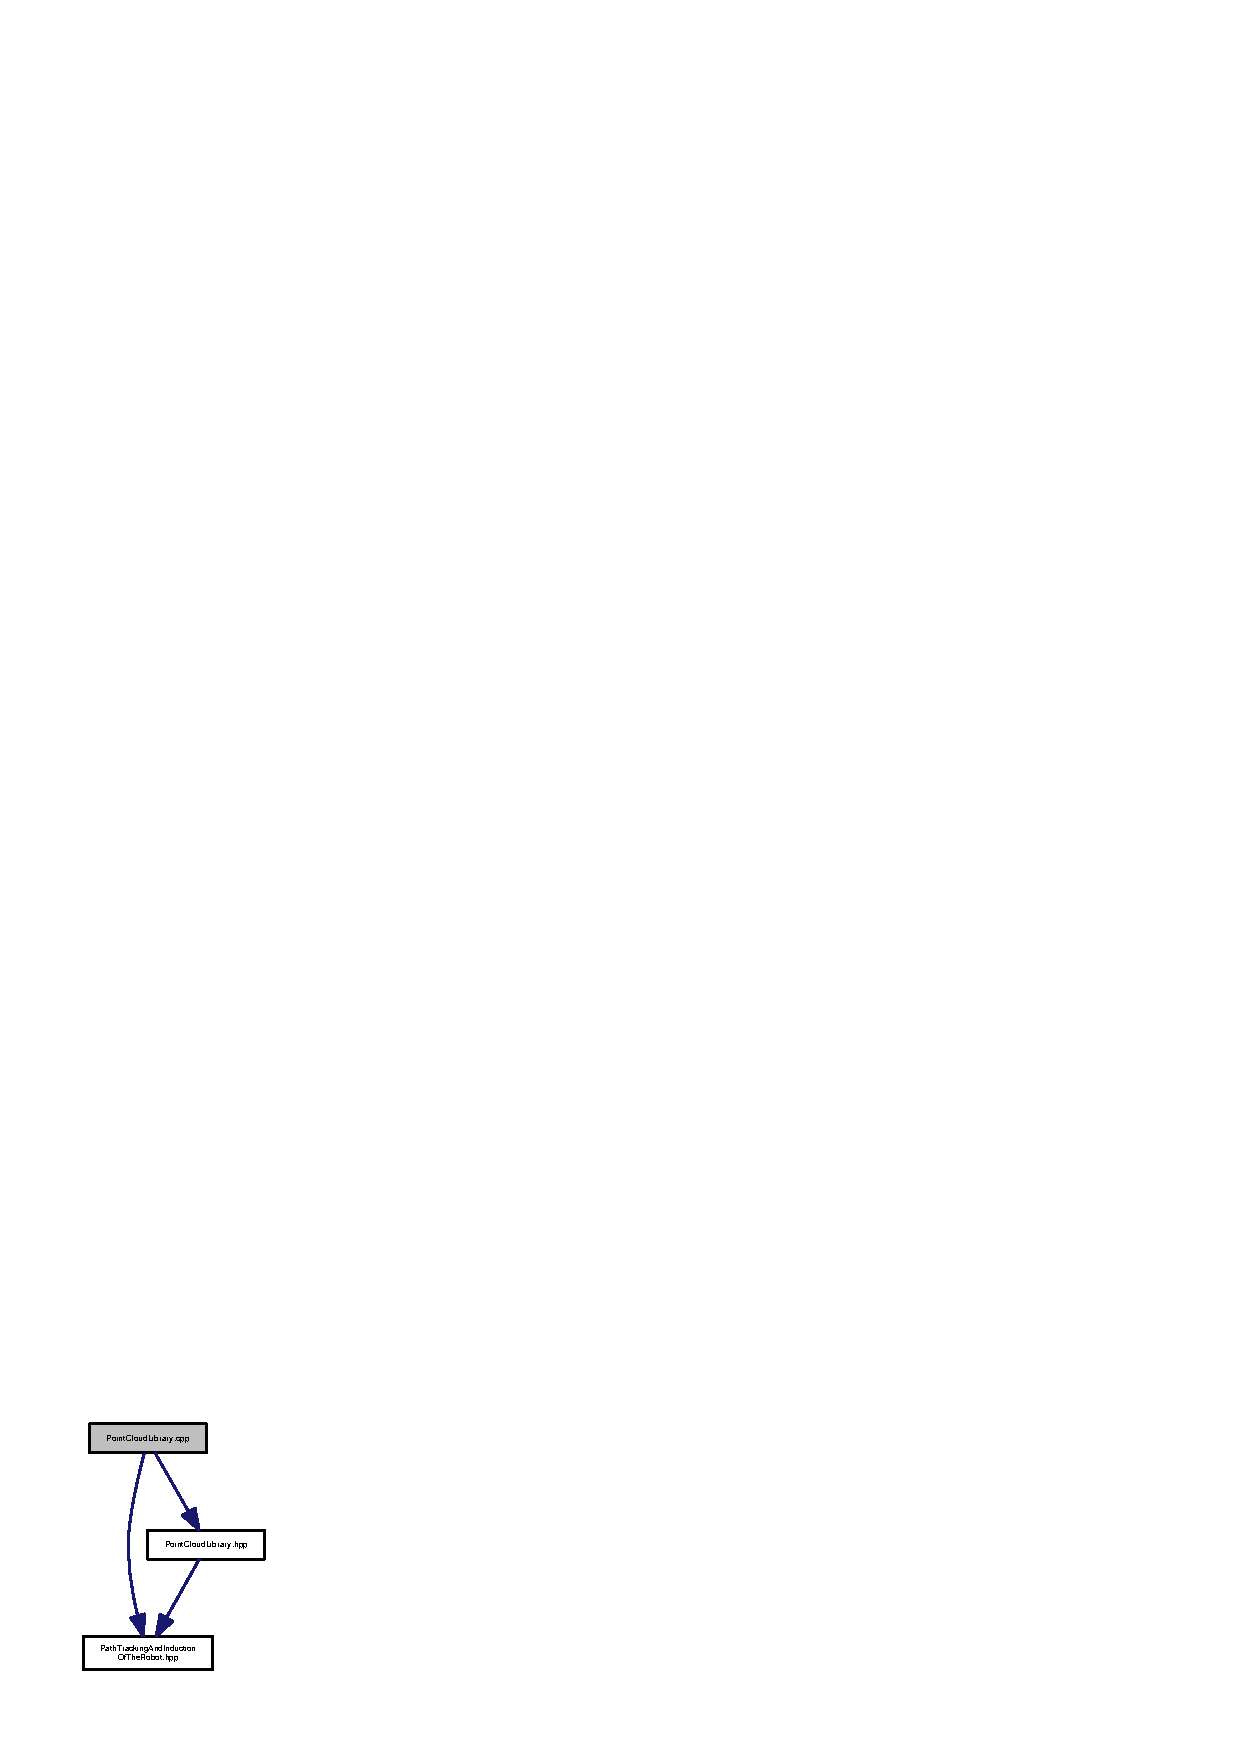
\includegraphics[width=131pt]{_point_cloud_library_8cpp__incl}
\end{center}
\end{figure}

\section{Point\-Cloud\-Library.\-hpp ファイル}
\label{_point_cloud_library_8hpp}\index{Point\-Cloud\-Library.\-hpp@{Point\-Cloud\-Library.\-hpp}}
{\ttfamily \#include \char`\"{}Path\-Tracking\-And\-Induction\-Of\-The\-Robot.\-hpp\char`\"{}}\\*
Point\-Cloud\-Library.\-hpp の依存先関係図\-:\nopagebreak
\begin{figure}[H]
\begin{center}
\leavevmode
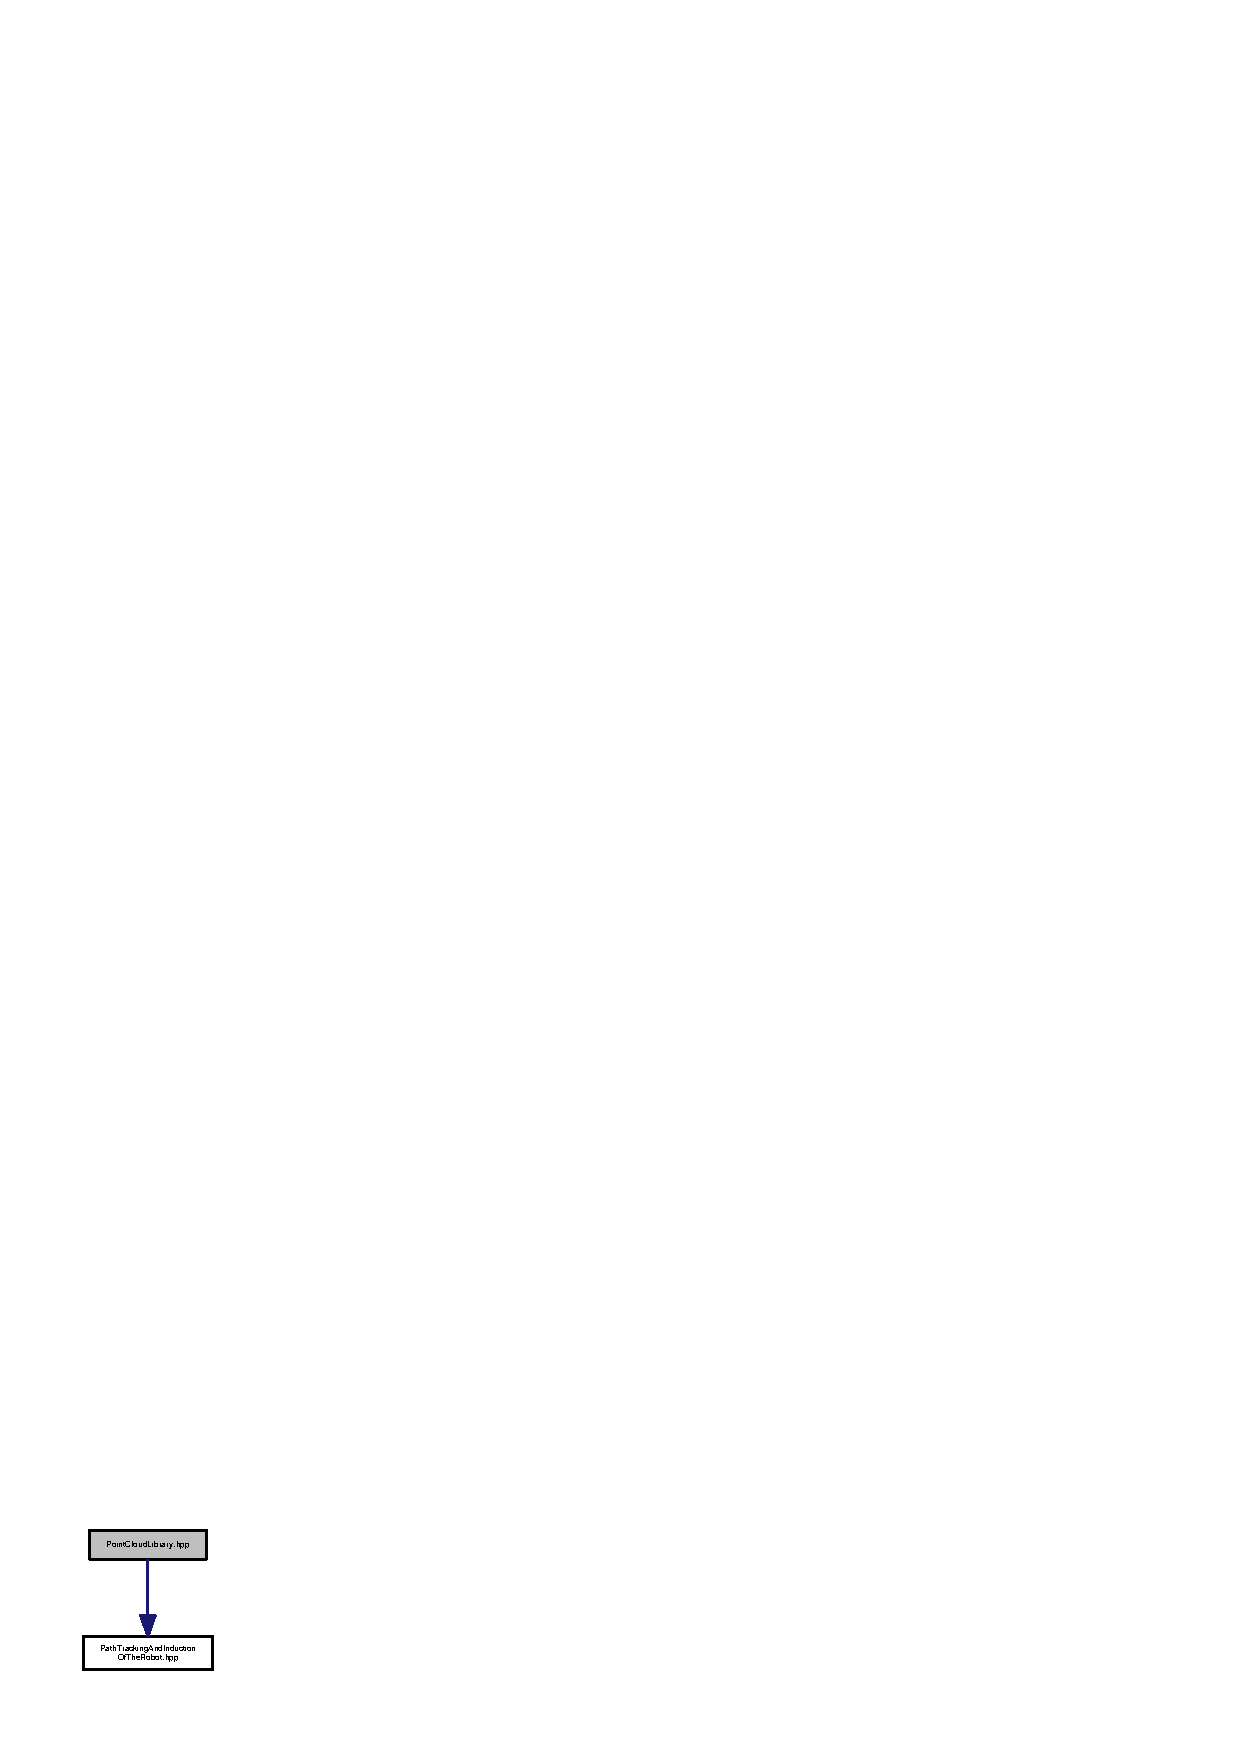
\includegraphics[width=106pt]{_point_cloud_library_8hpp__incl}
\end{center}
\end{figure}
被依存関係図\-:\nopagebreak
\begin{figure}[H]
\begin{center}
\leavevmode
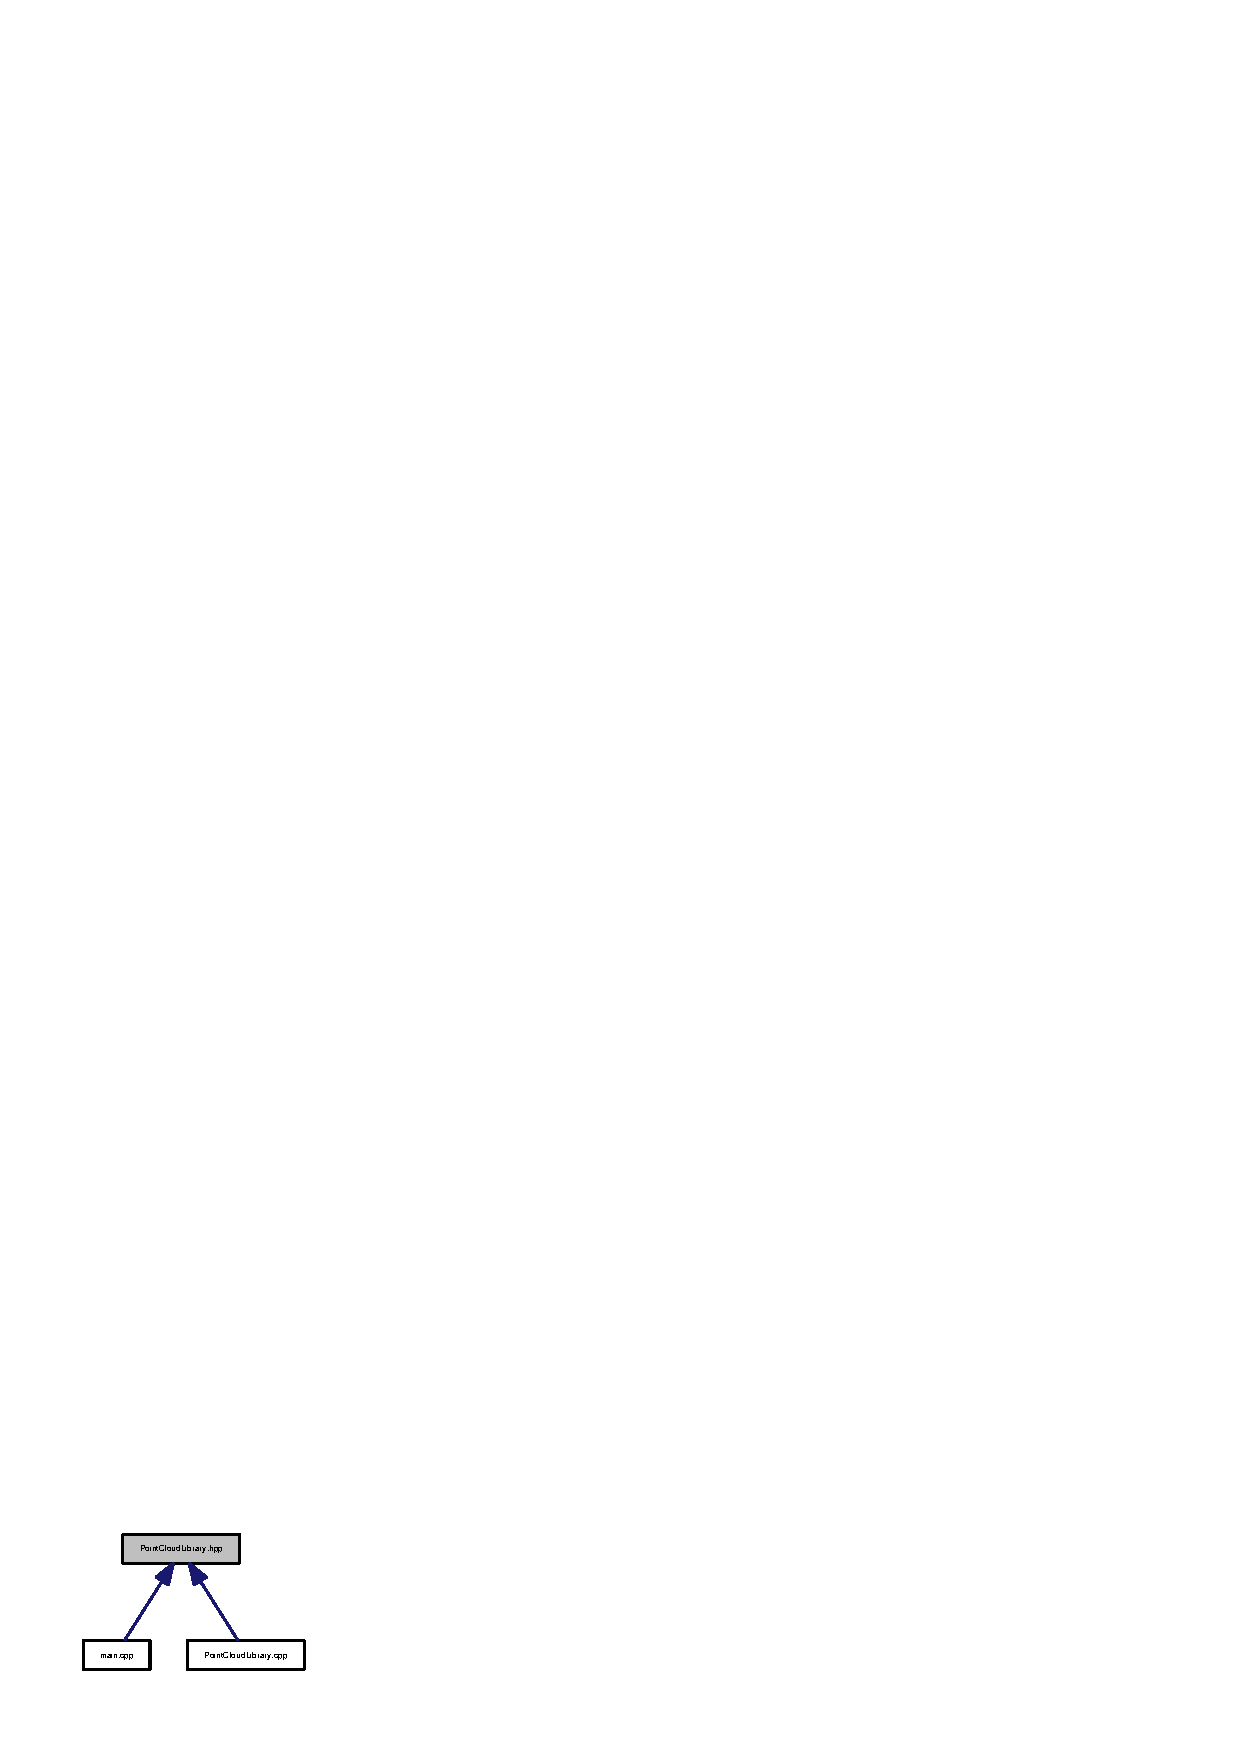
\includegraphics[width=150pt]{_point_cloud_library_8hpp__dep__incl}
\end{center}
\end{figure}
\subsection*{クラス}
\begin{DoxyCompactItemize}
\item 
class {\bf Point\-Cloud\-Library}
\begin{DoxyCompactList}\small\item\em 点群処理を行うクラス \end{DoxyCompactList}\end{DoxyCompactItemize}

\section{stdafx.\-cpp ファイル}
\label{stdafx_8cpp}\index{stdafx.\-cpp@{stdafx.\-cpp}}

\section{stdafx.\-h ファイル}
\label{stdafx_8h}\index{stdafx.\-h@{stdafx.\-h}}
{\ttfamily \#include $<$iostream$>$}\\*
{\ttfamily \#include $<$sstream$>$}\\*
{\ttfamily \#include $<$fstream$>$}\\*
{\ttfamily \#include $<$string$>$}\\*
{\ttfamily \#include $<$stdio.\-h$>$}\\*
{\ttfamily \#include $<$stdlib.\-h$>$}\\*
{\ttfamily \#include $<$direct.\-h$>$}\\*
{\ttfamily \#include $<$math.\-h$>$}\\*
{\ttfamily \#include $<$ctype.\-h$>$}\\*
{\ttfamily \#include $<$sys/stat.\-h$>$}\\*
{\ttfamily \#include $<$Windows.\-h$>$}\\*
{\ttfamily \#include $<$mmsystem.\-h$>$}\\*
{\ttfamily \#include $<$Nui\-Api.\-h$>$}\\*
{\ttfamily \#include $<$opencv2\textbackslash{}opencv.\-hpp$>$}\\*
{\ttfamily \#include $<$opencv2\textbackslash{}core\textbackslash{}core.\-hpp$>$}\\*
{\ttfamily \#include $<$opencv2\textbackslash{}highgui\textbackslash{}highgui.\-hpp$>$}\\*
{\ttfamily \#include $<$opencv2\textbackslash{}imgproc\textbackslash{}imgproc.\-hpp$>$}\\*
{\ttfamily \#include $<$opencv2\textbackslash{}video\textbackslash{}tracking.\-hpp$>$}\\*
{\ttfamily \#include $<$opencv2\textbackslash{}flann\textbackslash{}flann.\-hpp$>$}\\*
{\ttfamily \#include $<$pcl\textbackslash{}point\-\_\-types.\-h$>$}\\*
{\ttfamily \#include $<$pcl\textbackslash{}point\-\_\-cloud.\-h$>$}\\*
{\ttfamily \#include $<$pcl\textbackslash{}io\textbackslash{}io.\-h$>$}\\*
{\ttfamily \#include $<$pcl\textbackslash{}io\textbackslash{}pcd\-\_\-io.\-h$>$}\\*
{\ttfamily \#include $<$pcl\textbackslash{}io\textbackslash{}ply\-\_\-io.\-h$>$}\\*
{\ttfamily \#include $<$pcl\textbackslash{}common\textbackslash{}common\-\_\-headers.\-h$>$}\\*
{\ttfamily \#include $<$pcl\textbackslash{}visualization\textbackslash{}cloud\-\_\-viewer.\-h$>$}\\*
{\ttfamily \#include $<$pcl\textbackslash{}visualization\textbackslash{}pcl\-\_\-visualizer.\-h$>$}\\*
{\ttfamily \#include $<$pcl\textbackslash{}filters\textbackslash{}passthrough.\-h$>$}\\*
{\ttfamily \#include $<$pcl\textbackslash{}filters\textbackslash{}statistical\-\_\-outlier\-\_\-removal.\-h$>$}\\*
{\ttfamily \#include $<$pcl\textbackslash{}filters\textbackslash{}radius\-\_\-outlier\-\_\-removal.\-h$>$}\\*
{\ttfamily \#include $<$pcl\textbackslash{}kdtree\textbackslash{}kdtree\-\_\-flann.\-h$>$}\\*
{\ttfamily \#include $<$pcl\textbackslash{}surface\textbackslash{}mls.\-h$>$}\\*
{\ttfamily \#include $<$pcl\textbackslash{}filters\textbackslash{}voxel\-\_\-grid.\-h$>$}\\*
{\ttfamily \#include $<$pcl\textbackslash{}\-Model\-Coefficients.\-h$>$}\\*
{\ttfamily \#include $<$pcl\textbackslash{}sample\-\_\-consensus\textbackslash{}method\-\_\-types.\-h$>$}\\*
{\ttfamily \#include $<$pcl\textbackslash{}sample\-\_\-consensus\textbackslash{}model\-\_\-types.\-h$>$}\\*
{\ttfamily \#include $<$pcl\textbackslash{}segmentation\textbackslash{}sac\-\_\-segmentation.\-h$>$}\\*
{\ttfamily \#include $<$pcl\textbackslash{}filters\textbackslash{}extract\-\_\-indices.\-h$>$}\\*
{\ttfamily \#include $<$pcl\textbackslash{}features\textbackslash{}normal\-\_\-3d.\-h$>$}\\*
{\ttfamily \#include $<$pcl\textbackslash{}segmentation\textbackslash{}extract\-\_\-clusters.\-h$>$}\\*
{\ttfamily \#include $<$boost\textbackslash{}thread\textbackslash{}thread.\-hpp$>$}\\*
{\ttfamily \#include $<$pcl\textbackslash{}registration\textbackslash{}icp.\-h$>$}\\*
{\ttfamily \#include $<$pcl\textbackslash{}\-P\-C\-L\-Point\-Field.\-h$>$}\\*
\subsection*{マクロ定義}
\begin{DoxyCompactItemize}
\item 
\#define {\bf \-\_\-\-C\-R\-T\-\_\-\-S\-E\-C\-U\-R\-E\-\_\-\-N\-O\-\_\-\-W\-A\-R\-N\-I\-N\-G\-S}
\item 
\#define {\bf W\-I\-D\-T\-H}~640
\begin{DoxyCompactList}\small\item\em $<$名前空間 \end{DoxyCompactList}\item 
\#define {\bf H\-E\-I\-G\-H\-T}~480
\begin{DoxyCompactList}\small\item\em 画像の高さ \end{DoxyCompactList}\item 
\#define {\bf A\-L\-L\-P\-I\-X\-E\-L}~{\bf W\-I\-D\-T\-H}$\ast${\bf H\-E\-I\-G\-H\-T}
\begin{DoxyCompactList}\small\item\em 1フレームの全ピクセル数 \end{DoxyCompactList}\item 
\#define {\bf N\-O\-C}~64
\begin{DoxyCompactList}\small\item\em Number of Characters.(ファイルの名前を付けるときの文字数制限) \end{DoxyCompactList}\item 
\#define {\bf O\-U\-T\-P\-U\-T\-D\-A\-T\-A\-\_\-\-M\-A\-X}~10000
\begin{DoxyCompactList}\small\item\em 出力するデータの上限 \end{DoxyCompactList}\end{DoxyCompactItemize}


\subsection{マクロ定義詳解}
\index{stdafx.\-h@{stdafx.\-h}!\-\_\-\-C\-R\-T\-\_\-\-S\-E\-C\-U\-R\-E\-\_\-\-N\-O\-\_\-\-W\-A\-R\-N\-I\-N\-G\-S@{\-\_\-\-C\-R\-T\-\_\-\-S\-E\-C\-U\-R\-E\-\_\-\-N\-O\-\_\-\-W\-A\-R\-N\-I\-N\-G\-S}}
\index{\-\_\-\-C\-R\-T\-\_\-\-S\-E\-C\-U\-R\-E\-\_\-\-N\-O\-\_\-\-W\-A\-R\-N\-I\-N\-G\-S@{\-\_\-\-C\-R\-T\-\_\-\-S\-E\-C\-U\-R\-E\-\_\-\-N\-O\-\_\-\-W\-A\-R\-N\-I\-N\-G\-S}!stdafx.h@{stdafx.\-h}}
\subsubsection[{\-\_\-\-C\-R\-T\-\_\-\-S\-E\-C\-U\-R\-E\-\_\-\-N\-O\-\_\-\-W\-A\-R\-N\-I\-N\-G\-S}]{\setlength{\rightskip}{0pt plus 5cm}\#define \-\_\-\-C\-R\-T\-\_\-\-S\-E\-C\-U\-R\-E\-\_\-\-N\-O\-\_\-\-W\-A\-R\-N\-I\-N\-G\-S}\label{stdafx_8h_af08ec37a8c99d747fb60fa15bc28678b}


 stdafx.\-h の 8 行目に定義があります。

\index{stdafx.\-h@{stdafx.\-h}!A\-L\-L\-P\-I\-X\-E\-L@{A\-L\-L\-P\-I\-X\-E\-L}}
\index{A\-L\-L\-P\-I\-X\-E\-L@{A\-L\-L\-P\-I\-X\-E\-L}!stdafx.h@{stdafx.\-h}}
\subsubsection[{A\-L\-L\-P\-I\-X\-E\-L}]{\setlength{\rightskip}{0pt plus 5cm}\#define A\-L\-L\-P\-I\-X\-E\-L~{\bf W\-I\-D\-T\-H}$\ast${\bf H\-E\-I\-G\-H\-T}}\label{stdafx_8h_ada27e1c35871e9e6118bd9818362f01e}


1フレームの全ピクセル数 



 stdafx.\-h の 78 行目に定義があります。

\index{stdafx.\-h@{stdafx.\-h}!H\-E\-I\-G\-H\-T@{H\-E\-I\-G\-H\-T}}
\index{H\-E\-I\-G\-H\-T@{H\-E\-I\-G\-H\-T}!stdafx.h@{stdafx.\-h}}
\subsubsection[{H\-E\-I\-G\-H\-T}]{\setlength{\rightskip}{0pt plus 5cm}\#define H\-E\-I\-G\-H\-T~480}\label{stdafx_8h_aed89bd71aee8be823e8a20ec4e093c1e}


画像の高さ 



 stdafx.\-h の 77 行目に定義があります。

\index{stdafx.\-h@{stdafx.\-h}!N\-O\-C@{N\-O\-C}}
\index{N\-O\-C@{N\-O\-C}!stdafx.h@{stdafx.\-h}}
\subsubsection[{N\-O\-C}]{\setlength{\rightskip}{0pt plus 5cm}\#define N\-O\-C~64}\label{stdafx_8h_a5d8ba032e2fdf7b2561f508164124f3e}


Number of Characters.(ファイルの名前を付けるときの文字数制限) 



 stdafx.\-h の 79 行目に定義があります。



参照元 Drawing\-::gnuplot\-Script(), Drawing\-::gnuplot\-Script\-Co\-G(), Drawing\-::gnuplot\-Script\-E\-V3\-Route(), Drawing\-::gnuplot\-Script\-E\-V3\-Unit(), System\-::make\-Directory(), System\-::open\-Directory(), System\-::output\-All\-Data(), System\-::output\-Video(), Drawing\-::plot3\-D\-Real\-Time(), System\-::remove\-Directory(), System\-::save\-Data\-Continuously(), System\-::save\-Data\-Every\-Enter\-Key().

\index{stdafx.\-h@{stdafx.\-h}!O\-U\-T\-P\-U\-T\-D\-A\-T\-A\-\_\-\-M\-A\-X@{O\-U\-T\-P\-U\-T\-D\-A\-T\-A\-\_\-\-M\-A\-X}}
\index{O\-U\-T\-P\-U\-T\-D\-A\-T\-A\-\_\-\-M\-A\-X@{O\-U\-T\-P\-U\-T\-D\-A\-T\-A\-\_\-\-M\-A\-X}!stdafx.h@{stdafx.\-h}}
\subsubsection[{O\-U\-T\-P\-U\-T\-D\-A\-T\-A\-\_\-\-M\-A\-X}]{\setlength{\rightskip}{0pt plus 5cm}\#define O\-U\-T\-P\-U\-T\-D\-A\-T\-A\-\_\-\-M\-A\-X~10000}\label{stdafx_8h_af962cd28db9fad108f1e02b7f90192b7}


出力するデータの上限 



 stdafx.\-h の 80 行目に定義があります。

\index{stdafx.\-h@{stdafx.\-h}!W\-I\-D\-T\-H@{W\-I\-D\-T\-H}}
\index{W\-I\-D\-T\-H@{W\-I\-D\-T\-H}!stdafx.h@{stdafx.\-h}}
\subsubsection[{W\-I\-D\-T\-H}]{\setlength{\rightskip}{0pt plus 5cm}\#define W\-I\-D\-T\-H~640}\label{stdafx_8h_a241aeeb764887ae5e3de58b98f04b16d}


$<$名前空間 

画像の幅 

 stdafx.\-h の 76 行目に定義があります。


\section{System.\-cpp ファイル}
\label{_system_8cpp}\index{System.\-cpp@{System.\-cpp}}
{\ttfamily \#include \char`\"{}Path\-Tracking\-And\-Induction\-Of\-The\-Robot.\-hpp\char`\"{}}\\*
{\ttfamily \#include \char`\"{}System.\-hpp\char`\"{}}\\*

\section{System.\-hpp ファイル}
\label{_system_8hpp}\index{System.\-hpp@{System.\-hpp}}
{\ttfamily \#include \char`\"{}Path\-Tracking\-And\-Induction\-Of\-The\-Robot.\-hpp\char`\"{}}\\*
\subsection*{クラス}
\begin{DoxyCompactItemize}
\item 
class {\bf System}
\end{DoxyCompactItemize}

%--- End generated contents ---

% Index
\newpage
\phantomsection
\addcontentsline{toc}{chapter}{索引}
\printindex

\end{document}
